% =====================================================================
%  PLANTILLA TFG
%  Compilar: pdflatex -> makeglossaries -> biber -> pdflatex x2
%  (o Latexmk, que hace todo solo gracias al archivo .latexmkrc)
% =====================================================================
\documentclass[11pt,twoside]{report}   % guía EPS 1.4: edición a dos caras

% =====================================================================
%  PREÁMBULO: paquetes y configuración
% =====================================================================

% ---------- Idioma y codificación ----------
\usepackage[utf8]{inputenc}
\usepackage[T1]{fontenc}
\usepackage[english, catalan, spanish, es-noquoting, es-tabla]{babel}   % el último idioma es el principal; es-noquoting: "<<" no abre comillas, las comillas latinas se escriben « » directamente; es-tabla: «Tabla» y no «Cuadro» (guía EPS 4.2)
\usepackage{csquotes}
\addto\captionsspanish{\renewcommand{\contentsname}{Índice de contenidos}}   % nombre de la guía EPS 2.5

% ---------- Márgenes ----------
\usepackage[a4paper,top=2.5cm,bottom=2.5cm,left=3cm,right=3cm,inner=3cm,outer=2.5cm,marginparwidth=2cm]{geometry}

% ---------- Interlineado ----------
% Interlineado 1,5 como el de Word en TODO el documento: texto, notas, pies de figura, tablas y bibliografía.
% No se usa setspace porque este deja en sencillo las notas y los flotantes. LaTeX ya separa las líneas
% 1,2 veces el tamaño de letra, así que 1,24 x 1,2 ≈ 1,5 líneas.
\linespread{1.24}

% ---------- Matemáticas y listas ----------
\usepackage{amsmath}
\usepackage{enumitem}

% ---------- Tipos de letra (guía EPS 1.2) ----------
% Familia 2 (Palatino) para el texto, los títulos y las fórmulas (en itálica); familia 1 (TeX Gyre Heros,
% clon libre de Helvética) para la bibliografía; familia 3 (Courier) para el código.
% La guía solo «recomienda» la familia 1 para los títulos; se dejan en Palatino, igual que el texto.
\usepackage{newpxtext}                   % también pone TeX Gyre Heros como familia sin serifa
\usepackage{newpxmath}
\renewcommand{\ttdefault}{pcr}

% ---------- Formato de títulos ----------
\usepackage{titlesec}
\titleformat{\paragraph}[block]{\normalfont\large\bfseries}{\theparagraph}{1em}{}

% ---------- Figuras ----------
\usepackage{graphicx}
\usepackage{float}
\usepackage{caption}                     % \captionsetup para ajustar los pies de una figura concreta
% Colocación de figuras: que compartan página con el texto en lugar de quedarse solas en una
% página con huecos arriba y abajo
\renewcommand{\topfraction}{0.85}        % hasta el 85 % de una página puede ser figuras arriba
\renewcommand{\bottomfraction}{0.6}
\renewcommand{\textfraction}{0.1}        % basta un 10 % de texto para que la página no sea solo de figuras
\renewcommand{\floatpagefraction}{0.85}  % página solo de figuras únicamente si estas la llenan casi entera
\setcounter{topnumber}{3}
\setcounter{totalnumber}{4}

% Ningún párrafo se parte dejando menos de tres líneas al final o al principio de una página
\usepackage[defaultlines=3, all]{nowidow}
\raggedbottom                            % a dos caras LaTeX estira el espacio vertical para igualar el pie de las páginas; con figuras [H] deja huecos
\usepackage{eso-pic}                     % imagen de fondo en la portada
\usepackage[absolute, overlay]{textpos}

% ---------- Gráficas (pgfplots) ----------
\usepackage{pgfplots}
\pgfplotsset{compat=1.18}
\usetikzlibrary{positioning, arrows.meta, fit, backgrounds, shapes.geometric}   % esquemas de bloques
\definecolor{serie1}{HTML}{2A78D6}       % azul: serie principal
\definecolor{serie2}{HTML}{EB6834}       % naranja: segunda serie
\definecolor{tintasecundaria}{HTML}{52514E}
\pgfplotsset{
	grafica/.style={
		width=0.92\linewidth, height=6cm,
		axis lines*=left, axis line style={tintasecundaria},
		tick style={tintasecundaria}, tick label style={font=\small, text=tintasecundaria},
		label style={font=\small}, grid style={gray!20}, ymajorgrids,
		/pgf/number format/use comma, /pgf/number format/1000 sep={\,},
		legend style={draw=none, font=\small, legend columns=-1},
	},
}

% ---------- Tablas ----------
\usepackage{longtable}
\usepackage{tabularx}
\usepackage{booktabs}
\usepackage{eurosym}                     % \euro en las tablas de precios

% ---------- Páginas en horizontal ----------
\usepackage{pdflscape}                   % \begin{landscape} ... \end{landscape}
\usepackage{rotating}
\usepackage{afterpage}                   % \afterpage{...}: la página horizontal sale tras la actual, sin dejar hueco

% ---------- Cajas, colores y notas ----------
\usepackage{xcolor}
\usepackage[most]{tcolorbox}
\usepackage{todonotes}                   % \todo{...} para notas pendientes

% Marca visible para las citas que aún faltan; buscar "\citapendiente" antes de entregar
\newcommand{\citapendiente}{\unskip\textsuperscript{\textcolor{red}{[cita]}}}

% Nota de fuente al pie de una tabla o figura (guía EPS 4.3). Uso: \fuente{elaboración propia}
\newcommand{\fuente}[1]{\par\smallskip{\footnotesize Fuente: #1.}\par}

% ---------- Código fuente ----------
\usepackage{listings}
\renewcommand{\lstlistingname}{Código}
\renewcommand{\lstlistlistingname}{Índice de código}

\lstdefinelanguage{JavaScript}{
	keywords={const, let, var, function, return, async, await, export, import, from, for, of, if, else, new, class},
	keywordstyle=\color{blue}\bfseries,
	comment=[l]{//},
	morecomment=[s]{/*}{*/},
	commentstyle=\color{gray}\itshape,
	string=[b]',
	morestring=[b]",
	stringstyle=\color{teal},
	sensitive=true
}

\lstset{
	basicstyle=\ttfamily\footnotesize,
	breaklines=true,
	breakindent=0pt,
	columns=fullflexible,
	keepspaces=true,
	captionpos=b,
	showstringspaces=false,
	literate={á}{{\'a}}1 {é}{{\'e}}1 {í}{{\'i}}1 {ó}{{\'o}}1 {ú}{{\'u}}1 {ñ}{{\~n}}1
	         {Á}{{\'A}}1 {É}{{\'E}}1 {Í}{{\'I}}1 {Ó}{{\'O}}1 {Ú}{{\'U}}1 {Ñ}{{\~N}}1
}

\lstdefinestyle{codigo}{
	frame=single,
	numbers=left,
	numberstyle=\tiny\color{gray},
	keywordstyle=\color{blue},
	stringstyle=\color{teal},
	commentstyle=\color{gray},
	tabsize=4
}

% ---------- Enlaces ----------
\usepackage[hidelinks, hypertexnames=false]{hyperref}   % la portada y los preliminares repiten números de página

% ---------- Referencias, bibliografía ----------
\usepackage[backend=biber, style=authoryear, maxcitenames=2, sorting=nyt]{biblatex}
\addbibresource{referencias.bib}
% Las URL largas de la bibliografía pueden partirse en cualquier carácter (si no, se salen del margen)
\setcounter{biburlnumpenalty}{9000}
\setcounter{biburlucpenalty}{9000}
\setcounter{biburllcpenalty}{9000}
\appto{\bibsetup}{\sloppy\raggedright}   % sin justificar: las URL que no se pueden partir dejaban líneas muy estiradas
\renewcommand*{\bibfont}{\sffamily}      % guía EPS 2.8: la bibliografía va en familia 1

% ---------- Glosario (después de hyperref) ----------
\PassOptionsToPackage{lang-warn=false}{datatool-base}   % datatool no trae módulos de idioma instalados
\usepackage[toc, acronym, nolangwarn]{glossaries}   % nolangwarn: no hay módulo de glossaries para catalán
\makeglossaries

% ---------- Encabezado y pie ----------
\usepackage{fancyhdr}
\setlength{\headheight}{14pt}            % el cuerpo va en \large y la cabecera no cabía en 12pt
\pagestyle{fancy}
\fancyhf{}
% Guía EPS 1.4: a dos caras, con cabeceras distintas en páginas pares e impares.
% El número va siempre en el borde exterior; el capítulo en las pares y la sección en las impares.
\fancyhead[LE,RO]{\thepage}
\fancyhead[RE]{\nouppercase{\leftmark}}
\fancyhead[LO]{\nouppercase{\rightmark}}
\renewcommand{\headrulewidth}{0.4pt}
\usepackage{emptypage}                   % las páginas en blanco que añade el modo a dos caras, sin cabecera

% Estilo para las páginas que abren capítulo
\fancypagestyle{plain}{
	\fancyhf{}
	\fancyfoot[C]{\thepage}
	\renewcommand{\headrulewidth}{0pt}
}
   % paquetes, estilos, encabezados, código...
% =====================================================================
%  GLOSARIO Y ACRÓNIMOS
%  Uso en el texto:  \gls{clave}   (primera vez y siguientes)
%                    \glspl{clave} (plural)
%  Solo aparecen en el glosario los términos que se usan con \gls.
% =====================================================================

% ---------- Términos del glosario ----------
\newglossaryentry{api}{
	name=API,
	description={Interfaz de Programación de Aplicaciones. Conjunto de reglas y protocolos que permite a diferentes aplicaciones comunicarse entre sí \citapendiente{}}
}

\newglossaryentry{endpoint}{
	name=endpoint,
	description={Punto de acceso de una API o servicio web, identificado por una URL y un método HTTP}
}

\newglossaryentry{token}{
	name=Token,
	description={Credencial digital que el cliente presenta en cada petición para demostrar que está autorizado a acceder a un recurso}
}

% ---------- Acrónimos ----------
\newacronym{tfg}{TFG}{Trabajo de Fin de Grado}
\newacronym{ia}{IA}{Inteligencia Artificial}
\newacronym{iot}{IoT}{Internet of Things}
    % términos del glosario y acrónimos

% Metadatos del PDF
\hypersetup{
	pdftitle={Diseño y desarrollo de un ecosistema para simulación de carreras de coches},
	pdfauthor={Alejandro Villena Herreros}
}

\begin{document}
	\large

	% ---------- PARTE PRELIMINAR ----------
	% =====================================================================
%  PORTADA
%  Página 1: imagen de portada a página completa (img/portada.pdf)
%  Página 2: en blanco
%  Página 3: portada interior con título, autor, tutor y logos
% =====================================================================

% Imagen de fondo solo en la primera página
\AddToShipoutPictureBG*{%
	\put(0,0){%
		\parbox[b][\paperheight]{\paperwidth}{%
			\vfill
			\centering
			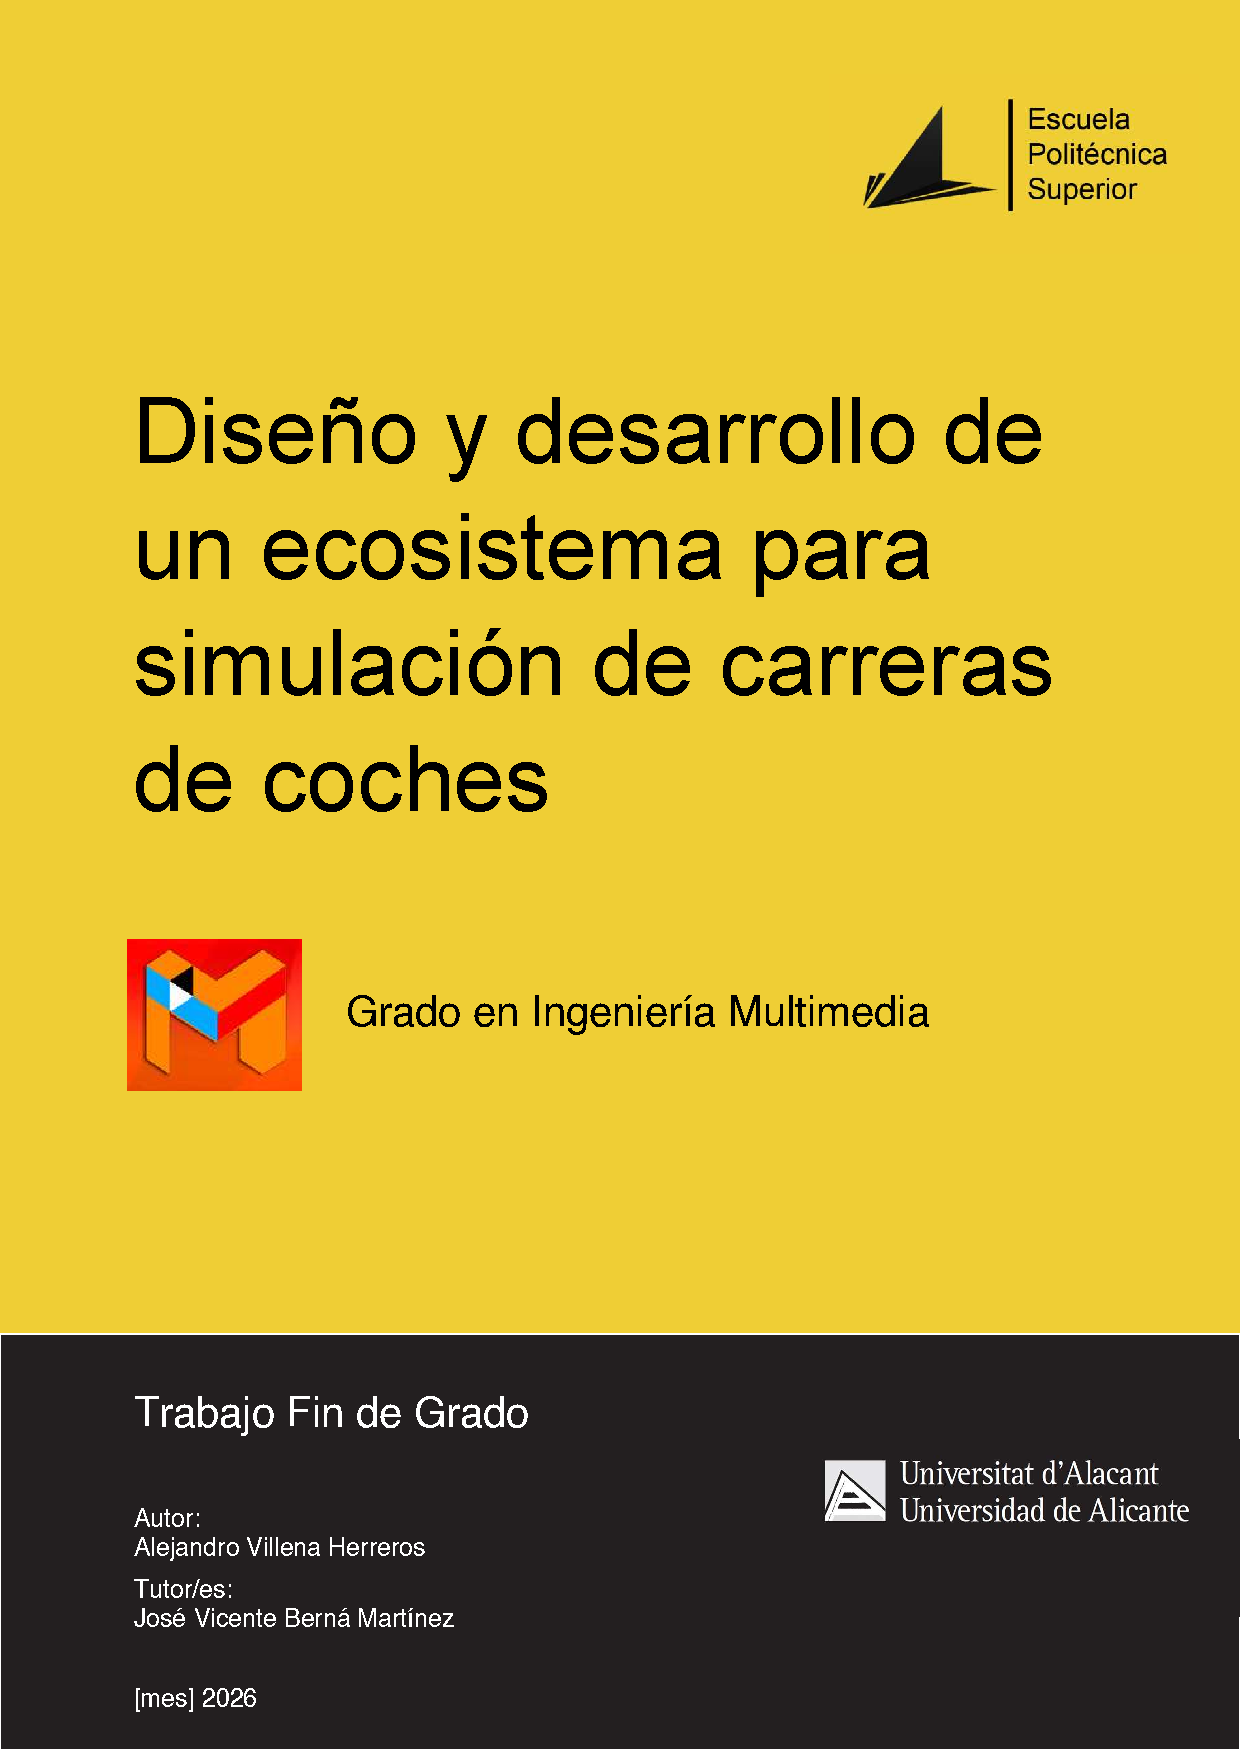
\includegraphics[width=\paperwidth]{img/portada.pdf}
			\vfill
		}%
	}%
}

% Página de la portada (con la imagen de fondo)
\thispagestyle{empty}
\mbox{}

% Hoja en blanco
\newpage
\thispagestyle{empty}
\mbox{}

% Portada interior
\begin{titlepage}
	\centering
	\vspace*{1.5cm}

	{\LARGE \textbf{Diseño y desarrollo de un ecosistema para simulación de carreras de coches}}\\[0.3cm]

	\vspace{0.3cm}
	\rule{\linewidth}{0.8pt}

	\vspace{2cm}

	\textbf{Autor:}\\[0.2cm]
	Alejandro Villena Herreros

	\vspace{1.5cm}

	\textbf{Tutor:}\\[0.2cm]
	José Vicente Berná Martínez \\
	Departamento de Tecnología Informática y Computación

	\vfill

	
\includegraphics[height=1.8cm]{img/logo_eps.png}
	\hspace{1.5cm}
	
\includegraphics[height=1.8cm]{img/logo_ua.jpg}

	\vspace{1cm}

	\textbf{ALICANTE, mes 2026}

\end{titlepage}

% Hoja en blanco tras la portada
\newpage
\thispagestyle{empty}
\mbox{}

	\pagenumbering{roman}
	\chapter*{Licencia}
La presente memoria se ha elaborado utilizando como base la plantilla \textit{Guía para
el Desarrollo de los Trabajos Fin de Grado y Fin de Máster}, confeccionada por José
Vicente Berná Martínez, bajo licencia Creative Commons Reconocimiento (CC BY).

\vspace{0.3cm}

\includegraphics[height=1cm]{img/licencia_by.png}

\vspace{0.5cm}

{\raggedright
Asimismo, esta obra se distribuye bajo licencia Creative Commons
Reconocimiento-\allowbreak NoComercial-\allowbreak SinObraDerivada 4.0 Internacional (CC BY-NC-ND 4.0).\par}

\bigskip
Se permite compartir y redistribuir el material en cualquier medio o formato, siempre
que se reconozca adecuadamente la autoría, no se utilice con fines comerciales y no se
modifique ni se generen obras derivadas.

\bigskip
Para consultar el texto completo de la licencia se ruega al lector acceda a: \newline
\url{https://creativecommons.org/licenses/by-nc-nd/4.0/}

\vspace{0.3cm}

\includegraphics[height=1cm]{img/licencia.png}

\newpage
\thispagestyle{empty}
\mbox{}

	% =====================================================================
%  RESUMEN EN CASTELLANO, VALENCIANO E INGLÉS
%  El título de cada página (Resumen / Resum / Abstract) lo pone babel
%  automáticamente según el idioma seleccionado.
% =====================================================================

\begin{abstract}
	Escribe aquí el resumen del trabajo en castellano.

	\bigskip
	\textbf{Palabras clave:} palabra 1, palabra 2, palabra 3.
\end{abstract}

\selectlanguage{catalan}
\begin{abstract}
	Escriu ací el resum del treball en valencià.

	\bigskip
	\textbf{Paraules clau:} paraula 1, paraula 2, paraula 3.
\end{abstract}

\selectlanguage{english}
\begin{abstract}
	Write the abstract of the project in English here.

	\bigskip
	\textbf{Keywords:} keyword 1, keyword 2, keyword 3.
\end{abstract}

\selectlanguage{spanish}   % volver al castellano para el resto

	\chapter*{Motivación y Justificación}
Escribe aquí la motivación personal y la justificación del trabajo.

	\chapter*{Agradecimientos}
Escribe aquí los agradecimientos.

	% Guía EPS 2.4: una única hoja, alineadas a la derecha y repartidas por la página
\chapter*{Citas}
\vspace*{\fill}
\begin{flushright}
	\emph{``Texto de la primera cita''}\\[0.5em]
	Autor
\end{flushright}
\vspace*{\fill}
\begin{flushright}
	\emph{``Texto de la segunda cita''}\\[0.5em]
	Autor
\end{flushright}
\vspace*{\fill}


	% ---------- ÍNDICES ----------
	% Guía EPS 2.5: contenidos, figuras, tablas y abreviaturas, en este orden y cada uno en página nueva
	\tableofcontents
	\listoffigures
	\listoftables
	\lstlistoflistings   % índice de código (bórralo si no usas listings)
	\printglossary[type=\acronymtype, title=Acrónimos]

	% ---------- CUERPO ----------
	\cleardoublepage
	\pagenumbering{arabic}
	\setcounter{page}{1}

	% !TeX root = ../main.tex
\chapter{Introducción}

Texto de la introducción. Ejemplos de uso de la plantilla:

\begin{itemize}[label=$\bullet$]
	\item Cita entre paréntesis: \citapendiente{}.
	\item Cita en el texto: según \citapendiente{}, \dots
	\item Término del glosario: una \gls{api} expone varios \glspl{endpoint}.
	\item Acrónimo (la primera vez sale completo): \gls{tfg}, y después \gls{tfg}.
	\item Nota a pie con enlace\footnote{\url{https://www.ejemplo.com}}.
	\item Nota pendiente en el margen.\todo{Revisar este párrafo}
\end{itemize}

% ---------- Figura ----------
\begin{figure}[H]
	\centering
	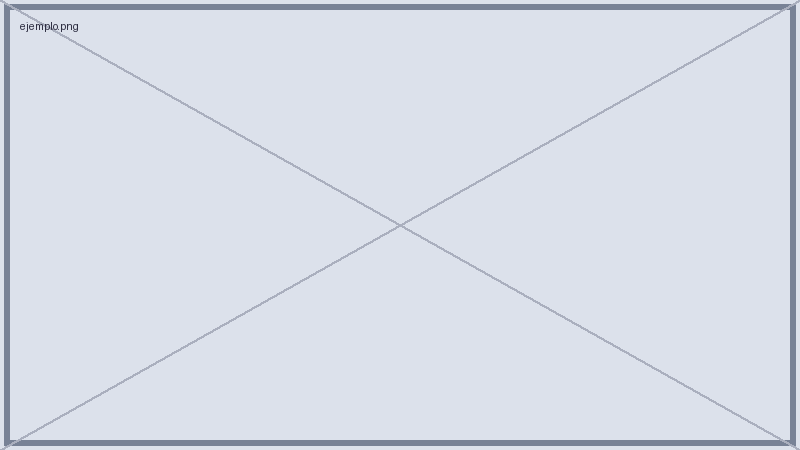
\includegraphics[width=0.6\linewidth]{img/ejemplo.png}
	\caption[Figura de ejemplo]{Figura de ejemplo. (Fuente propia)}
	\label{fig:ejemplo}
\end{figure}

Como se ve en la Figura~\ref{fig:ejemplo}, \dots

% ---------- Tabla ----------
\begin{table}[H]
	\centering
	\renewcommand{\arraystretch}{1.5}
	\begin{tabularx}{\textwidth}{p{3cm} >{\raggedright\arraybackslash}X}
		\textbf{Columna 1} & \textbf{Columna 2} \\
		\midrule
		Dato & Descripción más larga que se ajusta al ancho disponible. \\
		\midrule
		Dato & Otra descripción. \\
	\end{tabularx}
	\caption{Tabla de ejemplo}
	\label{tab:ejemplo}
\end{table}

% ---------- Código ----------
\begin{lstlisting}[language=JavaScript, style=codigo, caption={Código de ejemplo}, label={lst:ejemplo}]
// Comentario de ejemplo
export async function saludar(nombre) {
	const mensaje = "Hola, " + nombre;
	return mensaje;
}
\end{lstlisting}

	% !TeX root = ../main.tex
% NOTA: los cambios aparecen en azul. Requiere \usepackage{xcolor} en el preámbulo.
\chapter{Del problema a la solución: contexto y propuesta}
\label{cap:problema-solucion}
Este capítulo concreta el punto de partida, qué problema se quiere resolver y qué solución se propone para hacerlo, apoyándose en el análisis del sector y de los productos existentes que se desarrolla en el estado del arte (capítulo~\ref{cap:estado-arte}). En primer lugar se resume el contexto y se concreta el problema (sección~\ref{sec:contexto}). A continuación se presenta la propuesta, el ecosistema VH SimGrid, formado por tres periféricos y una aplicación de escritorio que los integra (sección~\ref{sec:propuesta}). Por último, se estudia la viabilidad de la propuesta desde los puntos de vista estratégico, de negocio, de riesgos y económico (sección~\ref{sec:viabilidad}).

\section{Contexto}
\label{sec:contexto}
El simracing ha pasado en poco más de una década de ser una afición minoritaria a convertirse en un mercado consolidado, con competiciones oficiales, equipos profesionales y cientos de miles de aficionados que compiten desde casa (sección~\ref{sec:simracing-entrenamiento}). Ese crecimiento se ha apoyado en la llegada al consumidor de tecnologías que antes eran exclusivas de la gama profesional, como las bases \textit{direct drive} o las pedaleras con célula de carga (sección~\ref{sec:fundamentos-tecnicos}). Sin embargo, el acceso a un equipo de simulación de calidad sigue encontrando tres obstáculos, que constituyen el problema que plantea este trabajo: los periféricos son caros, son cerrados y no existe un software que los una.

\paragraph{Periféricos caros.}
El periférico es el componente que más pesa en el coste de un equipo de simracing. Una base \textit{direct drive} de par medio se sitúa entre los 500 y los 850~euros: la Moza R12~V2, de 12~N\,m, tiene un precio oficial de 529~euros; la Fanatec ClubSport~DD, de 15~N\,m, de unos 600~euros, y la Simagic Alpha EVO Pro, de 18~N\,m, salió al mercado por 839~euros \parencite{moza_web, fanatec_web, bsimracing_2025_alpha_evo}. A la base hay que sumar el aro y la pedalera, que no son accesorios menores: un aro de tipo GT de gama media y una pedalera con célula de carga de dos pedales cuestan cada uno en torno a 400--450~euros en el catálogo del mismo fabricante \parencite{moza_web}. Un puesto completo de gama media supera así con facilidad los 1.200~euros, sin contar el \textit{cockpit} ni el ordenador. Como se detalla en el estado del arte, buena parte de ese precio no se explica por la tecnología, que se basa en componentes disponibles a bajo coste gracias a la robótica y a la movilidad eléctrica, sino por la marca, las licencias y los márgenes de un mercado dominado por pocos fabricantes (sección~\ref{sec:soluciones-comerciales}).

\paragraph{Periféricos cerrados.}
Cada fabricante construye su propio ecosistema y lo protege. El aro se une a la base mediante un anclaje rápido propietario, de modo que un aro de una marca no se puede montar en la base de otra sin un adaptador. El firmware y los protocolos de comunicación no son públicos: el usuario no puede saber cómo se calcula el \textit{force feedback} ni modificar su comportamiento más allá de los parámetros que el fabricante decide exponer. Esta dependencia tiene además un riesgo para el comprador, que queda ligado a la continuidad de la marca. El caso de Fanatec, cuya empresa matriz entró en concurso de acreedores en 2024 y acabó adquirida por Corsair \parencite{businesswire_2024_corsair_fanatec}, mostró que incluso el fabricante líder puede atravesar dificultades que ponen en duda el soporte de los productos ya vendidos (sección~\ref{sec:soluciones-comerciales}). Los proyectos abiertos DIY ofrecen una alternativa a este modelo, pero suelen centrarse en un único periférico y exigen al usuario conocimientos técnicos para montar y configurar el conjunto.

\paragraph{Sin un software que los una.}
El tercer obstáculo aparece una vez que el equipo está montado. Cada fabricante distribuye su propia aplicación de configuración, como Moza Pit House, Fanatec App o SimPro Manager, y un usuario que combina periféricos de varias marcas tiene que instalar y utilizar software de diferentes distribuidores. A ellas se suman las herramientas de apoyo al piloto como SimHub para las pantallas, los LEDs y la vibración, Crew Chief como ingeniero por voz y una o varias aplicaciones de análisis de telemetría (sección~\ref{sec:software-apoyo}). Cada programa tiene su instalación, sus perfiles y su forma de leer los datos del simulador, y ninguno conoce el hardware sobre el que se ejecuta: la herramienta que enciende los LEDs del aro no puede ajustar el \textit{force feedback} de la base ni la curva del freno. El resultado es un puesto fragmentado donde el usuario final tiene que configurar todo evitando problemas de compatibilidad, lo que puede llegar a ser frustrante y complicado para aquellos que no tienen experiencia.

\paragraph{Planteamiento del problema.}
De los tres obstáculos anteriores se deriva el problema que aborda este trabajo: no existe un sistema que ofrezca un puesto de simracing completo, con prestaciones de gama media y a un coste sensiblemente inferior al de los equipos comerciales, cuyos periféricos y cuyo software se hayan diseñado juntos. Resolverlo exige actuar a la vez sobre el hardware y sobre el software. En el hardware, creando periféricos propios a partir de componentes accesibles, sin depender del ecosistema de ningún fabricante. En el software, desarrollando una aplicación específica para esos periféricos, que los configure en vivo sin necesidad de reprogramarlos, de modo que resulte accesible para la mayor parte del público, que no tiene conocimientos de electrónica ni sabe grabar un firmware, y que reúna además las funciones que hoy se reparten entre programas independientes, como las pantallas de datos, el ingeniero por voz, la estrategia de carrera y el análisis de telemetría. Este es el planteamiento del sistema que se propone en la sección siguiente.


\section{Propuesta de valor}
\label{sec:propuesta}

Para resolver el problema planteado se propone desarrollar VH SimGrid, un ecosistema de simracing formado por tres periféricos de fabricación propia y una aplicación de escritorio diseñada específicamente para ellos. Los periféricos cubrirán los tres elementos básicos de un puesto de simulación: una base con \textit{force feedback}, la VH Grid DD15; una pedalera, la VH Axis, y un aro, el VH Formula Apex. La aplicación, que da nombre al conjunto, se encargará de configurarlos y reunirá además las funciones de apoyo al piloto que hoy se reparten entre programas independientes. La tabla~\ref{tab:ecosistema} resume el papel de cada componente.

\begin{table}[htbp]
	\centering
	\caption{Componentes del ecosistema VH SimGrid propuesto.}
	\label{tab:ecosistema}
	\small
	\begin{tabular}{|l|p{0.36\textwidth}|p{0.3\textwidth}|}
		\hline
		\textbf{Componente} & \textbf{Función} & \textbf{Enfoque} \\
		\hline
		VH Grid DD15 & Base con \textit{force feedback} que transmite al piloto las fuerzas de la dirección & Motor sin escobillas de bajo coste y controladora FOC con firmware propio \\
		\hline
		VH Axis & Pedalera de acelerador, freno y embrague & Sensores de posición y célula de carga en el freno \\
		\hline
		VH Formula Apex & Aro de tipo Fórmula con mandos e indicadores luminosos & Microcontrolador, matriz de botones y LEDs \\
		\hline
		VH SimGrid & Configuración de los periféricos y apoyo al piloto en un único programa & Aplicación de escritorio para Windows \\
		\hline
	\end{tabular}
\end{table}

El planteamiento responde directamente a los tres obstáculos identificados en la sección~\ref{sec:contexto}. Frente al coste, los periféricos se construirán con componentes de bajo precio procedentes de la robótica, la movilidad eléctrica y la electrónica de aficionado, que funcionan según los mismos principios que los periféricos comerciales. Frente a los ecosistemas cerrados, todos los periféricos se presentarán al ordenador como dispositivos USB estándar, de modo que cualquier simulador pueda usarlos sin controladores específicos. Frente a la fragmentación del software, los periféricos y la aplicación se diseñarán juntos, para que la aplicación conozca cada dispositivo y pueda ajustarlo, y reúna en un solo programa la configuración y las herramientas de apoyo al piloto.

A estos tres criterios se suma un cuarto: que el sistema pueda usarlo alguien sin conocimientos técnicos. Una vez montados los periféricos, el usuario no debería tener que programar ni grabar firmware para configurarlos. Los ajustes se harán desde la aplicación y se aplicarán en vivo, y las actualizaciones de firmware se instalarán también desde ella, con la menor intervención posible. Las subsecciones siguientes describen la propuesta para cada componente.

\subsection{Base de \textit{force feedback}}
\label{sec:propuesta-base}

La base, que recibirá el nombre de VH Grid DD15, es el periférico que más influye en la experiencia de conducción y también el más caro, por lo que es el componente central de la propuesta. Su objetivo es ofrecer un \textit{force feedback} comparable al de las bases \textit{direct drive} de gama media del mercado con un coste muy inferior.

\paragraph{Enfoque.}
Se adoptará la arquitectura \textit{direct drive}, en la que el aro se monta directamente sobre el eje del motor, porque es la única que transmite la señal del simulador sin las holguras, la elasticidad y el rozamiento de una transmisión por engranajes o por correa (véase la sección~\ref{sec:bases-ffb}). La dificultad de esta arquitectura no está en la mecánica, sino en el motor y en su control. Para el motor se plantea reutilizar un motor de buje sin escobillas de los que se fabrican en grandes series para vehículos de movilidad personal como patinetes eléctricos, que por su construcción dan mucho par a baja velocidad y cuestan una fracción de un servomotor específico. Para el control se partirá de una controladora de código abierto con control vectorial (FOC), sobre la que se desarrollará un firmware propio que la convierta en una base de \textit{force feedback}.

\paragraph{Funciones previstas.}
La base deberá presentarse ante el sistema operativo como un volante de \textit{force feedback} estándar mediante la clase HID PID, la extensión del estándar USB para dispositivos que generan fuerzas, de modo que los simuladores la reconozcan sin controladores y le envíen sus efectos a través de la interfaz DirectInput de Windows (véase la sección~\ref{sec:fundamentos-tecnicos}). Entre la consigna del simulador y el par del motor, el firmware aplicará una cadena de procesado ajustable desde la aplicación de los que cuenta el rango de giro, la fuerza máxima, una curva de respuesta, un filtrado por frecuencias que permita realzar o atenuar distintos tipos de efecto y perfiles que se carguen según el simulador o el tipo de coche. Además, deberá compensar el \textit{cogging} propio de los motores de buje, que de otro modo se notaría como pequeños saltos al girar el volante.

\paragraph{Seguridad.}
Una base \textit{direct drive} puede generar un par capaz de lesionar las manos o las muñecas del piloto, especialmente en un choque o si el volante se suelta a alta velocidad. Por ello, la seguridad se considera un requisito de diseño y no un añadido: el firmware deberá limitar el par y la velocidad, proteger el motor frente al sobrecalentamiento y frenar el volante en los límites establecidos, con independencia de lo que pida el simulador.



\subsection{Pedalera}
\label{sec:propuesta-pedalera}

La pedalera, que recibirá el nombre de VH Axis, recogerá las órdenes del piloto sobre el acelerador, el freno y el embrague. Después de la base, es el periférico que más influye en la consistencia del piloto, porque de ella depende que pueda repetir una frenada vuelta tras vuelta. Su objetivo es ofrecer las prestaciones de una pedalera de gama media, con freno por célula de carga y los otros dos mediante recorrido usando sensores Hall, a un coste muy inferior al de los modelos comerciales equivalentes.

\paragraph{Enfoque.}
La decisión de diseño más importante es qué magnitud mide cada pedal. En un coche real, el pedal de freno apenas se desplaza y el piloto dosifica la frenada con la presión del pie, mientras que el acelerador y el embrague se controlan por su posición (véase la sección~\ref{sec:pedaleras}). Por ello se plantea una solución mixta. El freno medirá la fuerza mediante una célula de carga, un sensor que produce una señal proporcional a la fuerza aplicada. El acelerador y el embrague medirán su recorrido con sensores de efecto Hall, que detectan la posición de un imán sin contacto físico y, por tanto, no se desgastan ni generan el ruido de los potenciómetros que montan las pedaleras de gama de entrada. La estructura y los pedales serán de fabricación propia, con elementos elásticos que den al freno una resistencia progresiva, y un microcontrolador leerá los tres sensores y se comunicará con el ordenador.

\paragraph{Funciones previstas.}
La pedalera se presentará ante el sistema operativo como un mando USB estándar con tres ejes, por lo que cualquier simulador podrá usarla sin controladores. El microcontrolador leerá los sensores a una frecuencia elevada y filtrará su ruido, de modo que la señal llegue al simulador estable y sin retraso apreciable. Desde la aplicación, el usuario podrá calibrar cada pedal de forma guiada, indicando su posición de reposo y su máximo recorrido, y en el caso del freno, la fuerza máxima en kilogramos que desea aplicar. También podrá ajustar la curva de respuesta de cada pedal, que modifica la relación entre el pie del piloto y el valor que recibe el simulador, así como las zonas muertas al principio y al final del recorrido. Estos ajustes se guardarán en la memoria de la propia pedalera, de modo que se conserven aunque se conecte a otro ordenador o la aplicación no esté abierta.

\subsection{Aro}
\label{sec:propuesta-aro}

El aro, que recibirá el nombre de VH Formula Apex, es la parte del volante que el piloto sujeta y desde la que maneja los mandos del coche sin soltar las manos. En los periféricos comerciales es también el componente en el que el precio depende menos de la tecnología siendo su electrónica sencilla, y las réplicas de volantes reales alcanzan precios superiores al de una base completa por sus licencias y sus materiales (véase la sección~\ref{sec:soluciones-comerciales}). Su objetivo es ofrecer un aro de tipo Fórmula, con los mandos y los indicadores de un volante de competición actual, fabricado con medios propios.

\paragraph{Enfoque.}
Se plantea un aro de tipo Fórmula, de pequeño diámetro y con los mandos concentrados en su parte central, que toma como referencia el volante del Aston Martin AMR23, el monoplaza con el que Fernando Alonso disputó la temporada 2023 del Campeonato del Mundo de Fórmula~1. El cuerpo del aro será de fabricación propia mediante impresión 3D, un proceso que permite iterar el diseño con rapidez y ajustar la forma de las empuñaduras y la posición de cada mando. Un microcontrolador leerá todos los mandos y gobernará los indicadores luminosos. Para leer un número elevado de pulsadores con pocos pines se empleará una matriz de botones, y los selectores rotativos se resolverán con \textit{encoders}. El aro se unirá a la base mediante un anclaje mecánico y tendrá su propia conexión con el ordenador, de modo que no dependa de un conector propietario y pueda montarse sobre otras bases.

\paragraph{Funciones previstas.}
El aro incluirá pulsadores, \textit{encoders}, levas de cambio y levas de embrague, que el ordenador reconocerá como los botones y ejes de un mando USB estándar, por lo que cualquier simulador podrá asignarlos sin controladores. Las levas de embrague podrán funcionar como un embrague convencional o con un punto de mordida ajustable, para facilitar las salidas. En la parte superior, una tira de LEDs mostrará las revoluciones del motor y avisará de los eventos de la carrera, como las banderas, la actuación de ayudas electrónicas del vehículo, el limitador de velocidad en el \textit{pit lane} o la presencia de otros coches cerca. En el centro del aro, como en los volantes de Fórmula~1, una pantalla mostrará al piloto la información de la carrera como la marcha engranada, las revoluciones, el tiempo por vuelta y la diferencia con la vuelta de referencia, el combustible o el estado de los neumáticos. Su contenido lo generará la aplicación a partir de la telemetría del simulador, podrá organizarse en varias páginas que el piloto pase con los botones del aro y se diseñará con el mismo editor que las pantallas de datos de la aplicación (véase la sección~\ref{sec:propuesta-app}). Todo ello se configurará desde la aplicación, pudiendo elegir qué efecto se muestra en cada LED, con qué colores y con qué estilo, el umbral de revoluciones de cada luz y el brillo, con perfiles que se carguen según el simulador y el coche. Como en el resto de periféricos, los ajustes básicos se guardarán en el propio aro para que funcione aunque la aplicación no esté abierta.

\subsection{Aplicación de escritorio}
\label{sec:propuesta-app}

La aplicación de escritorio, que da nombre al ecosistema, VH SimGrid, es la pieza que une los periféricos y la que responde al tercer obstáculo identificado en la sección~\ref{sec:contexto}: la falta de un software que los integre. Su objetivo es que el piloto pueda configurar todo su puesto y disponer de las herramientas de apoyo que necesita desde un único programa, sin conocimientos técnicos y sin tener que instalar y coordinar aplicaciones de distintos fabricantes.

\paragraph{Enfoque.}
Se plantea una aplicación de escritorio para Windows, el sistema operativo en el que se ejecutan la mayoría de los simuladores de PC, organizada en páginas y utilizadas una para cada periférico y una para cada herramienta de apoyo. La aplicación tendrá dos fuentes de información. Por un lado, se comunicará con los periféricos para leer su estado y enviarles los ajustes. Por otro, leerá la telemetría que publica cada simulador, es decir, los datos del coche y de la carrera en cada instante. Como cada simulador publica esos datos en su propio formato (véase la sección~\ref{sec:software-apoyo}), la aplicación incluirá una capa que los traduzca a un formato común, de modo que el resto de funciones trabajen igual con cualquier simulador compatible. Toda la información se procesará en el propio equipo del usuario, sin enviar datos a servicios externos.

\paragraph{Configuración de los periféricos.}
La aplicación detectará los periféricos al conectarlos y mostrará su estado en una pantalla de inicio, junto con los simuladores instalados. La primera vez, un asistente guiará al usuario en la configuración de cada periférico y de la telemetría de sus juegos. Desde ella se ajustarán el \textit{force feedback} de la base, la calibración y las curvas de los pedales y las luces del aro, como se ha descrito en las subsecciones anteriores. Los cambios se aplicarán en vivo y se agruparán en perfiles que podrán cargarse automáticamente al detectar el simulador o el coche en uso. La aplicación se encargará también de actualizar el firmware de los periféricos cuando haya una versión nueva, de modo que el usuario no tenga que usar herramientas de programación.

\paragraph{Pantallas de datos.}
La aplicación incluirá un \textit{dash}, una pantalla de datos como la de un coche de competición, que mostrará en la pantalla central del aro o en un monitor secundario información como la marcha, las revoluciones, los tiempos por vuelta, el estado de los neumáticos o el combustible. Se ofrecerá una colección de diseños de serie para distintos tipos de coche y un editor con el que el usuario pueda crear los suyos o modificar los existentes a partir de elementos como textos, indicadores, barras o gráficas.

\paragraph{Ingeniero de pista por voz.}
La aplicación incorporará un ingeniero de pista virtual que informará al piloto por voz durante la carrera, como haría el ingeniero de un equipo real por la radio: avisos de coches cerca, consumo de combustible, estado de los neumáticos, ritmo, diferencias con los rivales o momento de entrar a boxes. El piloto podrá también preguntarle por voz, pulsando un botón del aro asignado, sin soltar el volante. Para preparar las carreras largas, la aplicación incluirá además una calculadora de estrategia que compare distintas opciones de paradas según el reglamento de cada carrera, y la estrategia elegida será la que siga el ingeniero durante la prueba. Tanto la síntesis de voz como el reconocimiento de lo que dice el piloto funcionarán en el propio equipo.

\paragraph{Análisis de telemetría.}
Por último, la aplicación grabará automáticamente cada sesión y permitirá analizarla después, al estilo de las herramientas de análisis de datos del automovilismo profesional. El piloto podrá comparar sus vueltas con una de referencia y estudiar, canal a canal y curva a curva, la velocidad, el uso de los pedales, el giro del volante, el comportamiento de los neumáticos o la suspensión, para encontrar dónde pierde tiempo y cómo mejorar su conducción.

\section{Estudio de viabilidad}
\label{sec:viabilidad}

Antes de comenzar el desarrollo conviene comprobar que la propuesta es viable, es decir, que tiene sentido frente a las alternativas existentes, que puede llevarse a cabo con los medios disponibles y que los riesgos que implica son asumibles. Aunque este trabajo es un proyecto académico, la propuesta se analiza como si fuera un producto, porque solo así puede valorarse si resuelve de verdad el problema planteado para un usuario real. El estudio se aborda desde cuatro puntos de vista complementarios: la posición estratégica de la propuesta frente al mercado, mediante un análisis DAFO (sección~\ref{sec:dafo}); su modelo de negocio, mediante un Lean Canvas (sección~\ref{sec:lean-canvas}); los riesgos del proyecto y su plan de mitigación (sección~\ref{sec:riesgos}), y su viabilidad económica, {\color{blue}mediante el análisis de los recursos disponibles y un presupuesto estimado} (sección~\ref{sec:viabilidad-economica}).

\subsection{Análisis DAFO}
\label{sec:dafo}

El análisis DAFO es una herramienta de planificación estratégica que examina una propuesta desde dos dimensiones. En la dimensión interna se recogen las debilidades y las fortalezas, que dependen del propio proyecto y de las decisiones que se tomen en él. En la dimensión externa se recogen las amenazas y las oportunidades, que proceden del mercado y del entorno y que el proyecto no puede controlar, pero sí aprovechar o prevenir \parencite{weihrich_1982_tows}. La figura~\ref{fig:dafo} resume el análisis de VH SimGrid, que se comenta a continuación.

\begin{figure}[H]
	\centering
	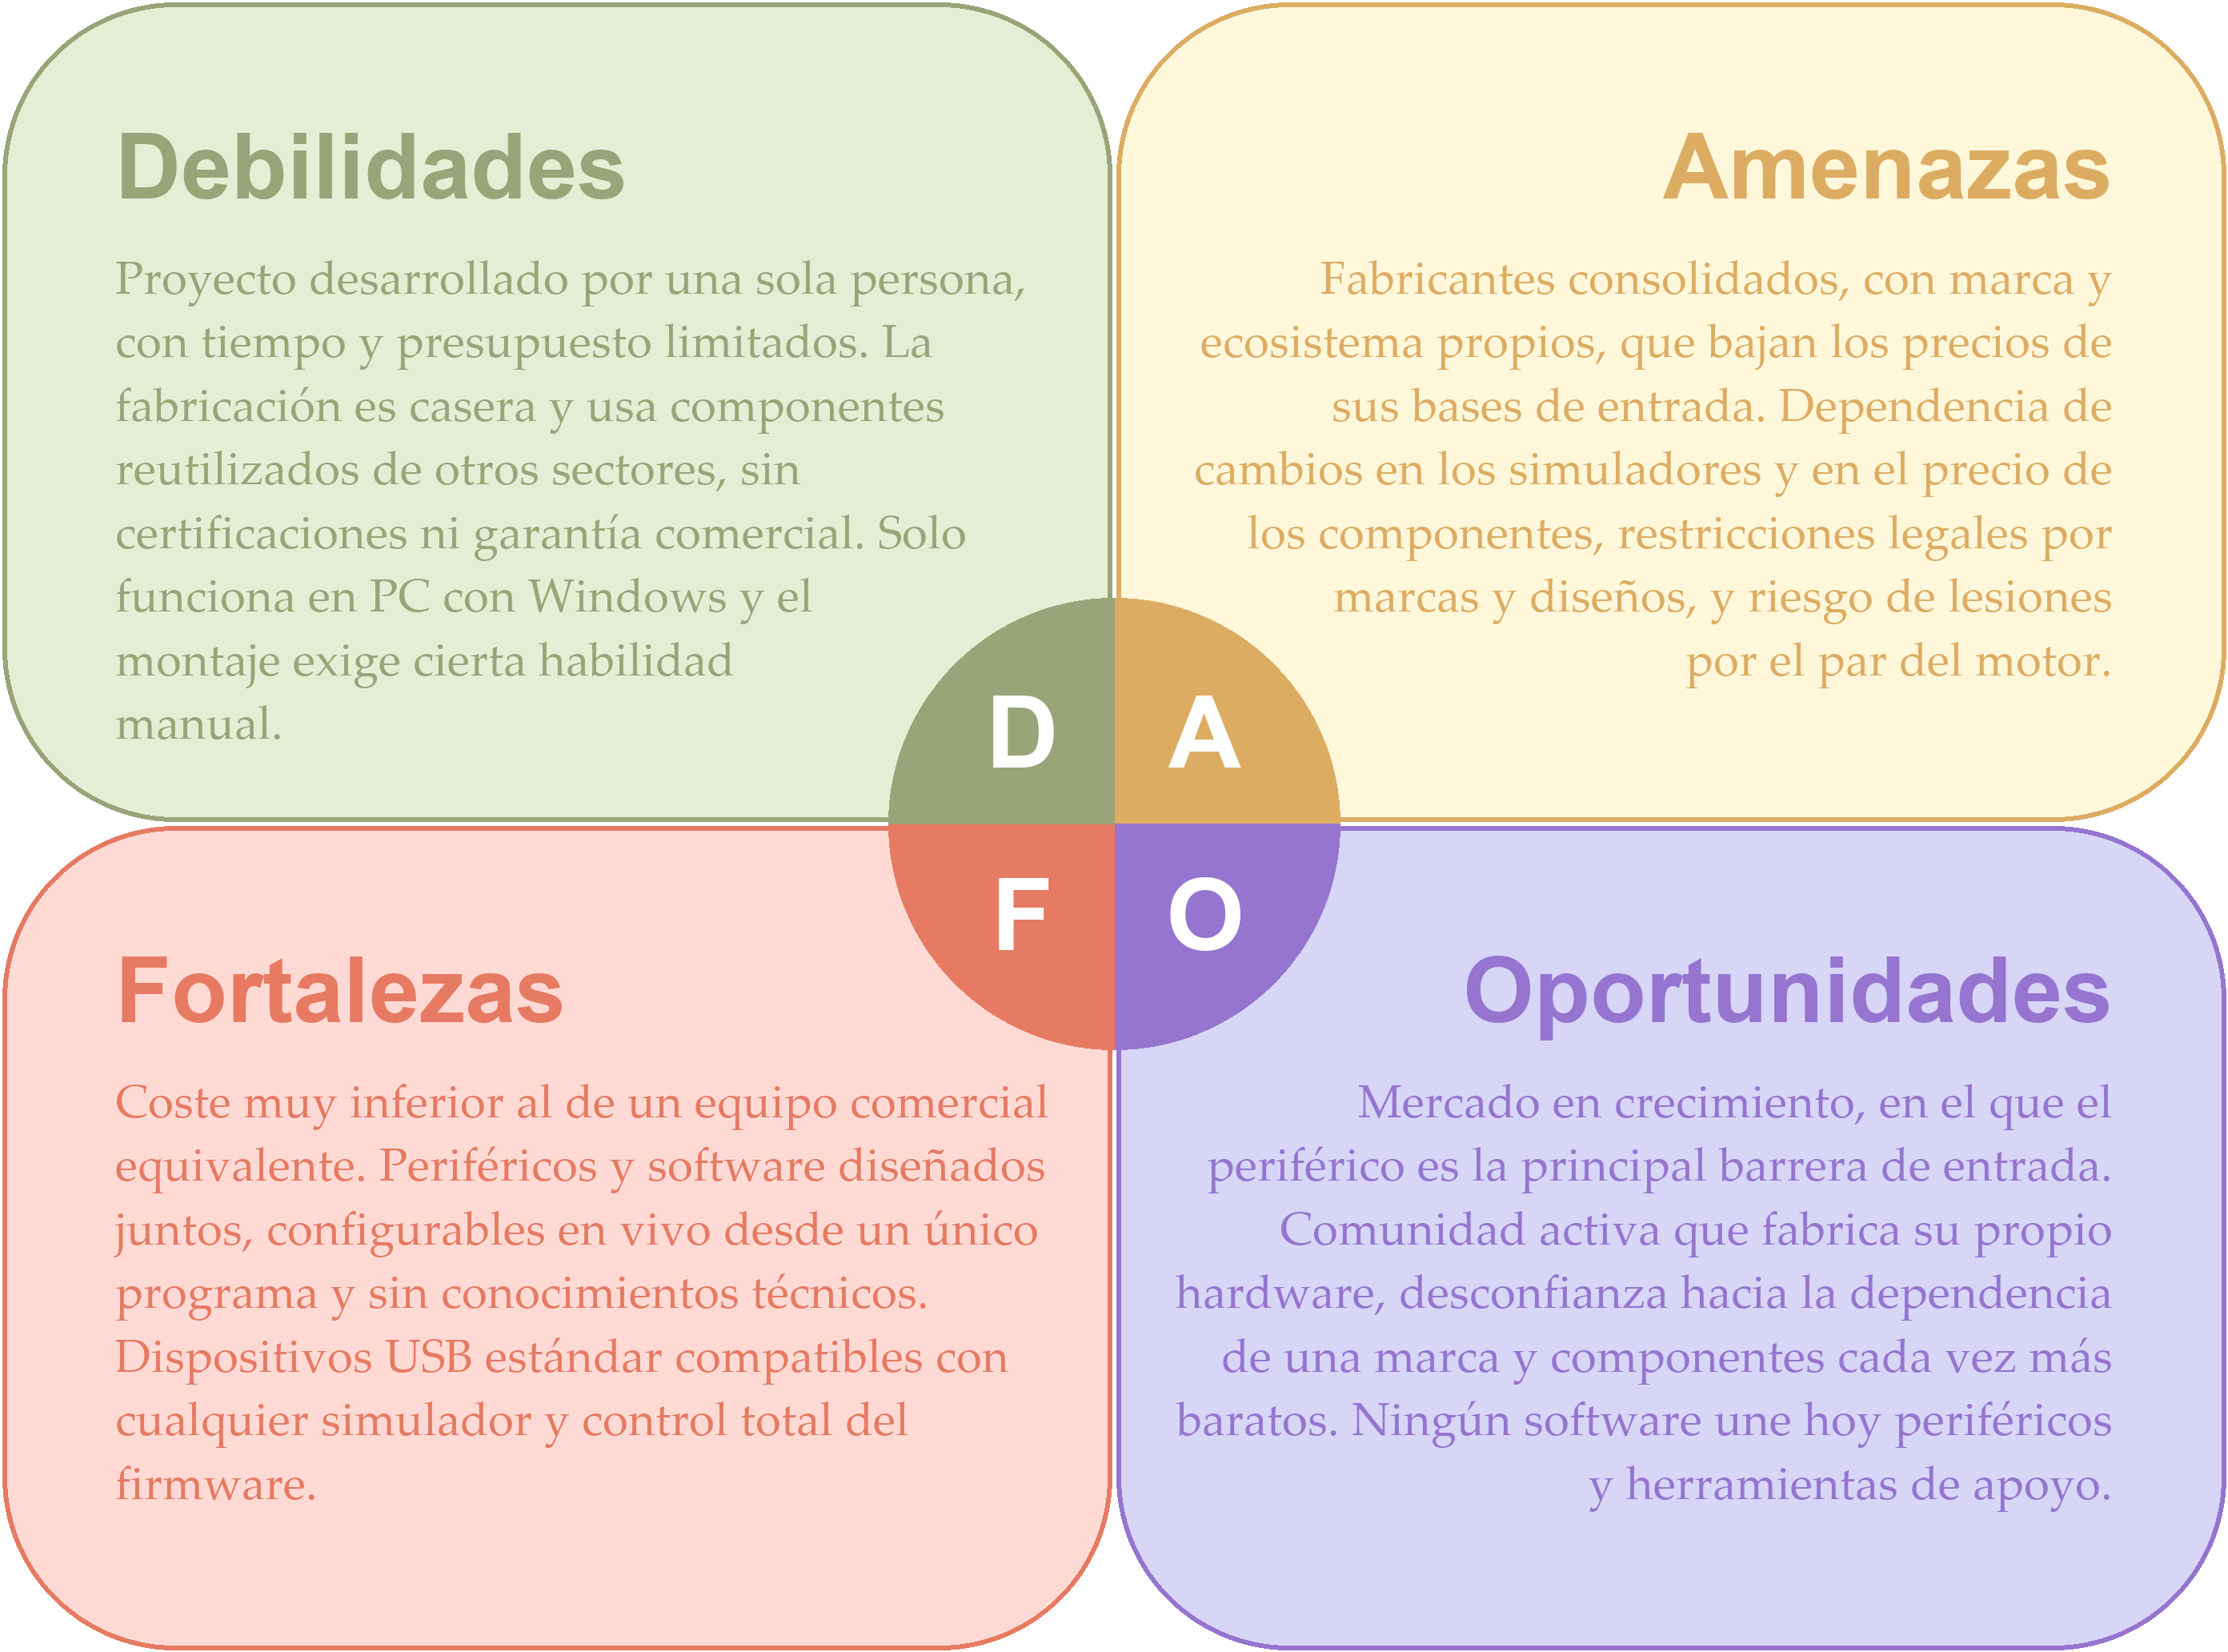
\includegraphics[width=\textwidth]{img/DAFO.png}
	\caption[Análisis DAFO del ecosistema VH SimGrid]{Análisis DAFO del ecosistema VH SimGrid. (Fuente propia)}
	\label{fig:dafo}
\end{figure}

\paragraph{Debilidades.}
La principal debilidad del proyecto es su escala. Lo desarrolla una sola persona, con un tiempo y un presupuesto limitados, frente a fabricantes con equipos de ingeniería completos. La fabricación casera, basada en la impresión 3D y en piezas mecanizadas a mano, no alcanza el acabado ni, previsiblemente, la durabilidad de un producto industrial, y los componentes clave, como el motor de la base, se reutilizan de otros sectores y no se han diseñado para esta aplicación. El sistema tampoco contará con certificaciones ni con la garantía de un producto comercial. Por último, la propuesta se limita al PC con Windows, mientras que una parte del mercado juega en consolas, y montar los periféricos exige cierta habilidad manual, aunque su configuración posterior no requiera conocimientos técnicos.

\paragraph{Amenazas.}
El mercado de periféricos evoluciona rápido. Los fabricantes han ido bajando el precio de sus bases \textit{direct drive} de entrada, que en algunos casos ya se sitúa en torno a los 330~euros \parencite{fanatec_web}, y cuentan con una marca reconocida, una comunidad de usuarios y ecosistemas completos de productos compatibles. El proyecto depende además de factores externos: los simuladores pueden cambiar el formato de su telemetría, el sistema operativo puede modificar la forma en que gestiona los dispositivos de \textit{force feedback}, y el precio y la disponibilidad de los componentes electrónicos pueden variar, como ocurrió durante la escasez de chips de 2021 \parencite{endor_web}. Tomar como referencia el volante de un monoplaza real plantea restricciones de propiedad intelectual sobre marcas y diseños. Y, sobre todo, una base \textit{direct drive} genera un par capaz de causar lesiones, una responsabilidad que en un producto comercial asume el fabricante.

\paragraph{Fortalezas.}
Frente a esas limitaciones, la propuesta tiene ventajas claras. La primera es el coste ya que al construirse con componentes de bajo precio, un equipo completo debería costar una fracción de su equivalente comercial. La segunda, y la más diferencial, es que los periféricos y el software se diseñan juntos. Esto permite que un único programa configure todo el puesto y reúna las herramientas de apoyo al piloto que en el mercado obligan a combinar varias aplicaciones, algo que ningún fabricante ni proyecto de fabricación propia ofrece hoy. A ello se suman la configuración en vivo, pensada para usuarios sin conocimientos técnicos; el uso de estándares USB, que hace los periféricos compatibles con cualquier simulador sin controladores; el control completo del firmware, que permite ajustar el comportamiento de cada periférico y ampliarlo, y el procesamiento local de los datos, que protege la privacidad del usuario.

\paragraph{Oportunidades.}
El contexto también es favorable. El simracing es un mercado en crecimiento en el que el periférico es la principal barrera de entrada, de modo que una alternativa de bajo coste responde a una necesidad real. Existe una comunidad activa de aficionados que diseñan y construyen su propio hardware, y que demanda precisamente herramientas que faciliten ese proceso. Las dificultades que han atravesado algunos fabricantes han hecho visible el riesgo de depender de una sola marca. La impresión 3D doméstica y los componentes procedentes de la movilidad eléctrica y la robótica son cada vez más baratos y accesibles. Y no existe un software que unifique la configuración de los periféricos con las herramientas de apoyo al piloto, un hueco que la propuesta ocupa directamente. Por último, una arquitectura común para periféricos y aplicación facilita ampliar el ecosistema en el futuro con nuevos dispositivos.

\paragraph{Conclusiones del análisis.}
El análisis muestra que la propuesta tiene sentido estratégico si se apoya en lo que la diferencia, este sistema, no compite con los fabricantes en acabado ni en marca, sino en coste y en integración entre hardware y software. Las fortalezas permiten aprovechar las principales oportunidades, como la demanda de alternativas baratas y la ausencia de un software unificado. Las debilidades y las amenazas, en cambio, se concentran en tres ámbitos que condicionan el diseño: la seguridad de la base, la dependencia de componentes y simuladores de terceros y las cuestiones legales. Estos riesgos se analizan en detalle en la sección~\ref{sec:riesgos}, junto con las medidas previstas para mitigarlos.

\subsection{Lean Canvas}
\label{sec:lean-canvas}

El Lean Canvas es una adaptación del \textit{Business Model Canvas} propuesta por Ash Maurya para proyectos en fase inicial, en los que todavía no existe un producto ni clientes y la mayor parte del modelo de negocio son hipótesis que hay que validar \parencite{maurya_2012_running_lean}. Resume el modelo en una sola página con nueve bloques: el problema, los segmentos de clientes, la propuesta de valor única, la solución, los canales, las fuentes de ingresos, la estructura de costes, las métricas clave y la ventaja diferencial. Frente al modelo original, pone el foco en el problema y en el cliente antes que en los socios o los recursos, lo que lo hace adecuado para un proyecto como este, que parte de una necesidad identificada y no de una empresa ya constituida. La figura~\ref{fig:lean-canvas} recoge el Lean Canvas de VH SimGrid, cuyos bloques se comentan a continuación agrupados por afinidad.

\afterpage{%
	\begin{landscape}
		\thispagestyle{empty}
		\begin{figure}[H]
			\centering
			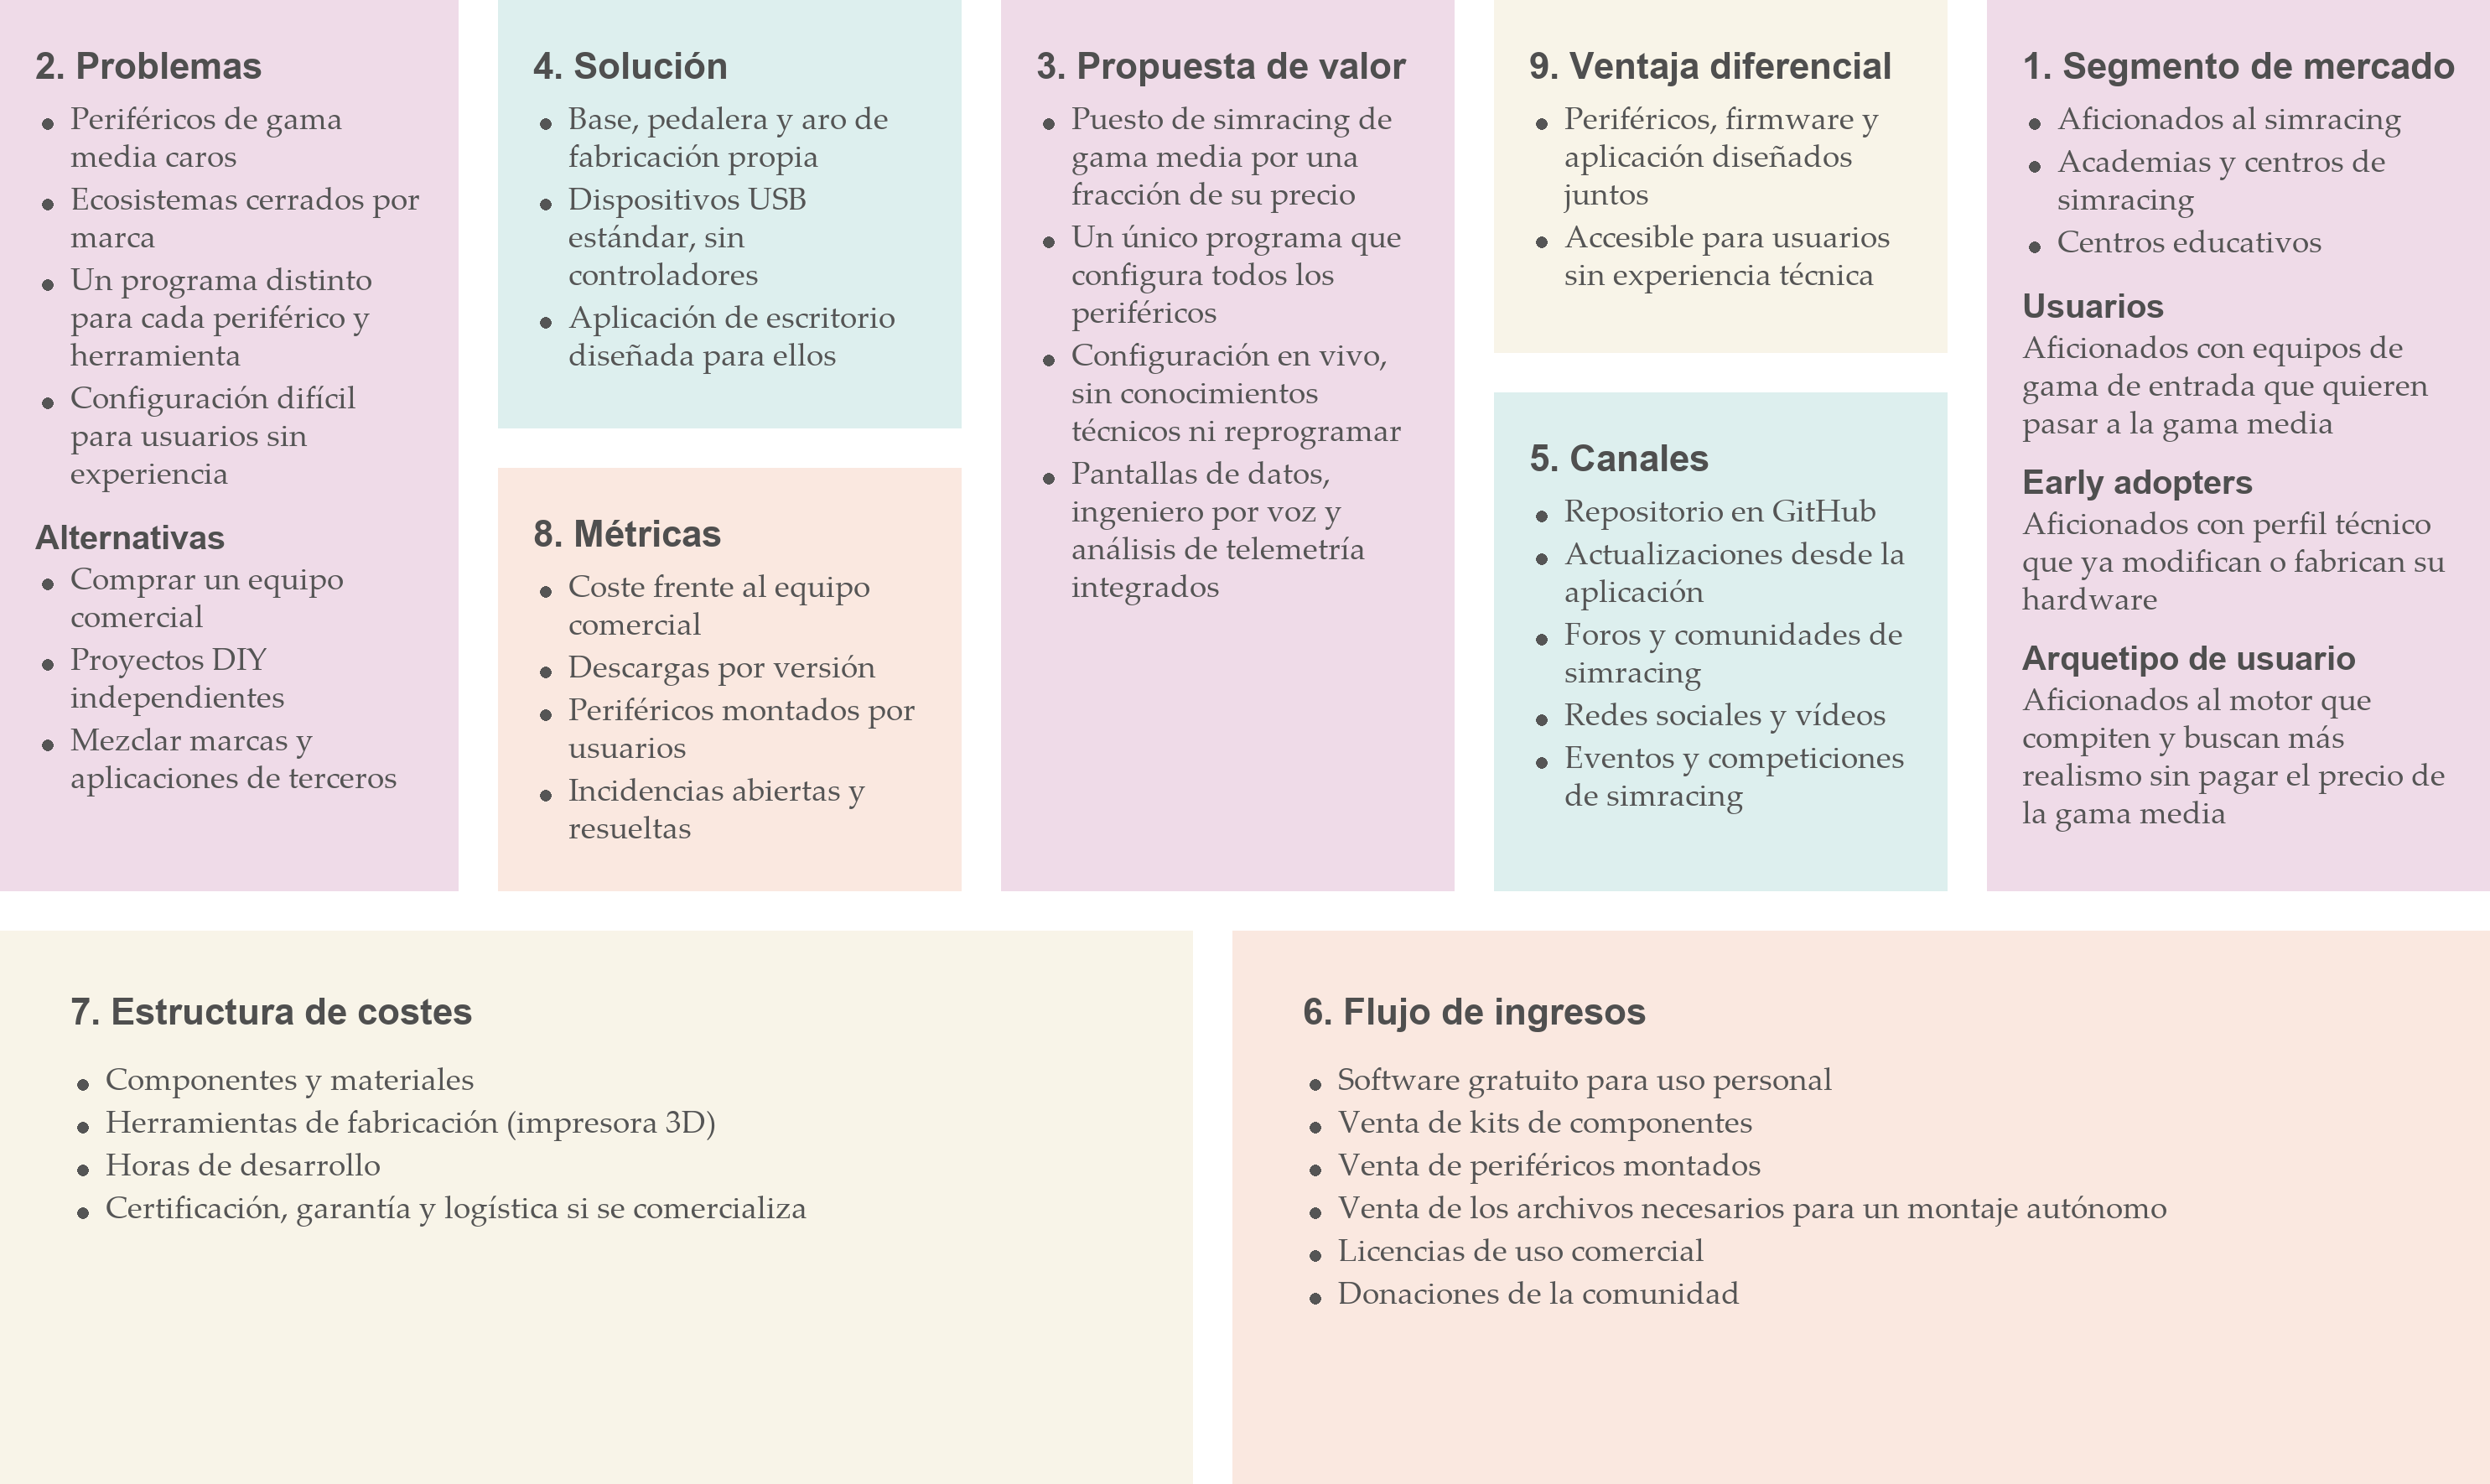
\includegraphics[width=0.9\linewidth, height=0.88\textheight, keepaspectratio]{img/Lean-Canvas.png}
			\caption[Lean Canvas del ecosistema VH SimGrid]{Lean Canvas del ecosistema VH SimGrid. (Fuente propia)}
			\label{fig:lean-canvas}
		\end{figure}
	\end{landscape}
}

\paragraph{Problema y segmentos de clientes.}
El segmento de mercado al que se dirige la propuesta está formado por tres grupos: los aficionados al simracing, las academias y centros de simracing y los centros educativos. Dentro de él, los usuarios principales son los aficionados que ya disponen de un equipo de gama de entrada y quieren dar el salto a la gama media, mientras que los primeros usuarios (\textit{early adopters}) serán los aficionados con perfil técnico que ya modifican o fabrican su propio hardware, dispuestos a montar un periférico si el resultado compensa el esfuerzo. El arquetipo de usuario es el de un aficionado al motor que compite en simuladores y busca más realismo sin pagar el precio de la gama media. 
Los problemas que comparten estos usuarios son los descritos en la sección~\ref{sec:contexto}: los periféricos de gama media son caros, cada fabricante encierra al usuario en su propio ecosistema, cada periférico y cada herramienta de apoyo requiere su propio programa, y configurar el conjunto resulta difícil para quien no tiene experiencia. Hoy existen tres alternativas para resolverlos, que son aquellas con las que compite la propuesta: comprar un equipo comercial y asumir su precio, construir los periféricos a partir de proyectos de fabricación propia independientes entre sí, o combinar periféricos de distintas marcas con varias aplicaciones de terceros.

\paragraph{Propuesta de valor y solución.}
La propuesta de valor de VH SimGrid es ofrecer un puesto de simracing de gama media por una fracción de su precio, configurado desde un único programa que gestiona todos los periféricos. Esa configuración se hará en vivo, sin conocimientos técnicos y sin necesidad de reprogramar los dispositivos, y el mismo programa integrará las pantallas de datos, el ingeniero de pista por voz y el análisis de telemetría que hoy obligan a combinar varias aplicaciones. La solución que materializa esta propuesta es el ecosistema descrito en la sección~\ref{sec:propuesta}: una base, una pedalera y un aro de fabricación propia que funcionan como dispositivos USB estándar, sin controladores, y una aplicación de escritorio diseñada específicamente para ellos.

\paragraph{Canales, fuentes de ingresos y estructura de costes.}
El canal principal de distribución será un repositorio público en GitHub, desde el que se publicarán el instalador de la aplicación y los firmwares de cada versión, y la propia aplicación avisará de las actualizaciones al usuario. Para dar a conocer el proyecto se emplearán los canales en los que se concentra la comunidad: foros y comunidades de simracing, redes sociales y plataformas de vídeo, en las que mostrar los periféricos en funcionamiento es la forma más eficaz de llegar al público, y eventos y competiciones de simracing. 
En cuanto al flujo de ingresos, el software se distribuirá de forma gratuita para uso personal, lo que permite construir una base de usuarios sobre la que apoyar el resto de fuentes: la venta de kits de componentes, la venta de periféricos ya montados para quien no quiera fabricarlos, la venta de los archivos necesarios para que el usuario realice un montaje autónomo, como los modelos para impresión 3D, las licencias de uso comercial para academias y centros de simracing y las donaciones de la comunidad. 
La estructura de costes, al no existir una empresa ni una plantilla, se reduce a los componentes y materiales, las herramientas de fabricación, principalmente la impresora 3D, y las horas de desarrollo, que son con diferencia el coste principal y se {\color{blue}estiman} en la sección~\ref{sec:viabilidad-economica}. Una eventual comercialización añadiría los costes de certificación, garantía y logística.

\paragraph{Métricas clave y ventaja diferencial.}
Las métricas que permitirán comprobar si la propuesta funciona son cuatro. La primera es el coste de un puesto completo frente al de un equipo comercial equivalente, que mide directamente el cumplimiento de la propuesta de valor. Las otras tres miden la adopción y la calidad del sistema una vez publicado: el número de descargas de cada versión, el número de periféricos montados por otros usuarios y las incidencias abiertas y resueltas en el repositorio. Como la aplicación procesa todos los datos en local y no envía información fuera del equipo, estas métricas se obtendrán de los canales públicos y no del uso de la aplicación. Por último, la ventaja diferencial del proyecto es que los periféricos, su firmware y la aplicación se diseñan juntos, una integración que no ofrecen los fabricantes comerciales, sin incentivos para abrir sus ecosistemas a periféricos ajenos, ni los proyectos de fabricación propia, centrados en un único periférico. A ello se suma que el sistema es accesible para usuarios sin experiencia técnica, lo que amplía su público más allá de los aficionados a la electrónica.

\subsection{Análisis de riesgos}
\label{sec:riesgos}

Todo proyecto está expuesto a sucesos que, si se producen, pueden retrasarlo, encarecerlo o impedir que alcance sus objetivos. El análisis de riesgos consiste en identificar esos sucesos antes de que ocurran, estimar su probabilidad y su impacto, y prever las medidas que los evitan o reducen sus consecuencias. En este proyecto los riesgos se agrupan en tres categorías: técnicos, de planificación y coste, y legales. Para cada uno se estima la probabilidad de que ocurra y el impacto que tendría sobre el proyecto en una escala de tres niveles (baja, media y alta), y la combinación de ambas determina su nivel de riesgo y la prioridad con la que debe atenderse{\color{blue}, según los criterios que se definen a continuación}.

{\color{blue}
	\paragraph{Escalas de valoración.}
	Para que la valoración de cada riesgo no dependa de una impresión subjetiva, cada nivel de la escala se asocia a un criterio concreto, recogido en la tabla~\ref{tab:escalas-riesgo}. La probabilidad se expresa por la frecuencia con la que se espera que el suceso se presente durante el desarrollo, que se prevé de unos seis meses. El impacto se mide por sus consecuencias sobre el plazo, el coste, los objetivos del proyecto y, en los casos más graves, la integridad física del usuario o la situación legal del proyecto. Basta con que se cumpla uno de los criterios de impacto para asignar ese nivel.
	
	\begin{table}[htbp]
		\centering
		\caption{Criterios de las escalas de probabilidad e impacto.}
		\label{tab:escalas-riesgo}
		\small
		\begin{tabularx}{\textwidth}{@{}l>{\raggedright\arraybackslash}p{1.4cm}X@{}}
			\toprule
			\textbf{Escala} & \textbf{Nivel} & \textbf{Criterio} \\
			\midrule
			Probabilidad & Baja &
			Poco probable. Si ocurre, se espera como mucho una vez en todo el proyecto (del orden de una vez al año). \\
			& Media &
			Puede ocurrir varias veces a lo largo del proyecto, del orden de una vez al mes. \\
			& Alta &
			Ocurrirá casi con seguridad y de forma recurrente, del orden de una vez a la semana durante las fases afectadas. \\
			\midrule
			Impacto & Bajo &
			Retraso inferior a una semana o sobrecoste inferior a 50~€. No compromete ningún objetivo. \\
			& Medio &
			Retraso de una a cuatro semanas, sobrecoste de 50 a 200~€, u obliga a recortar o aplazar una función secundaria. \\
			& Alto &
			Retraso superior a un mes, sobrecoste superior a 200~€, impide cumplir un objetivo principal, pone en riesgo la integridad física del usuario o tiene consecuencias legales. \\
			\bottomrule
		\end{tabularx}
	\end{table}
	
	El nivel de riesgo se obtiene combinando ambas escalas mediante una matriz de probabilidad e impacto. A cada nivel se le asigna un valor (1 para bajo, 2 para medio y 3 para alto) y el nivel de riesgo resulta del producto de los dos valores, como muestra la tabla~\ref{tab:matriz-riesgo}. Un producto de 1 o 2 corresponde a un riesgo bajo; de 3 o 4, a un riesgo medio, y de 6 o 9, a un riesgo alto.
	
	\begin{table}[htbp]
		\centering
		\caption{Matriz de probabilidad e impacto para obtener el nivel de riesgo.}
		\label{tab:matriz-riesgo}
		\small
		\begin{tabular}{@{}lccc@{}}
			\toprule
			\textbf{Probabilidad} $\backslash$ \textbf{Impacto} & \textbf{Bajo (1)} & \textbf{Medio (2)} & \textbf{Alto (3)} \\
			\midrule
			\textbf{Alta (3)}  & Medio (3) & Alto (6)  & Alto (9) \\
			\textbf{Media (2)} & Bajo (2)  & Medio (4) & Alto (6) \\
			\textbf{Baja (1)}  & Bajo (1)  & Bajo (2)  & Medio (3) \\
			\bottomrule
		\end{tabular}
	\end{table}
	
	El nivel de riesgo fija la prioridad y el tratamiento de cada uno:
	
	\begin{itemize}
		\item \textbf{Bajo}: el riesgo se acepta. No se toman medidas específicas, pero se vigila por si cambia su valoración.
		\item \textbf{Medio}: se planifican medidas preventivas y se revisa su estado al final de cada iteración del desarrollo.
		\item \textbf{Alto}: es prioritario. Las medidas se aplican desde el inicio del proyecto o, como tarde, antes de empezar la fase a la que afecta, y su seguimiento es continuo. No se da por cerrada esa fase mientras el riesgo no se haya reducido.
	\end{itemize}
}

\paragraph{Riesgos técnicos.}
El riesgo más grave del proyecto es la seguridad de la base. Un motor capaz de mover el volante con fuerza puede lesionar las manos o las muñecas del piloto si el firmware falla, si el simulador envía una consigna anómala o si el volante se suelta durante un choque virtual. Además, un error de control puede hacer que el motor oscile o se embale, y una corriente excesiva puede sobrecalentarlo o dañar la controladora y la fuente de alimentación. Su probabilidad es media, porque el desarrollo del firmware implica necesariamente pruebas con el motor en funcionamiento, pero su impacto es alto, ya que afecta a la integridad física del usuario. El segundo riesgo técnico es la disponibilidad de los componentes. El proyecto depende de piezas de bajo coste, como los motores de recambio o las controladoras derivadas de proyectos abiertos, que se fabrican sin un compromiso de continuidad y cuyo precio puede variar, de modo que un componente puede dejar de fabricarse o cambiar de especificaciones durante el desarrollo. El tercer riesgo es la compatibilidad con los simuladores. Cada simulador publica su telemetría en un formato propio, puede cambiarlo con una actualización e interpreta el \textit{force feedback} a su manera, por lo que un periférico que funciona correctamente en un simulador puede comportarse de forma distinta en otro.

\paragraph{Riesgos de planificación y de coste.}
El proyecto abarca diseño mecánico, electrónica, firmware y una aplicación de escritorio, y lo desarrolla una sola persona. El principal riesgo de planificación es, por tanto, que el alcance supere el tiempo disponible, bien porque alguna parte resulte más compleja de lo previsto, como el control del motor o la lectura de la telemetría de cada simulador, bien porque surjan problemas difíciles de diagnosticar al combinar hardware y software. A ello se suma la dependencia de una única persona, que convierte cualquier imprevisto personal en un retraso de todo el proyecto. En cuanto al coste, el riesgo es que el presupuesto de la sección~\ref{sec:viabilidad-economica} se supere por la rotura de componentes durante las pruebas, especialmente en la electrónica de potencia de la base, por la necesidad de repetir piezas impresas en sucesivas iteraciones del diseño o por variaciones en el precio de los componentes.

\paragraph{Riesgos legales: marcas y diseños de referencia.}
El aro toma como referencia el volante de un monoplaza real de Fórmula~1, cuya forma, logotipos y nombres están protegidos por derechos de propiedad industrial e intelectual de sus titulares. Reproducir esos elementos, o usar marcas de terceros para identificar o promocionar el proyecto, podría vulnerar esos derechos, especialmente si el proyecto llegara a comercializarse. Un riesgo similar afecta al software: la aplicación incorporará bibliotecas y componentes de terceros cuyas licencias imponen condiciones de uso y de atribución, y los diseños de pantallas de datos inspirados en coches reales pueden incluir elementos protegidos. Por último, una eventual venta de periféricos obligaría a cumplir la normativa de seguridad de productos eléctricos, cuyo incumplimiento tendría consecuencias legales para el fabricante.

\paragraph{Plan de mitigación.}
La tabla~\ref{tab:riesgos} resume los riesgos identificados, su valoración {\color{blue}según los criterios de las tablas~\ref{tab:escalas-riesgo} y~\ref{tab:matriz-riesgo}} y las medidas previstas para cada uno. La prioridad máxima corresponde a la seguridad de la base, que se aborda como un requisito de diseño: el firmware limitará el par y la velocidad, vigilará la temperatura, frenará el volante al final de su recorrido y cortará el par ante cualquier fallo de comunicación, y estas protecciones se probarán en situaciones límite antes de usar la base con normalidad. Frente a la dependencia de componentes, se elegirán piezas basadas en estándares y con alternativas equivalentes, y se diseñará el firmware de forma que su sustitución afecte lo menos posible al resto del sistema. Frente a la variedad de simuladores, la aplicación aislará la lectura de cada uno en una capa común, de modo que un cambio en un simulador solo afecte a su adaptador. Los riesgos de planificación se reducen con un desarrollo iterativo e incremental, en el que cada periférico se lleva primero a una versión funcional antes de añadir funciones, y con un control de versiones que permita volver a un estado estable. Por último, los riesgos legales se evitan no reproduciendo logotipos ni marcas en las piezas, presentando el aro como un diseño propio inspirado en una referencia y respetando las licencias del software de terceros, cuyos avisos se incluirán con la aplicación.

\begin{table}[htbp]
	\centering
	\caption[Riesgos del proyecto, valoración y medidas de mitigación.]{Riesgos del proyecto, valoración y medidas de mitigación. RT: riesgos técnicos; RP: de planificación y coste; RL: legales.}
	\label{tab:riesgos}
	\small
	\begin{tabularx}{\textwidth}{@{}l>{\raggedright\arraybackslash}p{3.2cm}cccX@{}}
		\toprule
		\textbf{ID} & \textbf{Riesgo} & \textbf{Prob.} & \textbf{Impacto} & \textbf{Nivel} & \textbf{Mitigación} \\
		\midrule
		RT-01 & Seguridad de la base & Media & Alto & Alto &
		Limitar el par y la velocidad, vigilar la temperatura, frenar el volante al final del recorrido y cortar el par ante fallos de comunicación, probándolo en situaciones límite. \\
		RT-02 & Disponibilidad de componentes & Media & Medio & Medio &
		Elegir piezas basadas en estándares y con alternativas equivalentes, y desacoplar el firmware del hardware concreto. \\
		RT-03 & Compatibilidad con los simuladores & Alta & Medio & {\color{blue}Alto} &
		Aislar la lectura de cada simulador en un adaptador sobre una capa común. \\
		RP-01 & Alcance mayor que el tiempo disponible & Alta & Alto & Alto &
		Desarrollo iterativo e incremental: cada periférico llega a una versión funcional antes de ampliarlo. \\
		RP-02 & Dependencia de una sola persona & Media & Alto & Alto &
		Control de versiones y documentación continua para retomar el trabajo desde un estado estable. \\
		RP-03 & Desviación del presupuesto & Media & Medio & Medio &
		Probar la electrónica de potencia de forma progresiva e iterar los prototipos en PLA antes de la pieza final. \\
		RL-01 & Propiedad industrial e intelectual & Media & Alto & Alto &
		No reproducir logotipos ni marcas y presentar el aro como un diseño propio inspirado en una referencia. \\
		RL-02 & Licencias del software de terceros & Baja & Medio & Bajo &
		Revisar las licencias e incluir sus avisos con la aplicación. \\
		RL-03 & Normativa de productos eléctricos & Baja & Alto & Medio &
		Cumplirla antes de una eventual comercialización. \\
		\bottomrule
	\end{tabularx}
\end{table}

\subsection{Viabilidad económica}
\label{sec:viabilidad-economica}

La viabilidad económica se valora desde dos puntos de vista. El primero es el coste de construir un equipo completo, que es el que paga el usuario {\color{blue}y que debe quedar claramente por debajo del de un equipo comercial}. El segundo es el coste total del proyecto, que incluye además el tiempo de desarrollo y los medios empleados. Todas las cifras de esta sección son estimaciones previas al desarrollo.

\paragraph{Presupuesto del proyecto.}
{\color{blue}Para los materiales de los tres periféricos se prevé una inversión de unos 600~euros, asumible con recursos propios y basada en componentes de bajo coste y fácil acceso.} A ese importe hay que sumar los demás conceptos que intervienen en el desarrollo, recogidos en la tabla~\ref{tab:presupuesto}. Se añade una partida de imprevistos del 15~\% sobre los materiales para cubrir los componentes que se dañen durante las pruebas y las piezas que haya que repetir al iterar el diseño. El software empleado es gratuito o dispone de licencia educativa. El concepto de mayor peso es, con diferencia, el tiempo de desarrollo, valorado con el coste horario de un ingeniero junior. Este coste se asume una sola vez, una vez desarrollado el sistema, cada puesto adicional cuesta solo sus materiales.

\begin{table}[htbp]
	\centering
	\caption{Presupuesto estimado del proyecto.}
	\label{tab:presupuesto}
	\small
	\begin{tabular}{|p{0.62\textwidth}|r|}
		\hline
		\textbf{Concepto} & \textbf{Importe (€)} \\
		\hline
		{\color{blue}Materiales de los tres periféricos (estimación)} & {\color{blue}600} \\
		Imprevistos: roturas y repetición de piezas (15~\% de los materiales) & {\color{blue}90} \\
		Software (licencias gratuitas y educativas) & 0 \\
		Desarrollo: 450~h a 25~€/h & 11\,250 \\
		\hline
		\textbf{Total} & {\color{blue}\textbf{11\,940}} \\
		\hline
	\end{tabular}
\end{table}

{\color{blue}Con una inversión en materiales asumible y la mano de obra disponible, el proyecto se considera viable desde el punto de vista económico. La comparación del coste real del equipo terminado con los equipos comerciales se realizará en el capítulo de resultados.}

	\chapter{Objetivos}
\label{cap:objetivos}

 En este capítulo se detallan los objetivos funcionales, es decir, lo que cada parte del sistema debe hacer (sección~\ref{sec:objetivos-funcionales}), y los objetivos no funcionales, que fijan cómo debe hacerlo, es decir, con qué rendimiento, seguridad, compatibilidad y facilidad de uso (sección~\ref{sec:objetivos-no-funcionales}). Cada objetivo recibe un identificador, que se emplea en los capítulos de diseño, implementación y validación para comprobar que se ha cumplido.

%======================================================================
\section{Objetivo general}
\label{sec:objetivo-general}

El objetivo general de este trabajo es \textbf{diseñar, construir y validar un ecosistema de simracing de fabricación propia, formado por un volante \emph{direct drive} con force feedback, una pedalera con célula de carga en el freno y sensores de efecto Hall en el resto de pedales, y un aro similar al de un Fórmula 1 con LEDs, botones, encoders rotativos y una pantalla que muestra la información importante del vehículo y de la pista, todo ello con un acabado profesional. Estos elementos estarán coordinados por una aplicación de escritorio que configure los tres periféricos en vivo y añada las herramientas de apoyo al piloto que hoy exigen programas separados}.

El sistema debe ofrecer prestaciones comparables a las de los equipos comerciales de gama media con un coste claramente inferior, funcionar con los simuladores más extendidos sin drivers ni software adicional y poder usarse a diario por un piloto sin conocimientos de electrónica ni de programación.

Este objetivo general se descompone en dos grupos de objetivos específicos:

\begin{itemize}
	\item \textbf{Objetivos funcionales (OF)}: las funciones concretas que debe ofrecer cada periférico y la aplicación.
	\item \textbf{Objetivos no funcionales (ONF)}: las cualidades que debe tener el sistema en su conjunto, como el rendimiento, la seguridad, la compatibilidad, la usabilidad, la mantenibilidad, la fiabilidad, la privacidad, el coste y la legalidad.
\end{itemize}

%======================================================================
\section{Objetivos funcionales}
\label{sec:objetivos-funcionales}

Los objetivos funcionales se agrupan por subsistema, siguiendo la misma división que la propuesta de solución (sección~\ref{sec:propuesta}): la base \emph{direct drive} VH Grid DD15, la pedalera VH Axis, el aro VH Formula Apex y la aplicación VH SimGrid. A esta última, por su amplitud, se le dedican dos grupos: el de configuración de los periféricos y el de herramientas de apoyo al piloto.

\subsection{Volante VH Grid DD15}
\label{subsec:of-volante}

La base es el periférico más exigente del sistema, porque debe transmitir al piloto las fuerzas que calcula el simulador con fidelidad y sin retardo apreciable. Sus objetivos funcionales se recogen en la tabla~\ref{tab:of-volante}.

\begin{table}[htbp]
	\centering
	\caption{Objetivos funcionales del volante VH Grid DD15.}
	\label{tab:of-volante}
	\small
	\begin{tabularx}{\textwidth}{@{}l>{\raggedright\arraybackslash}p{3.6cm}X@{}}
		\toprule
		\textbf{ID} & \textbf{Objetivo} & \textbf{Descripción} \\
		\midrule
		OF-01 & Volante FFB nativo &
		Ser reconocido por Windows como un volante con force feedback mediante el estándar USB HID PID, sin instalar drivers ni dejar software residente. \\
		OF-02 & Efectos DirectInput &
		Reproducir los efectos estándar que piden los simuladores: fuerza constante, muelle (\emph{spring}), amortiguación (\emph{damper}), fricción e inercia, cada uno con su ganancia ajustable. \\
		OF-03 & Rango de giro y centrado &
		Permitir ajustar el rango de giro entre 90° y 1440° y fijar el centro del volante desde la aplicación. \\
		OF-04 & Ajuste de la sensación &
		Ofrecer el ajuste de la fuerza máxima, el suavizado de la señal, el refuerzo de las fuerzas pequeñas, la dureza del tope de giro y los efectos base del volante. \\
		OF-05 & Ecualizador y curva FFB &
		Proporcionar un ecualizador de 6 bandas entre 5 y 60~Hz y una curva de respuesta de 9 puntos que traduzca la fuerza pedida por el juego en la fuerza entregada por el motor. \\
		OF-06 & Calibración anti-cogging &
		Medir y compensar el rizado magnético del motor y guardar la calibración en la memoria flash de la base. \\
		OF-07 & Monitorización del motor &
		Mostrar en vivo el estado del motor y un registro de los últimos segundos del giro y de la fuerza, con el nivel de saturación (\emph{clipping}) marcado. \\
		\bottomrule
	\end{tabularx}
\end{table}

\subsection{Pedalera VH Axis}
\label{subsec:of-pedalera}

La pedalera debe medir la posición del acelerador y del embrague y, en el caso del freno, la fuerza que aplica el pie, ya que es la magnitud que el piloto controla en una frenada real. Sus objetivos se resumen en la tabla~\ref{tab:of-pedalera}.

\begin{table}[htbp]
	\centering
	\caption{Objetivos funcionales de la pedalera VH Axis.}
	\label{tab:of-pedalera}
	\small
	\begin{tabularx}{\textwidth}{@{}l>{\raggedright\arraybackslash}p{3.6cm}X@{}}
		\toprule
		\textbf{ID} & \textbf{Objetivo} & \textbf{Descripción} \\
		\midrule
		OF-08 & Tres ejes de mando &
		Presentarse ante el sistema operativo como un mando USB con tres ejes: acelerador, freno y embrague. \\
		OF-09 & Freno por fuerza &
		Medir la fuerza del freno con una célula de carga, en lugar del recorrido, y permitir calibrarlo en kilos. \\
		OF-10 & Calibración guiada &
		Guiar al usuario en la calibración del reposo y del fondo de cada pedal. \\
		OF-11 & Curva de respuesta &
		Ofrecer por pedal una curva de respuesta editable con preajustes, zona muerta e inversión del sentido. \\
		OF-12 & Traza en vivo &
		Mostrar en la aplicación la posición de los tres pedales en tiempo real. \\
		OF-13 & Ajustes persistentes &
		Guardar la configuración en la EEPROM de la pedalera, de forma que se conserve al desconectarla. \\
		\bottomrule
	\end{tabularx}
\end{table}

\subsection{Aro VH Formula Apex}
\label{subsec:of-aro}

El aro reúne los mandos que el piloto usa durante la conducción y una tira de LEDs que le informa del régimen del motor y de los eventos de la carrera sin apartar la vista de la pista. Sus objetivos se recogen en la tabla~\ref{tab:of-aro}.

\begin{table}[htbp]
	\centering
	\caption{Objetivos funcionales del aro VH Formula Apex.}
	\label{tab:of-aro}
	\small
	\begin{tabularx}{\textwidth}{@{}l>{\raggedright\arraybackslash}p{3.6cm}X@{}}
		\toprule
		\textbf{ID} & \textbf{Objetivo} & \textbf{Descripción} \\
		\midrule
		OF-14 & Botones y encoders &
		Ofrecer una matriz de botones y varios encoders que funcionen como botones de un mando USB estándar. \\
		OF-15 & Palancas de embrague &
		Incorporar palancas de embrague con modo de funcionamiento y punto de mordida configurables. \\
		OF-16 & Barra de RPM &
		Mostrar las revoluciones en la tira de LEDs con modo, llenado y umbrales por LED configurables, y ajustarlos de forma automática al régimen real de cada coche. \\
		OF-17 & Luces por eventos &
		Asignar a cada LED eventos de la carrera (banderas, TC, ABS, DRS, ERS, limitador, pit lane, coches cerca, freno, acelerador, combustible\ldots) con su rango, sus colores y su estilo: fijo, parpadeo, respiración o desplazamiento. \\
		OF-18 & Perfiles de luces &
		Organizar las asignaciones de luces por zonas de LEDs y guardarlas en perfiles, con la opción de recordar y aplicar el perfil de cada juego. \\
		OF-19 & Brillo &
		Ajustar el brillo de la tira, con un nivel nocturno propio, y conservarlo aunque el aro arranque sin el PC conectado. \\
		OF-20 & Pantalla &
		Reproducir dashes con información del vehículo y datos de la sesión, y permitir modificar parámetros del equipo desde el propio aro. \\
		\bottomrule
	\end{tabularx}
\end{table}

\subsection{Aplicación VH SimGrid: configuración de los periféricos}
\label{subsec:of-app-config}

La aplicación es el elemento que convierte los tres periféricos en un único sistema. Su primer cometido es detectarlos, configurarlos y mantenerlos actualizados, como se detalla en la tabla~\ref{tab:of-app-config}.

\begin{table}[htbp]
	\centering
	\caption{Objetivos funcionales de la aplicación: configuración de los periféricos.}
	\label{tab:of-app-config}
	\small
	\begin{tabularx}{\textwidth}{@{}l>{\raggedright\arraybackslash}p{3.6cm}X@{}}
		\toprule
		\textbf{ID} & \textbf{Objetivo} & \textbf{Descripción} \\
		\midrule
		OF-21 & Detección automática &
		Detectar y conectar los periféricos al enchufarlos, mostrar su estado y reconectarlos solos si se pierde la conexión. \\
		OF-22 & Configuración en vivo &
		Aplicar cualquier cambio de ajuste en el periférico al momento, sin reflashear su firmware. \\
		OF-23 & Perfiles automáticos &
		Gestionar perfiles de configuración (GT3, Fórmula, Rally\ldots) y aplicarlos solos al detectar el juego que se está ejecutando. \\
		OF-24 & Actualización de firmware &
		Comprobar la versión del firmware de cada periférico al conectarlo y, si hay una más reciente, grabarla desde la propia aplicación con un clic, sin herramientas externas. \\
		OF-25 & Recepción de telemetría &
		Recibir la telemetría de los simuladores compatibles y mostrar sus variables en vivo para comprobar que llegan. \\
		OF-26 & Lanzador de juegos &
		Mostrar los simuladores instalados, indicar cuáles tienen la telemetría configurada y abrirlos desde la aplicación. \\
		OF-27 & Asistente inicial &
		Guiar al usuario en la primera puesta en marcha del volante, los pedales, el aro y la telemetría de sus juegos. \\
		OF-28 & Copia de seguridad &
		Exportar e importar en un único fichero todos los ajustes y perfiles, y generar un fichero de diagnóstico para el soporte. \\
		\bottomrule
	\end{tabularx}
\end{table}

\subsection{Aplicación VH SimGrid: herramientas de apoyo al piloto}
\label{subsec:of-app-apoyo}

El segundo cometido de la aplicación es reunir en un mismo programa las herramientas que hoy se cubren con aplicaciones de terceros: el dash, el ingeniero de pista y el análisis de telemetría. Sus objetivos se recogen en la tabla~\ref{tab:of-app-apoyo}.

\begin{table}[H]
	\centering
	\caption{Objetivos funcionales de la aplicación: herramientas de apoyo al piloto.}
	\label{tab:of-app-apoyo}
	\small
	\begin{tabularx}{\textwidth}{@{}l>{\raggedright\arraybackslash}p{3.6cm}X@{}}
		\toprule
		\textbf{ID} & \textbf{Objetivo} & \textbf{Descripción} \\
		\midrule
		OF-29 & Dash &
		Mostrar dashes con los datos de la telemetría en un monitor o en un móvil vinculado mediante un código QR, con una galería de diseños de serie que se puedan exportar e importar. \\
		OF-30 & Editor de dashes &
		Permitir diseñar dashes desde cero o modificar los existentes con elementos gráficos, varias pantallas, fórmulas y canales calculados, y probarlos en vivo. \\
		OF-31 & Menú del dash &
		Ofrecer un menú que se abra con los botones del aro para cambiar ajustes sin soltar el volante y lanzar macros cuyo efecto se compruebe por telemetría. \\
		OF-32 & Ingeniero de pista por voz &
		Informar al piloto por radio durante la conducción y responder a sus preguntas por voz, activadas con un botón del aro. \\
		OF-33 & Avisos configurables &
		Agrupar los avisos del ingeniero por familias (spotter, combustible, ritmo, neumáticos, daños, rivales, estrategia, boxes\ldots), permitir silenciar o ajustar cada una y evitar hablar en los momentos de máxima carga, como una frenada. \\
		OF-34 & Estrategia de carrera &
		Calcular y comparar estrategias de paradas según el reglamento de la carrera, guardarlas por coche y circuito, rellenarlas con datos medidos en pista y hacer que el ingeniero las siga en carrera. \\
		OF-35 & Grabación de sesiones &
		Grabar de forma automática la telemetría de cada sesión, con un buscador y filtros por juego, coche y circuito. \\
		OF-36 & Análisis de telemetría &
		Analizar las sesiones vuelta a vuelta y canal a canal, comparando con una vuelta de referencia, con hojas de piloto, vehículo, suspensión y circuito. \\
		\bottomrule
	\end{tabularx}
\end{table}

%======================================================================
\section{Objetivos no funcionales}
\label{sec:objetivos-no-funcionales}

Los objetivos no funcionales no describen una función concreta, sino las condiciones que debe cumplir el sistema en su conjunto. En un equipo que mueve un motor de potencia unido a las manos del piloto, algunos de ellos, como la seguridad, son tan importantes como las propias funciones. Se agrupan en nueve categorías, recogidas en la tabla~\ref{tab:onf}.

\begin{itemize}
	\item \textbf{Rendimiento.} El piloto percibe cualquier retardo entre lo que ocurre en el simulador y lo que nota en las manos o en los pies, por lo que los periféricos deben leer y responder con una frecuencia alta y estable.
	\item \textbf{Seguridad.} La base \emph{direct drive} puede desarrollar un par capaz de lesionar al usuario o de dañar la electrónica, de modo que el firmware debe protegerlo ante fallos y situaciones anómalas.
	\item \textbf{Compatibilidad.} El sistema debe funcionar con los simuladores y el sistema operativo que usa la mayoría de los pilotos, sin depender de drivers propios.
	\item \textbf{Usabilidad.} El usuario objetivo es un piloto, no un técnico, así que la configuración debe ser visual, guiada y aplicarse al momento.
	\item \textbf{Mantenibilidad.} Las actualizaciones deben ser sencillas y no hacer perder los ajustes del usuario.
	\item \textbf{Fiabilidad.} Los periféricos deben conservar su configuración y seguir funcionando como mandos aunque la aplicación no esté abierta.
	\item \textbf{Privacidad.} Los datos del usuario, su voz y su telemetría no deben salir de su equipo.
	\item \textbf{Coste.} El conjunto debe ser claramente más barato que un puesto comercial de prestaciones equivalentes, que el capítulo~\ref{cap:problema-solucion} sitúa por encima de los 1.200~€.
	\item \textbf{Legalidad.} El sistema debe respetar las licencias del software y de las voces de terceros que incorpora, y no reproducir marcas ni diseños protegidos.
\end{itemize}

{\small
\begin{longtable}{@{}l>{\raggedright\arraybackslash}p{2.9cm}p{\dimexpr\textwidth-5.3cm\relax}@{}}
	\caption{Objetivos no funcionales del ecosistema VH SimGrid.}
	\label{tab:onf} \\
	\toprule
	\textbf{ID} & \textbf{Categoría} & \textbf{Descripción} \\
	\midrule
	\endfirsthead
	\toprule
	\textbf{ID} & \textbf{Categoría} & \textbf{Descripción} \\
	\midrule
	\endhead
		ONF-01 & Rendimiento &
		La pedalera debe leer los pedales a unos 1000~Hz y filtrar el ruido de los sensores sin añadir un retardo perceptible. \\
		ONF-02 & Rendimiento &
		La base debe reproducir los efectos de force feedback con una respuesta suave y sin oscilaciones, y aplicar los cambios de ajuste en vivo sin interrumpir la conducción. \\
		ONF-03 & Seguridad &
		El firmware de la base debe incluir guardia de sobrevelocidad, protección térmica, tope de giro progresivo, limitador de la energía regenerada y detección de oscilaciones, y estas protecciones deben probarse en situaciones reales. \\
		ONF-04 & Compatibilidad &
		El sistema debe funcionar en Windows~10 y~11, y los periféricos deben ser reconocidos como dispositivos USB HID estándar, sin drivers propios. \\
		ONF-05 & Compatibilidad &
		La aplicación debe recibir la telemetría de al menos los simuladores más extendidos: Assetto Corsa y sus variantes, Le Mans Ultimate, iRacing, rFactor~2, Automobilista, RaceRoom, F1, rally y BeamNG. \\
		ONF-06 & Usabilidad &
		Toda la configuración debe hacerse desde una interfaz gráfica, con un asistente de primera puesta en marcha, en español o en inglés y con tema claro u oscuro. \\
		ONF-07 & Usabilidad &
		Los ajustes de uso diario (giro, fuerza máxima, recorrido de los pedales) deben estar accesibles desde la pantalla de inicio. \\
		ONF-08 & Mantenibilidad &
		La instalación y las actualizaciones no deben requerir permisos de administrador ni herramientas externas, y deben conservar los perfiles, dashes y calibraciones. \\
		ONF-09 & Fiabilidad &
		Cada periférico debe guardar su configuración en su propia memoria no volátil y funcionar como un mando estándar aunque la aplicación no esté abierta. \\
		ONF-10 & Privacidad &
		La síntesis y el reconocimiento de voz del ingeniero deben ejecutarse en local, y las grabaciones de telemetría deben quedarse en el disco del usuario. \\
		ONF-11 & Coste &
		El coste de los materiales de los tres periféricos debe ser claramente inferior al de un puesto comercial de gama media con prestaciones equivalentes. \\
		ONF-12 & Legalidad &
		El software debe respetar las licencias de los componentes de terceros que incorpora y de las voces que utiliza, y no reproducir marcas ni diseños protegidos. \\
		\bottomrule
\end{longtable}}

	% !TeX root = ../main.tex
\chapter{Estado del arte}
\label{cap:estado-arte}
Este capítulo sitúa el proyecto en su contexto. En primer lugar se describe el simracing como disciplina y el uso que hacen del simulador pilotos, equipos, competiciones y aficionados (sección~\ref{sec:simracing-entrenamiento}). A continuación se exponen los fundamentos técnicos de los periféricos que componen un puesto de simulación (sección~\ref{sec:fundamentos-tecnicos}), y con ellos se analizan el mercado de periféricos, los productos comerciales y los proyectos abiertos existentes (sección~\ref{sec:productos-relacionados}). El capítulo termina identificando el hueco que pretende cubrir este trabajo (sección~\ref{sec:estado-arte-conclusion}).

\section{Simracing y entrenamiento en simuladores}
\label{sec:simracing-entrenamiento}

El simracing tiene su origen en los videojuegos de conducción, que nacieron casi al mismo tiempo que la propia industria del videojuego. En 1974, Atari lanzó \textit{Gran Trak~10}, considerado el primer videojuego de carreras de coches para máquinas recreativas. Ya incluía un volante, pedales de acelerador y freno y una palanca de cambios \parencite{wiki_grantrak10}, de modo que desde el principio el género buscó imitar los mandos de un coche real. Durante los años ochenta, las recreativas de carreras, como \textit{Pole Position} de Namco (1982), popularizaron el género. Su objetivo seguía siendo el entretenimiento, con un control sencillo y una física poco realista.

El paso del juego a la simulación llegó con el ordenador personal. En 1989, Papyrus Design Group publicó \textit{Indianapolis~500: The Simulation}, diseñado por David Kaemmer, que trataba de reproducir con fidelidad la carrera de Indianápolis. El juego permitía modificar los reglajes del coche y comprobar en tiempo real cómo cambiaba su comportamiento \parencite{wiki_indy500_sim}. Papyrus continuó esta línea con títulos como \textit{NASCAR Racing} y \textit{Grand Prix Legends} (1998), y buena parte de su equipo fundó después iRacing junto a John Henry, que lanzó su plataforma en 2008 \parencite{iracing_historia}.

En paralelo evolucionaron los periféricos. A finales de los noventa aparecieron los primeros volantes con \textit{force feedback} para PC, como el Microsoft SideWinder Force Feedback Wheel, presentado en 1998, que integraba un motor y un procesador propio para reproducir los baches, los golpes y las fuerzas en curva \parencite{microsoft_sidewinder_1998}. Desde entonces, simuladores y periféricos han avanzado de la mano: cada mejora en el modelo físico exige un hardware capaz de transmitirla y, a la vez, un hardware más preciso justifica simulaciones más detalladas. Esta evolución conjunta ha llevado al simracing desde el entretenimiento doméstico hasta las competiciones oficiales y el entrenamiento de pilotos profesionales, como se describe a continuación.

En esta sección estudiaremos este ecosistema, que es el simracing, y cómo lo emplean los diferentes tipos de usuarios.


\subsection{Simracing como disciplina}
\label{sec:simracing-mercado}

\paragraph{Definición.}
Se denomina \textit{simracing} (de \textit{simulated racing}) a la conducción de vehículos de competición en entornos virtuales tratando de representar con la mayor exactitud y fidelidad posible el comportamiento del vehículo y la representación del circuito o tramo en el que se compite. La evolución de este sistema depende tanto de la parte hardware que permite al usuario sentirse de la manera más próxima que está en el coche y depende también del apartado de software en el cual se incluye el videojuego o simulador que se va a tratar. Es importante diferenciar los diferentes tipos de videojuegos y qué es lo que ofrece al usuario final.

En un extremo están los juegos de tipo \textit{arcade}, que priorizan la diversión y la accesibilidad sobre el realismo. Su física se simplifica para que el coche sea fácil de controlar con un mando, y es habitual que incluyan elementos imposibles en la realidad, como turbos ilimitados o derrapes sin pérdida de velocidad. Es el caso de sagas como Mario Kart, Need for Speed o Forza Horizon \parencite{ruscio_2017_racing_realism}, pensadas para el ocio y no para reproducir la conducción real.


En el extremo opuesto tenemos los simuladores, que priorizan el realismo aunque eso haga que la conducción sea más difícil. Se modela en detalle el comportamiento del neumático, la transferencia de masas, la aerodinámica y la transmisión del vehículo, e incluso se pueden llegar a simular averías mecánicas o daños del coche. También se reproducen los circuitos con escaneos láser del trazado, llegando a obtener todos los detalles de la pista, como son baches, desperfectos del asfalto o incluso tramos de tierra; esto hace que la conducción sea mediante el uso de periféricos como volantes y pedales. En cuanto a simuladores, hay una variedad entre los que se encuentran iRacing, destacado por ser el simulador más realista y por su sistema competitivo online, y destinado a la competición de varias categorías de automovilismo licenciadas, como las 500~Millas de Indianápolis o las 24~Horas de Nürburgring; Assetto Corsa Competizione, destinado al mundial de GT; Assetto Corsa Rally, destinado a la simulación de rally, con recreaciones exactas de coches modernos y clásicos de toda la historia del rally, aunque actualmente está en desarrollo; Le Mans Ultimate, que simula el mundial de resistencia WEC y la IMSA, o Automobilista~2, que destaca por la simulación de vehículos históricos en circuitos tanto actuales como en variantes antiguas.


Por último, entre ambos extremos se encuentra lo que la comunidad denomina \textit{simcade}, que combina una física creíble con ayudas a la conducción y una presentación orientada al gran público. Estos títulos se pueden jugar con mando, pero admiten volante y pedales, y suelen ser la puerta de entrada al simracing. Pertenecen a esta categoría Gran Turismo~7, Forza Motorsport o la saga oficial de Fórmula~1 de EA Sports y Codemasters \parencite{ruscio_2017_racing_realism, kececi_2026_simracing_realism}. La frontera entre categorías no es rígida: Gran Turismo ha servido de base para la GT Academy y para competiciones oficiales, y el juego de Fórmula~1 es el que se usa en el campeonato de eSports de la propia categoría.

Como se ha expuesto, los simuladores de conducción han dejado de ser una herramienta usada exclusivamente por equipos de conducción para convertirse en un producto de consumo. Hoy en día, los simuladores son utilizados desde por pilotos profesionales, que estudian en profundidad el trazado de un circuito y sus características principales, además del propio comportamiento del vehículo, hasta por aficionados que compiten desde sus propias casas en ligas online o en torneos privados.

\paragraph{De entretenimiento a disciplina.}
La consolidación del simracing como algo más que un simple videojuego se apoya en una serie de hitos que se tratan más adelante en las siguientes subsecciones.
\begin{itemize}
	\item \textbf{2008, iRacing}. Nace el primer servicio de simulación por suscripción planteado como un deporte: licencias por categorías, índice de seguridad, calendario oficial y campeonatos con premios en metálico. Su base de usuarios pasó de unos 16\,000 suscriptores en su primer año a unos 50\,000 cinco años después.
	\item \textbf{2008, GT Academy}. Nissan y PlayStation lanzan un concurso para convertir a los jugadores más rápidos de Gran Turismo en pilotos reales. En la primera edición participaron unas 25\,000 personas y la ganó el español Lucas Ordóñez, que en 2011 terminó segundo de la clase LMP2 en las 24~Horas de Le~Mans \parencite{granturismo_web}. El programa demostró que las habilidades adquiridas en el simulador podían transferirse a la pista.
	\item \textbf{2017, F1 Esports Series}. La Fórmula~1 crea su campeonato oficial de simracing junto a Codemasters y Gfinity. Más de 60\,000 jugadores intentaron clasificarse en la primera edición, y a partir de 2018 los propios equipos de Fórmula~1 formaron sus equipos de eSports \parencite{formula1_news}.
	\item \textbf{2020, pandemia de COVID-19}. Con las competiciones reales suspendidas, el simracing ocupó su lugar. Pilotos en activo como Charles Leclerc, George Russell o Lando Norris corrieron los Virtual Grand Prix de la Fórmula~1, que sumaron unos 30~millones de visualizaciones entre televisión y plataformas digitales \parencite{formula1_news}, y iRacing pasó de unos 110\,000 a más de 160\,000 suscriptores activos en pocos meses \parencite{iracing_news}.
\end{itemize}
El resultado es que hoy el simracing tiene tres usos que conviven y se refuerzan entre sí: herramienta de entrenamiento y desarrollo para pilotos y equipos (secciones~\ref{sec:simracing-pilotos} y~\ref{sec:simracing-equipos}), competición con estructura deportiva propia (sección~\ref{sec:simracing-esports}) y afición (sección~\ref{sec:simracing-aficionados}).

La figura~\ref{fig:iracing-miembros} recoge los datos oficiales disponibles sobre los miembros de iRacing: un crecimiento sostenido durante la década de 2010 y un salto de más del 50\,\% en los primeros meses de la pandemia.

% Evolución de los miembros de iRacing (miles).
% Datos y fuentes:
%   jul 2012  35 000   iRacing, "iRacing Tops 35,000 Members"
%   sep 2014  52 000   iRacing, "A Billion Laps . . . and Counting!"
%   ene 2020 110 000   The Drive, citando al CFO Anthony Gardner (suscriptores activos)
%   abr 2020 160 000   The Drive, ídem
%   may 2020 170 000   iRacing, "iRacing Adds Multiple Servers..." (miembros activos)
\begin{figure}[htbp]
	\centering
	\begin{tikzpicture}
		\begin{axis}[
			grafica,
			xmin=2011.5, xmax=2021,
			ymin=0, ymax=190,
			clip=false,
			xtick={2012,2014,2016,2018,2020},
			xticklabel style={/pgf/number format/1000 sep={}},
			ylabel={Miembros (miles)},
		]
			\fill[serie2!12] (axis cs:2020.2,0) rectangle (axis cs:2021,190);
			\node[font=\footnotesize, text=tintasecundaria, anchor=south] at (axis cs:2020.6,190) {COVID-19};
			\addplot[serie1, line width=1.5pt, mark=*, mark size=2.5pt, mark options={fill=serie1, draw=white}]
				coordinates {
					(2012.54, 35) (2014.69, 52)
					(2020.04, 110) (2020.27, 160) (2020.34, 170)
				};
			\node[font=\footnotesize, anchor=south] at (axis cs:2012.54,37) {35\,000};
			\node[font=\footnotesize, anchor=south] at (axis cs:2014.69,54) {52\,000};
			\node[font=\footnotesize, anchor=east] at (axis cs:2019.95,110) {110\,000};
			\node[font=\footnotesize, anchor=east] at (axis cs:2020.15,170) {170\,000};
		\end{axis}
	\end{tikzpicture}
	\caption[Evolución de los miembros de iRacing]{Evolución de los miembros de iRacing entre 2012 y 2020. Los datos de 2012 y 2014 son miembros registrados y los de 2020, miembros activos. Fuente: comunicados de iRacing \parencite{iracing_news}.}
	\label{fig:iracing-miembros}
\end{figure}


\subsection{Pilotos profesionales}
\label{sec:simracing-pilotos}
En el ámbito profesional el simulador es una de las principales herramientas de entrenamiento del piloto. Conviven dos tipos: el simulador de ingeniería de los equipos, una instalación de gran tamaño gobernada por el modelo y los datos del coche real (sección~\ref{sec:simracing-equipos}), y el simulador personal que el piloto tiene en casa, construido con periféricos comerciales de gama alta. Esta subsección se centra en el segundo.

\paragraph{Usos del simulador.}
Los pilotos coinciden en tres usos. El primero es aprender o repasar circuitos: al estar escaneados con láser, permiten dar cientos de vueltas para fijar las referencias de frenada, los puntos técnicos del trazado o la entrada a boxes. El segundo es mantener el ritmo durante los parones de la temporada, cuando no pueden subirse al coche. El tercero es experimentar con el reglaje, como la carga aerodinámica o la altura, y comprobar su efecto sin arriesgar el coche real. A ellos se suma la competición virtual, que muchos disputan en campeonatos retransmitidos en directo. Hasta qué punto lo entrenado así sirve en la pista, y qué es lo que el simulador no puede reproducir, se analiza en la sección~\ref{sec:simracing-vida-real}.

\paragraph{Fórmula~1.}
La parrilla actual es la primera generación que ha crecido con el simulador como método de preparación. Lando Norris, campeón del mundo en 2025, lo usa desde las categorías de promoción y hoy entrena sobre todo en iRacing con un equipo de Cool Performance, la empresa de su hermano Oliver: habitáculo tipo Fórmula, pedales hidráulicos y base \textit{direct drive} de alta gama. La misma empresa ha equipado a otros pilotos, como Carlos Sainz, y Andrea Kimi Antonelli estrenó en 2026 un simulador a medida con el que prepara las carreras del calendario \parencite{gpfans_2026_antonelli}.

\paragraph{NASCAR.}
William Byron, piloto de Hendrick Motorsports en la NASCAR Cup Series, es un caso poco habitual de piloto formado en el simulador y no en el karting: empezó en iRacing con 13 años, ganó más de 100 carreras en 2012 y 2013 y, tras comprobar en Legends Cars que lo aprendido le servía en la pista, llegó a la Cup Series en 2018 con 20 años \parencite{motorsport_com}. Él mismo compara iRacing con un simulador de vuelo: una herramienta para perfeccionar habilidades, no un juego.

\paragraph{Resistencia.}
En la resistencia el simulador es a veces la única forma de rodar en un circuito. Más de la mitad del Circuito de la Sarthe, donde se disputan las 24~Horas de Le~Mans, son carreteras públicas que solo se cierran para la carrera, por lo que el Automobile Club de l'Ouest (ACO) obliga a todos los debutantes a superar una jornada de formación en simulador con tráfico, cambios de meteorología, conducción nocturna y zonas de velocidad limitada \parencite{fiawec_news}. Lo que se entrena no es tanto la vuelta rápida como la regularidad: mantener el ritmo en relevos largos y adelantar a coches más lentos de otras categorías sin perder tiempo.

La Nordschleife de Nürburgring, con más de 20~km y cerca de 170~curvas, muchas de ellas ciegas, plantea otro problema: exige cientos de vueltas para memorizarla, pero apenas hay días de entrenamiento y cada error se paga contra el guardarraíl. Tras el accidente mortal de 2015 en el Flugplatz \parencite{nls_news}, la federación alemana (DMSB) exige un permiso por niveles, el~B para iniciarse y el~A para los GT3 y las 24~Horas, del que ni Verstappen quedó exento \parencite{dmsb_permit_nordschleife, motorsport_com}. Desde la temporada 2025, terminar sin sanciones tres carreras de la NLS virtual sustituye en parte una de las carreras reales exigidas para el permiso~B \parencite{dmsb_permit_nordschleife}, lo que supone un reconocimiento oficial de que el simulador prepara para la pista.

Es también la disciplina en la que más se han mezclado la competición virtual y la real. En junio de 2020, con la carrera aplazada por la pandemia, el ACO y el WEC organizaron las primeras 24~Horas de Le~Mans Virtual, con 200 pilotos de 37~países, entre ellos Verstappen, Norris, Leclerc, Alonso o Button. El formato continúa como Le Mans Virtual Series, con equipos oficiales de Ferrari, Porsche o BMW, y desde 2024 el WEC tiene su simulador oficial, Le Mans Ultimate \parencite{fiawec_news}.

\paragraph{Rally.}
En el rally los tramos cambian de una temporada a otra, así que el simulador no sirve tanto para memorizar como para entrenar los reflejos del piloto y la lectura de notas con el copiloto. La referencia es Richard Burns Rally (2004), mantenido desde entonces por su comunidad y usado por pilotos del WRC y WRC2 como Craig Breen, Teemu Suninen o Nikolay Gryazin; la FIA ha empleado versiones modificadas para formar a sus delegados de seguridad. Kunos Simulazioni desarrolla ahora Assetto Corsa Rally con la intención de ocupar ese lugar \parencite{traxion_news}.

\paragraph{Max Verstappen.}
Entre los pilotos profesionales destaca Max Verstappen, cuatro veces campeón del mundo de Fórmula~1, para quien el simracing es una segunda actividad competitiva. Corre desde hace años con Team Redline, rebautizado en 2026 como Verstappen Sim Racing: ganó con Lando Norris las 24~Horas de Spa virtuales de 2019, y en 2024 su equipo se llevó las 24H de Daytona, Nürburgring y Spa. Las de Nürburgring las corrió desde un simulador que el equipo le instaló durante el fin de semana del Gran Premio de la Emilia Romaña, y ganó ambas carreras \parencite{traxion_news}. Su caso es, además, el ejemplo más claro de transferencia del simulador a una categoría distinta de la propia, como se ve en la sección~\ref{sec:simracing-vida-real}.

\subsection{Simulación en ámbito profesional}
\label{sec:simracing-equipos}
Además del simulador doméstico de los pilotos, existe un segundo nivel de simulación, el profesional. Equipos de competición, fabricantes de automóviles y academias de pilotos disponen de instalaciones propias, mucho más complejas, que forman parte de su proceso de trabajo y no solo de la preparación del piloto.

\paragraph{Equipos de competición.}
Los equipos de Fórmula~1 y de resistencia trabajan con simuladores de tipo \textit{driver-in-the-loop} (DIL): un monocasco real sobre una plataforma de movimiento, rodeado de una pantalla envolvente y
gobernado por el mismo modelo matemático del coche que usan los ingenieros. Su importancia creció a partir de 2009, cuando la Fórmula~1 prohibió los entrenamientos durante la temporada para reducir
costes \parencite{formula1_news}. Desde entonces los días en pista son muy escasos: en 2025 la pretemporada se redujo a tres días de pruebas y en 2026, con un reglamento técnico completamente nuevo, se amplió solo
a nueve \parencite{formula1_news}. Todo lo que no se puede probar en el circuito se prueba en el simulador.

Su uso se reparte a lo largo de todo el año. Antes de cada carrera, los pilotos y los pilotos de desarrollo ruedan en el simulador para preparar una base de reglajes y ensayar el circuito. Durante el fin de semana, mientras el equipo está en el circuito, la fábrica sigue trabajando: por la noche se
reproducen en el simulador los problemas detectados en los entrenamientos y se prueban soluciones que se aplican al día siguiente \parencite{mercedes_sim_driver}. Además, se usa para desarrollar el coche antes de que exista, evaluando nuevas piezas o configuraciones sin tener que fabricarlas. La inversión que exige
explica que los equipos renueven estas instalaciones como si fueran una pieza más del coche: Ferrari, por ejemplo, estrenó a finales de 2021 un nuevo simulador desarrollado por la empresa británica Dynisma para preparar el cambio de reglamento de 2022 \parencite{ferrari_2021_simulator}.

\paragraph{Fabricantes de automóviles.}
La simulación de conducción no se limita a la competición. Los fabricantes la utilizan para desarrollar sus coches de calle antes de construir prototipos. El caso más destacado es el Driving Simulation Centre de BMW en Múnich, terminado en 2020: ocupa 11\,400~m$^2$ y reúne 14~simuladores y
laboratorios, entre ellos uno con una zona de movimiento de casi 400~m$^2$ \parencite{bmw_2020_dsc}. En él se prueban sistemas de ayuda a la conducción, conducción autónoma, pantallas y mandos, e incluso la puesta a punto del chasis, con conductores reales, antes de pasar a la carretera \parencite{bmw_2020_dsc}.

La relación entre fabricantes y simracing funciona también en sentido inverso. Las marcas usan los simuladores de consumo como escaparate y como herramienta de trabajo para sus pilotos, como muestra el volante del BMW~M4~GT3 que Fanatec desarrolló con BMW M Motorsport y que se monta tanto en el coche real
como en el simulador (sección~\ref{sec:soluciones-comerciales}).

\paragraph{Academias y captación de talento.}
El simulador se ha convertido además en una vía de acceso a la competición. Tras la GT Academy de Nissan (sección~\ref{sec:simracing-mercado}), otros equipos crearon sus propios concursos. En 2017, McLaren organizó World's Fastest Gamer, al que se presentaron más de 30\,000 participantes. El ganador,
el neerlandés Rudy van Buren, superó una prueba final de cuatro horas en el simulador del equipo y obtuvo como premio un puesto de piloto de simulador oficial de McLaren para desarrollar el coche de 2018 \parencite{mclaren_2017_wfg}. El simulador sirve aquí como filtro de bajo coste: permite evaluar a miles de
candidatos sin necesidad de subirlos a un coche real.

En el otro extremo, el simulador también llega a la formación de conductores de calle. Endor, la empresa propietaria de Fanatec hasta 2024, comercializaba simuladores para autoescuelas en colaboración con una editorial especializada en formación vial \parencite{endor_web}.


\subsection{Del simulador a la vida real}
\label{sec:simracing-vida-real}
Los casos expuestos en las subsecciones anteriores plantean una pregunta: ¿qué parte de lo aprendido en el simulador sirve en la vida real? La experiencia de los pilotos y simracers permite responderla evaluando lo que sí es útil y las limitaciones del simulador.

\paragraph{Transferencia del simulador a la pista.}
Lo que mejor pasa del simulador a la pista es el conocimiento del circuito: las trazadas, los puntos de
frenada y las referencias visuales, que en los simuladores actuales coinciden con las reales gracias al
escaneo láser. También se transfieren el manejo del tráfico, la lectura de la carrera y los procedimientos, como las neutralizaciones o las paradas en boxes. Así lo muestran los pilotos de la sección~\ref{sec:simracing-pilotos}. William Byron comprobó en Legends Cars que lo aprendido en iRacing le servía en la pista. Louis Delétraz, ganador de las 24~Horas de Le~Mans Virtual de 2020 con Rebellion Williams Esport, debutó tres meses después en las reales y destacó lo parecidos que habían sido los kilómetros virtuales y los reales \parencite{fiawec_news}. Y Verstappen, que había preparado la Nordschleife durante años en el simulador, ganó en septiembre de 2025 su primera carrera de GT3 en la NLS y en mayo de 2026 lideró buena parte de las 24~Horas de Nürburgring hasta abandonar por la avería de un palier \parencite{nls_news, motorsport_com}. Lo confirman de forma todavía más clara los simracers que han dado el salto a la competición real:
\begin{itemize}
	\item \textbf{James Baldwin} ganó en 2019 la segunda edición de World's Fastest Gamer. Su única	experiencia real eran el karting y la Fórmula Ford, y apenas había probado el coche una vez antes de su debut. Aun así, en 2020 ganó su primera carrera del British GT con un McLaren~720S~GT3 \parencite{therace_2020_baldwin}.
	\item \textbf{Chris Lulham} se hizo profesional en iRacing en 2020 y ganó con Team Redline algunas de las grandes carreras virtuales, como las 24~Horas de Nürburgring y las 24~Horas de Le~Mans Virtual de
	2023. En 2025, ya en la competición real, ganó la Gold Cup del GT World Challenge Europe tanto en resistencia como en sprint, con una victoria de clase en las 24~Horas de Spa, y compartió con Verstappen la victoria en la NLS \parencite{traxion_news, nls_news}.
\end{itemize}
Ambos tenían experiencia previa en karting, lo que indica que el simulador no sustituye por completo la base de pilotaje real, pero sí acelera mucho el paso a categorías superiores.

\paragraph{Lo que no se transfiere.}
Los propios pilotos coinciden en que la principal diferencia es física. George Russell lo resume en dos ausencias: en el simulador no se siente la velocidad ni el miedo, porque un error se resuelve reiniciando la sesión, y tampoco se percibe el agarre de los neumáticos, que en el coche real se nota a
través del asiento \parencite{planetf1_russell_sim}. Verstappen añade un detalle técnico: en el simulador tiende a girar el volante de más, porque en el coche real nota cuándo se ha pasado y en la pantalla no \parencite{gpblog_verstappen_sim}. A ello se suma la exigencia física, ya que el simulador no reproduce las aceleraciones laterales y de frenada ni el calor del habitáculo, que en una carrera larga determinan el
rendimiento del piloto.

\paragraph{Implicaciones para los periféricos.}
Si el cuerpo del piloto no recibe las fuerzas del coche, toda la información que el simulador puede darle tiene que llegar a través de sus manos y sus pies. Por eso la calidad de la transferencia depende tanto del volante y los pedales. Una base con force feedback fiel permite notar la pérdida de
agarre que Russell echa en falta \parencite{toffin_2007_steering_feedback, murphy_2025_ffb_simracing}, y un freno que se dosifica por fuerza y no por recorrido reproduce el tacto del coche real. Preguntado por los periféricos que más importan, Verstappen respondió que, además de un buen ordenador, lo esencial es acertar con el pedal de freno y con la base del volante \parencite{caranddriver_verstappen_sim}, y él mismo ajusta su pedal de freno mucho más duro que la mayoría de los simracers precisamente porque así se parece más al de su coche \parencite{gpblog_verstappen_sim}. Estas dos
cuestiones, el force feedback y el freno por fuerza, son las que se desarrollan en los fundamentos técnicos de este capítulo (sección~\ref{sec:fundamentos-tecnicos}) y en el diseño de este trabajo.


\subsection{Competición y eSports}
\label{sec:simracing-esports}

El simracing tiene hoy una estructura competitiva propia, con campeonatos oficiales, equipos profesionales y premios en metálico. A diferencia de otros eSports, sus principales competiciones están organizadas o respaldadas por las propias categorías del automovilismo real.

\paragraph{Campeonatos oficiales.}
Las grandes categorías tienen su versión virtual. El campeonato de la Fórmula~1, que nació en 2017 como F1 Esports Series (sección~\ref{sec:simracing-mercado}), se disputa hoy como F1 Sim Racing World
Championship: en 2026 reúne a los equipos oficiales de Fórmula~1, con tres pilotos cada uno, en cuatro eventos y doce carreras, con 750\,000~dólares en premios \parencite{fanatec_web}. NASCAR organiza junto a iRacing la eNASCAR Coca-Cola iRacing Series, que en 2026 celebra su decimoséptima temporada con
500\,000~dólares en premios, 100\,000 de ellos para el campeón \parencite{iracing_news}. En resistencia, el ACO y el WEC organizan la Le Mans Virtual Series (sección~\ref{sec:simracing-pilotos}), y Gran Turismo
tiene su propio campeonato mundial, la Gran Turismo World Series, heredera de los campeonatos que organizaba con la FIA \parencite{granturismo_web}. Los fabricantes también organizan sus propias copas, como la Porsche Esports Supercup sobre iRacing \parencite{iracing_news}.

Su audiencia ha crecido con rapidez: la del campeonato de la Fórmula~1 en plataformas digitales se multiplicó por siete entre 2018 y 2021 (figura~\ref{fig:f1-esports-audiencia}).

% Audiencia en plataformas digitales del campeonato de eSports de la Fórmula 1 (millones de visualizaciones).
% Datos y fuentes:
%   2018   3,2   Formula 1, "F1 New Balance Esports Series 2018 watched by 4.4 million" (3,2 M en directo online; 1,2 M en TV aparte)
%   2019   5,8   Formula 1, "2019 F1 Esports Series records largest-ever audience" (audiencia online)
%   2020  11,4   Formula 1, "F1 Esports Series 2020 breaks viewing records..." (visualizaciones en directo, plataformas digitales)
%   2021  23,0   Traxion, "F1 Esports Series announces record-breaking 2021 viewing figures" (plataformas digitales)
\begin{figure}[htbp]
	\centering
	\begin{tikzpicture}
		\begin{axis}[
			grafica,
			ybar, bar width=26pt,
			ymin=0, ymax=26,
			xtick=data,
			xticklabel style={/pgf/number format/1000 sep={}},
			ylabel={Visualizaciones (millones)},
			nodes near coords,
			every node near coord/.append style={font=\footnotesize, text=black,
				/pgf/number format/fixed, /pgf/number format/precision=1},
			enlarge x limits=0.2,
		]
			\addplot[fill=serie1, draw=none]
				coordinates { (2018, 3.2) (2019, 5.8) (2020, 11.4) (2021, 23.0) };
		\end{axis}
	\end{tikzpicture}
	\caption[Audiencia digital del campeonato de eSports de la Fórmula 1]{Audiencia en plataformas digitales del campeonato de eSports de la Fórmula~1 entre 2018 y 2021. No incluye la audiencia televisiva ni los Virtual Grand Prix de 2020. Fuente: comunicados de la Fórmula~1 \parencite{formula1_news}.}
	\label{fig:f1-esports-audiencia}
\end{figure}


\paragraph{Equipos y patrocinio.}
Junto a los equipos de Fórmula~1 compiten estructuras profesionales dedicadas solo al simracing, como Team Redline, hoy Verstappen Sim Racing, que combinan simracers profesionales con pilotos reales. Su relación con los fabricantes de periféricos es estrecha: en el campeonato de Fórmula~1 todos los equipos usan material de Fanatec, socio oficial de la competición \parencite{fanatec_web}, y Simucube equipa a Verstappen Sim Racing (sección~\ref{sec:soluciones-comerciales}). Para estas marcas, las competiciones son el principal escaparate de su producto.

\paragraph{Límites del modelo.}
Pese a este crecimiento, el simracing sigue siendo un eSport minoritario fuera de su comunidad. En 2025 formó parte del Esports World Cup de Riad, el mayor torneo de videojuegos del mundo, pero su retransmisión registró la audiencia más baja de todo el evento, y en 2026 fue retirado del programa \parencite{traxion_news}. Las carreras de simulación son difíciles de seguir para quien no las practica, y el espectáculo depende en gran medida de la presencia de pilotos reales. El movimiento olímpico también lo ha incorporado de forma irregular: Gran Turismo formó parte de las Olympic Virtual Series de
2021, pero los primeros Juegos Olímpicos de eSports, previstos para 2027, están en suspenso \parencite{granturismo_web, pocketgamer_2025_olympic_esports}.

\subsection{Aficionados}
\label{sec:simracing-aficionados}

El aficionado es el usuario más numeroso del simracing y el destinatario de este trabajo. Su número ha crecido de forma sostenida desde la pandemia: solo iRacing supera los 300\,000 miembros activos \parencite{iracing_news} (figura~\ref{fig:iracing-miembros}), a los que se suman los usuarios de simuladores como Assetto Corsa Competizione, Le Mans Ultimate, Gran Turismo o la saga de Fórmula~1.

\paragraph{Cómo compite el aficionado.}
La mayoría de los aficionados compite en las carreras oficiales en línea de los simuladores, que los agrupan por nivel y por historial de seguridad, o en ligas organizadas por la propia comunidad, con
calendarios, reglamentos y comisarios propios. Algunos dan el salto a la competición real: los creadores de contenido Steve Alvarez Brown y Jimmy Broadbent, conocidos por sus canales de simracing, terminaron segundos de su clase en las 24~Horas de Nürburgring de 2025 con un BMW~M4~GT4 \parencite{blackfalcon_2025_n24}.

\paragraph{Una comunidad que crea contenido y hardware.}
El simracing ha generado además una comunidad muy activa en internet. Los canales dedicados a simracing superan el millón de suscriptores en YouTube, como Super GT, de Steve Alvarez Brown \parencite{alvarezbrown_supergt}, y pilotos como Norris o Verstappen retransmiten sus carreras en directo. Esa misma comunidad está detrás
de buena parte de los proyectos abiertos y de fabricación propia descritos en la sección~\ref{sec:soluciones-abiertas}: aficionados que, ante el precio de los periféricos comerciales, diseñan y comparten sus propias bases, pedaleras y botoneras.

\paragraph{La barrera del coste.}
El principal obstáculo para el aficionado es el precio del equipo. Como se verá en la sección~\ref{sec:mercado-perifericos}, la suscripción a un simulador cuesta unas decenas de euros, pero un puesto de gama media, con base \textit{direct drive}, aro y pedalera con célula de carga, supera con
facilidad los mil euros, sin contar el \textit{cockpit} ni el ordenador. Esa diferencia entre el coste del software y el del hardware deja un espacio para soluciones que acerquen las prestaciones de la gama media a un precio más bajo, que es el objetivo de este trabajo.


\section{Fundamentos técnicos de periféricos para simracing}
\label{sec:fundamentos-tecnicos}
Como se ha visto en la sección~\ref{sec:simracing-vida-real}, en el simulador no podemos experimentar las fuerzas y situaciones a las que se somete el piloto, por lo que necesitamos transmitir con la mayor precisión posible las sensaciones a través de la imagen, el audio y, lo que es más importante y en lo que se basa el proyecto, los periféricos: la transmisión de sensaciones mediante el volante y los pedales. Por esta misma razón, los periféricos cumplen una doble función. Deben recibir la información que transmite el simulador y enviar los cambios de estado a los periféricos, como puede ser el force feedback del volante, la iluminación de los LEDs del volante o la información que sale por pantalla en un dashboard; a esto se le denomina dispositivo de salida. Por otro lado, cumplen la función de enviar una señal para cambiar el estado actual, como al girar el volante, pisar un pedal o pulsar cualquier botón del volante o de una botonera; a esto se le denomina dispositivo de entrada.

Entre ambos sentidos se forma un lazo cerrado. El piloto actúa sobre los mandos, el simulador calcula la respuesta del coche a partir de esas entradas y devuelve al piloto las fuerzas y la información resultantes, que a su vez condicionan su siguiente acción. La calidad de la experiencia depende de que este lazo sea fiel y rápido: una medida imprecisa en la entrada o un retraso en la salida rompen la sensación de simulación.

La figura~\ref{fig:comunicacion-perifericos} resume este intercambio de información entre el piloto, los periféricos y el ordenador.

Esta sección describe los fundamentos técnicos de cada elemento de ese lazo, en el mismo orden en que la información lo recorre. Se empieza por el propio simulador y por la forma en que calcula y comunica las fuerzas a los periféricos (sección~\ref{sec:simulacion-conduccion}). A continuación se estudian las bases de \textit{force feedback} y sus tipos de transmisión (sección~\ref{sec:bases-ffb}), las pedaleras y los métodos para medir la entrada del piloto (sección~\ref{sec:pedaleras}) y los aros, que reúnen los mandos y la información que el piloto usa en pista (sección~\ref{sec:aros}). Por último se analiza el software de apoyo que completa el puesto (sección~\ref{sec:software-apoyo}). Estos fundamentos son los que se usan después como criterios para comparar los productos existentes (sección~\ref{sec:productos-relacionados}) y los que guían el diseño de este trabajo.

% Esquema de comunicación entre el piloto, los periféricos y el ordenador.
% Azul (serie1): entradas, del piloto al simulador. Naranja (serie2): salidas, del simulador a los periféricos.
% Gris: interacción física con el piloto. Coordenadas en cm; cada flecha tiene su propio carril para no cruzarse.
\begin{figure}[H]
	\centering
	\begin{tikzpicture}[
		font=\small,
		bloque/.style={draw=tintasecundaria, rounded corners=3pt, fill=white, align=center,
			minimum width=3.2cm, minimum height=1.1cm, inner sep=3pt},
		pc/.style={bloque, minimum height=2.0cm},
		grupo/.style={draw=tintasecundaria!55, dashed, rounded corners=6pt, inner sep=7pt},
		titulo/.style={font=\small\bfseries, text=tintasecundaria},
		entrada/.style={-{Stealth[length=2.4mm]}, line width=1.2pt, serie1},
		salida/.style={-{Stealth[length=2.4mm]}, line width=1.2pt, serie2},
		fisica/.style={-{Stealth[length=2.2mm]}, line width=0.9pt, tintasecundaria!85},
		etiqueta/.style={font=\scriptsize, inner sep=1.5pt, align=center},
	]
		% --- Bloques ---
		\node[bloque, minimum width=2.2cm, minimum height=5.6cm] (piloto) at (1.1,0.75)
			{\textbf{Piloto}\\[6pt] manos\\[2pt] pies\\[2pt] vista y oído};
		\node[bloque] (aro)      at (5.6, 3.0)  {\textbf{Aro}\\ botones, levas, LEDs};
		\node[bloque] (base)     at (5.6, 1.5)  {\textbf{Base \textit{direct drive}}\\ encoder y motor};
		\node[bloque] (pedalera) at (5.6, 0.0)  {\textbf{Pedalera}\\ sensores};
		\node[bloque] (dash)     at (5.6, -1.5) {\textbf{Dashboard}\\ pantalla};
		\node[pc]     (sim)      at (12.0, 1.5) {\textbf{Simulador}\\ modelo físico del\\ coche y la pista};
		\node[pc]     (apoyo)    at (12.0, -1.5) {\textbf{Software de apoyo}\\ dashes, LEDs};

		\begin{scope}[on background layer]
			\node[grupo, fit=(aro)(dash), label={[titulo]above:Periféricos}] (gperif) {};
			\node[grupo, fit=(sim)(apoyo), label={[titulo]above:Ordenador}] (gpc) {};
		\end{scope}

		% --- Interacción física (gris) ---
		\draw[fisica] (2.2, 3.0)  -- node[etiqueta, above] {girar,\\ pulsar} (aro.west);
		\draw[fisica] (base.west) -- node[etiqueta, above] {par en\\ las manos} (2.2, 1.5);
		\draw[fisica] (2.2, 0.0)  -- node[etiqueta, above] {pisar} (pedalera.west);
		\draw[fisica] (dash.west) -- node[etiqueta, above] {mirar} (2.2, -1.5);
		\draw[fisica, dashed] (gpc.south) -- (12.0, -3.05) -- node[etiqueta, above, pos=0.5] {imagen y sonido} (1.1, -3.05) -- (piloto.south);

		% --- Entradas (azul): periféricos -> simulador ---
		\draw[entrada] (7.2, 3.0)  -- (8.0, 3.0) -- (8.0, 2.35) -- node[etiqueta, above, pos=0.5] {USB HID:\\ ejes y botones} (10.4, 2.35);
		\draw[entrada] (7.2, 1.8)  -- (10.4, 1.8);
		\draw[entrada] (7.2, 0.0)  -- (8.0, 0.0) -- (8.0, 0.65) -- (10.4, 0.65);

		% --- Salidas (naranja): simulador -> periféricos ---
		\draw[salida] (10.4, 1.2) -- node[etiqueta, below, pos=0.5] {force feedback} (7.2, 1.2);
		\draw[salida] (sim.south) -- node[etiqueta, right] {telemetría} (apoyo.north);
		\draw[salida] (apoyo.west) -- node[etiqueta, above] {datos} (dash.east);
		\draw[salida] (13.6, -1.5) -- (14.3, -1.5) -- (14.3, 4.45) -- node[etiqueta, above, pos=0.5] {LEDs de revoluciones y avisos} (6.6, 4.45) -- (6.6, 3.55);

		% --- Leyenda ---
		\begin{scope}[shift={(2.6,-3.85)}, font=\scriptsize]
			\draw[entrada] (0,0) -- (0.6,0); \node[anchor=west] at (0.7,0) {entrada al simulador};
			\draw[salida]  (4.0,0) -- (4.6,0); \node[anchor=west] at (4.7,0) {salida hacia los periféricos};
			\draw[fisica]  (8.7,0) -- (9.3,0); \node[anchor=west] at (9.4,0) {interacción física};
		\end{scope}
	\end{tikzpicture}
	\caption[Comunicación entre el simulador y los periféricos]{Comunicación entre el piloto, los periféricos y el ordenador. Los periféricos envían al simulador la posición del volante, de los pedales y de los botones (entradas) y reciben de él el force feedback y los datos de telemetría que encienden los LEDs y el dashboard (salidas). (Fuente propia)}
	\label{fig:comunicacion-perifericos}
\end{figure}


\clearpage   % la subsección empieza en página nueva
\subsection{Simulación de conducción}
\label{sec:simulacion-conduccion}
El primer elemento de este lazo es el propio simulador, cuya función es calcular, a partir de las entradas del piloto, cómo se comporta el coche en cada instante y traducir dicho comportamiento en información que los periféricos puedan entender y reproducir. Para entender qué se le exige a una base o a una pedalera es necesario conocer antes qué calcula el simulador, con qué frecuencia lo hace y cómo se lo comunica al hardware.

\paragraph{Modelo físico del vehículo.}
El núcleo de un simulador es un modelo matemático que se resuelve de manera continua mientras el piloto conduce. Este modelo divide el vehículo en subsistemas intercomunicados entre sí: por un lado, el motor y la transmisión, que entregan el par a las ruedas; la suspensión, que reparte la carga entre las ruedas del vehículo y el comportamiento del mismo; la carga aerodinámica, la cual ejerce una fuerza vertical en función de la velocidad; y los neumáticos, que son los únicos puntos de apoyo del coche con la pista. Toda la fuerza que acelera, frena o hace girar el coche se genera en las cuatro pequeñas superficies en las que el neumático toca el suelo, por lo que el modelo de neumático es el componente que más diferencia a un simulador de otro. 

\subparagraph{Neumáticos.}
El comportamiento del neumático no tiene una forma lineal. La fuerza lateral que genera crece con el ángulo de deriva, es decir, la diferencia entre la dirección en la que apunta la rueda y la dirección en la que realmente se desplaza, hasta alcanzar un punto máximo donde el agarre del neumático disminuye y el coche desliza. Esta curva no solo depende del ángulo de deriva, sino de más factores como el empuje vertical generado por la carga aerodinámica, la temperatura, presión y desgaste. Para representarla, los simuladores emplean modelos empíricos, como la conocida \textit{fórmula mágica} de Pacejka \parencite{bakker_1987_tyre, pacejka_2012_tire}, o modelos físicos que simulan la deformación de la carcasa y de la banda de rodadura. La transferencia de masas completa el cuadro: al frenar la carga se desplaza hacia el eje delantero, al acelerar hacia el trasero y en curva hacia las ruedas exteriores, de modo que el agarre disponible en cada rueda cambia constantemente según lo que haga el piloto.

\begin{figure}[H]   % H: justo debajo del párrafo del neumático
	\centering
	\begin{minipage}[b]{0.30\textwidth}
		\centering
		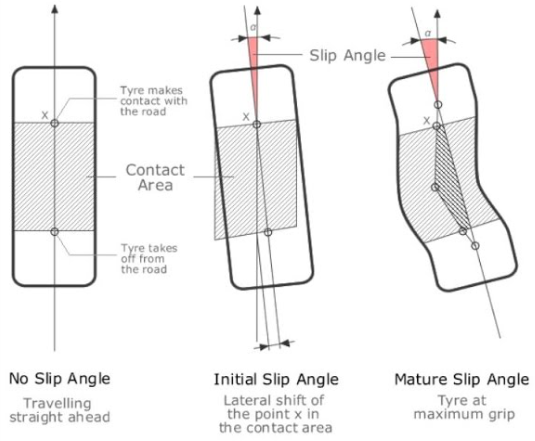
\includegraphics[width=\textwidth]{img/EA-angulo-deriva-neumatico.png}
		\caption{Deformación de la zona de contacto del neumático y ángulo de deriva~$\alpha$. Fuente: \parencite{iad_2026_deriva}.}
		\label{fig:angulo-deriva}
	\end{minipage}
	\hspace{0.05\textwidth}
	\begin{minipage}[b]{0.50\textwidth}
		\centering
		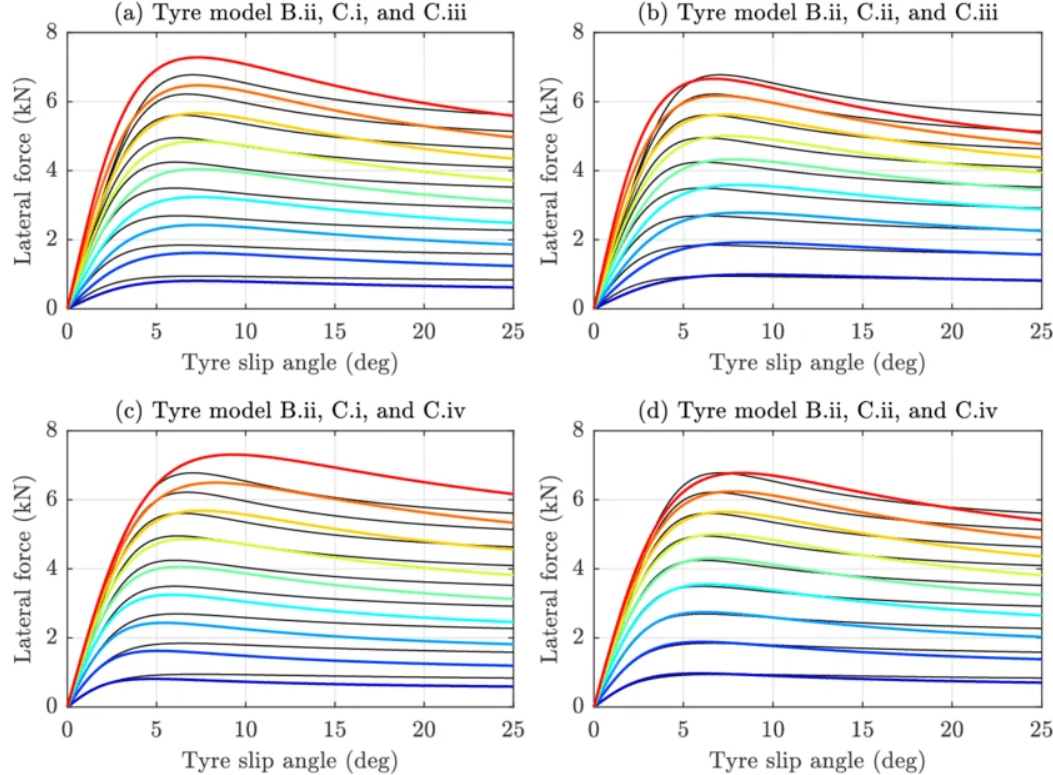
\includegraphics[width=\textwidth]{img/EA-formula-magica-neumatico.png}
		\caption{Fuerza lateral del neumático en función del ángulo de deriva para distintas cargas verticales (en color, modelos; en negro, datos medidos). Fuente: \parencite{sciencedirect_magic_formula}.}
		\label{fig:formula-magica}
	\end{minipage}
\end{figure}

\subparagraph{Vehículo.}
El resto del vehículo se divide en subsistemas: el motor y la transmisión, que entregan el par a las ruedas; la suspensión, que reparte las cargas entre ellas; la aerodinámica, que añade carga vertical en función de la velocidad; y los frenos. La transferencia de masas los relaciona entre sí: al frenar la carga se desplaza hacia el eje delantero, al acelerar hacia el trasero y en curva hacia las ruedas exteriores, de modo que el agarre disponible en cada neumático cambia constantemente según lo que haga el piloto.

Para que este modelo sea fiel, los desarrolladores trabajan con datos de coches reales, como planos CAD, medidas de suspensión, curvas de motor y datos aerodinámicos proporcionados por los fabricantes y equipos, además de cómo se comportan las ayudas electrónicas; estos datos son validados por pilotos que conducen dichos coches. Sobre este modelo se pueden modificar parámetros del vehículo para mejorar su rendimiento en los diferentes circuitos: altura y dureza de la suspensión, estabilizadores, ángulo de los alerones, presión de los neumáticos, relaciones de las marchas de la caja de cambios y reparto de frenada entre ejes. Cada cambio altera la física del coche y, con ella, su comportamiento y las fuerzas que llegan al volante.

Los simuladores más completos modelan además los daños y el desgaste mecánico. Un golpe puede deformar la suspensión o romper el alerón y desequilibrar el coche, los frenos pierden eficacia al sobrecalentarse y el motor o la caja de cambios pueden averiarse por un uso inadecuado.

Las figuras~\ref{fig:telemetria-motor} y~\ref{fig:telemetria-suspension} muestran algunas de estas magnitudes registradas durante una vuelta en el simulador.

\begin{figure}[H]   % H: justo aquí, debajo del subpárrafo «Vehículo»
	\centering
	% Mismo alto en las dos imágenes; el ancho de cada columna sigue la proporción de su captura
	\begin{minipage}[t]{0.478\textwidth}
		\centering
		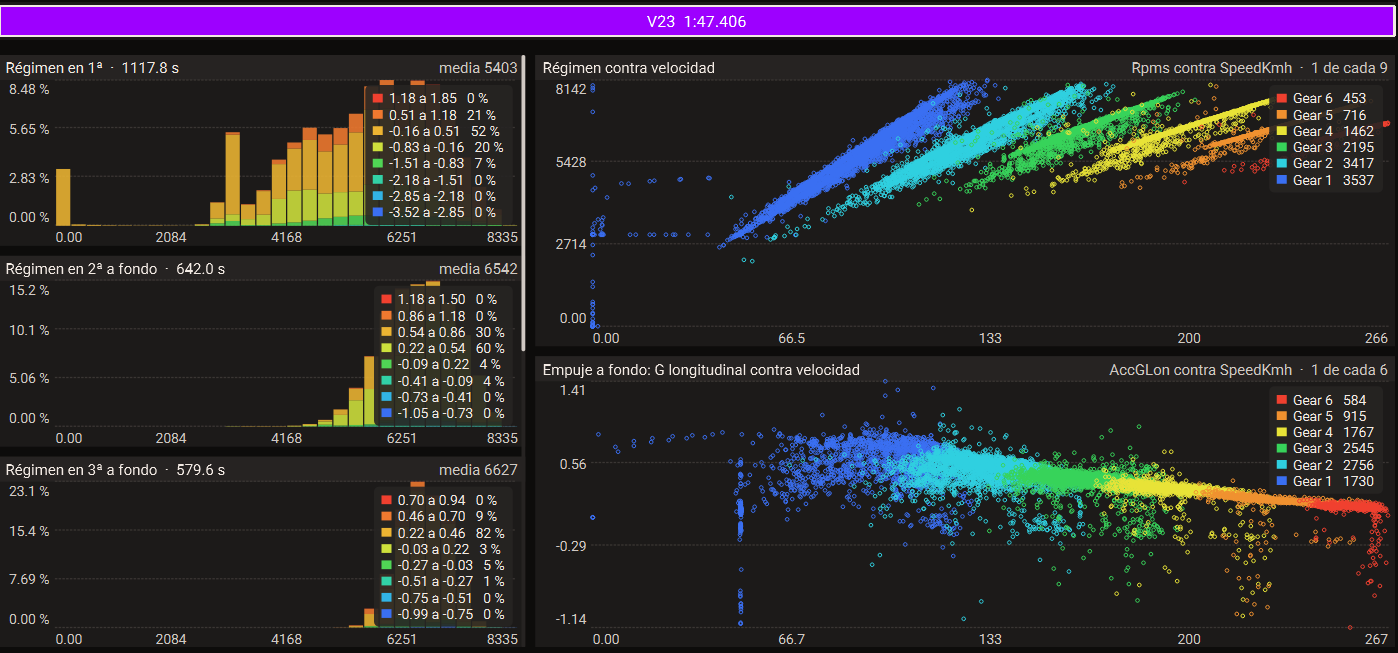
\includegraphics[width=\linewidth]{img/EA-rpmHisto.png}
		\caption[Telemetría del motor y la transmisión en una vuelta de simulador]{Motor y transmisión en una vuelta de 1:47,406. A la izquierda, el régimen en primera, segunda y tercera; a la derecha, régimen y aceleración longitudinal frente a la velocidad, un color por marcha: cada marcha forma su propia recta y muestra el escalonamiento de la caja de cambios.}
		\label{fig:telemetria-motor}
	\end{minipage}
	\hfill
	\begin{minipage}[t]{0.502\textwidth}
		\centering
		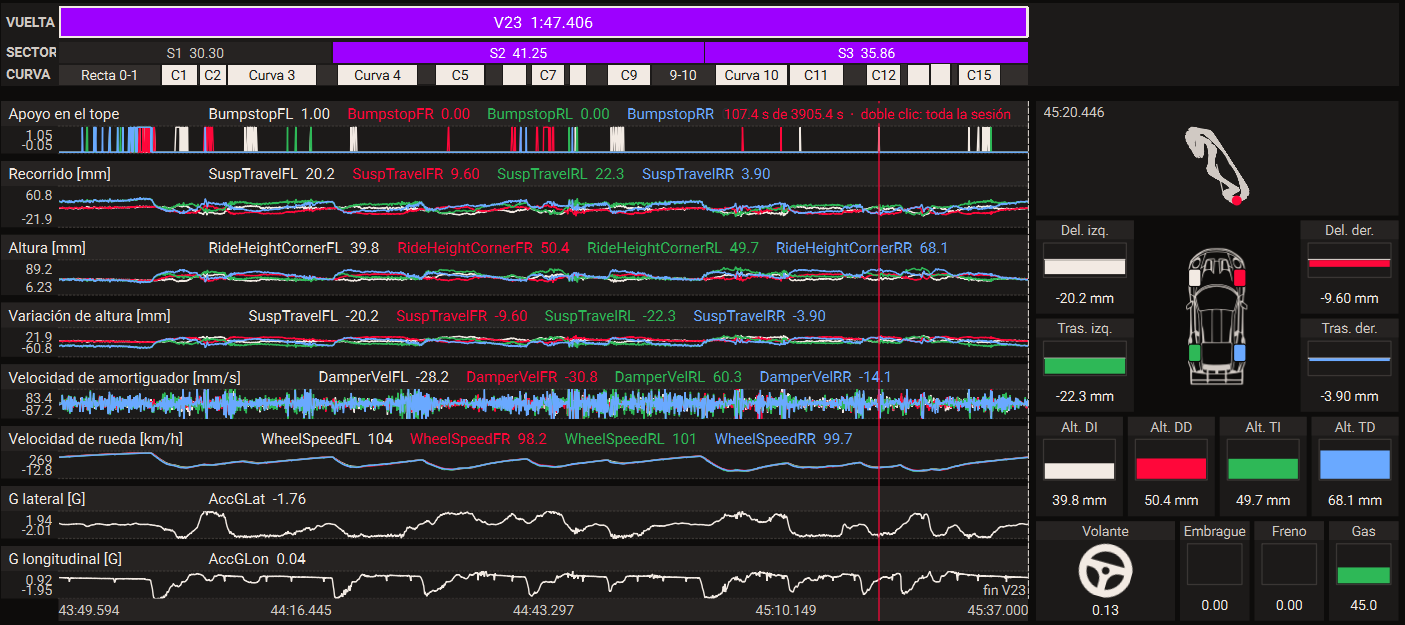
\includegraphics[width=\linewidth]{img/EA-suspensionHisto.png}
		\caption[Telemetría de la suspensión en una vuelta de simulador]{Suspensión en la misma vuelta, por sectores y curvas: tope, recorrido y altura de cada rueda, velocidad de los amortiguadores y de las ruedas, y aceleraciones lateral y longitudinal.}
		\label{fig:telemetria-suspension}
	\end{minipage}
	\par\medskip
	{\footnotesize Fuente de ambas figuras: capturas del analizador de telemetría del Configurador de VH SimGrid.}
\end{figure}

\subparagraph{Circuito.}
El modelo del coche se apoya en un modelo igual de detallado del circuito. Como se ha visto en la sección~\ref{sec:simracing-mercado}, los simuladores actuales reproducen los trazados a partir de escaneos láser del circuito real, con una precisión de milímetros que recoge los baches, los cambios de rasante, las variaciones de adherencia del asfalto y la forma exacta de los pianos. Estos detalles no son solo visuales: cada irregularidad de la superficie altera la carga de los neumáticos y, por tanto, las fuerzas que el piloto debe percibir a través del volante.

\paragraph{Frecuencia de cálculo y envío de datos.}
El modelo físico se resuelve en pasos discretos de tiempo, y la frecuencia con la que se hace condiciona la información que llega al piloto. Es importante diferenciar la frecuencia interna de la física y la frecuencia con la que el simulador envía la consigna a la base, que no coinciden siempre. iRacing es el caso más documentado: su física se resuelve internamente a 360~Hz, pero el cálculo del \textit{force feedback} y su envío al volante se hacen a 60~Hz, por lo que la base recibe un valor nuevo cada 16,7~ms \parencite{iracing_360hz}. Desde 2024 el simulador ofrece un modo de 360~Hz para las bases compatibles: en cada envío de 60~Hz incluye seis muestras, y es el firmware de la base el que las reproduce de forma escalonada. Este modo transmite señales de mayor frecuencia, como el golpe de un piano, a cambio de añadir un retraso de unos 16~ms \parencite{iracing_360hz}. rFactor~2, en cambio, lee la posición del volante y actualiza la salida de \textit{force feedback} a 400~Hz \parencite{overtake_ffb_analysis}.

Una frecuencia más alta no garantiza por sí sola una mejor sensación. Si el modelo físico completo no se calcula a esa velocidad, el simulador se limita a interpolar valores intermedios, y un modelo de neumático pobre no mejora por enviarse más a menudo \parencite{simxperience_ffb_myths}. Lo que sí se deduce de estas cifras es que la base debe trabajar a una frecuencia muy superior a la del simulador: entre dos consignas consecutivas tiene que mantener el par, suavizar la transición y responder por sí misma a los movimientos del piloto. Esta tarea, que se trata en la sección~\ref{sec:bases-ffb}, corresponde al firmware de la base y no al simulador.

\paragraph{Comunicación con los periféricos.}
En el ordenador, los periféricos de simracing se presentan como dispositivos USB de clase HID (\textit{Human Interface Device}), la misma que usan teclados, ratones y mandos. Esta clase permite al ordenador detectar estos dispositivos sin necesidad de controladores específicos: cada dispositivo describe en un descriptor qué ejes, botones y otros controles tiene, y el simulador los lee como si fueran un joystick. Las pedaleras, los aros y las botoneras se limitan a este papel de entrada y envían periódicamente la posición de sus ejes y el estado de sus botones.

Las bases, como se comentó anteriormente, no se limitan a enviar la posición actual del volante: también reciben información. Para ello la especificación HID incluye una extensión, la clase PID (\textit{Physical Interface Device}), que define cómo un programa  puede crear, modificar, iniciar y detener efectos de fuerza en un dispositivo \parencite{usb_hid_pid}. En Windows, los simuladores acceden a esta funcionalidad a través de la interfaz DirectInput, que agrupa los efectos en tres familias  \parencite{simracingcockpit_ffb}:
\begin{itemize}
	\item \textbf{Fuerza constante}: un par de valor y sentido determinados, que se actualiza cada vez que el simulador envía una nueva consigna. Es el efecto que usan los simuladores para transmitir la fuerza calculada en la dirección, y en la práctica el más importante.
	\item \textbf{Efectos periódicos}: señales con forma de onda (senoidal, cuadrada, triangular o diente de sierra) de amplitud y frecuencia configurables, que se emplean para vibraciones como las del motor o las de un piano.
	\item \textbf{Efectos condicionales}: fuerzas que dependen del estado del propio volante, como el muelle (proporcional al ángulo de giro), el amortiguador (proporcional a la velocidad), la fricción y la inercia (proporcional a la aceleración).
\end{itemize}

La diferencia entre las familias es relevante para el diseño de una base. La fuerza constante la calcula el simulador y la base solo tiene que reproducirla. Los efectos periódicos y condicionales, en cambio, se envían una sola vez con sus parámetros y es el firmware de la base el que los genera, leyendo su propio encoder a alta frecuencia. Una base compatible con el estándar debe implementar todos ellos, porque cada simulador usa una combinación distinta. Este es precisamente el papel de la capa de efectos HID de OpenFFBoard descrita en la sección~\ref{sec:soluciones-abiertas}.  

\paragraph{Telemetría.}
Los simuladores publican en tiempo real el estado completo de la sesión, como las revoluciones por minuto del motor, velocidad, estado de las suspensiones, tiempos por vuelta, temperatura y presión de los neumáticos, posición actual del piloto en la sesión y un largo conjunto de datos que cada simulador publica. Estos datos no se envían a los periféricos por la vía HID, sino que se ponen a disposición de otros programas del mismo ordenador. Los métodos más habituales son mediante memoria compartida y mediante el protocolo de comunicación UDP: Assetto Corsa Competizione, por ejemplo, usa la primera y la saga de Fórmula~1 de EA, la segunda \parencite{kunos_acc_shared_memory, ea_f1_25_udp}.

La telemetría es la fuente de información de todo lo que se muestra al piloto aparte del par en el volante como los LEDs, los \textit{dashes} con los datos del coche, los avisos de un ingeniero por voz o el análisis de las vueltas una vez terminada la sesión. Cada simulador la expone con un formato propio, por lo que cualquier programa que quiera usarla debe adaptarse a cada uno. Este problema, y las herramientas que lo resuelven, se tratan en la sección~\ref{sec:software-apoyo}.

\paragraph{Implicaciones para los periféricos.}
De lo anterior se desprenden los requisitos que el simulador impone al hardware. La base debe aceptar consignas de par por el protocolo HID PID, implementar los efectos estándar y trabajar a una frecuencia muy superior a la del simulador para reproducir la fuerza sin retrasos ni escalones. Los periféricos de entrada deben medir con suficiente resolución y frecuencia para que el modelo físico reciba las acciones del piloto tal como se producen. Y el conjunto debe poder aprovechar la telemetría para devolver al piloto la información que el par no transmite. Las siguientes subsecciones estudian cómo resuelve cada periférico estos requisitos.

\subsection{Bases de force feedback}
\label{sec:bases-ffb}

La base es el dispositivo que cierra el lazo en el sentido de la salida. Recibe del simulador la consigna del par calculada en la dirección del coche (sección~\ref{sec:simulacion-conduccion}) y la convierte en un par real en el eje del volante, que el piloto nota en las manos. Al mismo tiempo mide el ángulo de giro y lo devuelve al simulador como entrada. Todas las bases se componen de los mismos elementos: un motor eléctrico que genera el par, la transmisión que lo lleva hasta el eje, un sensor que mide la posición, una fuente de alimentación y un firmware que coordina el conjunto. Lo que diferencia una base de entrada de una profesional es cómo se resuelve cada uno de ellos.

\paragraph{Tipo de transmisión.}
La transmisión es el elemento que más condiciona el tacto de la base, y es el criterio con el que el mercado clasifica sus productos (sección~\ref{sec:mercado-perifericos}). Existen tres soluciones.

\subparagraph{Engranajes.}
Un motor de corriente continua pequeño y rápido mueve el eje del volante a través de un tren de engranajes que multiplica su par. Es la solución más barata y la de los volantes de entrada, como el Logitech~G29, que alcanza unos 2,2~N\,m \parencite{logitech_g29}. Sus inconvenientes son mecánicos. La holgura entre los dientes (\textit{backlash}) crea una pequeña zona muerta en la que el volante gira sin oponer resistencia, precisamente alrededor del centro, que es donde el piloto necesita más precisión. El paso de un diente a otro produce además un rizado que se nota como una textura granulosa, y el engranaje es ruidoso. Para disimular estos defectos, los fabricantes filtran la señal de \textit{force feedback}, y con ello se pierden los detalles más finos.

\subparagraph{Correa.}
El motor mueve el eje mediante una o varias correas dentadas y poleas de distinto diámetro. La correa elimina la holgura y el rizado de los engranajes, de modo que el tacto es mucho más suave y silencioso, y permite usar motores mayores, con pares de entre 4 y 8~N\,m. A cambio, la correa es elástica: se estira ligeramente bajo carga, lo que introduce un pequeño retraso y amortigua los cambios bruscos de fuerza. Además, el rozamiento de las poleas y la inercia del conjunto se suman a los del propio volante. Esta solución dominó la gama media antes de la llegada del \textit{direct drive}, y algunas bases combinan correa y engranajes en una transmisión híbrida, como el Thrustmaster~T150 \parencite{bsimracing_2015_t150}.

\subparagraph{Accionamiento directo (\textit{direct drive}).}
El volante se monta directamente sobre el eje del motor, sin ninguna reducción intermedia. Al no haber transmisión, desaparecen la holgura, el rizado, la elasticidad y el rozamiento añadidos: el par que genera el motor es exactamente el que llega a las manos del piloto, y cualquier detalle de la señal, por pequeño o rápido que sea, se transmite sin pérdidas. El precio de esta simplicidad es que el motor debe generar por sí solo todo el par, sin la multiplicación de una reducción. Por eso las bases \textit{direct drive} usan motores grandes y de alto par a baja velocidad, y necesitan una electrónica de control mucho más exigente. Hasta hace pocos años esto las limitaba a la gama profesional, pero hoy, como se ha visto, ofrecen desde unos 4~N\,m en la gama de entrada hasta 35~N\,m en la profesional \parencite{moza_web, simucube_web}.

La tabla~\ref{tab:transmisiones} resume las diferencias entre las tres soluciones.

\begin{table}[htbp]
	\centering
	\caption[Comparación de los tipos de transmisión de las bases de \textit{force feedback}]{Comparación de los tipos de transmisión de las bases de \textit{force feedback}. Adaptado de: \parencite{logitech_g29, moza_web, simucube_web}}
	\label{tab:transmisiones}
	\small
	\begin{tabular}{|l|c|c|c|}
		\hline
		\textbf{Característica} & \textbf{Engranajes} & \textbf{Correa} & \textbf{Direct drive} \\
		\hline
		Par típico (N\,m)       & 2--3       & 4--8       & 4--35 \\
		Holgura central         & Sí         & No         & No \\
		Rizado mecánico         & Alto       & Bajo       & Nulo \\
		Elasticidad / retraso   & Bajo       & Medio      & Nulo \\
		Ruido                   & Alto       & Bajo       & Muy bajo \\
		Detalle transmitido     & Bajo       & Medio      & Alto \\
		Coste                   & Bajo       & Medio      & Medio--alto \\
		\hline
	\end{tabular}
\end{table}

\paragraph{Motor.}
Las bases de engranajes y de correa usan motores de corriente continua con escobillas, sencillos de controlar: el par es proporcional a la corriente que circula por ellos, y basta con regular esa corriente. Las escobillas, sin embargo, se desgastan, producen rozamiento y limitan el par que el motor puede mantener.

Las bases \textit{direct drive} emplean motores síncronos de imanes permanentes sin escobillas, conocidos como  BLDC (\textit{Brushless DC}) o PMSM (\textit{Permanent Magnet Synchronous Motor}) según la forma de su fuerza contraelectromotriz \parencite{krishnan_2010_pmsm}. En ellos los imanes están en el rotor y los devanados en el estátor, de modo que no hay contactos que se desgasten y el calor se genera en la parte fija, donde es más fácil disiparlo. Para obtener mucho par a baja velocidad se usan motores de gran diámetro y muchos pares de polos, con una construcción similar a la de los motores de buje de bicicletas y patinetes eléctricos. Esta semejanza es la que aprovechan los proyectos de fabricación propia, y también este trabajo, para construir bases \textit{direct drive} a bajo coste.

Un defecto propio de estos motores es el \textit{cogging}: la atracción entre los imanes del rotor y los dientes del estátor crea unas posiciones preferentes en las que el rotor tiende a quedarse, y que se notan como pequeños escalones al girar el volante con la base sin par. Los fabricantes lo reducen con el diseño del motor, inclinando los imanes o las ranuras, o lo compensan desde el firmware midiendo su forma y aplicando un par opuesto \parencite{bianchi_2002_cogging, jahns_1996_torque_ripple, petrovic_2000_torque_ripple}.

\begin{figure}[htbp]
	\centering
	\captionsetup{justification=raggedright, singlelinecheck=false}   % columnas estrechas: pies sin justificar
	\begin{minipage}[b]{0.32\textwidth}
		\centering
		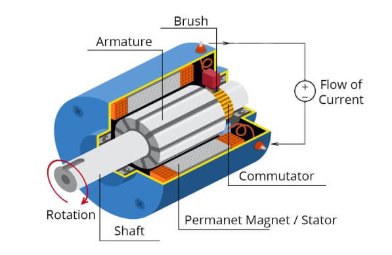
\includegraphics[width=\textwidth]{img/EA-motorDC.png}
		\caption[Motor de corriente continua con escobillas]{Motor de corriente continua con escobillas. Fuente: \parencite{salim_2025_brushed_dc}}
		\label{fig:motor-escobillas}
	\end{minipage}
	\hfill
	\begin{minipage}[b]{0.32\textwidth}
		\centering
		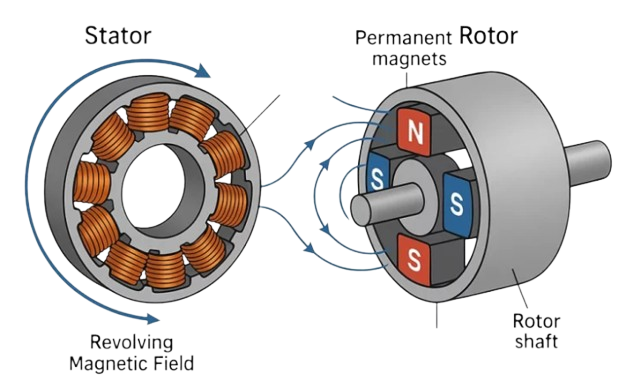
\includegraphics[width=\textwidth]{img/EA-motorBLDC.png}
		\caption[Motor sin escobillas de imanes permanentes (BLDC/PMSM)]{Motor sin escobillas de imanes permanentes (BLDC/PMSM). Fuente: \parencite{krishnan_2010_pmsm}}
		\label{fig:motor-bldc}
	\end{minipage}
	\hfill
	\begin{minipage}[b]{0.32\textwidth}
		\centering
		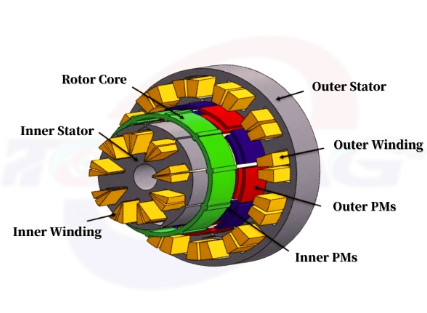
\includegraphics[width=\textwidth]{img/EA-motorPMSM.png}
		\caption[Motor de imanes permanentes de doble estátor]{Motor de imanes permanentes de doble estátor. Fuente: \parencite{wang_2011_double_stator}}
		\label{fig:motor-doble-estator}
	\end{minipage}
\end{figure}

\paragraph{El control vectorial (FOC).}
A diferencia del motor con escobillas, en un motor sin escobillas la corriente de cada fase debe conmutarse electrónicamente según la posición del rotor. La técnica que se usa en las bases de calidad es el control orientado al campo (\textit{Field Oriented Control}, FOC), también llamado control vectorial \parencite{krishnan_2010_pmsm}. Su idea es transformar las tres corrientes de fase, que son senoidales y dependen del ángulo del rotor, en dos componentes constantes referidas al propio rotor:
\begin{itemize}
	\item La corriente $i_q$ (en cuadratura), perpendicular al campo de los imanes, que es la que produce el par.
	\item La corriente $i_d$ (directa), alineada con el campo, que no produce par y que normalmente se mantiene en cero.
\end{itemize}
Este cambio de referencia se hace con dos transformaciones matemáticas, la de Clarke, que pasa de las tres fases a un sistema de dos ejes fijos, y la de Park, que gira ese sistema con el rotor usando el ángulo medido por el encoder. En el sistema resultante, el motor sin escobillas se comporta como uno de corriente continua, y el par es directamente proporcional a una sola corriente:
\begin{equation}
	T = k_t \, i_q
	\label{eq:par-foc}
\end{equation}
donde $k_t$ es la constante de par del motor, en N\,m/A. De este modo, convertir la consigna del simulador en par se reduce a controlar $i_q$ mediante un regulador PI, que compara la corriente medida con la deseada y ajusta la tensión aplicada a cada fase mediante modulación por ancho de pulso (PWM). Este lazo de corriente se ejecuta a varias decenas de kilohercios, cientos de veces más rápido que la consigna del simulador, y es el que garantiza que el par llega al volante sin rizado y sin retraso apreciable \parencite{briz_2000_current_regulators}. La ecuación~\ref{eq:par-foc} explica también por qué el FOC es imprescindible en el \textit{direct drive}: como no hay reducción que filtre las imperfecciones, cualquier error en el control de la corriente se nota directamente en las manos del piloto.

\paragraph{Medida de la posición.}
La base necesita conocer el ángulo del eje por dos motivos: el control FOC lo usa para orientar las corrientes en cada ciclo, y el simulador lo recibe como la posición del volante. Para ello se emplea un encoder, que puede ser de dos tipos según la tecnología:
\begin{itemize}
	\item \textbf{Ópticos}: un disco con ranuras gira entre un emisor de luz y un receptor, y cada ranura que pasa genera un pulso. Ofrecen alta resolución y no les afectan los campos magnéticos del motor.
	\item \textbf{Magnéticos}: un sensor mide la orientación de un imán solidario al eje. Son más baratos y compactos, pero su precisión depende de la alineación y pueden verse afectados por el campo del motor.
\end{itemize}
Además, el encoder puede ser incremental, que solo cuenta pulsos desde el arranque y necesita una referencia para conocer el centro, o absoluto, que conoce su posición en cuanto recibe alimentación. Su resolución determina la precisión con la que se mide el volante y la suavidad del control: en una base \textit{direct drive}, donde el giro del volante coincide con el del motor, un encoder de baja resolución se nota como pequeños escalones en el par.

\paragraph{Parámetros de una base.}
Más allá del tipo de transmisión, hay varios parámetros que definen las prestaciones de una base:
\begin{itemize}
	\item \textbf{Par máximo}: el par más alto que puede aplicar. Conviene distinguir entre el par de pico, que solo se mantiene unos instantes, y el par sostenido, que el motor aguanta sin sobrecalentarse. Un par elevado no se usa para que el volante sea más duro, sino para tener margen y reproducir sin saturar los golpes y los picos de fuerza.
	\item \textbf{Velocidad de respuesta} (\textit{slew rate}): la rapidez con la que el par puede cambiar, en N\,m/ms. Determina si la base reproduce fielmente los cambios bruscos, como un piano o una pérdida repentina de agarre.
	\item \textbf{Frecuencia de control}: la frecuencia del lazo de corriente y del procesamiento de efectos. Debe ser muy superior a la de la consigna del simulador para que la base pueda interpolar entre muestras y responder a los movimientos del piloto (sección~\ref{sec:simulacion-conduccion}).
	\item \textbf{Resolución del encoder}: cuentas por vuelta del sensor de posición.
	\item \textbf{Inercia y rozamiento propios}: los que añaden el rotor y la transmisión, que el piloto nota como un volante más pesado o más perezoso de lo que debería.
\end{itemize}

\paragraph{El firmware de la base.}
Entre la consigna del simulador y el lazo de corriente se sitúa el firmware de la base, que tiene tres funciones. La primera es atender la comunicación USB: presentarse como dispositivo HID, enviar el ángulo del volante e interpretar los efectos HID PID descritos en la sección~\ref{sec:simulacion-conduccion}, generando por sí mismo los efectos periódicos y condicionales.

La segunda es acondicionar la señal. Como la consigna llega a una frecuencia baja y en escalones, el firmware aplica un filtro de reconstrucción que suaviza la transición entre muestras. Además añade efectos propios que el usuario ajusta según su gusto: amortiguación, fricción e inercia simuladas, que dan cuerpo al volante y evitan oscilaciones, y limitadores de velocidad y de par. Estos ajustes son los que cada fabricante expone en su aplicación de configuración (sección~\ref{sec:soluciones-comerciales}).

La tercera es la seguridad. Una base \textit{direct drive} de gama media puede generar un par suficiente para lesionar la muñeca o el pulgar del piloto si el volante gira bruscamente, por ejemplo tras un choque en el simulador o por un error de comunicación. Por ello el firmware limita el par y la velocidad, corta la potencia si pierde la conexión con el ordenador, y las bases incluyen un pulsador de parada de emergencia que desconecta el motor de forma inmediata \parencite{simucube_safety}.

\paragraph{Implicaciones para el diseño.}
El análisis anterior explica por qué el mercado ha abandonado los engranajes y la correa en favor del \textit{direct drive}: es la única transmisión que no degrada la señal del simulador. También muestra dónde reside su dificultad, que no está en la mecánica, sino en el control del motor y en el firmware. Un motor sin escobillas de buje, una controladora FOC y un encoder de resolución suficiente son los mismos componentes que usan las bases comerciales, y están disponibles a bajo coste gracias a la robótica y a la movilidad eléctrica. Este es el planteamiento de la base de este trabajo, que combina un motor de patinete eléctrico, una controladora MKS ODrive Mini y un encoder óptico con un firmware propio que implementa el control FOC y el protocolo HID PID.

\subsection{Pedaleras}
\label{sec:pedaleras}
La pedalera se encarga de recoger las órdenes del piloto sobre el acelerador, el freno y el embrague. Estas órdenes se envían al simulador como ejes analógicos. Aunque parece el periférico más sencillo, es el que más influye en la regularidad del piloto, ya que de la frenada depende gran parte del tiempo por vuelta. Su calidad depende de qué magnitud se mide en cada pedal y qué mecanismo genera la resistencia que siente el pie.

\paragraph{Medir recorrido o medir fuerza.}
En un coche de competición, el pedal de freno apenas se desplaza: actúa sobre un circuito hidráulico
casi incompresible, de modo que lo que el piloto dosifica es la presión que ejerce, no la distancia que recorre el pie. En un monoplaza o un GT esa fuerza puede superar los 100~kg en una frenada fuerte: en la primera chicane de Monza, por ejemplo, los pilotos de Fórmula~1 aplicaron en 2025 unos 162~kg \parencite{brembo_2025_f1_numbers}. El piloto aprende a frenar por fuerza, con la memoria muscular de la pierna, y no por posición \parencite{segel_1970_pedal_force}.

Las pedaleras más básicas de la gama de entrada, sin embargo, miden el recorrido del pedal, ya que es la solución más sencilla y menos costosa. Esto obliga a frenar de una forma poco realista: el pie se desplaza mucho contra un muelle blando, y repetir el mismo punto de frenado resulta complicado. Por eso el salto de la gama de entrada a la media en las pedaleras es el paso de medir el recorrido a medir la fuerza en el freno, mientras que en el acelerador y el embrague, donde en el coche real sí importa la posición, basta con medir el recorrido.

\paragraph{Sensores de posición.}
Para medir el recorrido del acelerador y del embrague se usan dos tipos de sensor:
\begin{itemize}
	\item \textbf{Potenciómetros}: una resistencia variable cuyo cursor se desplaza con el pedal. Son
	baratos y sencillos, pero el contacto mecánico desgasta la pista resistiva con el uso, lo que
	provoca ruido en la señal, saltos en la lectura y zonas muertas que obligan a recalibrar.
	\item \textbf{Sensores de efecto Hall}: miden la variación del campo magnético de un imán solidario
	al pedal, sin contacto físico entre las piezas. Al no haber rozamiento no se desgastan, su lectura es
	estable a largo plazo y su resolución es mayor \parencite{ramsden_2006_hall}. Por estas ventajas han sustituido a los
	potenciómetros incluso en la gama de entrada, como en las CSL Pedals de Fanatec
	(sección~\ref{sec:soluciones-comerciales}).
\end{itemize}

\paragraph{Sensores de fuerza: la célula de carga.}
Para medir la fuerza en el freno se utiliza una célula de carga, que consiste en una pieza metálica a la que se adhieren galgas extensométricas, resistencias que cambian de valor al deformarse. Las galgas se conectan en un puente de Wheatstone, que convierte esa pequeña deformación en una diferencia de tensión proporcional a la fuerza aplicada \parencite{muller_2010_load_cells}. La señal es muy débil, del orden de milivoltios, por lo que necesita un amplificador y un conversor analógico-digital de alta resolución. En las pedaleras de fabricación propia es habitual el circuito HX711, que integra ambos con una resolución de 24~bits \parencite{hx711_datasheet}. Otra forma es la utilización de un amplificador de instrumentación analógico, como el INA333, cuya salida lee directamente el conversor del microcontrolador \parencite{ina333_datasheet}. Con este sistema, el pedal apenas se mueve y el simulador recibe la presión del pie, como en un coche real. 

La capacidad de la célula fija la fuerza máxima que puede medirse. Las pedaleras de gama media usan células de 100~kg y las de gama alta, de 200~kg o más, lo que permite reproducir las fuerzas de frenada
de un coche de competición (sección~\ref{sec:soluciones-comerciales}).

\begin{figure}[htbp]
	\centering
	\begin{minipage}[b]{0.64\textwidth}
		\centering
		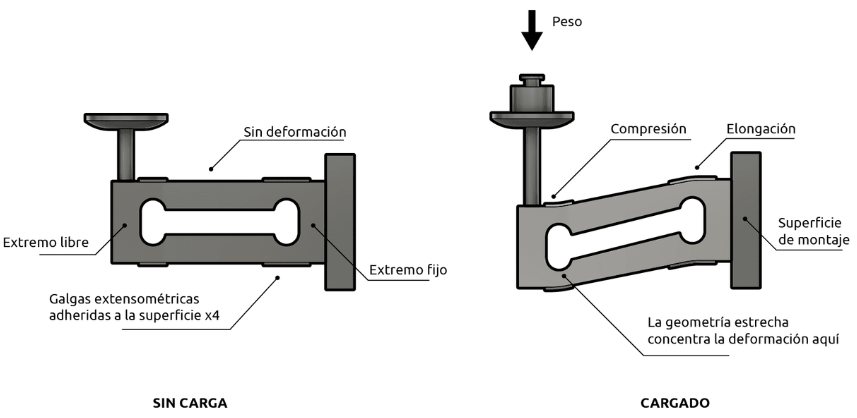
\includegraphics[width=\textwidth]{img/EA-celulaCarga.png}
		\caption[Funcionamiento de una célula de carga]{Funcionamiento de una célula de carga. Fuente: \parencite{muller_2010_load_cells}}
		\label{fig:celula-carga}
	\end{minipage}
\end{figure}

\paragraph{Resistencia y tacto del pedal.}
Medir la fuerza no basta, ya que el pedal debe oponer una resistencia que se parezca a la del coche real. Hay tres soluciones, de menor a mayor complejidad:
\begin{itemize}
	\item \textbf{Muelles y elastómeros}: el muelle da una resistencia lineal y el elastómero, una resistencia progresiva que se endurece al final del recorrido, como un circuito de freno real.
	Combinando muelles y elastómeros de distinta dureza se ajusta el tacto. Es la solución de la mayoría de las pedaleras con célula de carga.
	\item \textbf{Amortiguación hidráulica}: añade un amortiguador que reproduce la resistencia del líquido de frenos y suaviza la respuesta del pedal, como en las pedaleras de gama alta de Simagic o
	Heusinkveld.
	\item \textbf{Pedales activos}: un servomotor controlado por software genera la resistencia, lo que permite cambiar el tacto en cada coche y transmitir efectos como el ABS o el bloqueo de las ruedas. Es la tecnología de los pedales de Simucube y la más cara del mercado.
\end{itemize}

\paragraph{Retroalimentación háptica.}
Los pedales activos son la única solución que integra la resistencia y los efectos en el propio pedal, pero su precio los deja fuera del alcance de la mayoría. La alternativa es añadir a una pedalera pasiva
un actuador háptico que haga vibrar el pedal. El piloto no recibe la fuerza del coche, pero sí la información que más necesita en la frenada y la aceleración: la vibración en el freno indica que actúa
el ABS o que las ruedas se bloquean, y en el acelerador, que las ruedas traseras patinan. Se utilizan tres tipos de actuador \parencite{choi_2013_vibrotactile}:
\begin{itemize}
	\item \textbf{Motores de masa excéntrica (ERM)}: pequeños motores de corriente continua con una masa
	descentrada en el eje, como los de los mandos de consola. Son baratos y fáciles de controlar, pero tardan en arrancar y detenerse, y la frecuencia y la intensidad de la vibración están ligadas entre sí. Es la solución que incorporan, por ejemplo, el freno y el acelerador de las ClubSport Pedals~V3 de Fanatec \parencite{fanatec_web}.
	\item \textbf{Actuadores lineales}: un campo magnético desplaza una masa en línea recta, como en un altavoz. Responden más rápido y permiten controlar la frecuencia con independencia de la intensidad,
	lo que hace distinguible, por ejemplo, el ABS del paso por un piano. Es el principio del Haptic Pedal Reactor (P-HPR) de Simagic, que se monta detrás de la plataforma del pedal y alcanza hasta
	50~Hz \parencite{simagic_web}.
	\item \textbf{Transductores táctiles} (\textit{bass shakers}): actuadores de audio de baja frecuencia que se fijan al \textit{cockpit} o al asiento. Transmiten vibraciones a todo el puesto, como el motor o los baches, más que efectos concretos de un pedal.
\end{itemize}
Estos efectos no se calculan en la pedalera, sino a partir de la telemetría que publica el simulador. Programas como SimHub, mediante su módulo ShakeIt, leen esos datos y generan la señal de cada
actuador \parencite{simhub_web}. En las soluciones de fabricación propia, un microcontrolador recibe esa señal por USB y gobierna los motores mediante un controlador de potencia, lo que permite añadir vibración a una pedalera casera por muy poco coste.

\paragraph{Conexión y configuración.}
Sea cual sea el sensor, la pedalera se presenta al ordenador como un dispositivo USB HID con un eje por pedal, sin necesidad de controladores específicos. Sobre la lectura del sensor se aplican después ajustes por software: una calibración de los extremos, zonas muertas para evitar lecturas no deseadas en reposo y curvas de respuesta que modifican la relación entre la entrada del piloto y el valor enviado al simulador. Estos ajustes se realizan en el software de cada fabricante o, en las soluciones de fabricación propia, en el propio firmware del microcontrolador.
\subsection{Aros}
\label{sec:aros}

El aro es la parte del volante que el piloto sujeta y la única pieza del puesto que está en contacto permanente con sus manos. Cumple dos funciones: transmitir a las manos el par que genera la base y reunir los mandos que el piloto acciona sin soltar el volante. Por eso su diseño combina un componente mecánico, la forma, el tamaño y la rigidez del aro, con uno electrónico, los botones, levas y luces que lo convierten en un periférico de entrada.

\paragraph{Formatos.}
La forma del aro depende del tipo de coche que se quiere reproducir. Los aros redondos, de unos 300 a 350~mm de diámetro, corresponden a los turismos, los GT y los coches de rally, en los que el volante gira más de media vuelta y el piloto cambia la posición de las manos. Los aros de tipo Fórmula, más pequeños y con forma de mariposa, reproducen los de los monoplazas y los prototipos de resistencia: el giro es tan reducido que las manos no se mueven del aro, y casi todos los mandos del coche se concentran en él. Entre ambos se sitúan los aros de tipo GT con la parte superior abierta o plana, cada vez más habituales en los GT3 actuales, que combinan un giro amplio con una botonera completa, como el Podium Steering Wheel BMW~M4~GT3 de Fanatec \parencite{fanatec_web}.

\paragraph{Mandos.}
Un aro de competición reproduce los controles que el piloto usa durante la carrera. Los más sencillos son los pulsadores, que se asignan a funciones como el limitador de velocidad en el \textit{pit lane}, la radio o el cambio de página de la pantalla. Los selectores rotativos permiten ajustar parámetros por pasos, como el reparto de frenada, el control de tracción o el ABS, y los \textit{encoders} incrementales, que giran sin tope y envían un pulso por cada paso, se usan para recorrer menús o ajustar valores de forma continua. Detrás del aro se montan las levas de cambio y, en los aros de tipo Fórmula, dos levas analógicas de embrague que el piloto usa en las salidas para dosificar la tracción. Para detectar la posición de las levas se emplean microinterruptores, que dan un clic mecánico definido, o sensores Hall y magnéticos, que no se desgastan y permiten una lectura analógica \parencite{ramsden_2006_hall}.

\paragraph{Información al piloto.}
Además de recoger órdenes, el aro informa al piloto. La mayoría de los aros de gama media y alta incorpora una fila de LEDs que se encienden progresivamente con las revoluciones del motor e indican el momento del cambio de marcha, o dan información como las banderas en pista o el estado de la batería, según los gustos de cada piloto; los de gama alta añaden una pantalla con la marcha, los tiempos por vuelta o el estado de los neumáticos. Igual que la vibración de los pedales (sección~\ref{sec:pedaleras}), estos datos no los genera el aro, sino que proceden de la telemetría del simulador, leída por el software del fabricante o por programas como SimHub.

\paragraph{Electrónica.}
Un aro reúne fácilmente más de veinte entradas, demasiadas para conectar cada una a un pin del microcontrolador. La solución habitual es organizar los pulsadores en una matriz de filas y columnas, en la que el microcontrolador activa las filas una a una y lee las columnas para saber qué pulsador está pulsado. Con una matriz de 5$\times$5 se leen 25 pulsadores con solo 10 pines, y añadiendo un diodo en serie con cada pulsador se evitan las lecturas falsas cuando se pulsan varios a la vez. Los \textit{encoders} y las levas analógicas se leen aparte, y el microcontrolador presenta todo el conjunto al ordenador como un único dispositivo USB HID con botones y ejes, como permite la biblioteca Arduino Joystick sobre placas ATmega32U4 (sección~\ref{sec:soluciones-abiertas}).

\paragraph{Conexión con la base.}
El aro se une a la base mediante un anclaje rápido que transmite el par y, en los ecosistemas comerciales, también la alimentación y los datos a través de contactos eléctricos propios de cada marca. Como se vio en la sección~\ref{sec:productos-relacionados}, este es uno de los puntos en los que los fabricantes cierran su ecosistema: un aro de una marca solo funciona por completo sobre una base de la misma marca. La alternativa es separar ambas funciones: un anclaje puramente mecánico, compatible con el patrón de seis tornillos sobre un círculo de 70~mm habitual en los volantes de competición, y una conexión independiente del aro al ordenador por USB o por radio, como hacen Simucube y la mayoría de los aros de fabricación propia \parencite{simracingcockpit_qr, simucube_web}.

\paragraph{Materiales y fabricación.}
El aro debe ser rígido, porque cualquier flexión resta precisión a la información que llega de la base, y ligero, porque su inercia se suma a la que tiene que mover el motor. Los aros comerciales combinan una placa frontal de aluminio o fibra de carbono con empuñaduras de piel, ante o goma. En los aros de fabricación propia, la impresión 3D permite reproducir la forma y la disposición de mandos de un volante real a bajo coste, reservando las piezas metálicas para las zonas que soportan el par.

\subsection{Software de apoyo para el piloto}
\label{sec:software-apoyo}

Además del simulador y del software de configuración de cada fabricante, el piloto utiliza un conjunto de programas que le ayudan durante la carrera y después de ella. Ninguno modifica la física del simulador: todos trabajan sobre los datos que este publica, y cumplen funciones que en un equipo real reparten el ingeniero de pista, el \textit{spotter} y el analista de datos.

\paragraph{La telemetría como punto de partida.}
Todos estos programas dependen de la telemetría, el conjunto de datos que el simulador calcula en cada instante: velocidad, revoluciones, marcha, posición de los pedales y del volante, temperaturas y presiones de los neumáticos, combustible, posición en carrera o diferencias con los rivales. Los simuladores la ponen a disposición de otros programas de dos formas: escribiéndola en una zona de memoria compartida que cualquier aplicación del mismo ordenador puede leer, como hacen iRacing, Assetto Corsa Competizione o rFactor~2, o enviándola en paquetes UDP por la red, como la saga de Fórmula~1 o Gran Turismo~7, lo que permite leerla también desde otro dispositivo \parencite{kunos_acc_shared_memory, ea_f1_25_udp, gtplanet_gt7_telemetry}. Cada simulador usa además su propio formato, por lo que las herramientas de apoyo necesitan un adaptador para cada título.

\paragraph{Información en tiempo real.}
El primer grupo de programas muestra al piloto la información que necesita mientras conduce. La herramienta más extendida es SimHub, gratuita con una licencia opcional de pago, que reúne en una sola aplicación las pantallas de datos (\textit{dashes}), que pueden mostrarse en una pantalla auxiliar, en una tableta o superpuestas al juego, el control de los LEDs de revoluciones y banderas de aros y pantallas, y el módulo ShakeIt, que genera las vibraciones de pedales y asientos descritas en la sección~\ref{sec:pedaleras} \parencite{simhub_web}. Además, permite conectar placas Arduino para construir indicadores propios, lo que la ha convertido en la base de buena parte del hardware de fabricación propia. Z1 Dashboard cubre una función parecida, centrada en las pantallas y los LEDs \parencite{z1_web}.

\paragraph{Ingeniero y \textit{spotter} por voz.}
En una carrera real, el piloto recibe por radio la información que no puede leer mientras conduce. Crew Chief reproduce ese papel en el simulador: es una aplicación gratuita que actúa como ingeniero y como \textit{spotter}, avisa de los coches que se encuentran a los lados, de las banderas, de las diferencias con los rivales o del combustible restante, y con reconocimiento de voz permite preguntarle por esos datos sin soltar el volante. Funciona con la mayoría de los simuladores de PC, como iRacing, Assetto Corsa Competizione o rFactor~2 \parencite{crewchief_web}.

\paragraph{Análisis de telemetría.}
Después de la sesión, el piloto compara sus vueltas para encontrar dónde pierde tiempo, igual que hacen los ingenieros con los datos del coche real. Para ello se usan las mismas herramientas que en la competición profesional: Assetto Corsa Competizione exporta su telemetría en el formato de MoTeC~i2, el programa de análisis de datos más extendido en el automovilismo, e iRacing ofrece gratis a sus usuarios Pi Toolbox, el software de análisis de Cosworth, que lee directamente sus archivos \parencite{acc_motec_blog, motec_i2, cosworth_iracing}. Junto a ellas han surgido plataformas pensadas para el simracing, como Garage~61, que permite comparar las vueltas propias con las de otros pilotos en el mismo coche, o Coach Dave Delta, que además instala reglajes y señala automáticamente en qué curvas se pierde tiempo \parencite{garage61_web, coachdave_delta}.

\paragraph{Limitaciones.}
Estas herramientas cubren entre todas las necesidades del piloto, pero lo hacen por separado. Cada una tiene su propia instalación, su configuración y sus perfiles, y en un mismo puesto conviven a menudo SimHub, Crew Chief, un programa de análisis y el software de cada fabricante de periféricos. Ninguna conoce el hardware sobre el que se ejecuta: SimHub puede encender los LEDs de un aro, pero no ajusta el force feedback de la base ni la curva del freno, que siguen dependiendo de la aplicación de cada marca. Esta fragmentación es la que intenta resolver el configurador de este trabajo, que reúne en una sola aplicación las pantallas, las luces, el ingeniero por voz, la estrategia y el análisis de telemetría, y que conoce los periféricos a los que se conecta (sección~\ref{sec:estado-arte-conclusion}).
\section{Productos relacionados}
\label{sec:productos-relacionados}

El mercado de periféricos de simracing reúne hoy a un número creciente de fabricantes, con gamas que van desde equipos de entrada orientados al jugador ocasional hasta material profesional usado por pilotos y equipos de competición. Junto a esta oferta comercial ha crecido una comunidad de proyectos de código abierto y de fabricación propia (\textit{Do It Yourself}, DIY) que permite a un usuario construir sus propios periféricos a partir de controladoras de motor genéricas, microcontroladores y piezas impresas en 3D.

Esta sección analiza ambos enfoques. La sección~\ref{sec:mercado-perifericos} cuantifica el mercado y lo divide por gamas, la sección~\ref{sec:soluciones-comerciales} recoge las principales marcas comerciales (Fanatec, Simucube, Moza, Simagic y Heusinkveld) y la sección~\ref{sec:soluciones-abiertas}, las alternativas abiertas más extendidas (ODrive, OpenFFBoard, FFBeast y la biblioteca Arduino Joystick). Para que la comparación sea homogénea, cada solución se evalúa con los mismos criterios, derivados de los fundamentos técnicos de la sección~\ref{sec:fundamentos-tecnicos}:
\begin{itemize}
	\item \textbf{Transmisión y par}: tipo de transmisión de la base y par máximo disponible.
	\item \textbf{Medida en los pedales}: freno por recorrido o por fuerza, y tipo de sensor.
	\item \textbf{Apertura}: si el firmware y el diseño son abiertos o propietarios.
	\item \textbf{Ecosistema}: software de configuración, conexión entre aro y base, y compatibilidad con otras marcas.
	\item \textbf{Alcance}: qué periféricos cubre (base, aro, pedalera) y qué software de apoyo al piloto incluye.
	\item \textbf{Coste} aproximado.
\end{itemize}
El resultado se resume en la tabla~\ref{tab:comparativa}, que sirve de base para la conclusión del capítulo.

\subsection{Mercado de periféricos}
\label{sec:mercado-perifericos}

Cuantificar el mercado del simracing no es sencillo, porque los informes sectoriales no comparten una definición común. Los que se limitan a los simuladores de carreras, es decir, al hardware y al software de simulación, lo estiman en torno a 0,9~miles de millones de dólares en 2025, con un crecimiento anual del orden del 7--8\,\% \parencite{tbrc_2026_racing_sim}. Los que incluyen también los videojuegos de carreras en general elevan la cifra hasta unos 3,8~miles de millones de dólares en el mismo año, con previsiones que la sitúan cerca de los 7,7~miles de millones en 2035 \parencite{mri_2025_car_racing_games}. La diferencia entre ambas estimaciones confirma la distinción entre juegos y simuladores de la sección~\ref{sec:simracing-mercado}: el simracing, entendido como simulación con periféricos específicos, es una fracción del mercado de los juegos de carreras, pero una fracción con un gasto por usuario mucho mayor.

La figura~\ref{fig:mercado-estimaciones} compara las estimaciones de tres consultoras para el mercado de simuladores de carreras: aunque difieren en el punto de partida y en el horizonte, todas prevén que el mercado al menos se duplique en la próxima década.

% Estimaciones del mercado de simuladores de carreras según cada consultora (miles de millones de dólares).
% Datos y fuentes (valor de partida -> previsión):
%   MarketsandMarkets         0,50 (2024) -> 1,10 (2030)
%   Mordor Intelligence       0,98 (2025) -> 2,04 (2030)
%   Market Research Future    1,05 (2025) -> 4,31 (2035)
\begin{figure}[htbp]
	\centering
	\begin{tikzpicture}
		\begin{axis}[
			grafica,
			scale only axis, width=0.5\linewidth, height=5.5cm,
			xbar=3pt, bar width=8pt,
			xmin=0, xmax=5.2,
			area legend,
			legend style={/tikz/every even column/.append style={column sep=10pt}},
			xmajorgrids, ymajorgrids=false,
			axis lines*=left,
			symbolic y coords={Market Research Future,Mordor Intelligence,MarketsandMarkets},
			ytick=data,
			y dir=reverse,
			enlarge y limits=0.15,
			xlabel={Tamaño del mercado (miles de millones de dólares)},
			point meta=explicit symbolic,
			nodes near coords,
			every node near coord/.append style={font=\scriptsize, text=black, anchor=west},
			legend style={at={(0.5,1.02)}, anchor=south},
		]
			\addplot[fill=serie1, draw=none] coordinates {
				(0.50,MarketsandMarkets) [0,50 (2024)]
				(0.98,Mordor Intelligence) [0,98 (2025)]
				(1.05,Market Research Future) [1,05 (2025)]
			};
			\addplot[fill=serie2, draw=none] coordinates {
				(1.10,MarketsandMarkets) [1,10 (2030)]
				(2.04,Mordor Intelligence) [2,04 (2030)]
				(4.31,Market Research Future) [4,31 (2035)]
			};
			\legend{Valor de partida, Previsión}
		\end{axis}
	\end{tikzpicture}
	\caption[Estimaciones del mercado de simuladores de carreras]{Estimaciones del tamaño del mercado de simuladores de carreras según tres consultoras, con el año de cada valor. Fuente: resúmenes públicos de los informes de MarketsandMarkets, Mordor Intelligence y Market Research Future \parencite{marketsandmarkets_racing_sim, mordor_2025_racing_sim, mrfr_2025_racing_sim}.}
	\label{fig:mercado-estimaciones}
\end{figure}


Coinciden, en cambio, en los factores que explican el crecimiento: la popularidad de los eSports, la implicación de pilotos y equipos profesionales y la mejora del hardware disponible para el consumidor \parencite{mordor_2025_racing_sim}. Este último factor es el más relevante para este trabajo. La llegada de las bases \textit{direct drive} y de las pedaleras con célula de carga a precios de consumo (sección~\ref{sec:soluciones-comerciales}) ha hecho que el periférico sea el componente que más pesa en el coste de un ecosistema propio: un aficionado puede pagar una suscripción mensual o simuladores por decenas de euros, pero un ecosistema completamente equipado con base, aro y pedalera de gama media supera con facilidad los mil euros.

La evolución de Fanatec, el mayor fabricante del sector, ilustra este auge del hardware (figura~\ref{fig:fanatec-facturacion}): su facturación se multiplicó por más de diez entre 2016 y 2022, con un salto del 132\,\% en 2020.

% Facturación anual de Endor AG, empresa propietaria de Fanatec (millones de euros).
% Datos y fuentes:
%   2016-2021  Börsengeflüster, "Endor: Voll auf Wachstumskurs" (tabla de Umsatzerlöse)
%   2020       Endor AG, cifras preliminares 2020: 90 M€ frente a 38,8 M€ en 2019 (+132 %)
%   2021       Endor AG, cifras preliminares 2021: un 10 % menos por falta de suministro
%   2022       TraderFox (119,19 M€); Landshuter Rundschau cita 119 M€
\begin{figure}[htbp]
	\centering
	\begin{tikzpicture}
		\begin{axis}[
			grafica,
			ybar, bar width=18pt,
			ymin=0, ymax=135,
			xtick=data,
			xticklabel style={/pgf/number format/1000 sep={}},
			ylabel={Facturación (millones de euros)},
			nodes near coords,
			every node near coord/.append style={font=\footnotesize, text=black,
				/pgf/number format/fixed, /pgf/number format/precision=1},
			enlarge x limits=0.08,
		]
			\addplot[fill=serie1, draw=none]
				coordinates {
					(2016, 10.2) (2017, 18.4) (2018, 22.1) (2019, 38.8)
					(2020, 90.2) (2021, 81.3) (2022, 119.2)
				};
		\end{axis}
	\end{tikzpicture}
	\caption[Facturación anual de Endor AG (Fanatec)]{Facturación anual de Endor AG, la empresa propietaria de Fanatec, entre 2016 y 2022. El salto de 2020 coincide con la pandemia y la caída de 2021 se debe a la falta de suministro de componentes. Fuente: comunicados de resultados de Endor AG \parencite{endor_web}.}
	\label{fig:fanatec-facturacion}
\end{figure}


\paragraph{Segmentación del mercado de periféricos.}
De lo anterior se desprende una segmentación por niveles que se mantiene en el resto de la sección:
\begin{itemize}
	\item \textbf{Gama de entrada}: volantes con transmisión por engranajes o correa y pedales que miden el recorrido, pensados para el jugador ocasional y compatibles con consolas.
	\item \textbf{Gama media}: bases \textit{direct drive} de bajo y medio par y pedaleras con célula de carga, donde se concentra hoy el crecimiento del sector.
	\item \textbf{Gama alta y profesional}: bases de alto par, pedales hidráulicos o activos, réplicas de volantes reales y simuladores completos con plataformas de movimiento, usados por equipos, academias y pilotos profesionales.
\end{itemize}
El salto entre la gama de entrada y la media es el más significativo tanto en experiencia como en precio, y es el espacio en el que se sitúa la propuesta de este trabajo.

\subsection{Productos comerciales}
\label{sec:soluciones-comerciales}

La oferta comercial se concentra en pocos fabricantes, que en los últimos años han llevado el \textit{direct drive} de la gama profesional a la de entrada. Los cinco que se analizan cubren todo el espectro de precios y los dos modelos de negocio dominantes: el ecosistema completo, en el que una misma marca vende base, aros y pedaleras, y el fabricante especializado en un solo tipo de periférico.

\paragraph{Fanatec.}
Fanatec, la marca de simracing de la alemana Endor~AG, ha sido durante años el fabricante de mayor volumen del sector, con unas ventas cercanas a los 110 millones de dólares en 2023. En 2024, dentro del procedimiento de insolvencia de Endor, la compró Corsair, y hoy forma parte de un grupo de periféricos para videojuegos \parencite{businesswire_2024_corsair_fanatec}.

\textit{Colaboraciones con marcas reales.} Fanatec ha construido su imagen sobre licencias del mundo del motor: colabora con Porsche desde 2006 y con BMW desde 2011. El caso más relevante es el Podium Steering Wheel BMW~M4~GT3 (2022), que no es una réplica: Fanatec y BMW M Motorsport lo desarrollaron, con pilotos oficiales como Philipp Eng, para el propio coche de competición, y la versión de simulación es el mismo volante, con los mismos mandos y el mismo tacto que el piloto encuentra en pista \parencite{fanatec_web}. Desde 2018 es además socio de las F1 Esports Series, lo que le permite vender aros con licencia de la Fórmula~1 \parencite{fanatec_web}.

\textit{Bases.} Todo el catálogo es \textit{direct drive} y comparte el anclaje rápido QR2. La gama se escalona por par, desde la CSL~DD (5~N\,m, ampliable a 8~N\,m) hasta la Podium~DD (25~N\,m sostenidos y picos de 33~N\,m), que en 2026 sustituyó a la Podium~DD2 \parencite{fanatec_web}. Tras la bajada de precios de principios de 2026, la gama va de unos 330 a 1\,100~euros (tabla~\ref{tab:fanatec}).

\begin{table}[htbp]
	\centering
	\caption[Bases \textit{direct drive} de Fanatec (precios oficiales en euros, 2026)]{Bases \textit{direct drive} de Fanatec (precios oficiales en euros, 2026). Fuente: \parencite{fanatec_web}}
	\label{tab:fanatec}
	\begin{tabular}{|l|c|c|l|}
		\hline
		\textbf{Base} & \textbf{Par (N\,m)} & \textbf{Precio (\euro)} & \textbf{Plataformas} \\
		\hline
		CSL DD        & 5 (8 con kit) & 329,95    & PC, Xbox \\
		GT DD Pro     & 8             & 499,95    & PC, PlayStation \\
		ClubSport DD  & 12            & 599,95    & PC \\
		ClubSport DD+ & 15            & 799,95    & PC, PlayStation \\
		Podium DD     & 25 (33 pico)  & 1\,099,95 & PC, Xbox \\
		\hline
	\end{tabular}
\end{table}

\textit{Pedaleras.} Las CSL Pedals de entrada miden el freno por recorrido, aunque con sensores Hall sin contacto en lugar de potenciómetros, y admiten un kit de célula de carga. La célula viene de serie en las gamas superiores: las ClubSport Pedals~V3 miden hasta 90~kg y las Podium Pedals, de 2026, hasta 150~kg en el pedal \parencite{fanatec_web}. Como en las bases, el sensor y la fuerza máxima marcan la diferencia entre gamas (tabla~\ref{tab:fanatec-pedales}).

\begin{table}[htbp]
	\centering
	\caption[Pedaleras de Fanatec (precios oficiales en euros, 2026)]{Pedaleras de Fanatec (precios oficiales en euros, 2026). Fuente: \parencite{fanatec_web}}
	\label{tab:fanatec-pedales}
	\small
	\begin{tabular}{|l|l|c|c|}
		\hline
		\textbf{Pedalera} & \textbf{Sensor del freno} & \textbf{Fuerza máx. (kg)} & \textbf{Precio (\euro)} \\
		\hline
		CSL Pedals                        & Hall (por recorrido) & --  & 99,95 \\
		CSL Pedals LC                     & Célula de carga      & --  & 179,90 \\
		CSL Elite Pedals V2               & Célula de carga      & --  & 299,95 \\
		ClubSport Pedals V3               & Célula de carga      & 90  & 329,95 \\
		ClubSport Pedals V3 Inverted      & Célula de carga      & 90  & 429,99 \\
		Podium Pedals Sport (2 pedales)   & Célula de carga      & 150 & 599,95 \\
		Podium Pedals Formula (2 pedales) & Célula de carga      & 150 & 699,95 \\
		\hline
	\end{tabular}
\end{table}

\textit{Aros y ecosistema.} Los aros muestran el peso de las licencias en el precio (tabla~\ref{tab:fanatec-aros}): los de estilo GT o Fórmula cuestan entre 200 y 360~euros, mientras que el BMW~M4~GT3, que procede del coche real, ronda los 1\,500, más que la base más potente de la marca. Todos se conectan por el QR2, que lleva la alimentación y los datos del aro, y se configuran desde la aplicación de Fanatec. Es el ecosistema más completo del mercado y también el más cerrado, y su principal ventaja es la compatibilidad oficial con consolas, poco habitual en el resto de marcas.

\begin{table}[htbp]
	\centering
	\caption[Selección de aros de Fanatec (precios oficiales en euros, 2026)]{Selección de aros de Fanatec (precios oficiales en euros, 2026). Fuente: \parencite{fanatec_web}}
	\label{tab:fanatec-aros}
	\small
	\begin{tabular}{|l|l|l|c|}
		\hline
		\textbf{Aro} & \textbf{Estilo} & \textbf{Licencia} & \textbf{Precio (\euro)} \\
		\hline
		CSL Steering Wheel GT3                     & GT      & --        & 199,95 \\
		ClubSport Steering Wheel F1 Esports V2     & Fórmula & Formula 1 & 239,95 \\
		CSL Elite Steering Wheel Porsche Vision GT & GT      & Porsche   & 349,95 \\
		ClubSport Steering Wheel Formula V2.5      & Fórmula & --        & 359,95 \\
		Podium Steering Wheel BMW M4 GT3           & GT      & BMW M Motorsport\textsuperscript{*} & 1\,499,95 \\
		\hline
		\multicolumn{4}{l}{\footnotesize \textsuperscript{*} Volante desarrollado para el coche de competición real.} \\
	\end{tabular}
\end{table}



\paragraph{Simucube.}
Simucube nace de Granite Devices, una empresa finlandesa de servoaccionamientos industriales. En 2016 lanzó por micromecenazgo el SimuCUBE~1, una controladora de force feedback surgida de la comunidad de simracing de fabricación propia, y con la Simucube~2, en 2019, pasó a dedicarse por completo a la simulación \parencite{simucube_web}. Es el único fabricante analizado que procede del control industrial de motores, y su prestigio se apoya en la calidad de ese control.

\textit{Colaboraciones con equipos reales.} En lugar de licencias de fabricantes, Simucube se apoya en alianzas con equipos: es socio oficial de Verstappen Sim Racing, cuyos pilotos usan solo su material, y mantiene un acuerdo técnico con Rodin Motorsport, que emplea sus productos en su simulador \textit{driver-in-the-loop} y en la preparación de sus pilotos \parencite{simucube_web}.

\textit{Bases.} La Simucube~2, durante años la referencia de la gama alta, ha dado paso a la Simucube~3, cuyos pedidos se abrieron en octubre de 2025. Estrena motor y se ofrece en Sport (15~N\,m), Pro (25~N\,m) y Ultimate (35~N\,m), el par más alto de los fabricantes analizados \parencite{simucube_web}. También es la más cara: la Pro cuesta unos 1\,490~euros, frente a los 1\,100 de la Podium~DD de Fanatec con el mismo par, y la Ultimate supera los 3\,200 (tabla~\ref{tab:simucube}).

\begin{table}[htbp]
	\centering
	\caption[Bases \textit{direct drive} de Simucube (precios oficiales en euros, 2026)]{Bases \textit{direct drive} de Simucube (precios oficiales en euros, 2026). Fuente: \parencite{simucube_web}}
	\label{tab:simucube}
	\small
	\begin{tabular}{|l|c|c|l|}
		\hline
		\textbf{Base} & \textbf{Par (N\,m)} & \textbf{Precio (\euro)} & \textbf{Estado} \\
		\hline
		Simucube 3 Sport    & 15 & 1\,246,80 & Actual \\
		Simucube 3 Pro      & 25 & 1\,486,80 & Actual \\
		Simucube 3 Ultimate & 35 & 3\,214,80 & Actual \\
		Simucube 2 Sport    & 17 & --        & Retirada \\
		Simucube 2 Pro      & 25 & --        & Retirada \\
		Simucube 2 Ultimate & 32 & --        & Retirada \\
		\hline
	\end{tabular}
\end{table}

\textit{Pedaleras.} En lugar de pedaleras convencionales fabrica pedales activos: en el ActivePedal la resistencia la genera un servomotor controlado por software, lo que permite cambiar la dureza y la curva en cada coche y transmitir efectos como el ABS o el bloqueo de la rueda. Es el principio del force feedback aplicado al pedal. Cada pedal cuesta entre unos 1\,090 y 2\,500~euros según la versión \parencite{simucube_web}, más que muchas bases \textit{direct drive} completas (tabla~\ref{tab:simucube-otros}).

\textit{Aros y ecosistema.} Sus aros, como el Tahko~GT-21 o el Savu Pro, son inalámbricos: el anclaje rápido es solo mecánico y el aro se comunica con la base por radio, lo que también facilita montar aros de terceros conectados por USB. Todo se configura con Simucube Tuner, y la marca no ofrece compatibilidad con consolas.

\begin{table}[htbp]
	\centering
	\caption[Pedales y aros de Simucube (precios en euros, 2026)]{Pedales y aros de Simucube (precios en euros, 2026). Fuente: \parencite{simucube_web}}
	\label{tab:simucube-otros}
	\small
	\begin{tabular}{|l|l|c|}
		\hline
		\textbf{Producto} & \textbf{Tipo} & \textbf{Precio (\euro)} \\
		\hline
		ActivePedal Sport        & Pedal activo (servomotor) & 1\,089,99 \\
		ActivePedal Pro          & Pedal activo (servomotor) & $\approx$\,1\,760 \\
		ActivePedal Ultimate     & Pedal activo (servomotor) & $\approx$\,2\,500 \\
		Tahko GT-21              & Aro GT inalámbrico        & 829,99 \\
		Savu Pro                 & Aro Fórmula inalámbrico   & desde 1\,259,99 \\
		\hline
		\multicolumn{3}{l}{\footnotesize Precio de los pedales por unidad.} \\
	\end{tabular}
\end{table}

\paragraph{Moza.}
Moza Racing es la división de simracing de Gudsen Technology, una empresa de Shenzhen fundada en 2012 y conocida por sus estabilizadores de cámara (\textit{gimbals}). En 2021 llevó su experiencia en control de motores a la simulación con un ecosistema \textit{direct drive} completo \parencite{moza_web}, y en cinco años se ha convertido en el principal competidor de Fanatec gracias a sus precios.

\textit{Colaboraciones con marcas reales.} Como Fanatec, apuesta por las licencias: vende aros oficiales de Lamborghini y de Porsche, cuyo Mission~R se reprodujo a partir de los datos CAD del fabricante, y en la Gamescom de 2026 presentó otros de Porsche, Mercedes-Benz y Ford. Desde agosto de 2026 es además socio oficial de la Gran Turismo World Series \parencite{moza_web}.

\textit{Bases.} Tiene la escalera de par más fina del mercado, con una base cada 3 o 4~N\,m desde la R3 (3,9~N\,m) hasta la R25 Ultra, y los precios más bajos de los fabricantes analizados: la R16 Ultra cuesta unos 550~euros, menos que la ClubSport~DD de Fanatec de 12~N\,m \parencite{moza_web} (tabla~\ref{tab:moza}).

\begin{table}[htbp]
	\centering
	\caption[Bases \textit{direct drive} de Moza (precios oficiales, 2026)]{Bases \textit{direct drive} de Moza (precios oficiales, 2026). Fuente: \parencite{moza_web}}
	\label{tab:moza}
	\small
	\begin{tabular}{|l|c|c|}
		\hline
		\textbf{Base} & \textbf{Par (N\,m)} & \textbf{Precio} \\
		\hline
		R3 (pack con aro y pedales)  & 3,9 & 399~\$ \\
		R5 Pro (pack)                & 6   & 419~\euro \\
		R9 V3                        & 9   & 399~\euro \\
		R12 V2                       & 12  & 529~\euro \\
		R16 Ultra                    & 16  & 549~\euro \\
		R21 Ultra                    & 21  & 699~\$ \\
		R25 Ultra                    & --  & 899~\$ \\
		\hline
		\multicolumn{3}{l}{\footnotesize En dólares cuando no hay precio oficial en euros.} \\
	\end{tabular}
\end{table}

\textit{Pedaleras.} La SR-P de entrada usa un sensor de fuerza de 100~kg en el freno, y la CRP2 de gama alta una célula de carga de 200~kg, comparable a la de las Podium Pedals de Fanatec, que cuestan unos 250~euros más \parencite{moza_web} (tabla~\ref{tab:moza-pedales-aros}).

\textit{Aros y ecosistema.} Combina aros propios, de unos 280 a 830~euros, con los licenciados, que llegan a los 1\,299~dólares del Porsche Mission~R. Como en Fanatec, el anclaje rápido lleva la conexión eléctrica del aro, así que los aros Moza solo funcionan completos sobre bases Moza, y todo se configura desde su aplicación Pit House.

\begin{table}[htbp]
	\centering
	\caption[Pedaleras y aros de Moza (precios oficiales, 2026)]{Pedaleras y aros de Moza (precios oficiales, 2026). Fuente: \parencite{moza_web}}
	\label{tab:moza-pedales-aros}
	\small
	\begin{tabular}{|l|l|l|c|}
		\hline
		\textbf{Producto} & \textbf{Tipo} & \textbf{Licencia / sensor} & \textbf{Precio} \\
		\hline
		SR-P               & Pedalera     & Sensor de 100 kg        & 159~\euro \\
		CRP2               & Pedalera     & Célula de carga 200 kg  & 449~\euro \\
		KS                 & Aro GT       & --                      & 279~\euro \\
		GS V2P             & Aro GT       & --                      & 439~\euro \\
		FSR2               & Aro Fórmula  & --                      & 699~\euro \\
		Vision GS          & Aro GT       & --                      & 829~\euro \\
		Lamborghini Revuelto & Aro GT     & Lamborghini             & 399~\$ \\
		Porsche Mission R  & Aro GT       & Porsche                 & 1\,299~\$ \\
		\hline
	\end{tabular}
\end{table}

\paragraph{Simagic.}
Simagic es un fabricante chino de gama media-alta, con buena relación calidad-precio, que hasta 2026 prefirió asociarse con competiciones y pilotos antes que con fabricantes de automóviles.

\textit{Colaboraciones con marcas reales.} Desde 2023 es proveedor oficial de la Formula DRIFT, el campeonato estadounidense de drift, con cuyos pilotos ha calibrado su force feedback, y en 2026 renovó el acuerdo por varios años. En octubre de 2026 anunció su primer volante licenciado, el del Aston Martin Valkyrie, al que seguirá el del KTM X-Bow~GT2 \parencite{simagic_web}.

\textit{Bases.} La familia Alpha EVO va de la Sport (9~N\,m) a la Ultra (28~N\,m), por entre unos 400 y 970~euros \parencite{simagic_web}. Por par y precio se sitúa entre Moza y Fanatec: la Ultra ofrece más par que la Podium~DD por unos 130~euros menos (tabla~\ref{tab:simagic}).

\begin{table}[htbp]
	\centering
	\caption[Bases \textit{direct drive} de Simagic (precios en euros de distribuidor europeo, 2026)]{Bases \textit{direct drive} de Simagic (precios en euros de distribuidor europeo, 2026). Fuente: \parencite{simagic_web}}
	\label{tab:simagic}
	\small
	\begin{tabular}{|l|c|c|}
		\hline
		\textbf{Base} & \textbf{Par (N\,m)} & \textbf{Precio (\euro)} \\
		\hline
		Alpha EVO Sport & 9  & 396,69 \\
		Alpha EVO       & 12 & 553,71 \\
		Alpha EVO Pro   & 18 & 702,47 \\
		Alpha EVO Ultra & 28 & 966,93 \\
		\hline
	\end{tabular}
\end{table}

\textit{Pedaleras.} La P1000 es modular, con una célula de carga de 100~kg en el freno que puede cambiarse por un sensor Hall, y la P2000 añade un sistema hidráulico que reproduce el tacto de un circuito de freno real, con células de 100 o 200~kg \parencite{simagic_web}. Es la única marca que lleva el freno hidráulico a la gama media (tabla~\ref{tab:simagic-pedales-aros}).

\textit{Aros y ecosistema.} Sus aros propios van de unos 300 a más de 500~euros, y el Aston Martin Valkyrie cuesta 799~dólares. Como el resto, usa un anclaje y un protocolo propios y se configura con su aplicación SimPro Manager.

\begin{table}[htbp]
	\centering
	\caption[Pedaleras y aros de Simagic (precios de 2026)]{Pedaleras y aros de Simagic (precios de 2026). Fuente: \parencite{simagic_web}}
	\label{tab:simagic-pedales-aros}
	\small
	\begin{tabular}{|l|l|l|c|}
		\hline
		\textbf{Producto} & \textbf{Tipo} & \textbf{Licencia / sensor} & \textbf{Precio} \\
		\hline
		P1000 (3 pedales)        & Pedalera     & Célula de carga 100 kg       & 469~\$ \\
		P2000 (3 pedales)        & Pedalera     & Hidráulica, célula de 200 kg & 689~\$ \\
		GT Neo                   & Aro GT       & --                           & $\approx$\,300~\euro \\
		FX Pro V2                & Aro Fórmula  & --                           & 549~\euro\textsuperscript{*} \\
		Aston Martin Valkyrie    & Aro GT       & Aston Martin                 & 799~\$ \\
		\hline
		\multicolumn{4}{l}{\footnotesize \textsuperscript{*} Sin IVA.} \\
	\end{tabular}
\end{table}

\paragraph{Heusinkveld.}
Heusinkveld representa el modelo especializado: solo fabrica pedaleras, palancas de cambio y frenos de mano. Svend y Niels Heusinkveld construyeron su primera pedalera en 2005 y, según la marca, fue la primera que medía el freno con una célula de carga \parencite{heusinkveld_web}, la idea que hoy es el estándar del sector.

\textit{Pedaleras.} Sus pedales reproducen la progresión de un freno real con elastómeros intercambiables de distinta dureza. La Sprint, su modelo más vendido, admite hasta 65~kg de fuerza en el pedal, y la Ultimate+ añade amortiguación hidráulica y llega a 140~kg, del orden de lo que exige el freno de un GT o de un Fórmula~1 real \parencite{heusinkveld_web}. La rigidez, el recorrido y la curva de respuesta se ajustan con su software SmartControl.

\textit{Precio y papel en el sector.} Sus precios son comparables a los de las pedaleras de gama alta de los ecosistemas completos (tabla~\ref{tab:heusinkveld}), pero no atan al usuario a una marca de base, porque la pedalera se conecta por USB de forma independiente. Su diseño ha servido de modelo, a escala reducida, para la pedalera de este trabajo.

\begin{table}[htbp]
	\centering
	\caption[Pedaleras de Heusinkveld (precios en euros, 2026)]{Pedaleras de Heusinkveld (precios en euros, 2026). Fuente: \parencite{heusinkveld_web}}
	\label{tab:heusinkveld}
	\small
	\begin{tabular}{|l|c|c|c|}
		\hline
		\textbf{Pedalera} & \textbf{Fuerza máx. (kg)} & \textbf{Amortiguación hidráulica} & \textbf{Precio (\euro)} \\
		\hline
		Sprint (2 pedales)     & 65  & No & 449\textsuperscript{*} \\
		Ultimate+ (2 pedales)  & 140 & Sí & desde 890 \\
		\hline
		\multicolumn{4}{l}{\footnotesize \textsuperscript{*} Sin IVA, tienda oficial.} \\
	\end{tabular}
\end{table}

\paragraph{Rasgos comunes.}
La tabla~\ref{tab:comerciales} resume las características de los cinco fabricantes. Todos han adoptado el \textit{direct drive} y la célula de carga como estándar de la gama media y alta, lo que confirma que son las tecnologías que determinan la calidad percibida. La comparación de precios muestra además dos estrategias: Moza y Simagic compiten en precio por N\,m, mientras que Fanatec y Simucube se apoyan en las licencias o en la calidad del control para justificar precios más altos. Al mismo tiempo, todos mantienen un firmware cerrado y un software de configuración propio, y los que venden ecosistemas completos condicionan la compatibilidad mediante el anclaje rápido y el protocolo de comunicación entre aro y base.

\begin{table}[htbp]
	\centering
	\caption[Comparativa de fabricantes comerciales de periféricos de simracing]{Comparativa de fabricantes comerciales de periféricos de simracing. Adaptado de: \parencite{fanatec_web, simucube_web, moza_web, simagic_web, heusinkveld_web}}
	\label{tab:comerciales}
	\small
	\begin{tabular}{|l|c|l|l|l|}
		\hline
		\textbf{Marca} & \textbf{Par (N\,m)} & \textbf{Pedales} & \textbf{Anclaje del aro} & \textbf{Software} \\
		\hline
		Fanatec     & 5--25   & Célula de carga      & Con contactos & Fanatec App \\
		Simucube    & 15--35  & Activos (servomotor) & Mecánico      & Simucube Tuner \\
		Moza        & 3,9--21 & Célula de carga      & Con contactos & Pit House \\
		Simagic     & 9--28   & Célula e hidráulica  & Propietario   & SimPro Manager \\
		Heusinkveld & --      & Célula de carga      & --            & SmartControl \\
		\hline
	\end{tabular}
\end{table}


\subsection{Proyectos open source y DIY}
\label{sec:soluciones-abiertas}

Frente a los ecosistemas cerrados de los fabricantes, la comunidad de simracing ha desarrollado proyectos para construir periféricos propios con componentes de propósito general. No son productos terminados, sino piezas: cada uno resuelve una parte del problema y deja al usuario la integración del resto. Para entender qué aporta cada uno conviene separar las tres capas que hay entre el simulador y el motor de una base, ya descritas en la sección~\ref{sec:bases-ffb} y representadas en la figura~\ref{fig:capas-abiertas}:
\begin{enumerate}
	\item \textbf{Comunicación con el ordenador}: presentarse por USB como dispositivo HID, enviar la posición del volante y recibir los efectos HID PID del simulador.
	\item \textbf{Cálculo del force feedback}: convertir esos efectos (fuerza constante, muelle, amortiguador, efectos periódicos) y los ajustes del usuario en una consigna de par, a una frecuencia muy superior a la del simulador.
	\item \textbf{Control del motor}: convertir la consigna de par en corrientes de fase mediante el control vectorial (FOC), leyendo la posición del rotor con el encoder.
\end{enumerate}
Los periféricos sin motor, como el aro o la pedalera, solo necesitan la primera capa: leer sus sensores y enviarlos como ejes y botones. Este modelo tiene precedentes en el propio sector: la Simucube~1 nació de las discusiones de la comunidad de fabricación propia antes de convertirse en un producto comercial (sección~\ref{sec:soluciones-comerciales}).

% Capas que separan al simulador del motor de una base y qué proyecto abierto cubre cada una.
% Columna central: capas de una base. Barras a la derecha: alcance de cada proyecto. Izquierda: periféricos sin motor.
\begin{figure}[htbp]
	\centering
	\begin{tikzpicture}[
		font=\small,
		bloque/.style={draw=tintasecundaria, rounded corners=3pt, fill=white, align=center,
			minimum width=4.2cm, minimum height=1.0cm, inner sep=3pt},
		flecha/.style={-{Stealth[length=2.2mm]}, line width=1.0pt, tintasecundaria!85},
		etiqueta/.style={font=\scriptsize, inner sep=1.5pt, align=left},
		alcance/.style={line width=4pt, line cap=round},
		proyecto/.style={font=\scriptsize\bfseries, align=center},
	]
		% --- Capas de una base ---
		\node[bloque] (pc) at (0, 6.6) {\textbf{Simulador} (ordenador)};
		\node[bloque] (c1) at (0, 4.6) {\textbf{1. Comunicación USB}\\ dispositivo HID};
		\node[bloque] (c2) at (0, 2.6) {\textbf{2. Cálculo del force feedback}\\ efectos y ajustes};
		\node[bloque] (c3) at (0, 0.6) {\textbf{3. Control del motor}\\ FOC};
		\node[bloque] (motor) at (0, -1.4) {\textbf{Motor y encoder}};

		% --- Flujo ---
		\draw[flecha] ([xshift=-6mm]pc.south) -- node[etiqueta, left] {efectos\\ HID PID} ([xshift=-6mm]c1.north);
		\draw[flecha] ([xshift=6mm]c1.north) -- node[etiqueta, right] {posición\\ del volante} ([xshift=6mm]pc.south);
		\draw[flecha] (c1) -- (c2);
		\draw[flecha] (c2) -- node[etiqueta, right] {consigna de par} (c3);
		\draw[flecha] ([xshift=-6mm]c3.south) -- node[etiqueta, left] {corrientes\\ de fase} ([xshift=-6mm]motor.north);
		\draw[flecha] ([xshift=6mm]motor.north) -- node[etiqueta, right] {posición\\ del rotor} ([xshift=6mm]c3.south);

		% --- Alcance de cada proyecto ---
		\draw[alcance, serie1] (3.2, 0 |- c1.north) -- node[proyecto, text=serie1, above, sloped] {OpenFFBoard} (3.2, 0 |- c2.south);
		\draw[alcance, serie2] (4.4, 0 |- c3.north) -- node[proyecto, text=serie2, above, sloped] {ODrive} (4.4, 0 |- c3.south);
		\draw[alcance, tintasecundaria] (5.6, 0 |- c1.north) -- node[proyecto, text=tintasecundaria, above, sloped] {FFBeast} (5.6, 0 |- c3.south);

		% --- Periféricos sin motor ---
		\node[bloque, minimum width=3.4cm] (ard) at (-5.0, 4.6)
			{\textbf{Aro o pedalera}\\ sensores + capa 1\\ \scriptsize(Arduino Joystick Library)};
		\draw[flecha] (ard.north) |- node[etiqueta, above, pos=0.75] {ejes y botones} (pc.west);
	\end{tikzpicture}
	\caption[Capas entre el simulador y el motor de una base, y alcance de cada proyecto abierto]{Capas entre el simulador y el motor de una base, y alcance de cada proyecto abierto. (Fuente propia)}
	\label{fig:capas-abiertas}
\end{figure}


\paragraph{ODrive.}
ODrive es una controladora de motores sin escobillas desarrollada originalmente para robótica, y cubre la tercera capa. Su placa v3.6 se basa en un microcontrolador STM32F405, puede mover dos motores a la vez y lee la posición del rotor con encoders incrementales o absolutos \parencite{odrive_github}.

\textit{Cómo funciona.} El firmware encadena tres lazos de control, de posición, de velocidad y de corriente, y el usuario elige en cuál entra la consigna. En el modo de par, el que necesita una base, la consigna entra directamente en el lazo de corriente: el FOC mide las corrientes de fase y ajusta la tensión de cada bobinado para que el motor entregue el par pedido. Antes de funcionar, la placa se calibra a sí misma: mide la resistencia y la inductancia del motor y la relación entre el encoder y los polos magnéticos. Se configura desde el ordenador con \textit{odrivetool}, una consola en Python, y recibe consignas por USB, UART, CAN o señales PWM \parencite{odrive_github}.

\textit{Situación actual.} El firmware de la generación v3.x se publicó con licencia MIT, lo que ha dado lugar a numerosas placas compatibles de bajo coste, como la MKS ODrive Mini de Makerbase, que replica el diseño de la v3.6. El proyecto ha cambiado después de rumbo: la v3.6 está marcada como no recomendada para nuevos diseños, su firmware ya no se desarrolla y el de las generaciones nuevas (ODrive Pro, S1 y Micro) no es público, sino que solo se facilita bajo acuerdo de confidencialidad \parencite{odrive_github}.

\textit{Limitación.} ODrive no sabe nada de simuladores: controla el par, la velocidad o la posición del motor, pero no se presenta al ordenador como un volante ni interpreta efectos HID PID. Para usarla como base hay que añadirle las dos primeras capas, que es lo que hacen los dos proyectos siguientes.

\paragraph{OpenFFBoard.}
OpenFFBoard es un proyecto de firmware y hardware abiertos, con licencia MIT, concebido como interfaz universal de force feedback para periféricos de fabricación propia, sobre todo bases \textit{direct drive} \parencite{openffboard_github}. Cubre las dos primeras capas, justo las que le faltan a ODrive.

\textit{Cómo funciona.} Su placa, basada en un STM32F407, se conecta al ordenador por USB y se presenta como un volante HID con force feedback. Recibe los efectos del simulador, los combina con los ajustes del usuario (ángulo de giro, ganancia, amortiguación, fricción, inercia y filtros) y envía la consigna de par a la controladora del motor. Esa controladora puede ser la del propio proyecto, basada en el circuito TMC4671, que resuelve el FOC en hardware, o una externa como ODrive o VESC conectada por bus CAN. Admite encoders ABZ, BiSS-C o SSI y entradas analógicas para pedales, puede funcionar como volante de un eje o como joystick de dos, y se configura con una aplicación de escritorio también abierta \parencite{openffboard_github}.

\textit{Limitación.} Una base con OpenFFBoard necesita al menos dos placas, la de interfaz y la de potencia, que se conectan y se configuran por separado. La placa de interfaz cuesta unos 30~dólares, pero el propio proyecto se describe como experimental y orientado a usuarios avanzados, y la vende como prototipo para desarrollo, no como producto de consumo \parencite{openffboard_github}.

\paragraph{FFBeast.}
FFBeast es un firmware de force feedback para volantes y mandos de vuelo (joystick, pedales de timón y palanca colectiva) que se instala directamente sobre una placa ODrive, en sustitución de su firmware original. Reúne así las tres capas en un solo circuito: la misma placa se presenta como volante, calcula los efectos y controla el motor, lo que convierte una controladora de bajo coste en una base completa \parencite{ffbeast_web}.

\textit{Limitación.} A diferencia de los anteriores, no es abierto: se distribuye como binario cerrado. Su versión básica es gratuita, y las funciones avanzadas, como ajustes adicionales o conectar botones y ejes extra a la propia ODrive, requieren una licencia de pago asociada al identificador del dispositivo y limitada a uso personal \parencite{ffbeast_web}. Sin acceso al código, el usuario no puede corregir errores, añadir protecciones ni adaptarlo a su motor. Alrededor del proyecto han surgido vendedores que ofrecen bases montadas con este firmware por entre 800 y 950~euros según el par \parencite{ffbeast_web}, un precio que ya compite con el de las bases comerciales de gama media.

\paragraph{Arduino Joystick Library.}
Para los periféricos sin motor, la solución más extendida es la Arduino Joystick Library, una biblioteca con licencia LGPL-3.0 que cubre solo la primera capa. Permite que una placa con USB nativo basada en el microcontrolador ATmega32U4, como el Arduino Leonardo o el Pro Micro, se presente al ordenador como uno o varios joysticks HID sin necesidad de controladores adicionales \parencite{arduino_joystick_library}.

\textit{Cómo funciona.} El programa de la placa lee sus sensores (interruptores, encoders, potenciómetros, sensores Hall o el amplificador de una célula de carga) y entrega los valores a la biblioteca, que los envía al ordenador como ejes y botones. Además de los ejes genéricos, ofrece ejes específicos de conducción, como acelerador, freno y dirección \parencite{arduino_joystick_library}. Como necesita USB nativo, placas como el Arduino Uno no sirven, y por eso el ATmega32U4 es el microcontrolador habitual en las botoneras, los aros y las pedaleras caseras.

\textit{Limitación.} La biblioteca original no incluye force feedback, aunque existen derivados de la comunidad que lo añaden para volantes sencillos \parencite{arduino_joystick_library}. Además, cada placa es un dispositivo USB independiente, con su propia calibración y sin relación con el resto del puesto.

\paragraph{Rasgos comunes.}
La tabla~\ref{tab:abiertos} resume los cuatro proyectos. Ninguno cubre por sí solo un puesto completo: ODrive aporta el control del motor, OpenFFBoard la comunicación y el cálculo del force feedback, FFBeast une las tres capas a cambio de un firmware cerrado, y la Arduino Joystick Library resuelve los periféricos sin motor. Ninguno incluye tampoco software de apoyo al piloto, y la integración de base, aro y pedalera queda siempre en manos del usuario. Este trabajo sigue el mismo reparto de capas (figura~\ref{fig:capas-abiertas}): el firmware de la base de VH SimGrid reúne en una sola MKS ODrive Mini el núcleo FOC de ODrive, la capa USB HID PID de OpenFFBoard y un motor de efectos propio, de modo que ocupa el lugar de FFBeast con un firmware propio en lugar de un binario cerrado; el aro y la pedalera usan la Arduino Joystick Library sobre placas ATmega32U4.

\begin{table}[htbp]
	\centering
	\caption[Proyectos abiertos y de fabricación propia para periféricos de simracing]{Proyectos abiertos y de fabricación propia para periféricos de simracing. Adaptado de: \parencite{odrive_github, openffboard_github, ffbeast_web, arduino_joystick_library}}
	\label{tab:abiertos}
	\small
	\begin{tabular}{|l|l|l|l|}
		\hline
		\textbf{Proyecto} & \textbf{Licencia} & \textbf{Qué aporta} & \textbf{Limitación principal} \\
		\hline
		ODrive (v3.x)     & MIT             & Control FOC del motor      & Sin force feedback \\
		OpenFFBoard       & MIT             & Force feedback por USB     & Experimental \\
		FFBeast           & Cerrada, pago   & Base completa sobre ODrive & Firmware cerrado \\
		Arduino Joystick  & LGPL-3.0        & Botones y ejes por USB     & Sin force feedback \\
		\hline
	\end{tabular}
\end{table}

\begin{table}[htbp]
	\centering
	\caption{Comparativa de las soluciones analizadas frente a VH SimGrid.}
	\label{tab:comparativa}
	\small
	\begin{tabular}{|l|l|l|l|}
		\hline
		\textbf{Solución} & \textbf{Tipo} & \textbf{Firmware} & \textbf{Periféricos que cubre} \\
		\hline
		Fanatec, Moza, Simagic & Comercial & Cerrado & Base, aro y pedalera \\
		Simucube               & Comercial & Cerrado & Base y pedalera \\
		Heusinkveld            & Comercial & Cerrado & Pedalera \\
		ODrive                 & Abierta   & Abierto & Controladora de motor \\
		OpenFFBoard            & Abierta   & Abierto & Base \\
		FFBeast                & Comunitaria & Cerrado & Base (sobre ODrive) \\
		Arduino Joystick       & Abierta   & Abierto & Pedalera y botonera \\
		\hline
		\textbf{VH SimGrid}    & Propia    & Propio  & Base, aro, pedalera y software \\
		\hline
	\end{tabular}
\end{table}

\section{Conclusión: el hueco que cubre este trabajo}
\label{sec:estado-arte-conclusion}

El análisis de las secciones anteriores muestra un mercado de periféricos de simracing amplio y muy segmentado, en el que la calidad de la experiencia depende sobre todo de dos decisiones técnicas: cómo se transmite el par del motor al volante y cómo se mide la entrada del piloto en los pedales.

En la gama de entrada, productos como el Logitech G29 \parencite{logitech_g29} usan una transmisión por engranajes con un par máximo de unos 2,2~N\,m. El par disponible es reducido, la holgura entre dientes (\textit{backlash}) produce zonas muertas alrededor del centro, y el propio engranaje añade ruido y un rizado que obliga a filtrar la señal de force feedback, con lo que se pierden los detalles finos del contacto del neumático con el asfalto. Sus pedaleras miden la posición con potenciómetros, es decir, frenan por recorrido, y no por fuerza como en un coche real (sección~\ref{sec:pedaleras}). La transmisión por correa suaviza el tacto, pero introduce elasticidad y retraso en la respuesta. En el otro extremo están las bases \textit{direct drive}, en las que el eje del volante es el del propio motor BLDC/PMSM, controlado mediante FOC y leído por un encoder de alta resolución: no hay reducción intermedia y la señal llega al piloto prácticamente sin pérdidas, con pares que van desde unos 4~N\,m en la gama de entrada hasta 35~N\,m en la profesional \parencite{moza_web, simucube_web}. Sobre esa base se construye la gama profesional: Fanatec, Simucube, Moza y Simagic en bases, pedaleras de célula de carga como las de Heusinkveld y réplicas licenciadas de volantes reales, como el Mercedes-AMG F1 2024 de Sim-Lab \parencite{simlab_mercedes_f1_2024}.

Estas soluciones comerciales comparten tres limitaciones. La primera es que el firmware es cerrado: el usuario no puede inspeccionar ni modificar cómo se genera el par. La segunda es que cada fabricante construye un ecosistema propietario que dificulta mezclar marcas en un mismo puesto, y lo hace en tres niveles:
\begin{itemize}
	\item \textbf{Software}: cada marca exige su propia aplicación para calibrar y configurar sus periféricos (Fanatec App, Moza Pit House, Simucube Tuner o SimPro Manager de Simagic \parencite{fanatec_web, moza_web, simucube_web, simagic_web}). Un puesto con varias marcas obliga a mantener varias aplicaciones abiertas, cada una con sus perfiles.
	\item \textbf{Conexión y comunicación}: la conexión eléctrica entre el aro y la base usa en cada fabricante su propia distribución de pines y su propio protocolo de comunicación. Por eso los botones, los encoders, las levas y los LEDs de un aro solo funcionan sobre una base de la misma marca.
	\item \textbf{Anclaje rápido (\textit{quick release})}: el acoplamiento mecánico que transmite el par de la base al aro también es propietario. Existen adaptadores para montar el aro de una marca en la base de otra, pero transmiten solo el par: la electrónica del aro queda sin conexión y hay que alimentarla con un cable USB aparte o con un módulo inalámbrico.
\end{itemize}
La tercera limitación es que el coste sube muy rápido al pasar a \textit{direct drive} y a pedales por fuerza, y la reparación depende del fabricante.


Las alternativas abiertas resuelven parte de estos problemas, pero cada una de forma aislada (sección~\ref{sec:soluciones-abiertas}). ODrive es un controlador de motores de propósito general, sin la pila USB HID de force feedback que necesita un simulador. OpenFFBoard sí ofrece un firmware de force feedback abierto, pero es un proyecto experimental orientado a usuarios avanzados. FFBeast convierte una ODrive en una base completa, pero a cambio de un firmware cerrado con funciones de pago. La biblioteca Arduino Joystick permite construir pedaleras y botoneras, pero no bases. En todos los casos, integrar base, aro y pedales en un puesto coherente queda en manos del usuario.

El software de apoyo al piloto está igual de fragmentado: SimHub y Z1 Dashboard gestionan dashes y LEDs, Crew Chief hace de ingeniero por voz y MoTeC~i2 analiza la telemetría después de la sesión. Cada uno tiene su propia configuración y ninguno conoce el hardware sobre el que se ejecuta.

La tabla~\ref{tab:comparativa} resume esta situación. Entre las soluciones analizadas, ninguna reúne en un mismo ecosistema abierto una base \textit{direct drive}, un aro, una pedalera con freno por fuerza y el software que el piloto usa en pista. VH SimGrid ocupa ese hueco con una propuesta híbrida:
\begin{itemize}
	\item \textbf{VH Grid DD15}: base \textit{direct drive} con un motor BLDC reutilizado de un patinete eléctrico, controladora MKS ODrive Mini, encoder óptico y un firmware propio que implementa el control FOC y el protocolo de force feedback.
	\item \textbf{VH Axis}: pedalera con freno por fuerza mediante una célula de carga de 200~kg y sensores Hall en acelerador y embrague, que eliminan el desgaste de las pistas de los potenciómetros.
	\item \textbf{VH Formula Apex}: aro que reproduce el volante del Aston Martin AMR23 de Fórmula~1, con matriz de botones, encoders y LEDs de RPM.
	\item \textbf{Configurador}: una única aplicación que reúne dashes, luces, ingeniero por voz, estrategia y análisis de telemetría, y que conoce el hardware al que se conecta.
\end{itemize}

El enfoque toma de las soluciones abiertas la transparencia y el bajo coste. Todo el diseño es accesible y la fabricación se basa en la impresión 3D, siguiendo el mismo proceso iterativo que los prototipos de la industria del automóvil. El PLA, fácil de imprimir y barato, se usa para los prototipos y para validar medidas y ergonomía antes de dar una pieza por buena. Las piezas finales, sometidas a esfuerzos mecánicos y al calor del motor y de la electrónica, se fabrican en ABS por su mayor resistencia al impacto y a la temperatura.

De las soluciones comerciales toma la integración: base, aro, pedalera y software forman un único ecosistema, configurado desde una sola aplicación. Esta combinación permite además que el usuario decida dónde invertir en calidad (motor, sensores o materiales) sin depender de un fabricante, y deja abierta la evolución hacia materiales y procesos de fabricación en serie, que se tratan como trabajo futuro en el capítulo~\ref{cap:conclusiones}.






	% !TeX root = ../main.tex
\chapter{Metodología}
\label{cap:metodologia}

Este capítulo describe cómo se ha llevado a cabo el trabajo. Un proyecto como VH SimGrid combina dos naturalezas distintas. Por un lado, tiene un componente de investigación, porque se quiere comprobar si un ecosistema de simracing de fabricación propia puede ofrecer prestaciones comparables a las de los equipos comerciales de gama media. 
Por por otro, es un desarrollo de ingeniería de cierta envergadura, con tres periféricos, sus firmwares y una aplicación de escritorio que deben avanzar de forma coordinada. Por ello se distinguen dos niveles metodológicos. 
La metodología de investigación (sección~\ref{sec:metodologia-investigacion}) fija las etapas por las que pasa el trabajo, desde la identificación del problema hasta la comunicación de los resultados. La metodología de gestión (sección~\ref{sec:metodologia-gestion}) organiza el día a día del desarrollo dentro de esas etapas. Por último, se presentan las herramientas empleadas para aplicar dicha gestión (sección~\ref{sec:herramientas}).

%======================================================================
\section{Design Science Research}
\label{sec:metodologia-investigacion}

El trabajo sigue la metodología \emph{Design Science Research} (DSR), propia de la ingeniería y de los sistemas de información \parencite{hevner_2004_dsr,peffers_2007_dsrm}. La DSR busca resolver un problema real mediante la creación de un \emph{artefacto}, es decir, un producto, sistema o método nuevo que se diseña, se construye y se evalúa con rigor. El conocimiento surge de ese proceso de diseño y de la evaluación del resultado.

Este enfoque encaja con el proyecto. El problema de partida es práctico: los periféricos de simracing de gama media son caros, cerrados y carecen de un software común (capítulo~\ref{cap:problema-solucion}). La respuesta es un artefacto concreto, el ecosistema VH SimGrid, cuya validez solo puede juzgarse construyéndolo y probándolo sobre hardware real con simuladores comerciales.

\Textcite{hevner_2004_dsr} describen la DSR mediante tres ciclos que se aplican de forma natural a este trabajo:

\begin{itemize}
	\item \textbf{Ciclo de relevancia}: conecta el artefacto con el entorno en el que se usará. Aquí, las necesidades del piloto aficionado y los requisitos que imponen los simuladores, Windows y el estándar USB HID \parencite{usb_hid_pid}.
	\item \textbf{Ciclo de rigor}: apoya el diseño en el conocimiento existente. En este caso, el estado del arte de los periféricos comerciales y de fabricación propia, el control de motores sin escobillas mediante FOC y los proyectos abiertos de referencia, como ODrive \parencite{odrive_github} y OpenFFBoard \parencite{openffboard_github}.
	\item \textbf{Ciclo de diseño}: alterna la construcción y la evaluación del artefacto hasta que cumple los objetivos fijados.
\end{itemize}

Para ordenar el proceso se ha adoptado el modelo de seis etapas propuesto por \textcite{peffers_2007_dsrm}, que se aplica al proyecto como se describe a continuación:

\begin{enumerate}
	\item \textbf{Identificación del problema y motivación.} Se analiza la situación del simracing doméstico: el coste de los equipos de gama media, la dependencia de software propietario y la dispersión de las herramientas de apoyo al piloto en programas separados. Esta etapa se apoya en el estudio del estado del arte (capítulo~\ref{cap:estado-arte}) y da lugar al planteamiento del problema (capítulo~\ref{cap:problema-solucion}).
	
	\item \textbf{Definición de los objetivos de la solución.} A partir del problema se establece qué debe conseguir el artefacto. Se fijan los tres objetivos generales del trabajo, desarrollar los periféricos, desarrollar la aplicación y validar el ecosistema, y se desglosan en objetivos específicos medibles (capítulo~\ref{cap:objetivos}).
	
	\item \textbf{Diseño y desarrollo.} Se diseña la arquitectura del ecosistema y se construyen sus partes: la electrónica y la mecánica de cada periférico, sus firmwares y la aplicación de escritorio con sus módulos de configuración, dash, ingeniero de pista y análisis de telemetría. Es la etapa más extensa y la que concentra la mayor parte del esfuerzo.
	
	\item \textbf{Demostración.} Se emplea el artefacto en el contexto para el que se ha creado: sesiones de conducción reales con los simuladores compatibles, en las que los tres periféricos y la aplicación funcionan de forma conjunta.
	
	\item \textbf{Evaluación.} Se comprueba en qué medida el artefacto cumple los objetivos de la etapa~2. Se verifica cada periférico por separado, se someten las protecciones de la base a situaciones reales, como golpes y bloqueos del volante, se valida el funcionamiento integrado y se compara el coste y las prestaciones con los equipos comerciales. Los resultados de esta etapa determinan si es necesario volver a la etapa~3.
	
	\item \textbf{Comunicación.} Se difunden el artefacto y el conocimiento obtenido. Por una parte, mediante esta memoria; por otra, mediante la publicación de las versiones del instalador y de los firmwares en el repositorio oficial del proyecto, que es su único canal de distribución.
\end{enumerate}

\begin{figure}[htbp]
	\centering
	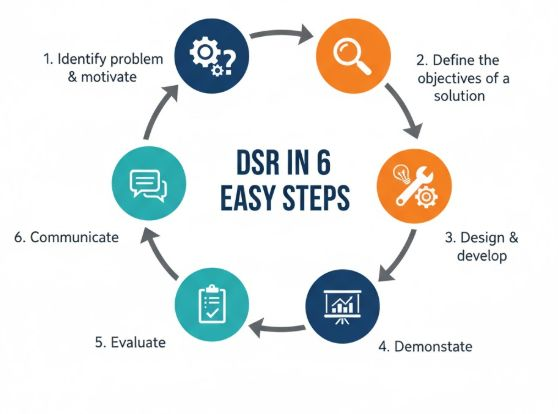
\includegraphics[width=0.75\textwidth]{img/DSR.png}
	\caption[Etapas de la metodología \emph{Design Science Research}]{Las seis etapas de la metodología \emph{Design Science Research}. Adaptado de: \parencite{peffers_2007_dsrm}}
	\label{fig:dsr-etapas}
\end{figure}

Aunque las etapas se presentan en orden, el proceso no es lineal. Las etapas 3, 4 y 5 forman un ciclo que se ha recorrido varias veces: cada prueba en pista o en el banco de trabajo ha revelado aspectos que mejorar, desde el ajuste de las protecciones del motor hasta la respuesta de los pedales o la usabilidad de la aplicación, y esas conclusiones han vuelto a la etapa de diseño. Cada vuelta completa a este ciclo se ha cerrado con una nueva versión del sistema, lo que enlaza la metodología de investigación con la de gestión que se describe a continuación.

%======================================================================
\section{Metodología Kanban}
\label{sec:metodologia-gestion}

Kanban se basa en hacer visible el trabajo. Cada tarea se representa como una tarjeta en un tablero dividido en columnas, una por cada estado por el que pasa, de modo que se ve de un vistazo qué está pendiente, qué está en marcha y qué se ha terminado. Además, se limita el número de tareas que pueden estar en curso a la vez (límite WIP, del inglés \emph{work in progress}). Una tarea nueva solo empieza cuando otra termina, lo que obliga a acabar lo empezado antes de abrir nuevos frentes. El objetivo es que las tareas avancen por el tablero de forma continua. Si se acumulan en una columna, señalan un cuello de botella que hay que resolver. A diferencia de otras metodologías ágiles, Kanban no divide el trabajo en iteraciones de duración fija ni impone roles o reuniones. Las tareas se incorporan al tablero en cuanto aparecen y se atienden por orden de prioridad, y el proceso se ajusta poco a poco según lo que muestra el propio tablero.

El tablero del proyecto tiene cuatro columnas. En \emph{Pendiente} están las tareas identificadas, ordenadas por prioridad. En \emph{En curso}, las que se están desarrollando, con un máximo de tres a la vez. En \emph{En pruebas}, las terminadas que deben validarse sobre el hardware real o en un simulador. En \emph{Hecho}, las ya validadas e integradas en el sistema. Cada tarea se etiqueta además según el subsistema al que pertenece (volante, pedalera, aro o aplicación) y según su tipo (nueva funcionalidad, corrección o documentación).

Para dar estructura al flujo continuo, las tareas se agrupan en versiones. Cada versión se cierra cuando todas sus tareas han pasado por la columna de pruebas. Se numera siguiendo el versionado semántico \parencite{semver_web} (v\emph{X}.\emph{Y}.\emph{Z}): el primer número cambia con las modificaciones incompatibles, el segundo con las funcionalidades nuevas y el tercero con las correcciones. Cada versión publicada coincide con una vuelta completa al ciclo de diseño y evaluación de la DSR.

%======================================================================
\section{Herramientas}
\label{sec:herramientas}

Para aplicar la metodología de gestión se ha utilizado \textbf{GitHub} \parencite{github_docs}, la plataforma en la que se aloja el repositorio oficial del proyecto. Reunir en un mismo sitio el tablero de tareas, el código y las publicaciones evita mantener herramientas separadas y permite enlazar directamente cada tarea con su resultado. En concreto, se han empleado las siguientes funciones:

\begin{itemize}
	\item \textbf{GitHub Projects}: proporciona el tablero Kanban con las cuatro columnas descritas en la sección~\ref{sec:metodologia-gestion}. Las tarjetas se mueven de una columna a otra a medida que avanza el trabajo, y el tablero se filtra por etiquetas para ver solo un subsistema.
	\item \textbf{GitHub Issues}: cada tarea del tablero es una incidencia (\emph{issue}) con su descripción, sus etiquetas y su historial de comentarios. Las incidencias también son el canal por el que los usuarios notifican fallos, según se indica en el apartado de soporte del repositorio, de modo que los problemas detectados por terceros entran directamente en la columna de pendientes.
	\item \textbf{Milestones}: cada versión planificada se representa como un hito al que se asignan sus incidencias. El porcentaje de incidencias cerradas indica el avance de la versión.
	\item \textbf{GitHub Releases}: cuando una versión se completa, se publica con su instalador de Windows y los firmwares de los tres periféricos. Esta función materializa la etapa de comunicación de la DSR y sirve como registro histórico de la evolución del sistema.
	\item \textbf{Git}: el control de versiones del código fuente. Cada cambio queda registrado y puede asociarse a la incidencia que resuelve, lo que permite rastrear qué modificación corresponde a cada tarea.
\end{itemize}

\begin{figure}[htbp]
	\centering
	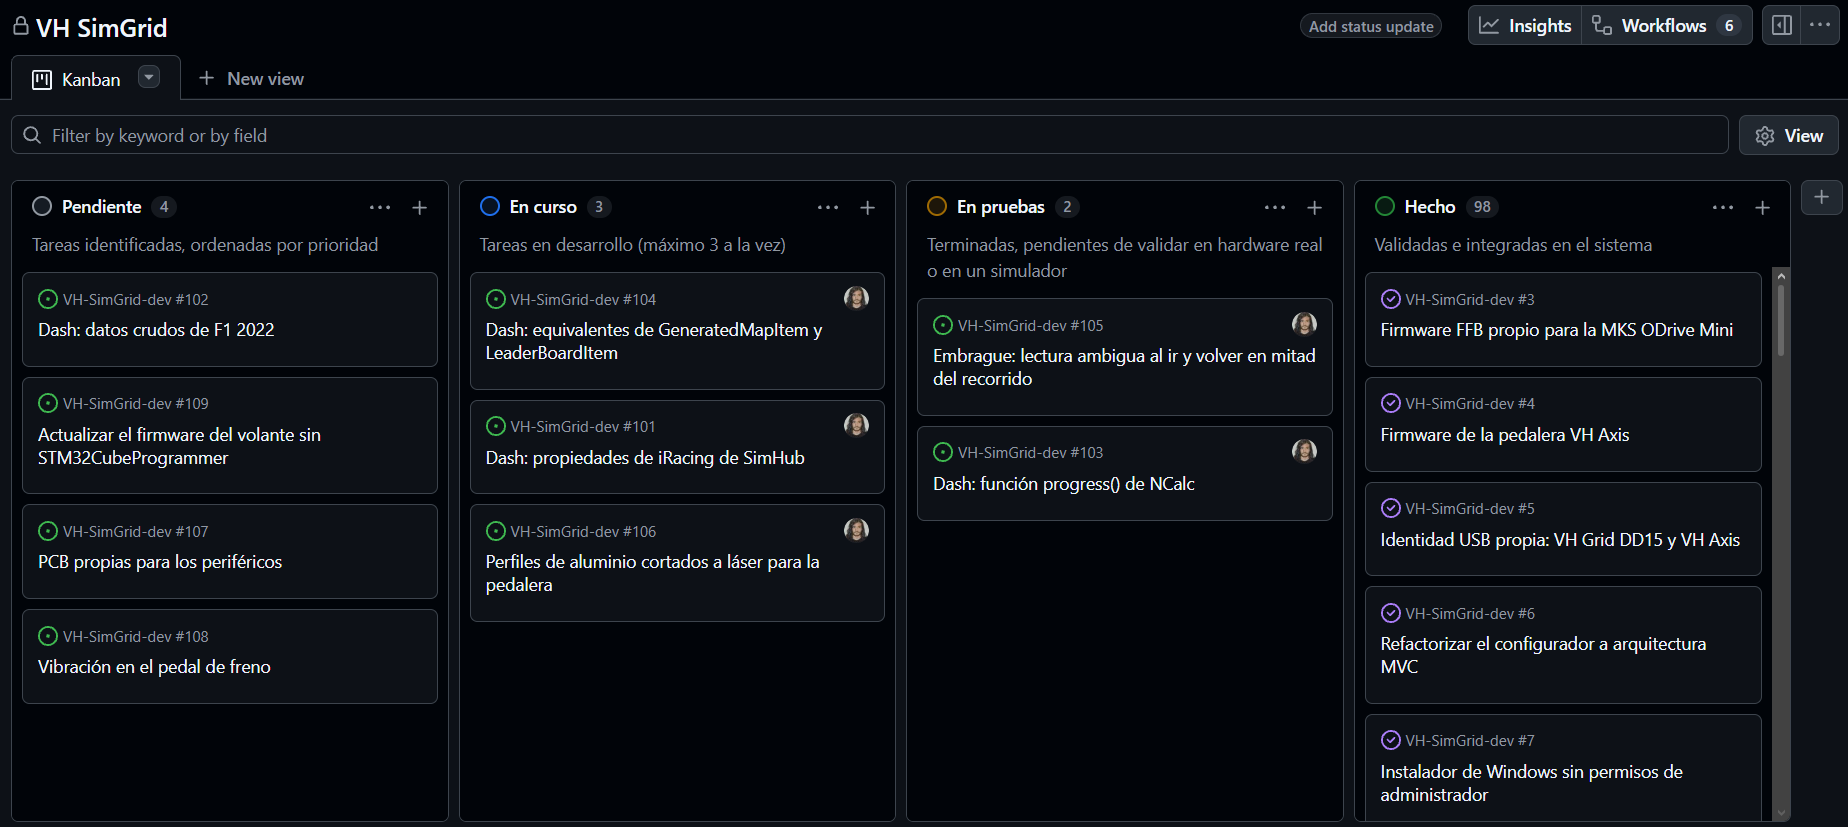
\includegraphics[width=\textwidth]{img/Kanban.png}
	\caption[Tablero Kanban del proyecto en GitHub Projects]{Tablero Kanban del proyecto en GitHub Projects, con las columnas Pendiente, En curso, En pruebas y Hecho. (Fuente propia)}
	\label{fig:kanban}
\end{figure}

En conjunto, estas herramientas cubren todo el recorrido de una tarea: su aparición como incidencia, su planificación en un hito, su seguimiento en el tablero, su implementación en el código y su entrega final en una versión publicada.
	% !TeX root = ../main.tex
\chapter{Planificación}
\label{cap:planificacion}

Para conseguir un correcto desarrollo del proyecto es necesario establecer una planificación detallada que organice las distintas fases del trabajo a lo largo del curso.

El TFG de Ingeniería Multimedia en la Universidad de Alicante corresponde a 12 créditos ECTS, es decir, 300 horas de trabajo. El proyecto se plantea desde septiembre de 2026 con la defensa como horizonte en mayo de 2027, lo que deja nueve meses para repartir la carga de forma progresiva. Además, debe compaginarse con el resto de asignaturas del curso, las prácticas y otros trabajos puntuales, por lo que la planificación se ha diseñado con cierto margen para absorber estas cargas adicionales sin comprometer los plazos de
entrega.

La naturaleza del proyecto condiciona el reparto de horas. VH SimGrid no es solo una aplicación de escritorio: incluye tres periféricos físicos (el volante de \textit{force feedback} VH Grid DD15, la pedalera VH Axis y el aro VH Formula Apex), cada uno con su propio firmware, y una aplicación que los configura en vivo y añade dash, ingeniero de pista por voz y análisis de telemetría. Por ello, la fase de implementación y evaluación concentra la mayor parte del esfuerzo, y las pruebas se realizan sobre el hardware real y con
simuladores comerciales.

Siguiendo la metodología DSR descrita en el capítulo anterior, la planificación temporal se organiza en torno a sus fases principales, complementadas con el uso de un tablero Kanban para la gestión diaria del trabajo.

\begin{table}[H]
	\centering
	\renewcommand{\arraystretch}{2}
	\begin{tabular}{|l|p{4cm}|l|}
		\hline
		\textbf{Fase} & \textbf{Duración estimada} & \textbf{Fecha límite} \\
		\hline
		Identificación del problema y objetivos & 40 horas & 31/10/2026 \\
		\hline
		Diseño y desarrollo de la solución & 55 horas & 31/12/2026 \\
		\hline
		Implementación y evaluación & 140 horas & 15/04/2027 \\
		\hline
		Comunicación & 65 horas & 31/05/2027 \\
		\hline
		\textbf{Total} & \textbf{300 horas} & \\
		\hline
	\end{tabular}
	\caption{Planificación temporal resumida del TFG}
	\label{tab:planificacion}
\end{table}

A continuación se describe el contenido de cada fase:

\begin{itemize}
	\item \textbf{Identificación del problema y objetivos (40 h).} Planificación
	del trabajo, introducción y propuesta de solución, definición de objetivos, elección de la metodología y estudio del estado del arte: periféricos comerciales de simracing, proyectos DIY de \textit{force feedback} y software de configuración, dashes y telemetría existente.
	
	\item \textbf{Diseño y desarrollo de la solución (55 h).} Análisis y especificación de requisitos de los periféricos y de la aplicación, y diseño del sistema: arquitectura hardware (controladora del motor, electrónica de la pedalera y del aro), protocolo de comunicación entre firmware y aplicación, arquitectura de la aplicación y diseño de su interfaz.
	
	\item \textbf{Implementación y evaluación (140 h).} Desarrollo de los tres firmwares (FFB nativo por USB HID PID en el volante, lectura de sensores Hall y célula de carga en la pedalera, LEDs, botones y encoders en el aro), de la aplicación de configuración en vivo, de las funciones de telemetría (dash, ingeniero de pista y análisis) y su documentación. Se cierra con las pruebas
	y la validación sobre hardware real y en los simuladores compatibles, incluida la evaluación de las protecciones de seguridad del volante.
	
	\item \textbf{Comunicación (65 h).} Redacción final de la memoria
	(resumen, motivación, resultados, conclusiones y trabajo futuro), revisión de bibliografía y glosario, y preparación de la defensa del TFG en mayo de 2027.
\end{itemize}

Para complementar esta visión, en la sección~\ref{sec:gantt} se presenta un diagrama de Gantt que muestra de forma gráfica las fases del proyecto y sus duraciones, detallando las tareas en las que se ha dividido cada una de ellas.

% ---------- Página en horizontal para el Gantt ----------
\newpage
\begin{landscape}
	\thispagestyle{empty}
	\section{Diagrama de Gantt}
	\label{sec:gantt}
	\begin{figure}[H]
		\centering
		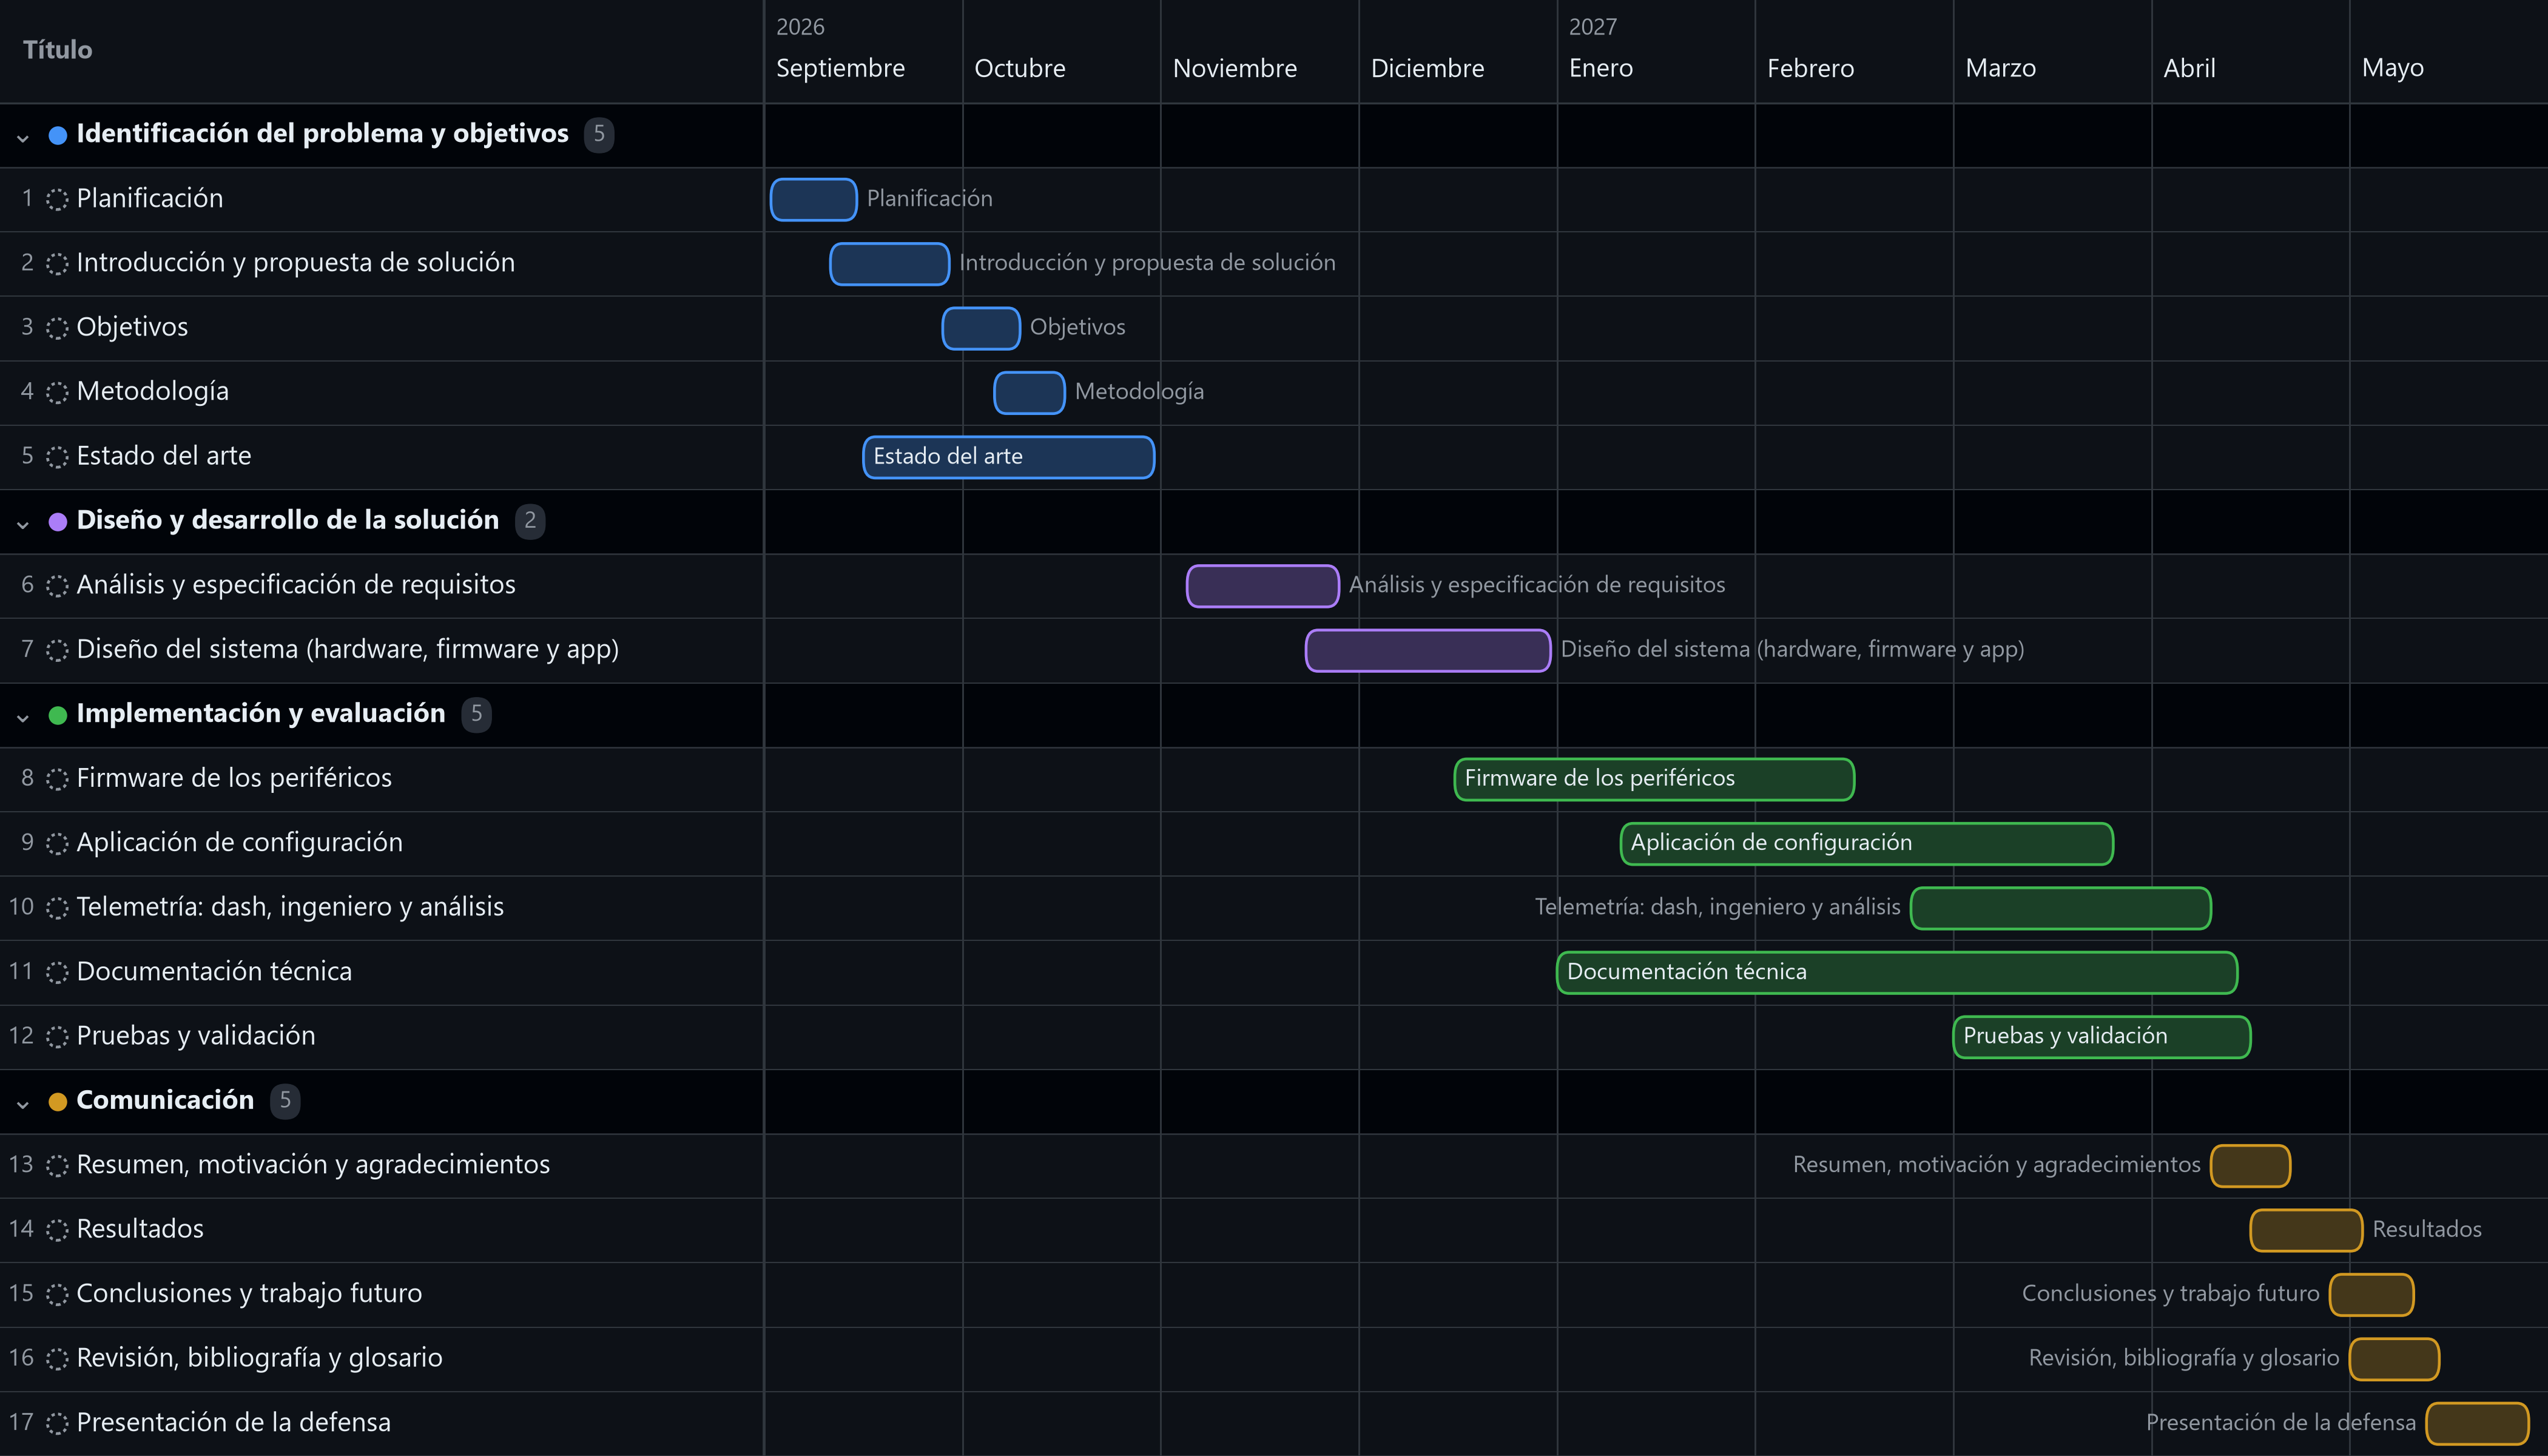
\includegraphics[width=\linewidth, height=0.8\textheight, keepaspectratio]{img/gantt_github.png}
		\caption[Diagrama de Gantt]{Diagrama de Gantt. (Fuente propia)}
		\label{fig:gantt}
	\end{figure}
\end{landscape}
	% !TeX root = ../main.tex
\chapter{Análisis y especificación de requisitos}
\label{cap:requisitos}
En el capítulo~\ref{cap:objetivos} se fijaron los objetivos del trabajo, es decir, qué se pretende conseguir con el sistema planteado, VH SimGrid. Este capítulo traduce esos objetivos en requisitos, es decir, en enunciados concretos y verificables de lo que el sistema debe hacer y de las condiciones en que debe hacerlo. Los requisitos son el punto de partida del diseño y de la implementación, que se describen en los capítulos siguientes, y la referencia frente a la que se valida el resultado.

La especificación sigue la práctica IEEE~830-1998 para la especificación de requisitos del software (\emph{Software Requirements Specification}, SRS)~\cite{ieee830}, que es la referencia clásica en ingeniería del software. Esta norma fue sustituida por la ISO/IEC/IEEE~29148~\cite{iso29148}, que recoge su contenido y lo amplía a los requisitos de sistema (\emph{System Requirements Specification}, SyRS), es decir, a productos que combinan hardware y software. Como VH SimGrid es precisamente un sistema de este tipo, formado por tres periféricos con su firmware y una aplicación de escritorio, se adopta la estructura de capítulos de la IEEE~830 y se completa con lo que la ISO/IEC/IEEE~29148 añade para los sistemas, las interfaces hardware, las restricciones físicas y de fabricación y la trazabilidad de cada requisito hasta los objetivos de los que procede.

La IEEE~830 enumera las características que debe reunir una buena especificación, y que se han tenido en cuenta al redactar los requisitos: deben ser \textbf{correctos}, porque cada uno responde a una necesidad real del sistema; \textbf{inequívocos}, con una única interpretación posible; \textbf{completos}, cubriendo todas las funciones y restricciones relevantes; \textbf{consistentes}, sin contradicciones entre ellos; \textbf{clasificados} por prioridad; \textbf{verificables}, con un procedimiento finito que permita comprobar su cumplimiento; \textbf{modificables}, gracias a una estructura y una numeración ordenadas; y \textbf{trazables}, de modo que se conozca el origen de cada requisito y se pueda seguir en las fases posteriores.

\section{Descripción general}
\label{sec:req-descripcion}
\subsection{Perspectiva del producto}
\label{subsec:perspectiva}
VH SimGrid nace como un ecosistema independiente: no es la evolución de ningún sistema anterior ni un componente de un sistema mayor. Está formado por cuatro subsistemas, que coinciden con los grupos de objetivos funcionales del capítulo~\ref{cap:objetivos}:

\begin{itemize}
	\item \textbf{VH Grid DD15}: base de volante \emph{direct drive} con force feedback, construida sobre una controladora MKS ODrive Mini (STM32F405) y un motor de patinete eléctrico.
	\item \textbf{VH Axis}: pedalera de tres pedales, con sensores Hall en el acelerador y el embrague y una célula de carga en el freno, gobernada por un Arduino Micro.
	\item \textbf{VH Formula Apex}: aro con tira de LEDs, matriz de botones, encoders, palancas de embrague y una pantalla, gobernado por un ATmega32U4.
	\item \textbf{Aplicación VH SimGrid}: aplicación de escritorio para Windows que configura los tres periféricos en vivo y reúne el dash, el ingeniero de pista y el análisis de telemetría.
\end{itemize}

Aunque el producto es autónomo, se integra en un entorno que no controla: desde el sistema operativo Windows y la interfaz DirectInput, a través de la cual los simuladores leen los mandos y envían el force feedback, hasta los propios simuladores, que publican la telemetría de la sesión. La figura~\ref{fig:contexto} muestra este contexto. Los periféricos tienen dos vías de comunicación con el PC: la misma que usa cualquier mando USB, por la que el simulador lee los ejes y los botones y envía los efectos de fuerza, y una vía de configuración por la que la aplicación ajusta sus parámetros. Esta separación permite que los periféricos funcionen como mandos normales aunque la aplicación esté cerrada.
 
% Diagrama de contexto: subsistemas propios (gris) y elementos externos (borde discontinuo).
% Abajo, los tres periféricos; arriba, la aplicación, Windows, el simulador y la pantalla del dash.
\begin{figure}[H]
	\centering
	\resizebox{\textwidth}{!}{%
		\begin{tikzpicture}[
			>=Stealth,
			caja/.style={draw, thick, rounded corners, align=center, minimum width=3.3cm, minimum height=1.1cm, font=\small},
			externo/.style={caja, dashed, fill=gray!8},
			propio/.style={caja, fill=gray!22},
			etiq/.style={font=\scriptsize, align=center, fill=white, inner sep=1pt}
			]
			\node[externo] (pantalla) at (-7,2) {Monitor del dash\\o dispositivo móvil};
			\node[propio]  (app)      at (-3,0) {Aplicación\\VH SimGrid};
			\node[externo] (os)       at (3,0)  {Windows\\(DirectInput, USB HID)};
			\node[externo] (sim)      at (7,2)  {Simulador de\\conducción};
			\node[propio]  (dd)       at (-5,-3.6) {Volante\\VH Grid DD15};
			\node[propio]  (axis)     at (0,-3.6)  {Pedalera\\VH Axis};
			\node[propio]  (apex)     at (5,-3.6)  {Aro\\VH Formula Apex};

			\draw[->, thick] (sim.west) -- node[etiq, above] {telemetría (memoria compartida o UDP)} (sim.west -| app.north) -- (app.north);
			\draw[<->, thick] (sim.south) |- node[etiq, pos=0.25, right] {ejes, botones\\y efectos FFB} (os.east);
			\draw[->, thick] (app.west) -| node[etiq, pos=0.3, above] {dash} (pantalla.south);
			\foreach \p in {dd, axis, apex} {
				\draw[<->, thick] (os.south) -- (\p.north);
				\draw[<->, thick, dashed] (app.south) -- (\p.north);
			}
			\node[etiq] at (2.2,-1.6) {USB HID};
			\node[etiq] at (-2.6,-1.6) {configuración};
	\end{tikzpicture}}
	\caption[Diagrama de contexto de VH SimGrid]{Diagrama de contexto de VH SimGrid. En gris oscuro, los subsistemas propios; con borde discontinuo, los elementos externos. (Fuente propia)}
	\label{fig:contexto}
\end{figure}

 
 Siguiendo la IEEE~830, la perspectiva del producto se completa con la descripción de sus interfaces y sus condiciones de operación:
 
 \begin{description}
 	\item[Interfaces de usuario.] El piloto interactúa con el sistema de tres formas. La primera es la aplicación de escritorio, organizada en páginas (Inicio, Volante, Aro, Pedalera, Dash, Ingeniero, Análisis y Ajustes), desde la que calibra y personaliza los periféricos, configura el ingeniero de pista virtual y analiza sus sesiones en detalle con todos los parámetros de telemetría registrados. La segunda son los mandos y la pantalla del aro, con los que consulta el dash y cambia ajustes durante la conducción. La tercera es la voz: el ingeniero le informa por radio mientras está en pista y responde a sus preguntas.
 	\item[Interfaces hardware.] Los tres periféricos se conectan al PC por USB. La base force feedback necesita además una fuente de alimentación para el motor, dimensionada para la corriente de pico de la controladora. El ingeniero requiere un micrófono y unos altavoces o auriculares, y el dash, un monitor adicional o un dispositivo móvil.
 	\item[Interfaces software.] El volante se presenta a Windows como un dispositivo USB HID con el perfil de force feedback PID (\emph{Physical Interface Device}), que DirectInput reconoce de forma nativa. La pedalera y el aro se presentan como mandos HID estándar. La aplicación lee la telemetría de los simuladores por los medios que cada uno ofrece: memoria compartida en la mayoría de los simuladores de circuito y paquetes UDP en otros, como la saga F1 o los títulos de rally.
 	\item[Interfaces de comunicaciones.] Toda la comunicación con los periféricos es local, por USB. El dash en un móvil usa la red local, y el móvil se vincula escaneando un código QR. El sistema no necesita conexión a Internet salvo para comprobar si hay versiones nuevas.
 	\item[Restricciones de memoria.] El firmware debe caber en los microcontroladores elegidos: 1~MB de flash y 192~kB de RAM en el STM32F405 del volante, y 32~kB de flash y 2,5~kB de RAM en los ATmega32U4 de la pedalera y del aro. La configuración persistente se guarda en la flash del volante y en la EEPROM de los otros dos periféricos.
 	\item[Operaciones.] El uso normal no requiere intervención técnica: los periféricos se detectan solos y los ajustes se aplican en vivo. Las únicas operaciones de mantenimiento son la actualización del firmware, que se hace desde la aplicación, y el primer flasheo de la base force feedback, que se hace una sola vez con STM32CubeProgrammer.
 \end{description}
 
 En cuanto a las \textbf{funciones del producto}, el sistema permite al piloto conducir con force feedback, pedales y mandos propios en cualquier simulador compatible con DirectInput; ajustar cada periférico en vivo y guardar esos ajustes en perfiles; recibir información de la carrera en las luces del aro, en un dash y por la voz del ingeniero; planificar la estrategia de carrera; y analizar después las sesiones grabadas. La sección~\ref{sec:req-especificos} detalla cada una de estas funciones.
 
 
\subsection{Características de los actores}
\label{subsec:actores}

Los usuarios de VH SimGrid se agrupan en los perfiles de la tabla~\ref{tab:actores}. Se distinguen por su relación con el sistema y por sus conocimientos técnicos, que condicionan los requisitos de usabilidad. A ellos se suma un actor que no es una persona, el simulador de conducción, que participa en los casos de uso como fuente de la telemetría y destino de los mandos.

\begin{table}[H]
	\centering
	\renewcommand{\arraystretch}{1.5}
	\small
	\begin{tabularx}{\textwidth}{|>{\raggedright\arraybackslash}p{2.6cm}|>{\raggedright\arraybackslash}X|>{\raggedright\arraybackslash}p{3.9cm}|}
		\hline
		\textbf{Actor} & \textbf{Descripción} & \textbf{Conocimientos} \\
		\hline
		Piloto aficionado & Usuario principal. Corre en simuladores de forma habitual y quiere un equipo que funcione al conectarlo, con ajustes sencillos y perfiles ya preparados. & Uso general de Windows y de los simuladores. Ninguno de electrónica ni de programación. \\
		\hline
		Piloto avanzado & Busca exprimir el equipo: afina el force feedback por bandas, diseña sus dashes, planifica estrategias y analiza su telemetría vuelta a vuelta. & Conoce los conceptos de reglaje y de telemetría. No necesita conocimientos de electrónica. \\
		\hline
		Constructor & Monta los periféricos a partir de los componentes, graba el primer firmware del volante y resuelve las incidencias de hardware. & Electrónica básica, soldadura y montaje mecánico. Uso de herramientas de flasheo. \\
		\hline
		Simulador de conducción & Actor externo, no humano. Publica la telemetría de la sesión y se comunica con los periféricos a través de DirectInput. & No aplica. \\
		\hline
	\end{tabularx}
	\caption{Perfiles de los actores del sistema}
	\label{tab:actores}
\end{table}

En la práctica una misma persona puede desempeñar varios perfiles. Separar en actores permite, sin embargo, diseñar cada parte del sistema para quien de verdad la va a usar: la aplicación se piensa para un piloto aficionado, mientras que las tareas que requieren conocimientos técnicos quedan limitadas al montaje y al primer flasheo.

\subsection{Restricciones generales}
\label{subsec:restricciones}
El desarrollo está sujeto a varias restricciones que no surgen de lo que el sistema debe hacer, sino del contexto en el que se construye. Limitan las decisiones de diseño y se reflejan en varios requisitos no funcionales.

\begin{description}
	\item[Presupuesto.] Por coherencia con el objetivo ONF-11, el coste total de los materiales del equipo debe quedar claramente por debajo del de un puesto comercial de gama media de prestaciones equivalentes, que, como se vio en el capítulo~\ref{cap:problema-solucion}, supera los 1.200~€.
	\item[Componentes disponibles.] Solo se emplean componentes que se pueden comprar al por menor en tiendas de electrónica o en línea, sin pedidos mínimos industriales ni piezas a medida. De ahí la elección de una controladora de motor de código abierto (MKS ODrive Mini, compatible con ODrive), un motor de buje de patinete eléctrico como motor de par, placas Arduino y microcontroladores ATmega32U4, sensores Hall, una célula de carga con un amplificador INA333, LEDs WS2812 y un expansor de E/S MCP23017. El firmware debe adaptarse a lo que estos componentes ofrecen, y no al revés.
	\item[Fabricación casera.] Todas las piezas deben poder fabricarse y montarse con herramientas de taller doméstico, sin maquinaria industrial. Esto condiciona la mecánica de los periféricos y obliga a que el software compense algunas limitaciones del hardware, como el rizado magnético (\emph{cogging}) del motor de patinete, que se corrige con una calibración en el firmware.
	\item[Plataforma.] La aplicación se desarrolla solo para Windows 10 y 11, que es el sistema en el que se ejecutan prácticamente todos los simuladores de conducción.
	\item[Licencias.] Los componentes de terceros (el núcleo del firmware ODrive, TinyUSB, el descriptor HID PID derivado de OpenFFBoard, Piper, Vosk y las voces del ingeniero) imponen sus propias licencias, cuyos avisos y atribuciones deben respetarse en la distribución.
	\item[Recursos humanos y tiempo.] El sistema lo desarrolla una sola persona, en el plazo fijado en la planificación (capítulo~\ref{cap:planificacion}). Esto obliga a priorizar los requisitos y a reutilizar componentes probados cuando existen.
\end{description}

\subsection{Suposiciones y dependencias}
\label{subsec:suposiciones}
Los requisitos se han redactado dando por ciertas las siguientes condiciones. Si alguna dejara de cumplirse, los requisitos afectados tendrían que revisarse.

\begin{enumerate}
	\item El PC del usuario ejecuta Windows 10 u 11 y tiene puertos USB libres para los tres periféricos.
	\item Los simuladores siguen admitiendo volantes con force feedback a través de DirectInput y del perfil HID PID, como hacen hoy los títulos compatibles.
	\item Los simuladores siguen publicando su telemetría por memoria compartida o por UDP, y el usuario activa en cada juego la opción de telemetría cuando es necesaria. El formato de estos datos lo define cada desarrollador y puede cambiar entre versiones.
	\item La base dispone de una fuente de alimentación capaz de entregar la corriente que pide el motor, y el montaje mecánico fija la base con firmeza.
	\item El equipo tiene potencia suficiente para ejecutar en local la síntesis de voz (Piper) y el reconocimiento de voz (Vosk) mientras corre el simulador.
	\item La controladora del volante llega de fábrica sin el firmware propio, por lo que su primer flasheo debe hacerse por DFU con el puente BOOT0. A partir de entonces, todas las actualizaciones se hacen desde la aplicación.
\end{enumerate}

\section{Requisitos específicos}
\label{sec:req-especificos}

Esta sección especifica los requisitos de VH SimGrid con el nivel de detalle necesario para diseñar el sistema y comprobar después que los cumple. Siguiendo la IEEE~830~\cite{ieee830}, se distinguen dos tipos: los requisitos funcionales, que describen lo que el sistema debe hacer (apartado~\ref{subsec:rf}), y los requisitos no funcionales, que fijan las cualidades con que debe hacerlo, como la latencia, la seguridad o el coste (apartado~\ref{subsec:rnf}).

Cada requisito se describe en una tabla con los siguientes campos:

\begin{description}
	\item[Identificador.] Código único formado por el prefijo \textbf{RF} (requisito funcional) o \textbf{RNF} (requisito no funcional) y un número correlativo. Permite referirse al requisito sin ambigüedad en el resto de la memoria.
	\item[Nombre.] Título breve que resume el requisito.
	\item[Prioridad.] Importancia del requisito para el producto, según la clasificación que propone la IEEE~830: \textbf{Alta}, si el sistema no es aceptable sin él (esencial); \textbf{Media}, si aporta un valor importante pero su ausencia no impide usar el sistema (condicional); y \textbf{Baja}, si es una mejora que puede posponerse (opcional).
	\item[Actores.] Solo en los requisitos funcionales: los actores de la tabla~\ref{tab:actores} que intervienen en la función.
	\item[Descripción.] Enunciado del requisito. Se redacta de forma inequívoca y, siempre que es posible, con un valor medible, para que su cumplimiento pueda verificarse.
\end{description}

Al final de la sección, la matriz de trazabilidad relaciona cada requisito con el objetivo específico del capítulo~\ref{cap:objetivos} del que procede.

\subsection{Requisitos funcionales}
\label{subsec:rf}

Los requisitos funcionales describen los servicios que el sistema debe proporcionar y su comportamiento ante cada entrada. Se agrupan por subsistema, siguiendo la misma división que la perspectiva del producto (apartado~\ref{subsec:perspectiva}): la base \emph{direct drive}, la pedalera, el aro y su pantalla, y la aplicación. Esta última, por su amplitud, se divide a su vez en gestión de los periféricos, telemetría y dash, ingeniero de pista y análisis de telemetría.

\subsubsection{Base \emph{direct drive} VH Grid DD15}

La base es el periférico más exigente del sistema: debe ser reconocida como un volante con force feedback y transmitir al piloto las fuerzas que calcula el simulador. Sus requisitos funcionales se recogen en las tablas~\ref{tab:rf1} a~\ref{tab:rf10}.

\begin{table}[H]
	\centering
	\renewcommand{\arraystretch}{2}
	\begin{tabular}{|l|p{10cm}|}
		\hline
		Identificador & RF1 \\
		\hline
		Nombre & Volante FFB nativo \\
		\hline
		Prioridad & Alta \\
		\hline
		Actores & Piloto, simulador \\
		\hline
		Descripción & La base se presentará a Windows como un volante USB HID con force feedback PID, sin instalar drivers ni dejar programas residentes. \\
		\hline
	\end{tabular}
	\caption{Requisito funcional RF1 (Volante FFB nativo)}
	\label{tab:rf1}
\end{table}

\begin{table}[H]
	\centering
	\renewcommand{\arraystretch}{2}
	\begin{tabular}{|l|p{10cm}|}
		\hline
		Identificador & RF2 \\
		\hline
		Nombre & Efectos DirectInput \\
		\hline
		Prioridad & Alta \\
		\hline
		Actores & Piloto, simulador \\
		\hline
		Descripción & La base reproducirá los efectos de fuerza constante, muelle, amortiguación, fricción e inercia que envíe el simulador, cada uno con su ganancia ajustable. \\
		\hline
	\end{tabular}
	\caption{Requisito funcional RF2 (Efectos DirectInput)}
	\label{tab:rf2}
\end{table}

\begin{table}[H]
	\centering
	\renewcommand{\arraystretch}{2}
	\begin{tabular}{|l|p{10cm}|}
		\hline
		Identificador & RF3 \\
		\hline
		Nombre & Rango de giro y centrado \\
		\hline
		Prioridad & Alta \\
		\hline
		Actores & Piloto \\
		\hline
		Descripción & El usuario podrá ajustar el rango de giro entre 90$^{\circ}$ y 1440$^{\circ}$ y fijar el centro del volante. \\
		\hline
	\end{tabular}
	\caption{Requisito funcional RF3 (Rango de giro y centrado)}
	\label{tab:rf3}
\end{table}

\begin{table}[H]
	\centering
	\renewcommand{\arraystretch}{2}
	\begin{tabular}{|l|p{10cm}|}
		\hline
		Identificador & RF4 \\
		\hline
		Nombre & Sensación general \\
		\hline
		Prioridad & Alta \\
		\hline
		Actores & Piloto \\
		\hline
		Descripción & El usuario podrá ajustar la fuerza máxima, el suavizado de la señal, el refuerzo de las fuerzas pequeñas y la dureza del tope de giro. \\
		\hline
	\end{tabular}
	\caption{Requisito funcional RF4 (Sensación general)}
	\label{tab:rf4}
\end{table}

\begin{table}[H]
	\centering
	\renewcommand{\arraystretch}{2}
	\begin{tabular}{|l|p{10cm}|}
		\hline
		Identificador & RF5 \\
		\hline
		Nombre & Efectos base \\
		\hline
		Prioridad & Media \\
		\hline
		Actores & Piloto \\
		\hline
		Descripción & La base aplicará una amortiguación, una fricción y una inercia propias, independientes del juego y ajustables por el usuario. \\
		\hline
	\end{tabular}
	\caption{Requisito funcional RF5 (Efectos base)}
	\label{tab:rf5}
\end{table}

\begin{table}[H]
	\centering
	\renewcommand{\arraystretch}{2}
	\begin{tabular}{|l|p{10cm}|}
		\hline
		Identificador & RF6 \\
		\hline
		Nombre & Ecualizador FFB \\
		\hline
		Prioridad & Media \\
		\hline
		Actores & Piloto \\
		\hline
		Descripción & La base filtrará la señal de fuerza con un ecualizador de 6 bandas entre 5 y 60~Hz, con una ganancia de 0 a 500~\% por banda. \\
		\hline
	\end{tabular}
	\caption{Requisito funcional RF6 (Ecualizador FFB)}
	\label{tab:rf6}
\end{table}

\begin{table}[H]
	\centering
	\renewcommand{\arraystretch}{2}
	\begin{tabular}{|l|p{10cm}|}
		\hline
		Identificador & RF7 \\
		\hline
		Nombre & Curva FFB \\
		\hline
		Prioridad & Media \\
		\hline
		Actores & Piloto \\
		\hline
		Descripción & La base aplicará una curva de respuesta de 9 puntos entre la fuerza pedida por el juego y la entregada por el motor, con preajustes. \\
		\hline
	\end{tabular}
	\caption{Requisito funcional RF7 (Curva FFB)}
	\label{tab:rf7}
\end{table}

\begin{table}[H]
	\centering
	\renewcommand{\arraystretch}{2}
	\begin{tabular}{|l|p{10cm}|}
		\hline
		Identificador & RF8 \\
		\hline
		Nombre & Calibración anti-cogging \\
		\hline
		Prioridad & Media \\
		\hline
		Actores & Piloto, constructor \\
		\hline
		Descripción & La base medirá el rizado magnético del motor, lo compensará y guardará la calibración en su memoria flash. \\
		\hline
	\end{tabular}
	\caption{Requisito funcional RF8 (Calibración anti-cogging)}
	\label{tab:rf8}
\end{table}

\begin{table}[H]
	\centering
	\renewcommand{\arraystretch}{2}
	\begin{tabular}{|l|p{10cm}|}
		\hline
		Identificador & RF9 \\
		\hline
		Nombre & Monitorización \\
		\hline
		Prioridad & Media \\
		\hline
		Actores & Piloto \\
		\hline
		Descripción & La aplicación mostrará el estado del motor en vivo y un registro de los últimos segundos del giro y de la fuerza, con la línea de saturación marcada. \\
		\hline
	\end{tabular}
	\caption{Requisito funcional RF9 (Monitorización)}
	\label{tab:rf9}
\end{table}

\begin{table}[H]
	\centering
	\renewcommand{\arraystretch}{2}
	\begin{tabular}{|l|p{10cm}|}
		\hline
		Identificador & RF10 \\
		\hline
		Nombre & Reinicio y mantenimiento \\
		\hline
		Prioridad & Baja \\
		\hline
		Actores & Piloto, constructor \\
		\hline
		Descripción & El usuario podrá reiniciar la base y consultar sus opciones de mantenimiento desde la aplicación. \\
		\hline
	\end{tabular}
	\caption{Requisito funcional RF10 (Reinicio y mantenimiento)}
	\label{tab:rf10}
\end{table}

\subsubsection{Pedalera VH Axis}

La pedalera debe medir la posición del acelerador y del embrague y la fuerza aplicada sobre el freno, y permitir calibrarlos y ajustar su respuesta (tablas~\ref{tab:rf11} a~\ref{tab:rf15}).

\begin{table}[H]
	\centering
	\renewcommand{\arraystretch}{2}
	\begin{tabular}{|l|p{10cm}|}
		\hline
		Identificador & RF11 \\
		\hline
		Nombre & Tres ejes \\
		\hline
		Prioridad & Alta \\
		\hline
		Actores & Piloto, simulador \\
		\hline
		Descripción & La pedalera se presentará como un mando USB con tres ejes: acelerador y embrague, medidos por posición con sensores Hall, y freno, medido por fuerza con una célula de carga. \\
		\hline
	\end{tabular}
	\caption{Requisito funcional RF11 (Tres ejes)}
	\label{tab:rf11}
\end{table}

\begin{table}[H]
	\centering
	\renewcommand{\arraystretch}{2}
	\begin{tabular}{|l|p{10cm}|}
		\hline
		Identificador & RF12 \\
		\hline
		Nombre & Calibración guiada \\
		\hline
		Prioridad & Alta \\
		\hline
		Actores & Piloto \\
		\hline
		Descripción & La aplicación guiará la calibración del reposo y del fondo de cada pedal, y la del freno se expresará en kilos. \\
		\hline
	\end{tabular}
	\caption{Requisito funcional RF12 (Calibración guiada)}
	\label{tab:rf12}
\end{table}

\begin{table}[H]
	\centering
	\renewcommand{\arraystretch}{2}
	\begin{tabular}{|l|p{10cm}|}
		\hline
		Identificador & RF13 \\
		\hline
		Nombre & Curva de respuesta \\
		\hline
		Prioridad & Media \\
		\hline
		Actores & Piloto \\
		\hline
		Descripción & Cada pedal tendrá una curva de respuesta editable arrastrando sus puntos, con preajustes, zona muerta e inversión del sentido. \\
		\hline
	\end{tabular}
	\caption{Requisito funcional RF13 (Curva de respuesta)}
	\label{tab:rf13}
\end{table}

\begin{table}[H]
	\centering
	\renewcommand{\arraystretch}{2}
	\begin{tabular}{|l|p{10cm}|}
		\hline
		Identificador & RF14 \\
		\hline
		Nombre & Guardado automático \\
		\hline
		Prioridad & Alta \\
		\hline
		Actores & Piloto \\
		\hline
		Descripción & Todo cambio de configuración se guardará solo en la EEPROM de la pedalera, sin que el usuario tenga que confirmarlo. \\
		\hline
	\end{tabular}
	\caption{Requisito funcional RF14 (Guardado automático)}
	\label{tab:rf14}
\end{table}

\begin{table}[H]
	\centering
	\renewcommand{\arraystretch}{2}
	\begin{tabular}{|l|p{10cm}|}
		\hline
		Identificador & RF15 \\
		\hline
		Nombre & Traza en vivo \\
		\hline
		Prioridad & Media \\
		\hline
		Actores & Piloto \\
		\hline
		Descripción & La aplicación mostrará la posición de los tres pedales en tiempo real, tanto en su página como en la de inicio. \\
		\hline
	\end{tabular}
	\caption{Requisito funcional RF15 (Traza en vivo)}
	\label{tab:rf15}
\end{table}

\subsubsection{Aro VH Formula Apex}

El aro reúne los mandos que el piloto usa durante la conducción y una tira de LEDs que le informa del régimen del motor y de los eventos de la carrera (tablas~\ref{tab:rf16} a~\ref{tab:rf21}). Su pantalla, por su importancia, se trata en el apartado siguiente.

\begin{table}[H]
	\centering
	\renewcommand{\arraystretch}{2}
	\begin{tabular}{|l|p{10cm}|}
		\hline
		Identificador & RF16 \\
		\hline
		Nombre & Botones y encoders \\
		\hline
		Prioridad & Alta \\
		\hline
		Actores & Piloto, simulador \\
		\hline
		Descripción & El aro leerá su matriz de botones y sus encoders y los enviará al PC como botones de un mando USB estándar. \\
		\hline
	\end{tabular}
	\caption{Requisito funcional RF16 (Botones y encoders)}
	\label{tab:rf16}
\end{table}

\begin{table}[H]
	\centering
	\renewcommand{\arraystretch}{2}
	\begin{tabular}{|l|p{10cm}|}
		\hline
		Identificador & RF17 \\
		\hline
		Nombre & Palancas de embrague \\
		\hline
		Prioridad & Media \\
		\hline
		Actores & Piloto \\
		\hline
		Descripción & El aro leerá las palancas de embrague, con modo de funcionamiento y punto de mordida configurables. \\
		\hline
	\end{tabular}
	\caption{Requisito funcional RF17 (Palancas de embrague)}
	\label{tab:rf17}
\end{table}

\begin{table}[H]
	\centering
	\renewcommand{\arraystretch}{2}
	\begin{tabular}{|l|p{10cm}|}
		\hline
		Identificador & RF18 \\
		\hline
		Nombre & Barra de RPM \\
		\hline
		Prioridad & Alta \\
		\hline
		Actores & Piloto, simulador \\
		\hline
		Descripción & La tira de LEDs mostrará las revoluciones con modo, llenado, reinicio al cambiar de marcha y umbral por LED configurables, y podrá ajustarse sola al régimen de cada coche. \\
		\hline
	\end{tabular}
	\caption{Requisito funcional RF18 (Barra de RPM)}
	\label{tab:rf18}
\end{table}

\begin{table}[H]
	\centering
	\renewcommand{\arraystretch}{2}
	\begin{tabular}{|l|p{10cm}|}
		\hline
		Identificador & RF19 \\
		\hline
		Nombre & Luces por eventos \\
		\hline
		Prioridad & Media \\
		\hline
		Actores & Piloto, simulador \\
		\hline
		Descripción & El usuario podrá asignar a un rango de LEDs eventos de la carrera (banderas, TC, ABS, DRS, ERS, limitador, pit lane, coches cerca, pedales, combustible), con su color y su estilo: fijo, parpadeo, respiración o desplazamiento. \\
		\hline
	\end{tabular}
	\caption{Requisito funcional RF19 (Luces por eventos)}
	\label{tab:rf19}
\end{table}

\begin{table}[H]
	\centering
	\renewcommand{\arraystretch}{2}
	\begin{tabular}{|l|p{10cm}|}
		\hline
		Identificador & RF20 \\
		\hline
		Nombre & Perfiles de luces \\
		\hline
		Prioridad & Baja \\
		\hline
		Actores & Piloto \\
		\hline
		Descripción & Las asignaciones de luces se agruparán en carpetas y se guardarán en perfiles por juego y por coche. \\
		\hline
	\end{tabular}
	\caption{Requisito funcional RF20 (Perfiles de luces)}
	\label{tab:rf20}
\end{table}

\begin{table}[H]
	\centering
	\renewcommand{\arraystretch}{2}
	\begin{tabular}{|l|p{10cm}|}
		\hline
		Identificador & RF21 \\
		\hline
		Nombre & Brillo \\
		\hline
		Prioridad & Media \\
		\hline
		Actores & Piloto \\
		\hline
		Descripción & El usuario podrá ajustar el brillo diurno y nocturno y apagar la tira cuando no haya juego; el aro recordará su brillo aunque arranque sin PC. \\
		\hline
	\end{tabular}
	\caption{Requisito funcional RF21 (Brillo)}
	\label{tab:rf21}
\end{table}

\subsubsection{Pantalla del aro}

La pantalla integrada en el aro muestra el dash al piloto sin que tenga que apartar la vista de la pista y le permite cambiar ajustes del equipo sin soltar el volante (tablas~\ref{tab:rf22} a~\ref{tab:rf28}).

\begin{table}[H]
	\centering
	\renewcommand{\arraystretch}{2}
	\begin{tabular}{|l|p{10cm}|}
		\hline
		Identificador & RF22 \\
		\hline
		Nombre & Pantalla como monitor \\
		\hline
		Prioridad & Alta \\
		\hline
		Actores & Piloto \\
		\hline
		Descripción & La pantalla del aro se conectará al PC como un monitor más, que Windows reconocerá sin drivers adicionales, y la aplicación permitirá elegirla como destino del dash. \\
		\hline
	\end{tabular}
	\caption{Requisito funcional RF22 (Pantalla como monitor)}
	\label{tab:rf22}
\end{table}

\begin{table}[H]
	\centering
	\renewcommand{\arraystretch}{2}
	\begin{tabular}{|l|p{10cm}|}
		\hline
		Identificador & RF23 \\
		\hline
		Nombre & Dashes en la pantalla \\
		\hline
		Prioridad & Alta \\
		\hline
		Actores & Piloto, simulador \\
		\hline
		Descripción & La pantalla del aro mostrará a pantalla completa cualquier dash de la galería o creado en el editor, adaptado a su resolución. \\
		\hline
	\end{tabular}
	\caption{Requisito funcional RF23 (Dashes en la pantalla)}
	\label{tab:rf23}
\end{table}

\begin{table}[H]
	\centering
	\renewcommand{\arraystretch}{2}
	\begin{tabular}{|l|p{10cm}|}
		\hline
		Identificador & RF24 \\
		\hline
		Nombre & Cambio de pantallas del dash \\
		\hline
		Prioridad & Media \\
		\hline
		Actores & Piloto \\
		\hline
		Descripción & El piloto podrá pasar de una pantalla a otra del dash con los botones del aro, sin soltar el volante. \\
		\hline
	\end{tabular}
	\caption{Requisito funcional RF24 (Cambio de pantallas del dash)}
	\label{tab:rf24}
\end{table}

\begin{table}[H]
	\centering
	\renewcommand{\arraystretch}{2}
	\begin{tabular}{|l|p{10cm}|}
		\hline
		Identificador & RF25 \\
		\hline
		Nombre & Configuración desde la pantalla \\
		\hline
		Prioridad & Alta \\
		\hline
		Actores & Piloto \\
		\hline
		Descripción & Una combinación de botones del aro abrirá en la pantalla un menú desde el que el piloto podrá ajustar los parámetros generales del equipo (perfil y fuerza máxima del volante, brillo de los LEDs, punto de mordida del embrague, curva del freno\ldots) navegando con los botones y los encoders del aro. El menú podrá lanzar también macros de varias pulsaciones, comprobadas por telemetría. \\
		\hline
	\end{tabular}
	\caption{Requisito funcional RF25 (Configuración desde la pantalla)}
	\label{tab:rf25}
\end{table}

\begin{table}[H]
	\centering
	\renewcommand{\arraystretch}{2}
	\begin{tabular}{|l|p{10cm}|}
		\hline
		Identificador & RF26 \\
		\hline
		Nombre & Aplicación y confirmación de cambios \\
		\hline
		Prioridad & Alta \\
		\hline
		Actores & Piloto \\
		\hline
		Descripción & Los cambios hechos desde la pantalla se aplicarán en vivo al periférico correspondiente y quedarán guardados igual que si se hicieran desde la aplicación. La pantalla mostrará el valor actual de cada parámetro y confirmará cada cambio. \\
		\hline
	\end{tabular}
	\caption{Requisito funcional RF26 (Aplicación y confirmación de cambios)}
	\label{tab:rf26}
\end{table}

\begin{table}[H]
	\centering
	\renewcommand{\arraystretch}{2}
	\begin{tabular}{|l|p{10cm}|}
		\hline
		Identificador & RF27 \\
		\hline
		Nombre & Dash automático por perfil \\
		\hline
		Prioridad & Media \\
		\hline
		Actores & Piloto, simulador \\
		\hline
		Descripción & Al detectar el juego, la aplicación abrirá en la pantalla del aro el dash asociado al perfil activo, sin intervención del piloto. \\
		\hline
	\end{tabular}
	\caption{Requisito funcional RF27 (Dash automático por perfil)}
	\label{tab:rf27}
\end{table}

\begin{table}[H]
	\centering
	\renewcommand{\arraystretch}{2}
	\begin{tabular}{|l|p{10cm}|}
		\hline
		Identificador & RF28 \\
		\hline
		Nombre & Pantalla de reposo \\
		\hline
		Prioridad & Baja \\
		\hline
		Actores & Piloto \\
		\hline
		Descripción & Cuando no haya ninguna sesión en curso, la pantalla mostrará el estado de los periféricos (conectados o no) y la versión de su firmware. \\
		\hline
	\end{tabular}
	\caption{Requisito funcional RF28 (Pantalla de reposo)}
	\label{tab:rf28}
\end{table}

\subsubsection{Aplicación: gestión de los periféricos}

Este grupo recoge las funciones de la aplicación que permiten detectar, configurar, actualizar y mantener los periféricos (tablas~\ref{tab:rf29} a~\ref{tab:rf37}).

\begin{table}[H]
	\centering
	\renewcommand{\arraystretch}{2}
	\begin{tabular}{|l|p{10cm}|}
		\hline
		Identificador & RF29 \\
		\hline
		Nombre & Detección automática \\
		\hline
		Prioridad & Alta \\
		\hline
		Actores & Piloto \\
		\hline
		Descripción & La aplicación detectará y conectará los periféricos sin intervención del usuario, mostrará su estado y los reconectará si se pierde la conexión. \\
		\hline
	\end{tabular}
	\caption{Requisito funcional RF29 (Detección automática)}
	\label{tab:rf29}
\end{table}

\begin{table}[H]
	\centering
	\renewcommand{\arraystretch}{2}
	\begin{tabular}{|l|p{10cm}|}
		\hline
		Identificador & RF30 \\
		\hline
		Nombre & Configuración en vivo \\
		\hline
		Prioridad & Alta \\
		\hline
		Actores & Piloto \\
		\hline
		Descripción & Todo cambio de ajuste se aplicará al periférico en el momento, sin reflashear su firmware. \\
		\hline
	\end{tabular}
	\caption{Requisito funcional RF30 (Configuración en vivo)}
	\label{tab:rf30}
\end{table}

\begin{table}[H]
	\centering
	\renewcommand{\arraystretch}{2}
	\begin{tabular}{|l|p{10cm}|}
		\hline
		Identificador & RF31 \\
		\hline
		Nombre & Perfiles \\
		\hline
		Prioridad & Media \\
		\hline
		Actores & Piloto \\
		\hline
		Descripción & El usuario podrá guardar perfiles de configuración (GT3, Fórmula, Rally\ldots) y la aplicación podrá aplicarlos solos al detectar el juego. \\
		\hline
	\end{tabular}
	\caption{Requisito funcional RF31 (Perfiles)}
	\label{tab:rf31}
\end{table}

\begin{table}[H]
	\centering
	\renewcommand{\arraystretch}{2}
	\begin{tabular}{|l|p{10cm}|}
		\hline
		Identificador & RF32 \\
		\hline
		Nombre & Actualización de firmware \\
		\hline
		Prioridad & Alta \\
		\hline
		Actores & Piloto, constructor \\
		\hline
		Descripción & Al conectar un periférico con firmware antiguo, la aplicación ofrecerá grabar el nuevo con un clic, sin herramientas externas ni puente BOOT0. \\
		\hline
	\end{tabular}
	\caption{Requisito funcional RF32 (Actualización de firmware)}
	\label{tab:rf32}
\end{table}

\begin{table}[H]
	\centering
	\renewcommand{\arraystretch}{2}
	\begin{tabular}{|l|p{10cm}|}
		\hline
		Identificador & RF33 \\
		\hline
		Nombre & Asistente inicial \\
		\hline
		Prioridad & Media \\
		\hline
		Actores & Piloto \\
		\hline
		Descripción & En el primer arranque, un asistente guiará al usuario por el volante, los pedales, el aro y la telemetría de sus juegos. \\
		\hline
	\end{tabular}
	\caption{Requisito funcional RF33 (Asistente inicial)}
	\label{tab:rf33}
\end{table}

\begin{table}[H]
	\centering
	\renewcommand{\arraystretch}{2}
	\begin{tabular}{|l|p{10cm}|}
		\hline
		Identificador & RF34 \\
		\hline
		Nombre & Lanzador de juegos \\
		\hline
		Prioridad & Baja \\
		\hline
		Actores & Piloto \\
		\hline
		Descripción & La página de inicio mostrará los simuladores instalados, indicará cuáles tienen la telemetría configurada y los abrirá con un clic. \\
		\hline
	\end{tabular}
	\caption{Requisito funcional RF34 (Lanzador de juegos)}
	\label{tab:rf34}
\end{table}

\begin{table}[H]
	\centering
	\renewcommand{\arraystretch}{2}
	\begin{tabular}{|l|p{10cm}|}
		\hline
		Identificador & RF35 \\
		\hline
		Nombre & Copia de seguridad \\
		\hline
		Prioridad & Media \\
		\hline
		Actores & Piloto \\
		\hline
		Descripción & El usuario podrá exportar todos los ajustes y perfiles a un solo fichero y restaurarlos desde él. \\
		\hline
	\end{tabular}
	\caption{Requisito funcional RF35 (Copia de seguridad)}
	\label{tab:rf35}
\end{table}

\begin{table}[H]
	\centering
	\renewcommand{\arraystretch}{2}
	\begin{tabular}{|l|p{10cm}|}
		\hline
		Identificador & RF36 \\
		\hline
		Nombre & Ajustes de la aplicación \\
		\hline
		Prioridad & Media \\
		\hline
		Actores & Piloto \\
		\hline
		Descripción & El usuario podrá elegir idioma, tema claro u oscuro, arranque con Windows, ejecución en segundo plano y aviso de actualizaciones. \\
		\hline
	\end{tabular}
	\caption{Requisito funcional RF36 (Ajustes de la aplicación)}
	\label{tab:rf36}
\end{table}

\begin{table}[H]
	\centering
	\renewcommand{\arraystretch}{2}
	\begin{tabular}{|l|p{10cm}|}
		\hline
		Identificador & RF37 \\
		\hline
		Nombre & Diagnóstico \\
		\hline
		Prioridad & Baja \\
		\hline
		Actores & Piloto, constructor \\
		\hline
		Descripción & La aplicación generará un fichero de diagnóstico con la información necesaria para notificar una incidencia. \\
		\hline
	\end{tabular}
	\caption{Requisito funcional RF37 (Diagnóstico)}
	\label{tab:rf37}
\end{table}

\subsubsection{Aplicación: telemetría y dash}

La aplicación recibe la telemetría de los simuladores y la muestra al piloto mediante dashes configurables, tanto en la pantalla del aro como en un monitor o un móvil (tablas~\ref{tab:rf38} a~\ref{tab:rf43}).

\begin{table}[H]
	\centering
	\renewcommand{\arraystretch}{2}
	\begin{tabular}{|l|p{10cm}|}
		\hline
		Identificador & RF38 \\
		\hline
		Nombre & Telemetría \\
		\hline
		Prioridad & Alta \\
		\hline
		Actores & Simulador \\
		\hline
		Descripción & La aplicación recibirá e interpretará la telemetría de los 18 simuladores soportados y la pondrá a disposición del aro, el dash, el ingeniero y el análisis. \\
		\hline
	\end{tabular}
	\caption{Requisito funcional RF38 (Telemetría)}
	\label{tab:rf38}
\end{table}

\begin{table}[H]
	\centering
	\renewcommand{\arraystretch}{2}
	\begin{tabular}{|l|p{10cm}|}
		\hline
		Identificador & RF39 \\
		\hline
		Nombre & Visor de telemetría \\
		\hline
		Prioridad & Media \\
		\hline
		Actores & Piloto \\
		\hline
		Descripción & La aplicación mostrará, variable a variable, los datos que envía el juego en ese momento. \\
		\hline
	\end{tabular}
	\caption{Requisito funcional RF39 (Visor de telemetría)}
	\label{tab:rf39}
\end{table}

\begin{table}[H]
	\centering
	\renewcommand{\arraystretch}{2}
	\begin{tabular}{|l|p{10cm}|}
		\hline
		Identificador & RF40 \\
		\hline
		Nombre & Galería de dashes \\
		\hline
		Prioridad & Alta \\
		\hline
		Actores & Piloto \\
		\hline
		Descripción & La aplicación incluirá 20 dashes de serie, que el usuario podrá elegir y reproducir en el monitor que indique. \\
		\hline
	\end{tabular}
	\caption{Requisito funcional RF40 (Galería de dashes)}
	\label{tab:rf40}
\end{table}

\begin{table}[H]
	\centering
	\renewcommand{\arraystretch}{2}
	\begin{tabular}{|l|p{10cm}|}
		\hline
		Identificador & RF41 \\
		\hline
		Nombre & Dash en el móvil \\
		\hline
		Prioridad & Baja \\
		\hline
		Actores & Piloto \\
		\hline
		Descripción & Un teléfono móvil podrá usarse como pantalla del dash tras vincularlo con un código QR. \\
		\hline
	\end{tabular}
	\caption{Requisito funcional RF41 (Dash en el móvil)}
	\label{tab:rf41}
\end{table}

\begin{table}[H]
	\centering
	\renewcommand{\arraystretch}{2}
	\begin{tabular}{|l|p{10cm}|}
		\hline
		Identificador & RF42 \\
		\hline
		Nombre & Editor de dashes \\
		\hline
		Prioridad & Media \\
		\hline
		Actores & Piloto \\
		\hline
		Descripción & El usuario podrá crear y modificar dashes con textos, gauges, barras, luces de cambio, mapa de pista, delta, radar, gráficas, imágenes, vídeo y páginas web, en varias pantallas, con fórmulas, deshacer y prueba en vivo. \\
		\hline
	\end{tabular}
	\caption{Requisito funcional RF42 (Editor de dashes)}
	\label{tab:rf42}
\end{table}

\begin{table}[H]
	\centering
	\renewcommand{\arraystretch}{2}
	\begin{tabular}{|l|p{10cm}|}
		\hline
		Identificador & RF43 \\
		\hline
		Nombre & Importar y exportar \\
		\hline
		Prioridad & Baja \\
		\hline
		Actores & Piloto \\
		\hline
		Descripción & Los dashes se podrán exportar e importar en un fichero \texttt{.zip}. \\
		\hline
	\end{tabular}
	\caption{Requisito funcional RF43 (Importar y exportar)}
	\label{tab:rf43}
\end{table}

\subsubsection{Aplicación: ingeniero de pista}

El ingeniero de pista informa al piloto por voz, responde a sus preguntas y le ayuda a planificar y seguir la estrategia de carrera (tablas~\ref{tab:rf44} a~\ref{tab:rf52}).

\begin{table}[H]
	\centering
	\renewcommand{\arraystretch}{2}
	\begin{tabular}{|l|p{10cm}|}
		\hline
		Identificador & RF44 \\
		\hline
		Nombre & Avisos por voz \\
		\hline
		Prioridad & Alta \\
		\hline
		Actores & Piloto, simulador \\
		\hline
		Descripción & El ingeniero avisará por voz durante la conducción, agrupando los avisos por familias: spotter, combustible, ritmo, gomas, presiones, daños, rivales, tiempo, estrategia, boxes, entrenador y resultado. \\
		\hline
	\end{tabular}
	\caption{Requisito funcional RF44 (Avisos por voz)}
	\label{tab:rf44}
\end{table}

\begin{table}[H]
	\centering
	\renewcommand{\arraystretch}{2}
	\begin{tabular}{|l|p{10cm}|}
		\hline
		Identificador & RF45 \\
		\hline
		Nombre & Configuración de avisos \\
		\hline
		Prioridad & Media \\
		\hline
		Actores & Piloto \\
		\hline
		Descripción & El usuario podrá silenciar cada familia o hacerla más habladora, y elegir la personalidad que marca el tono general. \\
		\hline
	\end{tabular}
	\caption{Requisito funcional RF45 (Configuración de avisos)}
	\label{tab:rf45}
\end{table}

\begin{table}[H]
	\centering
	\renewcommand{\arraystretch}{2}
	\begin{tabular}{|l|p{10cm}|}
		\hline
		Identificador & RF46 \\
		\hline
		Nombre & Momento oportuno \\
		\hline
		Prioridad & Media \\
		\hline
		Actores & Piloto, simulador \\
		\hline
		Descripción & El ingeniero retrasará los avisos no urgentes hasta un tramo en el que no distraigan, evitando las frenadas. \\
		\hline
	\end{tabular}
	\caption{Requisito funcional RF46 (Momento oportuno)}
	\label{tab:rf46}
\end{table}

\begin{table}[H]
	\centering
	\renewcommand{\arraystretch}{2}
	\begin{tabular}{|l|p{10cm}|}
		\hline
		Identificador & RF47 \\
		\hline
		Nombre & Preguntas por voz \\
		\hline
		Prioridad & Media \\
		\hline
		Actores & Piloto \\
		\hline
		Descripción & El piloto podrá preguntar al ingeniero por voz pulsando un botón del aro, y recibirá la respuesta por radio. \\
		\hline
	\end{tabular}
	\caption{Requisito funcional RF47 (Preguntas por voz)}
	\label{tab:rf47}
\end{table}

\begin{table}[H]
	\centering
	\renewcommand{\arraystretch}{2}
	\begin{tabular}{|l|p{10cm}|}
		\hline
		Identificador & RF48 \\
		\hline
		Nombre & Configuración de voz \\
		\hline
		Prioridad & Media \\
		\hline
		Actores & Piloto \\
		\hline
		Descripción & El usuario podrá elegir micrófono, altavoces, botón para hablar, voz (español o inglés) y efecto de radio. \\
		\hline
	\end{tabular}
	\caption{Requisito funcional RF48 (Configuración de voz)}
	\label{tab:rf48}
\end{table}

\begin{table}[H]
	\centering
	\renewcommand{\arraystretch}{2}
	\begin{tabular}{|l|p{10cm}|}
		\hline
		Identificador & RF49 \\
		\hline
		Nombre & Calculadora de estrategia \\
		\hline
		Prioridad & Media \\
		\hline
		Actores & Piloto \\
		\hline
		Descripción & La aplicación calculará y comparará estrategias según el reglamento de la carrera (paradas obligatorias, juegos de gomas, repostaje, varios pilotos), permitirá mover las paradas a mano y mostrará la gasolina y el ritmo vuelta a vuelta. \\
		\hline
	\end{tabular}
	\caption{Requisito funcional RF49 (Calculadora de estrategia)}
	\label{tab:rf49}
\end{table}

\begin{table}[H]
	\centering
	\renewcommand{\arraystretch}{2}
	\begin{tabular}{|l|p{10cm}|}
		\hline
		Identificador & RF50 \\
		\hline
		Nombre & Estrategias guardadas \\
		\hline
		Prioridad & Baja \\
		\hline
		Actores & Piloto \\
		\hline
		Descripción & Las estrategias se guardarán por coche y circuito, e incluirán el cálculo de la gasolina para la clasificación. \\
		\hline
	\end{tabular}
	\caption{Requisito funcional RF50 (Estrategias guardadas)}
	\label{tab:rf50}
\end{table}

\begin{table}[H]
	\centering
	\renewcommand{\arraystretch}{2}
	\begin{tabular}{|l|p{10cm}|}
		\hline
		Identificador & RF51 \\
		\hline
		Nombre & Seguimiento en carrera \\
		\hline
		Prioridad & Media \\
		\hline
		Actores & Piloto, simulador \\
		\hline
		Descripción & El ingeniero seguirá la estrategia elegida y llamará al piloto a boxes en la vuelta que corresponda. \\
		\hline
	\end{tabular}
	\caption{Requisito funcional RF51 (Seguimiento en carrera)}
	\label{tab:rf51}
\end{table}

\begin{table}[H]
	\centering
	\renewcommand{\arraystretch}{2}
	\begin{tabular}{|l|p{10cm}|}
		\hline
		Identificador & RF52 \\
		\hline
		Nombre & Medir en pista \\
		\hline
		Prioridad & Baja \\
		\hline
		Actores & Piloto, simulador \\
		\hline
		Descripción & En unos libres, el ingeniero pedirá por radio las vueltas necesarias y rellenará la estrategia con los datos medidos. \\
		\hline
	\end{tabular}
	\caption{Requisito funcional RF52 (Medir en pista)}
	\label{tab:rf52}
\end{table}

\subsubsection{Aplicación: análisis de telemetría}

Por último, la aplicación graba las sesiones y ofrece herramientas para analizarlas después (tablas~\ref{tab:rf53} a~\ref{tab:rf56}).

\begin{table}[H]
	\centering
	\renewcommand{\arraystretch}{2}
	\begin{tabular}{|l|p{10cm}|}
		\hline
		Identificador & RF53 \\
		\hline
		Nombre & Grabación automática \\
		\hline
		Prioridad & Alta \\
		\hline
		Actores & Piloto, simulador \\
		\hline
		Descripción & La aplicación grabará cada sesión sin intervención del usuario, respetando un límite de grabaciones configurable. \\
		\hline
	\end{tabular}
	\caption{Requisito funcional RF53 (Grabación automática)}
	\label{tab:rf53}
\end{table}

\begin{table}[H]
	\centering
	\renewcommand{\arraystretch}{2}
	\begin{tabular}{|l|p{10cm}|}
		\hline
		Identificador & RF54 \\
		\hline
		Nombre & Lista de sesiones \\
		\hline
		Prioridad & Media \\
		\hline
		Actores & Piloto \\
		\hline
		Descripción & El usuario podrá buscar y filtrar las sesiones por juego, coche y circuito, y ver el trazado, los tiempos y las condiciones de cada una. \\
		\hline
	\end{tabular}
	\caption{Requisito funcional RF54 (Lista de sesiones)}
	\label{tab:rf54}
\end{table}

\begin{table}[H]
	\centering
	\renewcommand{\arraystretch}{2}
	\begin{tabular}{|l|p{10cm}|}
		\hline
		Identificador & RF55 \\
		\hline
		Nombre & Hojas de análisis \\
		\hline
		Prioridad & Media \\
		\hline
		Actores & Piloto \\
		\hline
		Descripción & Cada sesión se podrá estudiar en cuatro hojas: Base, Vehículo, Suspensión y Circuito, con gráficas canal a canal. \\
		\hline
	\end{tabular}
	\caption{Requisito funcional RF55 (Hojas de análisis)}
	\label{tab:rf55}
\end{table}

\begin{table}[H]
	\centering
	\renewcommand{\arraystretch}{2}
	\begin{tabular}{|l|p{10cm}|}
		\hline
		Identificador & RF56 \\
		\hline
		Nombre & Comparación de vueltas \\
		\hline
		Prioridad & Media \\
		\hline
		Actores & Piloto \\
		\hline
		Descripción & El usuario podrá comparar una vuelta con otra de referencia, saltar a cada sector o curva y hacer zoom común a todas las gráficas. \\
		\hline
	\end{tabular}
	\caption{Requisito funcional RF56 (Comparación de vueltas)}
	\label{tab:rf56}
\end{table}

\subsection{Requisitos no funcionales}
\label{subsec:rnf}

Los requisitos no funcionales fijan las cualidades del sistema: cómo de rápido, seguro, barato, duradero y fácil de usar debe ser. Para que sean verificables, se expresan con un valor medible siempre que es posible. Se agrupan en las cinco categorías que más pesan en un periférico de simracing (latencia, seguridad, coste, durabilidad y usabilidad). Se añade un grupo propio con lo que debe cumplir la pantalla del aro y otro con los requisitos de compatibilidad, privacidad y mantenimiento.

\subsubsection{Latencia y rendimiento}

En un volante con force feedback, el retardo entre lo que ocurre en el juego y lo que nota el piloto es la cualidad más importante: si es grande, el coche se siente impreciso y el piloto corrige tarde. Lo mismo ocurre, en menor medida, con los pedales y las luces. Sus requisitos se recogen en las tablas~\ref{tab:rnf1} a~\ref{tab:rnf7}.

\begin{table}[H]
	\centering
	\renewcommand{\arraystretch}{2}
	\begin{tabular}{|l|p{10cm}|}
		\hline
		Identificador & RNF1 \\
		\hline
		Nombre & Frecuencia FFB \\
		\hline
		Prioridad & Alta \\
		\hline
		Descripción & La base atenderá los informes de force feedback del simulador con un intervalo de sondeo USB de 1~ms (1000~Hz). \\
		\hline
	\end{tabular}
	\caption{Requisito no funcional RNF1 (Frecuencia FFB)}
	\label{tab:rnf1}
\end{table}

\begin{table}[H]
	\centering
	\renewcommand{\arraystretch}{2}
	\begin{tabular}{|l|p{10cm}|}
		\hline
		Identificador & RNF2 \\
		\hline
		Nombre & Latencia FFB \\
		\hline
		Prioridad & Alta \\
		\hline
		Descripción & El tiempo desde que llega un informe de fuerza hasta que el motor aplica el par correspondiente será inferior a 2~ms. \\
		\hline
	\end{tabular}
	\caption{Requisito no funcional RNF2 (Latencia FFB)}
	\label{tab:rnf2}
\end{table}

\begin{table}[H]
	\centering
	\renewcommand{\arraystretch}{2}
	\begin{tabular}{|l|p{10cm}|}
		\hline
		Identificador & RNF3 \\
		\hline
		Nombre & Lectura de pedales \\
		\hline
		Prioridad & Alta \\
		\hline
		Descripción & Los pedales se leerán a unos 1000~Hz, con un filtrado del ruido del sensor que no añada un retardo perceptible. \\
		\hline
	\end{tabular}
	\caption{Requisito no funcional RNF3 (Lectura de pedales)}
	\label{tab:rnf3}
\end{table}

\begin{table}[H]
	\centering
	\renewcommand{\arraystretch}{2}
	\begin{tabular}{|l|p{10cm}|}
		\hline
		Identificador & RNF4 \\
		\hline
		Nombre & Luces del aro \\
		\hline
		Prioridad & Media \\
		\hline
		Descripción & La tira de LEDs reflejará un cambio de la telemetría en menos de 50~ms. \\
		\hline
	\end{tabular}
	\caption{Requisito no funcional RNF4 (Luces del aro)}
	\label{tab:rnf4}
\end{table}

\begin{table}[H]
	\centering
	\renewcommand{\arraystretch}{2}
	\begin{tabular}{|l|p{10cm}|}
		\hline
		Identificador & RNF5 \\
		\hline
		Nombre & Ajustes en vivo \\
		\hline
		Prioridad & Media \\
		\hline
		Descripción & Un cambio de ajuste en la aplicación surtirá efecto en el periférico en menos de 200~ms. \\
		\hline
	\end{tabular}
	\caption{Requisito no funcional RNF5 (Ajustes en vivo)}
	\label{tab:rnf5}
\end{table}

\begin{table}[H]
	\centering
	\renewcommand{\arraystretch}{2}
	\begin{tabular}{|l|p{10cm}|}
		\hline
		Identificador & RNF6 \\
		\hline
		Nombre & Dash \\
		\hline
		Prioridad & Media \\
		\hline
		Descripción & El dash se refrescará a 30 imágenes por segundo como mínimo. \\
		\hline
	\end{tabular}
	\caption{Requisito no funcional RNF6 (Dash)}
	\label{tab:rnf6}
\end{table}

\begin{table}[H]
	\centering
	\renewcommand{\arraystretch}{2}
	\begin{tabular}{|l|p{10cm}|}
		\hline
		Identificador & RNF7 \\
		\hline
		Nombre & Consumo de recursos \\
		\hline
		Prioridad & Media \\
		\hline
		Descripción & Con el simulador en marcha, la aplicación no usará más del 10~\% de la CPU de un equipo de gama media, para no restar fotogramas al juego. \\
		\hline
	\end{tabular}
	\caption{Requisito no funcional RNF7 (Consumo de recursos)}
	\label{tab:rnf7}
\end{table}

\subsubsection{Seguridad}

La base \emph{direct drive} es el único elemento del sistema que puede causar daño físico: su motor es capaz de girar el volante con fuerza y a gran velocidad, por ejemplo tras un choque en el juego o si el piloto suelta el volante. Por ello, los requisitos de seguridad son esenciales y se implementan en el firmware de la base, sin depender del PC ni de la aplicación (tablas~\ref{tab:rnf8} a~\ref{tab:rnf15}).

\begin{table}[H]
	\centering
	\renewcommand{\arraystretch}{2}
	\begin{tabular}{|l|p{10cm}|}
		\hline
		Identificador & RNF8 \\
		\hline
		Nombre & Sobrevelocidad \\
		\hline
		Prioridad & Alta \\
		\hline
		Descripción & La base limitará o cortará el par si la velocidad del volante supera un umbral configurado, por ejemplo al soltarlo con fuerza aplicada. \\
		\hline
	\end{tabular}
	\caption{Requisito no funcional RNF8 (Sobrevelocidad)}
	\label{tab:rnf8}
\end{table}

\begin{table}[H]
	\centering
	\renewcommand{\arraystretch}{2}
	\begin{tabular}{|l|p{10cm}|}
		\hline
		Identificador & RNF9 \\
		\hline
		Nombre & Protección térmica \\
		\hline
		Prioridad & Alta \\
		\hline
		Descripción & La base reducirá el par de forma progresiva cuando la temperatura del motor o de la controladora se acerque a su límite, y lo cortará si lo alcanza. \\
		\hline
	\end{tabular}
	\caption{Requisito no funcional RNF9 (Protección térmica)}
	\label{tab:rnf9}
\end{table}

\begin{table}[H]
	\centering
	\renewcommand{\arraystretch}{2}
	\begin{tabular}{|l|p{10cm}|}
		\hline
		Identificador & RNF10 \\
		\hline
		Nombre & Tope de giro \\
		\hline
		Prioridad & Alta \\
		\hline
		Descripción & Al llegar al final del rango de giro, la base aplicará un tope progresivo que detenga el volante sin golpe. \\
		\hline
	\end{tabular}
	\caption{Requisito no funcional RNF10 (Tope de giro)}
	\label{tab:rnf10}
\end{table}

\begin{table}[H]
	\centering
	\renewcommand{\arraystretch}{2}
	\begin{tabular}{|l|p{10cm}|}
		\hline
		Identificador & RNF11 \\
		\hline
		Nombre & Energía regenerada \\
		\hline
		Prioridad & Alta \\
		\hline
		Descripción & La base limitará la energía que el motor devuelve a la fuente al frenar, para no dañarla. \\
		\hline
	\end{tabular}
	\caption{Requisito no funcional RNF11 (Energía regenerada)}
	\label{tab:rnf11}
\end{table}

\begin{table}[H]
	\centering
	\renewcommand{\arraystretch}{2}
	\begin{tabular}{|l|p{10cm}|}
		\hline
		Identificador & RNF12 \\
		\hline
		Nombre & Oscilaciones \\
		\hline
		Prioridad & Alta \\
		\hline
		Descripción & La base detectará las oscilaciones sostenidas del volante y las amortiguará o cortará el par. \\
		\hline
	\end{tabular}
	\caption{Requisito no funcional RNF12 (Oscilaciones)}
	\label{tab:rnf12}
\end{table}

\begin{table}[H]
	\centering
	\renewcommand{\arraystretch}{2}
	\begin{tabular}{|l|p{10cm}|}
		\hline
		Identificador & RNF13 \\
		\hline
		Nombre & Pérdida de comunicación \\
		\hline
		Prioridad & Alta \\
		\hline
		Descripción & Si se pierde la comunicación USB o el juego deja de enviar fuerzas, la base llevará el par a cero en menos de 100~ms. \\
		\hline
	\end{tabular}
	\caption{Requisito no funcional RNF13 (Pérdida de comunicación)}
	\label{tab:rnf13}
\end{table}

\begin{table}[H]
	\centering
	\renewcommand{\arraystretch}{2}
	\begin{tabular}{|l|p{10cm}|}
		\hline
		Identificador & RNF14 \\
		\hline
		Nombre & Arranque seguro \\
		\hline
		Prioridad & Alta \\
		\hline
		Descripción & La base no aplicará par hasta haber comprobado el estado del motor y del encoder. \\
		\hline
	\end{tabular}
	\caption{Requisito no funcional RNF14 (Arranque seguro)}
	\label{tab:rnf14}
\end{table}

\begin{table}[H]
	\centering
	\renewcommand{\arraystretch}{2}
	\begin{tabular}{|l|p{10cm}|}
		\hline
		Identificador & RNF15 \\
		\hline
		Nombre & Firmware íntegro \\
		\hline
		Prioridad & Alta \\
		\hline
		Descripción & La aplicación comprobará que el firmware corresponde al periférico conectado y que no está dañado antes de grabarlo. \\
		\hline
	\end{tabular}
	\caption{Requisito no funcional RNF15 (Firmware íntegro)}
	\label{tab:rnf15}
\end{table}

\subsubsection{Coste}

El coste es una de las razones de ser del proyecto, por lo que se fija como requisito y no solo como restricción (tablas~\ref{tab:rnf16} a~\ref{tab:rnf18}).

\begin{table}[H]
	\centering
	\renewcommand{\arraystretch}{2}
	\begin{tabular}{|l|p{10cm}|}
		\hline
		Identificador & RNF16 \\
		\hline
		Nombre & Coste de materiales \\
		\hline
		Prioridad & Alta \\
		\hline
		Descripción & El coste total de los materiales de los tres periféricos será inferior al de un puesto comercial de gama media equivalente. \\
		\hline
	\end{tabular}
	\caption{Requisito no funcional RNF16 (Coste de materiales)}
	\label{tab:rnf16}
\end{table}

\begin{table}[H]
	\centering
	\renewcommand{\arraystretch}{2}
	\begin{tabular}{|l|p{10cm}|}
		\hline
		Identificador & RNF17 \\
		\hline
		Nombre & Componentes comerciales \\
		\hline
		Prioridad & Alta \\
		\hline
		Descripción & Todos los componentes se podrán comprar al por menor, sin pedidos mínimos ni piezas fabricadas a medida. \\
		\hline
	\end{tabular}
	\caption{Requisito no funcional RNF17 (Componentes comerciales)}
	\label{tab:rnf17}
\end{table}

\begin{table}[H]
	\centering
	\renewcommand{\arraystretch}{2}
	\begin{tabular}{|l|p{10cm}|}
		\hline
		Identificador & RNF18 \\
		\hline
		Nombre & Software sin coste \\
		\hline
		Prioridad & Alta \\
		\hline
		Descripción & El sistema no dependerá de software ni de servicios de pago, ni de suscripciones. \\
		\hline
	\end{tabular}
	\caption{Requisito no funcional RNF18 (Software sin coste)}
	\label{tab:rnf18}
\end{table}

\subsubsection{Durabilidad y fiabilidad}

Los periféricos deben conservar su configuración, funcionar sin la aplicación y soportar el uso continuado (tablas~\ref{tab:rnf19} a~\ref{tab:rnf24}).

\begin{table}[H]
	\centering
	\renewcommand{\arraystretch}{2}
	\begin{tabular}{|l|p{10cm}|}
		\hline
		Identificador & RNF19 \\
		\hline
		Nombre & Configuración persistente \\
		\hline
		Prioridad & Alta \\
		\hline
		Descripción & Cada periférico guardará su configuración en memoria no volátil y la conservará tras desconectarlo. \\
		\hline
	\end{tabular}
	\caption{Requisito no funcional RNF19 (Configuración persistente)}
	\label{tab:rnf19}
\end{table}

\begin{table}[H]
	\centering
	\renewcommand{\arraystretch}{2}
	\begin{tabular}{|l|p{10cm}|}
		\hline
		Identificador & RNF20 \\
		\hline
		Nombre & Uso sin aplicación \\
		\hline
		Prioridad & Alta \\
		\hline
		Descripción & Los periféricos funcionarán como mandos con su última configuración aunque la aplicación esté cerrada o no instalada. \\
		\hline
	\end{tabular}
	\caption{Requisito no funcional RNF20 (Uso sin aplicación)}
	\label{tab:rnf20}
\end{table}

\begin{table}[H]
	\centering
	\renewcommand{\arraystretch}{2}
	\begin{tabular}{|l|p{10cm}|}
		\hline
		Identificador & RNF21 \\
		\hline
		Nombre & Sesiones largas \\
		\hline
		Prioridad & Alta \\
		\hline
		Descripción & El sistema funcionará sin fallos ni desconexiones durante sesiones continuas de al menos tres horas. \\
		\hline
	\end{tabular}
	\caption{Requisito no funcional RNF21 (Sesiones largas)}
	\label{tab:rnf21}
\end{table}

\begin{table}[H]
	\centering
	\renewcommand{\arraystretch}{2}
	\begin{tabular}{|l|p{10cm}|}
		\hline
		Identificador & RNF22 \\
		\hline
		Nombre & Desgaste de memoria \\
		\hline
		Prioridad & Media \\
		\hline
		Descripción & El firmware solo escribirá en EEPROM o flash cuando un valor cambie, para no agotar sus ciclos de escritura. \\
		\hline
	\end{tabular}
	\caption{Requisito no funcional RNF22 (Desgaste de memoria)}
	\label{tab:rnf22}
\end{table}

\begin{table}[H]
	\centering
	\renewcommand{\arraystretch}{2}
	\begin{tabular}{|l|p{10cm}|}
		\hline
		Identificador & RNF23 \\
		\hline
		Nombre & Resistencia mecánica \\
		\hline
		Prioridad & Media \\
		\hline
		Descripción & El freno soportará de forma repetida la fuerza máxima de la célula de carga sin deformación permanente ni pérdida de calibración. \\
		\hline
	\end{tabular}
	\caption{Requisito no funcional RNF23 (Resistencia mecánica)}
	\label{tab:rnf23}
\end{table}

\begin{table}[H]
	\centering
	\renewcommand{\arraystretch}{2}
	\begin{tabular}{|l|p{10cm}|}
		\hline
		Identificador & RNF24 \\
		\hline
		Nombre & Actualización conservadora \\
		\hline
		Prioridad & Alta \\
		\hline
		Descripción & Al actualizar la aplicación o el firmware se conservarán los perfiles, los dashes y las calibraciones. \\
		\hline
	\end{tabular}
	\caption{Requisito no funcional RNF24 (Actualización conservadora)}
	\label{tab:rnf24}
\end{table}

\subsubsection{Usabilidad}

El sistema está pensado para un piloto aficionado sin conocimientos técnicos, lo que fija los requisitos de usabilidad de las tablas~\ref{tab:rnf25} a~\ref{tab:rnf30}.

\begin{table}[H]
	\centering
	\renewcommand{\arraystretch}{2}
	\begin{tabular}{|l|p{10cm}|}
		\hline
		Identificador & RNF25 \\
		\hline
		Nombre & Instalación sencilla \\
		\hline
		Prioridad & Alta \\
		\hline
		Descripción & La instalación se hará con un único instalador, que no pedirá permisos de administrador ni drivers. \\
		\hline
	\end{tabular}
	\caption{Requisito no funcional RNF25 (Instalación sencilla)}
	\label{tab:rnf25}
\end{table}

\begin{table}[H]
	\centering
	\renewcommand{\arraystretch}{2}
	\begin{tabular}{|l|p{10cm}|}
		\hline
		Identificador & RNF26 \\
		\hline
		Nombre & Sin conocimientos técnicos \\
		\hline
		Prioridad & Alta \\
		\hline
		Descripción & Un piloto aficionado podrá completar la puesta en marcha con el asistente, sin conocimientos de electrónica ni de programación. \\
		\hline
	\end{tabular}
	\caption{Requisito no funcional RNF26 (Sin conocimientos técnicos)}
	\label{tab:rnf26}
\end{table}

\begin{table}[H]
	\centering
	\renewcommand{\arraystretch}{2}
	\begin{tabular}{|l|p{10cm}|}
		\hline
		Identificador & RNF27 \\
		\hline
		Nombre & Idiomas \\
		\hline
		Prioridad & Media \\
		\hline
		Descripción & La interfaz y la voz del ingeniero estarán disponibles en español e inglés. \\
		\hline
	\end{tabular}
	\caption{Requisito no funcional RNF27 (Idiomas)}
	\label{tab:rnf27}
\end{table}

\begin{table}[H]
	\centering
	\renewcommand{\arraystretch}{2}
	\begin{tabular}{|l|p{10cm}|}
		\hline
		Identificador & RNF28 \\
		\hline
		Nombre & Respuesta visible \\
		\hline
		Prioridad & Media \\
		\hline
		Descripción & Toda acción del usuario tendrá una respuesta visible en la interfaz, como la traza en vivo de los pedales o la vista previa de los LEDs. \\
		\hline
	\end{tabular}
	\caption{Requisito no funcional RNF28 (Respuesta visible)}
	\label{tab:rnf28}
\end{table}

\begin{table}[H]
	\centering
	\renewcommand{\arraystretch}{2}
	\begin{tabular}{|l|p{10cm}|}
		\hline
		Identificador & RNF29 \\
		\hline
		Nombre & Uso sin soltar el volante \\
		\hline
		Prioridad & Media \\
		\hline
		Descripción & Las funciones necesarias durante la conducción se podrán usar con los mandos del aro y por voz. \\
		\hline
	\end{tabular}
	\caption{Requisito no funcional RNF29 (Uso sin soltar el volante)}
	\label{tab:rnf29}
\end{table}

\begin{table}[H]
	\centering
	\renewcommand{\arraystretch}{2}
	\begin{tabular}{|l|p{10cm}|}
		\hline
		Identificador & RNF30 \\
		\hline
		Nombre & Ajustes de uso diario a mano \\
		\hline
		Prioridad & Media \\
		\hline
		Descripción & Los ajustes que se cambian a diario (rango de giro, fuerza máxima del volante y recorrido de los pedales) se podrán modificar directamente desde la página de inicio de la aplicación, sin entrar en la página de cada periférico. \\
		\hline
	\end{tabular}
	\caption{Requisito no funcional RNF30 (Ajustes de uso diario a mano)}
	\label{tab:rnf30}
\end{table}

\subsubsection{Pantalla del aro}

La pantalla va montada en el aro, que gira, vibra y se desmonta, y el piloto la consulta de un vistazo mientras conduce. Estas condiciones fijan lo que debe cumplir como componente: su tamaño y su peso, su legibilidad, su velocidad de refresco, la resistencia de su cableado y de su montaje y la seguridad de los ajustes que se hacen desde ella (tablas~\ref{tab:rnf31} a~\ref{tab:rnf39}).

\begin{table}[H]
	\centering
	\renewcommand{\arraystretch}{2}
	\begin{tabular}{|l|p{10cm}|}
		\hline
		Identificador & RNF31 \\
		\hline
		Nombre & Tamaño y montaje \\
		\hline
		Prioridad & Media \\
		\hline
		Descripción & La pantalla tendrá una diagonal de entre 4 y 7 pulgadas y se integrará en el aro sin tapar la visión de la pista ni estorbar a las manos, los botones o las palancas. \\
		\hline
	\end{tabular}
	\caption{Requisito no funcional RNF31 (Tamaño y montaje)}
	\label{tab:rnf31}
\end{table}

\begin{table}[H]
	\centering
	\renewcommand{\arraystretch}{2}
	\begin{tabular}{|l|p{10cm}|}
		\hline
		Identificador & RNF32 \\
		\hline
		Nombre & Peso \\
		\hline
		Prioridad & Media \\
		\hline
		Descripción & La pantalla y su soporte pesarán menos de 300~g, para no aumentar en exceso la inercia del aro ni restar fidelidad al force feedback. \\
		\hline
	\end{tabular}
	\caption{Requisito no funcional RNF32 (Peso)}
	\label{tab:rnf32}
\end{table}

\begin{table}[H]
	\centering
	\renewcommand{\arraystretch}{2}
	\begin{tabular}{|l|p{10cm}|}
		\hline
		Identificador & RNF33 \\
		\hline
		Nombre & Legibilidad \\
		\hline
		Prioridad & Alta \\
		\hline
		Descripción & La pantalla tendrá una resolución mínima de $800\times480$ píxeles, un panel con amplio ángulo de visión (IPS o equivalente) y brillo suficiente para leerse de un vistazo con la luz habitual de la habitación. \\
		\hline
	\end{tabular}
	\caption{Requisito no funcional RNF33 (Legibilidad)}
	\label{tab:rnf33}
\end{table}

\begin{table}[H]
	\centering
	\renewcommand{\arraystretch}{2}
	\begin{tabular}{|l|p{10cm}|}
		\hline
		Identificador & RNF34 \\
		\hline
		Nombre & Refresco y retardo \\
		\hline
		Prioridad & Alta \\
		\hline
		Descripción & La pantalla mostrará el dash a 30 imágenes por segundo como mínimo, y un cambio de la telemetría aparecerá en ella en menos de 100~ms. \\
		\hline
	\end{tabular}
	\caption{Requisito no funcional RNF34 (Refresco y retardo)}
	\label{tab:rnf34}
\end{table}

\begin{table}[H]
	\centering
	\renewcommand{\arraystretch}{2}
	\begin{tabular}{|l|p{10cm}|}
		\hline
		Identificador & RNF35 \\
		\hline
		Nombre & Cableado y conexión \\
		\hline
		Prioridad & Alta \\
		\hline
		Descripción & El cableado de la pantalla soportará el giro completo del volante sin desconectarse ni dañarse, y será compatible con el desmontaje rápido del aro. \\
		\hline
	\end{tabular}
	\caption{Requisito no funcional RNF35 (Cableado y conexión)}
	\label{tab:rnf35}
\end{table}

\begin{table}[H]
	\centering
	\renewcommand{\arraystretch}{2}
	\begin{tabular}{|l|p{10cm}|}
		\hline
		Identificador & RNF36 \\
		\hline
		Nombre & Alimentación \\
		\hline
		Prioridad & Media \\
		\hline
		Descripción & La pantalla se alimentará por USB, sin necesitar una fuente de alimentación adicional. \\
		\hline
	\end{tabular}
	\caption{Requisito no funcional RNF36 (Alimentación)}
	\label{tab:rnf36}
\end{table}

\begin{table}[H]
	\centering
	\renewcommand{\arraystretch}{2}
	\begin{tabular}{|l|p{10cm}|}
		\hline
		Identificador & RNF37 \\
		\hline
		Nombre & Resistencia a vibraciones \\
		\hline
		Prioridad & Media \\
		\hline
		Descripción & La pantalla y su soporte resistirán las vibraciones y los golpes del force feedback sin perder la imagen ni aflojarse. \\
		\hline
	\end{tabular}
	\caption{Requisito no funcional RNF37 (Resistencia a vibraciones)}
	\label{tab:rnf37}
\end{table}

\begin{table}[H]
	\centering
	\renewcommand{\arraystretch}{2}
	\begin{tabular}{|l|p{10cm}|}
		\hline
		Identificador & RNF38 \\
		\hline
		Nombre & Navegación rápida \\
		\hline
		Prioridad & Media \\
		\hline
		Descripción & Desde que se abre el menú, el piloto podrá llegar a cualquier parámetro general con un máximo de tres acciones con los mandos del aro. \\
		\hline
	\end{tabular}
	\caption{Requisito no funcional RNF38 (Navegación rápida)}
	\label{tab:rnf38}
\end{table}

\begin{table}[H]
	\centering
	\renewcommand{\arraystretch}{2}
	\begin{tabular}{|l|p{10cm}|}
		\hline
		Identificador & RNF39 \\
		\hline
		Nombre & Límites de seguridad \\
		\hline
		Prioridad & Alta \\
		\hline
		Descripción & Los ajustes hechos desde la pantalla respetarán los mismos límites que la aplicación y que el firmware, de modo que nunca se pueda superar desde ella la fuerza máxima ni desactivar las protecciones de la base. \\
		\hline
	\end{tabular}
	\caption{Requisito no funcional RNF39 (Límites de seguridad)}
	\label{tab:rnf39}
\end{table}

\subsubsection{Otros requisitos no funcionales}

Por último, se recogen los requisitos de compatibilidad, privacidad, mantenibilidad y licencias (tablas~\ref{tab:rnf40} a~\ref{tab:rnf44}).

\begin{table}[H]
	\centering
	\renewcommand{\arraystretch}{2}
	\begin{tabular}{|l|p{10cm}|}
		\hline
		Identificador & RNF40 \\
		\hline
		Nombre & Sistema operativo \\
		\hline
		Prioridad & Alta \\
		\hline
		Descripción & La aplicación funcionará en Windows 10 y 11 de 64 bits. \\
		\hline
	\end{tabular}
	\caption{Requisito no funcional RNF40 (Sistema operativo)}
	\label{tab:rnf40}
\end{table}

\begin{table}[H]
	\centering
	\renewcommand{\arraystretch}{2}
	\begin{tabular}{|l|p{10cm}|}
		\hline
		Identificador & RNF41 \\
		\hline
		Nombre & Simuladores \\
		\hline
		Prioridad & Alta \\
		\hline
		Descripción & Los periféricos funcionarán con cualquier simulador compatible con DirectInput, y la telemetría con los 18 títulos soportados. \\
		\hline
	\end{tabular}
	\caption{Requisito no funcional RNF41 (Simuladores)}
	\label{tab:rnf41}
\end{table}

\begin{table}[H]
	\centering
	\renewcommand{\arraystretch}{2}
	\begin{tabular}{|l|p{10cm}|}
		\hline
		Identificador & RNF42 \\
		\hline
		Nombre & Privacidad \\
		\hline
		Prioridad & Alta \\
		\hline
		Descripción & Ningún dato saldrá del equipo: la voz, el reconocimiento y las grabaciones se procesarán y guardarán en local. \\
		\hline
	\end{tabular}
	\caption{Requisito no funcional RNF42 (Privacidad)}
	\label{tab:rnf42}
\end{table}

\begin{table}[H]
	\centering
	\renewcommand{\arraystretch}{2}
	\begin{tabular}{|l|p{10cm}|}
		\hline
		Identificador & RNF43 \\
		\hline
		Nombre & Mantenibilidad \\
		\hline
		Prioridad & Media \\
		\hline
		Descripción & El código se organizará en módulos por subsistema, de forma que añadir un simulador o un elemento del dash no obligue a modificar el resto. \\
		\hline
	\end{tabular}
	\caption{Requisito no funcional RNF43 (Mantenibilidad)}
	\label{tab:rnf43}
\end{table}

\begin{table}[H]
	\centering
	\renewcommand{\arraystretch}{2}
	\begin{tabular}{|l|p{10cm}|}
		\hline
		Identificador & RNF44 \\
		\hline
		Nombre & Licencias \\
		\hline
		Prioridad & Alta \\
		\hline
		Descripción & La distribución incluirá los avisos de licencia de los componentes de terceros y las atribuciones de las voces. \\
		\hline
	\end{tabular}
	\caption{Requisito no funcional RNF44 (Licencias)}
	\label{tab:rnf44}
\end{table}

\subsection*{Trazabilidad}
\addcontentsline{toc}{subsection}{Trazabilidad}

Las tablas~\ref{tab:trazabilidad-of} y~\ref{tab:trazabilidad-onf} relacionan cada objetivo del capítulo~\ref{cap:objetivos} con los requisitos que se derivan de él. Permiten comprobar que todos los objetivos están cubiertos por al menos un requisito y que no hay requisitos sin un objetivo que los justifique. Cada requisito aparece una sola vez, junto al objetivo del que procede principalmente.

{\renewcommand{\arraystretch}{1.4}
\small
\begin{longtable}{|p{2.9cm}|>{\raggedright\arraybackslash}p{5.2cm}|>{\raggedright\arraybackslash}p{5.2cm}|}
	\hline
	\textbf{Objetivo} & \textbf{Requisitos funcionales} & \textbf{Requisitos no funcionales} \\
	\hline
	\endhead
	\caption{Matriz de trazabilidad entre los objetivos funcionales y los requisitos}
	\label{tab:trazabilidad-of}
	\endlastfoot
	OF-01 & RF1 & --- \\
	\hline
	OF-02 & RF2 & --- \\
	\hline
	OF-03 & RF3 & --- \\
	\hline
	OF-04 & RF4, RF5 & --- \\
	\hline
	OF-05 & RF6, RF7 & --- \\
	\hline
	OF-06 & RF8 & --- \\
	\hline
	OF-07 & RF9, RF10 & --- \\
	\hline
	OF-08 & RF11 & --- \\
	\hline
	OF-09 & --- & RNF23 \\
	\hline
	OF-10 & RF12 & --- \\
	\hline
	OF-11 & RF13 & --- \\
	\hline
	OF-12 & RF15 & --- \\
	\hline
	OF-13 & RF14 & --- \\
	\hline
	OF-14 & RF16 & --- \\
	\hline
	OF-15 & RF17 & --- \\
	\hline
	OF-16 & RF18 & RNF4 \\
	\hline
	OF-17 & RF19 & --- \\
	\hline
	OF-18 & RF20 & --- \\
	\hline
	OF-19 & RF21 & --- \\
	\hline
	OF-20 & RF22, RF23, RF28 & RNF31 a RNF37 \\
	\hline
	OF-21 & RF29 & --- \\
	\hline
	OF-22 & RF30 & --- \\
	\hline
	OF-23 & RF27, RF31 & --- \\
	\hline
	OF-24 & RF32 & RNF15, RNF24 \\
	\hline
	OF-25 & RF38, RF39 & --- \\
	\hline
	OF-26 & RF34 & --- \\
	\hline
	OF-27 & RF33 & --- \\
	\hline
	OF-28 & RF35, RF37 & --- \\
	\hline
	OF-29 & RF40, RF41, RF43 & RNF6 \\
	\hline
	OF-30 & RF42 & --- \\
	\hline
	OF-31 & RF24, RF25, RF26 & RNF29, RNF38 \\
	\hline
	OF-32 & RF44, RF47, RF48 & --- \\
	\hline
	OF-33 & RF45, RF46 & --- \\
	\hline
	OF-34 & RF49 a RF52 & --- \\
	\hline
	OF-35 & RF53, RF54 & --- \\
	\hline
	OF-36 & RF55, RF56 & --- \\
	\hline
\end{longtable}}

\begin{table}[H]
	\centering
	\renewcommand{\arraystretch}{1.4}
	\small
	\begin{tabular}{|p{2.9cm}|>{\raggedright\arraybackslash}p{5.2cm}|>{\raggedright\arraybackslash}p{5.2cm}|}
		\hline
		\textbf{Objetivo} & \textbf{Requisitos funcionales} & \textbf{Requisitos no funcionales} \\
		\hline
		ONF-01 & --- & RNF3 \\
		\hline
		ONF-02 & --- & RNF1, RNF2, RNF5, RNF7 \\
		\hline
		ONF-03 & --- & RNF8 a RNF14, RNF39 \\
		\hline
		ONF-04 & --- & RNF40 \\
		\hline
		ONF-05 & --- & RNF41 \\
		\hline
		ONF-06 & RF36 & RNF26 a RNF28 \\
		\hline
		ONF-07 & --- & RNF30 \\
		\hline
		ONF-08 & --- & RNF25, RNF43 \\
		\hline
		ONF-09 & --- & RNF19 a RNF22 \\
		\hline
		ONF-10 & --- & RNF42 \\
		\hline
		ONF-11 & --- & RNF16 a RNF18 \\
		\hline
		ONF-12 & --- & RNF44 \\
		\hline
	\end{tabular}
	\caption{Matriz de trazabilidad entre los objetivos no funcionales y los requisitos}
	\label{tab:trazabilidad-onf}
\end{table}

En total se han especificado 56 requisitos funcionales y 44 no funcionales. Los de prioridad alta definen el producto mínimo aceptable y fueron los primeros en implementarse; los de prioridad media y baja se fueron incorporando en las iteraciones posteriores del ciclo de diseño descrito en el capítulo~\ref{cap:metodologia}.

\section{Casos de uso}
\label{sec:casos-uso}

Los requisitos de la sección anterior describen el sistema función a función. Los casos de uso, en cambio, lo describen desde el punto de vista de quien lo usa, cada uno recoge una tarea completa que un actor realiza con el sistema para conseguir un fin, y muestra qué requisitos intervienen en ella. Sirven, por tanto, para comprobar que los requisitos permiten realizar las tareas reales del piloto y para preparar las pruebas de validación.

Los casos de uso se representan con diagramas UML, en los que cada elipse es un caso de uso, cada figura humana es un actor de la tabla~\ref{tab:actores} y el recuadro marca los límites del sistema. La relación \guillemotleft extend\guillemotright{} indica que un caso de uso puede añadirse, de forma opcional, a otro mientras este se realiza. Los casos se dividen en dos grupos: los de configuración del puesto, que se realizan antes de conducir (figura~\ref{fig:cu-configuracion}), y los de conducción y análisis, que se realizan durante la sesión o después de ella (figura~\ref{fig:cu-conduccion}).

% Los dos diagramas de casos de uso (UML), uno encima del otro en una página propia y a la misma escala.
% Arriba: configuración del puesto, antes de conducir. El piloto participa en todos salvo en CU6, que solo hace
% el constructor; CU5 lo comparten. Abajo: conducción y análisis. CU10 y CU14 extienden a CU9, y el simulador
% participa en lanzar el juego y en la sesión.
\begin{figure}[p]
	\tikzset{
		cu/.style={draw, thick, ellipse, align=center, minimum width=4.0cm, minimum height=0.72cm, inner sep=0.5pt, font=\tiny, fill=white},
		limite/.style={draw, thick, fill=gray!6, inner sep=4pt},
		titulo/.style={font=\scriptsize\bfseries},
		nombre/.style={font=\scriptsize, align=center},
		dep/.style={-{Stealth[length=1.6mm]}, dashed, thick},
		estereo/.style={font=\tiny, fill=gray!6, inner sep=0.5pt},
		actor/.pic={
			\draw[thick] (0,0.5) circle (0.1);
			\draw[thick] (0,0.4) -- (0,0.12);
			\draw[thick] (-0.2,0.3) -- (0.2,0.3);
			\draw[thick] (0,0.12) -- (-0.15,-0.12);
			\draw[thick] (0,0.12) -- (0.15,-0.12);
		}
	}
	\centering
	\begin{minipage}{\textwidth}
		\centering
		\scalebox{1.25}{\begin{tikzpicture}
			% Mismo ancho de dibujo y de recuadro en las dos figuras, para que queden alineadas
			\path (-0.55,3) (7.25,3);
			\coordinate (izq) at (1.3,3); \coordinate (der) at (5.5,3);
			\node[titulo] (t) at (3.4,6.65) {VH SimGrid};
			\node[cu] (c1)  at (3.4,6.0)  {CU1. Realizar la primera\\puesta en marcha};
			\node[cu] (c2)  at (3.4,5.15) {CU2. Configurar\\el volante};
			\node[cu] (c3)  at (3.4,4.3)  {CU3. Calibrar\\la pedalera};
			\node[cu] (c4)  at (3.4,3.45) {CU4. Configurar las\\luces del aro};
			\node[cu] (c15) at (3.4,2.6)  {CU15. Configurar la\\pantalla del aro};
			\node[cu] (c7)  at (3.4,1.75) {CU7. Gestionar perfiles\\y copias de seguridad};
			\node[cu] (c5)  at (3.4,0.9)  {CU5. Actualizar el firmware\\de un periférico};
			\node[cu] (c6)  at (3.4,0.05) {CU6. Flashear el firmware\\inicial del volante};
			\begin{scope}[on background layer]
				\node[limite, fit=(t)(c1)(c6)(izq)(der)] {};
			\end{scope}

			\pic at (0.2,3.6) {actor};
			\node[nombre, below] at (0.2,3.4) {Piloto};
			\pic at (0.2,0.3) {actor};
			\node[nombre, below] at (0.2,0.1) {Constructor};

			\foreach \c in {c1,c2,c3,c4,c15,c7,c5} \draw (0.45,3.9) -- (\c.west);
			\draw (0.45,0.6) -- (c5.west);
			\draw (0.45,0.6) -- (c6.west);
		\end{tikzpicture}}
		\caption[Diagrama de casos de uso de la configuración del puesto]{Diagrama de casos de uso de la configuración del puesto. (Fuente propia)}
		\label{fig:cu-configuracion}
	\end{minipage}
	\par\vspace{1cm}
	\begin{minipage}{\textwidth}
		\centering
		\scalebox{1.25}{\begin{tikzpicture}
			% Mismo ancho de dibujo y de recuadro en las dos figuras, para que queden alineadas
			\path (-0.55,3) (7.25,3);
			\coordinate (izq) at (1.3,3); \coordinate (der) at (5.5,3);
			\node[titulo] (t) at (3.4,6.65) {VH SimGrid};
			% CU14 encima y CU10 debajo de CU9, para que las dos «extend» sean flechas rectas hacia él
			\node[cu] (c8)  at (3.4,6.0)  {CU8. Lanzar\\un juego};
			\node[cu] (c14) at (3.4,4.95) {CU14. Configurar el equipo\\desde la pantalla del aro};
			\node[cu, minimum width=4.2cm, minimum height=0.95cm] (c9) at (3.4,3.75) {CU9. Conducir una\\sesión asistida};
			\node[cu] (c10) at (3.4,2.55) {CU10. Consultar al\\ingeniero por voz};
			\node[cu] (c11) at (3.4,1.65) {CU11. Planificar la\\estrategia de carrera};
			\node[cu] (c12) at (3.4,0.8)  {CU12. Diseñar\\un dash};
			\node[cu] (c13) at (3.4,-0.05) {CU13. Analizar una\\sesión grabada};

			\draw[dep] (c14) -- node[estereo, right] {\guillemotleft extend\guillemotright} (c9);
			\draw[dep] (c10) -- node[estereo, right] {\guillemotleft extend\guillemotright} (c9);
			\begin{scope}[on background layer]
				\node[limite, fit=(t)(c8)(c9)(c13)(izq)(der)] {};
			\end{scope}

			\pic at (0.35,2.95) {actor};
			\node[nombre, below] at (0.35,2.75) {Piloto};
			\pic at (6.45,4.4) {actor};
			\node[nombre, below] at (6.45,4.2) {Simulador};

			\foreach \c in {c8,c14,c9,c11,c12,c13} \draw (0.6,3.25) -- (\c.west);
			\draw (6.2,4.7) -- (c8.east);
			\draw (6.2,4.7) -- (c9.east);
		\end{tikzpicture}}
		\caption[Diagrama de casos de uso de la conducción y el análisis]{Diagrama de casos de uso de la conducción y el análisis. (Fuente propia)}
		\label{fig:cu-conduccion}
	\end{minipage}
\end{figure}


La tabla~\ref{tab:cu-resumen} resume los quince casos de uso y los requisitos que intervienen en cada uno.

\begin{table}[H]
	\centering
	\renewcommand{\arraystretch}{1.4}
	\small
	\begin{tabularx}{\textwidth}{|l|>{\raggedright\arraybackslash}p{4.4cm}|>{\raggedright\arraybackslash}p{2.3cm}|>{\raggedright\arraybackslash}X|}
		\hline
		\textbf{ID} & \textbf{Nombre} & \textbf{Actores} & \textbf{Requisitos} \\
		\hline
		CU1 & Realizar la primera puesta en marcha & Piloto & RF12, RF22, RF29, RF33, RF38, RNF25, RNF26 \\
		\hline
		CU2 & Configurar el volante & Piloto & RF2 a RF10, RF30 \\
		\hline
		CU3 & Calibrar la pedalera & Piloto & RF12 a RF15 \\
		\hline
		CU4 & Configurar las luces del aro & Piloto & RF17 a RF21 \\
		\hline
		CU5 & Actualizar el firmware de un periférico & Piloto, constructor & RF32, RNF15, RNF24 \\
		\hline
		CU6 & Flashear el firmware inicial del volante & Constructor & RNF14 \\
		\hline
		CU7 & Gestionar perfiles y copias de seguridad & Piloto & RF20, RF31, RF35 \\
		\hline
		CU8 & Lanzar un juego & Piloto, simulador & RF27, RF31, RF34 \\
		\hline
		CU9 & Conducir una sesión asistida & Piloto, simulador & RF1, RF11, RF16, RF18, RF23, RF38, RF44, RF51, RF53, RNF1 a RNF13, RNF34 \\
		\hline
		CU10 & Consultar al ingeniero por voz & Piloto & RF47, RF48, RNF29, RNF42 \\
		\hline
		CU11 & Planificar la estrategia de carrera & Piloto & RF49 a RF52 \\
		\hline
		CU12 & Diseñar un dash & Piloto & RF40 a RF43 \\
		\hline
		CU13 & Analizar una sesión grabada & Piloto & RF53 a RF56 \\
		\hline
		CU14 & Configurar el equipo desde la pantalla del aro & Piloto & RF24, RF25, RF26, RNF38, RNF39 \\
		\hline
		CU15 & Configurar la pantalla del aro & Piloto & RF22, RF23, RF27, RF28, RF40 \\
		\hline
	\end{tabularx}
	\caption{Resumen de los casos de uso}
	\label{tab:cu-resumen}
\end{table}

A continuación se detallan los casos de uso más representativos. En los flujos alternativos, el número indica el paso del flujo principal en el que se produce la alternativa, y el asterisco, que puede darse en cualquier paso. Los casos no detallados (CU2, CU4, CU6, CU7, CU8, CU12 y CU15) siguen el mismo esquema. CU6 se realiza fuera de la aplicación, con STM32CubeProgrammer, pero se incluye porque forma parte de la puesta en servicio del volante.

\clearpage   % una ficha de caso de uso por página, sin partir
\begin{table}[H]
	\centering
	\renewcommand{\arraystretch}{1.5}
	\begin{tabular}{|l|p{10cm}|}
		\hline
		Identificador & CU1 \\
		\hline
		Nombre & Realizar la primera puesta en marcha \\
		\hline
		Actores & Piloto \\
		\hline
		Requisitos & RF12, RF22, RF29, RF33, RF38, RNF25, RNF26 \\
		\hline
		Precondiciones & La aplicación está instalada y los periféricos están montados, con firmware y conectados al PC. \\
		\hline
		Disparador & El piloto abre la aplicación por primera vez. \\
		\hline
		Flujo principal & 1.~La aplicación detecta los periféricos conectados y abre el asistente.\newline
		2.~El asistente pide girar el volante hasta el centro y fija el rango de giro.\newline
		3.~El asistente guía la calibración de cada pedal (CU3).\newline
		4.~El asistente muestra una prueba de las luces y los botones del aro.\newline
		5.~El asistente detecta la pantalla del aro y la propone como destino del dash.\newline
		6.~La aplicación busca los simuladores instalados y explica cómo activar la telemetría de cada uno.\newline
		7.~La aplicación guarda la configuración y abre la página de inicio. \\
		\hline
		Flujos alternativos & 1a.~Falta algún periférico: el asistente omite sus pasos y lo configura cuando se conecte.\newline
		1b.~Un periférico tiene firmware antiguo: se ofrece actualizarlo (CU5) antes de seguir.\newline
		5a.~No se detecta la pantalla del aro: el piloto puede elegir otro monitor o dejarlo para más tarde (CU15).\newline
		*a.~El piloto cierra el asistente: puede reanudarlo desde Ajustes. \\
		\hline
		Postcondiciones & Los periféricos quedan calibrados, la pantalla del aro asignada al dash y la telemetría de los juegos detectados, configurada. \\
		\hline
	\end{tabular}
	\caption{Caso de uso CU1 (Realizar la primera puesta en marcha)}
	\label{tab:cu1}
\end{table}

\clearpage   % una ficha de caso de uso por página, sin partir
\begin{table}[H]
	\centering
	\renewcommand{\arraystretch}{1.5}
	\begin{tabular}{|l|p{10cm}|}
		\hline
		Identificador & CU3 \\
		\hline
		Nombre & Calibrar la pedalera \\
		\hline
		Actores & Piloto \\
		\hline
		Requisitos & RF12, RF13, RF14, RF15 \\
		\hline
		Precondiciones & La pedalera está conectada y la aplicación la ha detectado. \\
		\hline
		Disparador & El piloto inicia la calibración en la página Pedalera o desde el asistente. \\
		\hline
		Flujo principal & 1.~La aplicación pide soltar los tres pedales y registra su posición de reposo.\newline
		2.~La aplicación pide pisar a fondo el acelerador y el embrague y registra su recorrido máximo.\newline
		3.~La aplicación pide pisar el freno con la fuerza máxima deseada y la muestra en kilos.\newline
		4.~El piloto confirma los valores, viéndolos en la traza en vivo.\newline
		5.~La pedalera guarda la calibración en su EEPROM. \\
		\hline
		Flujos alternativos & 3a.~La lectura es inestable o el recorrido es demasiado corto: la aplicación avisa y repite el paso.\newline
		5a.~El piloto ajusta además la curva, la zona muerta o el sentido de un pedal: los cambios se guardan solos. \\
		\hline
		Postcondiciones & Los tres ejes recorren todo su rango y el freno responde a la fuerza calibrada. \\
		\hline
	\end{tabular}
	\caption{Caso de uso CU3 (Calibrar la pedalera)}
	\label{tab:cu3}
\end{table}

\clearpage   % una ficha de caso de uso por página, sin partir
\begin{table}[H]
	\centering
	\renewcommand{\arraystretch}{1.5}
	\begin{tabular}{|l|p{10cm}|}
		\hline
		Identificador & CU5 \\
		\hline
		Nombre & Actualizar el firmware de un periférico \\
		\hline
		Actores & Piloto (principal), constructor (si hay que recuperar el periférico) \\
		\hline
		Requisitos & RF32, RNF15, RNF24 \\
		\hline
		Precondiciones & El periférico está conectado y la aplicación incluye un firmware más reciente que el suyo. \\
		\hline
		Disparador & La aplicación detecta la diferencia de versión al conectar el periférico. \\
		\hline
		Flujo principal & 1.~La aplicación avisa de que hay un firmware nuevo y ofrece grabarlo.\newline
		2.~El piloto acepta.\newline
		3.~La aplicación comprueba que el firmware corresponde al periférico y que está íntegro.\newline
		4.~La aplicación pone el periférico en modo de grabación, sin el puente BOOT0 en el caso del volante, y graba el firmware.\newline
		5.~El periférico se reinicia y la aplicación lo vuelve a conectar.\newline
		6.~La aplicación comprueba la nueva versión y restaura la configuración del usuario. \\
		\hline
		Flujos alternativos & 2a.~El piloto pospone la actualización: el periférico sigue funcionando con su versión.\newline
		3a.~El firmware no supera la comprobación: no se graba y se informa del error.\newline
		5a.~El periférico no vuelve a conectarse: la aplicación indica cómo reintentar la grabación; si falla, el constructor lo recupera por DFU (CU6). \\
		\hline
		Postcondiciones & El periférico funciona con el firmware nuevo y conserva su configuración. \\
		\hline
	\end{tabular}
	\caption{Caso de uso CU5 (Actualizar el firmware de un periférico)}
	\label{tab:cu5}
\end{table}

\clearpage   % una ficha de caso de uso por página, sin partir
\begin{table}[H]
	\centering
	\renewcommand{\arraystretch}{1.5}
	\begin{tabular}{|l|p{10cm}|}
		\hline
		Identificador & CU9 \\
		\hline
		Nombre & Conducir una sesión asistida \\
		\hline
		Actores & Piloto (principal), simulador de conducción (secundario) \\
		\hline
		Requisitos & RF1, RF11, RF16, RF18, RF23, RF38, RF44, RF51, RF53, RNF1 a RNF13, RNF34 \\
		\hline
		Precondiciones & Los periféricos están configurados, la aplicación está en marcha y la telemetría del juego está activada. \\
		\hline
		Disparador & El piloto sale a pista en el simulador. \\
		\hline
		Flujo principal & 1.~La aplicación detecta el juego y el coche, aplica el perfil correspondiente y abre su dash en la pantalla del aro.\newline
		2.~El simulador lee los ejes y los botones de los periféricos y envía los efectos de fuerza a la base.\newline
		3.~La aplicación recibe la telemetría y la distribuye a las luces y la pantalla del aro y al ingeniero.\newline
		4.~Los LEDs del aro muestran las revoluciones y los eventos, y su pantalla muestra los datos de la sesión.\newline
		5.~El ingeniero da los avisos por voz en los tramos oportunos y llama a boxes según la estrategia.\newline
		6.~La aplicación graba la sesión.\newline
		7.~Al cruzar la meta, el ingeniero comunica el resultado y la grabación se cierra. \\
		\hline
		Flujos alternativos & *a.~El piloto pregunta algo al ingeniero (CU10) o cambia un ajuste desde la pantalla del aro (CU14).\newline
		*b.~Una protección de la base actúa: el par se limita o se corta y la aplicación lo indica.\newline
		*c.~Se pierde la telemetría: los periféricos siguen funcionando como mandos, y las luces, la pantalla y el ingeniero quedan en espera. \\
		\hline
		Postcondiciones & La sesión queda grabada y disponible para su análisis (CU13). \\
		\hline
	\end{tabular}
	\caption{Caso de uso CU9 (Conducir una sesión asistida)}
	\label{tab:cu9}
\end{table}

\clearpage   % una ficha de caso de uso por página, sin partir
\begin{table}[H]
	\centering
	\renewcommand{\arraystretch}{1.5}
	\begin{tabular}{|l|p{10cm}|}
		\hline
		Identificador & CU10 \\
		\hline
		Nombre & Consultar al ingeniero por voz \\
		\hline
		Actores & Piloto \\
		\hline
		Requisitos & RF47, RF48, RNF29, RNF42 \\
		\hline
		Precondiciones & Hay una sesión en curso (CU9) y el micrófono y el botón para hablar están configurados. \\
		\hline
		Disparador & El piloto pulsa el botón del aro asignado para hablar. \\
		\hline
		Flujo principal & 1.~La aplicación empieza a escuchar por el micrófono.\newline
		2.~El piloto formula la pregunta, por ejemplo cuánta gasolina le queda.\newline
		3.~El piloto suelta el botón.\newline
		4.~La aplicación reconoce la pregunta en local y busca la respuesta en la telemetría o en la estrategia.\newline
		5.~El ingeniero responde por radio. \\
		\hline
		Flujos alternativos & 4a.~No se entiende la pregunta: el ingeniero pide que se repita.\newline
		5a.~El piloto está en una frenada: la respuesta se retrasa hasta el siguiente tramo tranquilo. \\
		\hline
		Postcondiciones & El piloto recibe la información sin soltar el volante. \\
		\hline
	\end{tabular}
	\caption{Caso de uso CU10 (Consultar al ingeniero por voz)}
	\label{tab:cu10}
\end{table}

\clearpage   % una ficha de caso de uso por página, sin partir
\begin{table}[H]
	\centering
	\renewcommand{\arraystretch}{1.5}
	\begin{tabular}{|l|p{10cm}|}
		\hline
		Identificador & CU11 \\
		\hline
		Nombre & Planificar la estrategia de carrera \\
		\hline
		Actores & Piloto \\
		\hline
		Requisitos & RF49, RF50, RF51, RF52 \\
		\hline
		Precondiciones & El piloto conoce el reglamento de la carrera. \\
		\hline
		Disparador & El piloto abre la pestaña Estrategia del ingeniero. \\
		\hline
		Flujo principal & 1.~El piloto elige coche y circuito, y la aplicación carga sus estrategias guardadas.\newline
		2.~El piloto introduce los datos de la carrera: duración, ritmo, consumo, depósito, tiempo en boxes y gomas.\newline
		3.~El piloto introduce el reglamento: paradas obligatorias y su ventana, juegos de gomas, repostaje y pilotos.\newline
		4.~La aplicación calcula y compara las estrategias posibles.\newline
		5.~El piloto elige una, ajusta a mano las paradas si lo desea y revisa la gasolina y el ritmo vuelta a vuelta.\newline
		6.~La aplicación guarda la estrategia y la marca como la que seguirá el ingeniero. \\
		\hline
		Flujos alternativos & 2a.~El piloto no conoce su ritmo o su consumo: usa \emph{Medir en pista} y el ingeniero rellena los datos en unos libres.\newline
		4a.~Ninguna estrategia cumple el reglamento: la aplicación indica qué restricción lo impide. \\
		\hline
		Postcondiciones & La estrategia elegida queda guardada y el ingeniero la seguirá en carrera (CU9). \\
		\hline
	\end{tabular}
	\caption{Caso de uso CU11 (Planificar la estrategia de carrera)}
	\label{tab:cu11}
\end{table}

\clearpage   % una ficha de caso de uso por página, sin partir
\begin{table}[H]
	\centering
	\renewcommand{\arraystretch}{1.5}
	\begin{tabular}{|l|p{10cm}|}
		\hline
		Identificador & CU13 \\
		\hline
		Nombre & Analizar una sesión grabada \\
		\hline
		Actores & Piloto \\
		\hline
		Requisitos & RF53, RF54, RF55, RF56 \\
		\hline
		Precondiciones & Existe al menos una sesión grabada. \\
		\hline
		Disparador & El piloto abre la página Análisis. \\
		\hline
		Flujo principal & 1.~La aplicación muestra la lista de sesiones.\newline
		2.~El piloto filtra por juego, coche o circuito y selecciona una sesión, cuyo trazado y tiempos se muestran.\newline
		3.~El piloto abre la sesión y elige una vuelta.\newline
		4.~El piloto elige una vuelta de referencia para comparar.\newline
		5.~El piloto recorre las hojas Base, Vehículo, Suspensión y Circuito, saltando a los sectores o curvas que le interesan.\newline
		6.~El piloto identifica dónde pierde tiempo respecto a la referencia. \\
		\hline
		Flujos alternativos & 2a.~La búsqueda no devuelve sesiones: la aplicación indica que no hay grabaciones con esos filtros.\newline
		4a.~No hay vuelta de referencia: las gráficas muestran solo la vuelta elegida. \\
		\hline
		Postcondiciones & El piloto obtiene conclusiones para mejorar su conducción o su reglaje. \\
		\hline
	\end{tabular}
	\caption{Caso de uso CU13 (Analizar una sesión grabada)}
	\label{tab:cu13}
\end{table}

\clearpage   % una ficha de caso de uso por página, sin partir
\begin{table}[H]
	\centering
	\renewcommand{\arraystretch}{1.5}
	\begin{tabular}{|l|p{10cm}|}
		\hline
		Identificador & CU14 \\
		\hline
		Nombre & Configurar el equipo desde la pantalla del aro \\
		\hline
		Actores & Piloto \\
		\hline
		Requisitos & RF24, RF25, RF26, RNF38, RNF39 \\
		\hline
		Precondiciones & La pantalla del aro está asignada al dash (CU15) y la aplicación está en marcha. \\
		\hline
		Disparador & El piloto pulsa la combinación de botones del aro que abre el menú. \\
		\hline
		Flujo principal & 1.~La pantalla muestra el menú con los parámetros generales agrupados por periférico.\newline
		2.~El piloto navega con los encoders y elige un parámetro, por ejemplo la fuerza máxima del volante.\newline
		3.~La pantalla muestra el valor actual del parámetro.\newline
		4.~El piloto lo modifica con el encoder.\newline
		5.~La aplicación aplica el cambio en vivo al periférico, lo guarda y la pantalla lo confirma.\newline
		6.~El piloto cierra el menú y la pantalla vuelve a mostrar el dash. \\
		\hline
		Flujos alternativos & 4a.~El nuevo valor supera el límite permitido: se limita al máximo y la pantalla lo indica.\newline
		4b.~El piloto elige una macro: la aplicación envía las pulsaciones al juego y comprueba por telemetría que han entrado; si no, lo avisa en la pantalla.\newline
		5a.~El periférico no está conectado: el parámetro aparece deshabilitado y no se puede cambiar.\newline
		*a.~El piloto no toca los mandos durante unos segundos: el menú se cierra solo y vuelve el dash. \\
		\hline
		Postcondiciones & El parámetro queda cambiado en el periférico y guardado, igual que si se hubiera hecho desde la aplicación. \\
		\hline
	\end{tabular}
	\caption{Caso de uso CU14 (Configurar el equipo desde la pantalla del aro)}
	\label{tab:cu14}
\end{table}


	% !TeX root = ../main.tex
\chapter{Diseño del sistema}
\label{cap:diseno}
Este capítulo describe el diseño de VH SimGrid, indicando qué piezas componen el ecosistema, cómo se organiza cada una y por qué se tomaron las decisiones que le dan forma. El objetivo es poder entender el sistema en su conjunto antes de entrar en su construcción. Para ello, nos centraremos en la estructura, las responsabilidades y los contratos entre las partes.

Avanzaremos de lo general a lo particular. Primero se presenta la arquitectura conceptual del ecosistema y el diseño mecánico y electrónico de los tres periféricos. Después se describe la arquitectura software del firmware y de la aplicación, los protocolos de comunicación que los unen y dónde se guarda cada dato. Para finalizar, se abordan la experiencia de usuario, el diseño de las interfaces y la guía de estilos, cerrando con el plan de pruebas y validación.

\section{Arquitectura conceptual}
\label{sec:arquitectura-conceptual}
VH SimGrid es un ecosistema de cuatro elementos que colaboran entre sí, los cuales son tres periféricos y una aplicación de escritorio. Este apartado presenta esos elementos, los actores externos con los que se relacionan y el principio que guía el reparto de funciones entre ellos.

\subsection{Visión general del ecosistema}
\label{subsec:vision-general}
El ecosistema está formado por los siguientes elementos:

\begin{itemize}
	\item \textbf{VH Grid DD15}, la base \textit{direct drive}. Recibe las órdenes de \textit{force feedback} del simulador y las convierte en par en el motor.
	\item \textbf{VH Axis}, la pedalera de tres pedales. Entrega al sistema la posición del acelerador y del embrague, y la fuerza aplicada sobre el freno.
	\item \textbf{VH Formula Apex}, el aro. Aporta los botones y \textit{encoders} con los que el piloto interactúa, una tira de LEDs que muestra las revoluciones y los eventos de carrera, y una pantalla HDMI propia en la que se reproduce el \textit{dash}.
	\item \textbf{VH SimGrid}, la aplicación de escritorio. Configura los tres periféricos, recibe la telemetría de los simuladores y, a partir de ella, ofrece el \textit{dash}, el ingeniero de pista y el análisis de sesiones.
\end{itemize}

Alrededor de estos elementos intervienen tres actores externos: el \textbf{simulador}, origen de la telemetría y de las órdenes de \textit{force feedback}; el \textbf{sistema operativo Windows}, a través de su interfaz de mandos DirectInput; y el \textbf{dispositivo móvil}, que puede actuar como pantalla adicional del \textit{dash}, además de la del propio aro.

Todos los periféricos se conectan al ordenador por USB, pero por canales de distinta naturaleza:

\begin{itemize}
	\item \textbf{Entradas de juego.} Los tres periféricos se presentan ante Windows como dispositivos HID estándar. La base lo hace como volante con \textit{force feedback} (HID PID), y la pedalera y el aro como mandos con ejes y botones. Esto permite que cualquier simulador los reconozca sin controladores adicionales.
	\item \textbf{Configuración.} Por un canal independiente de las entradas, la aplicación lee y modifica en vivo los ajustes de cada periférico: un canal \textit{vendor} en la base y un canal serie en la pedalera y el aro.
	\item \textbf{Telemetría.} Cada simulador publica los datos de la sesión por su propio mecanismo, y la aplicación los recoge y los normaliza en un conjunto común de canales.
	\item \textbf{Vídeo.} La pantalla del aro se conecta al ordenador por HDMI como un monitor más, y la aplicación reproduce en ella el \textit{dash}.
	\item \textbf{Red local.} La aplicación sirve el \textit{dash} a los dispositivos móviles vinculados.
\end{itemize}

La figura~\ref{fig:diagrama-bloques} resume estos elementos y los canales que los conectan.

\begin{figure}[htbp]
	\centering
	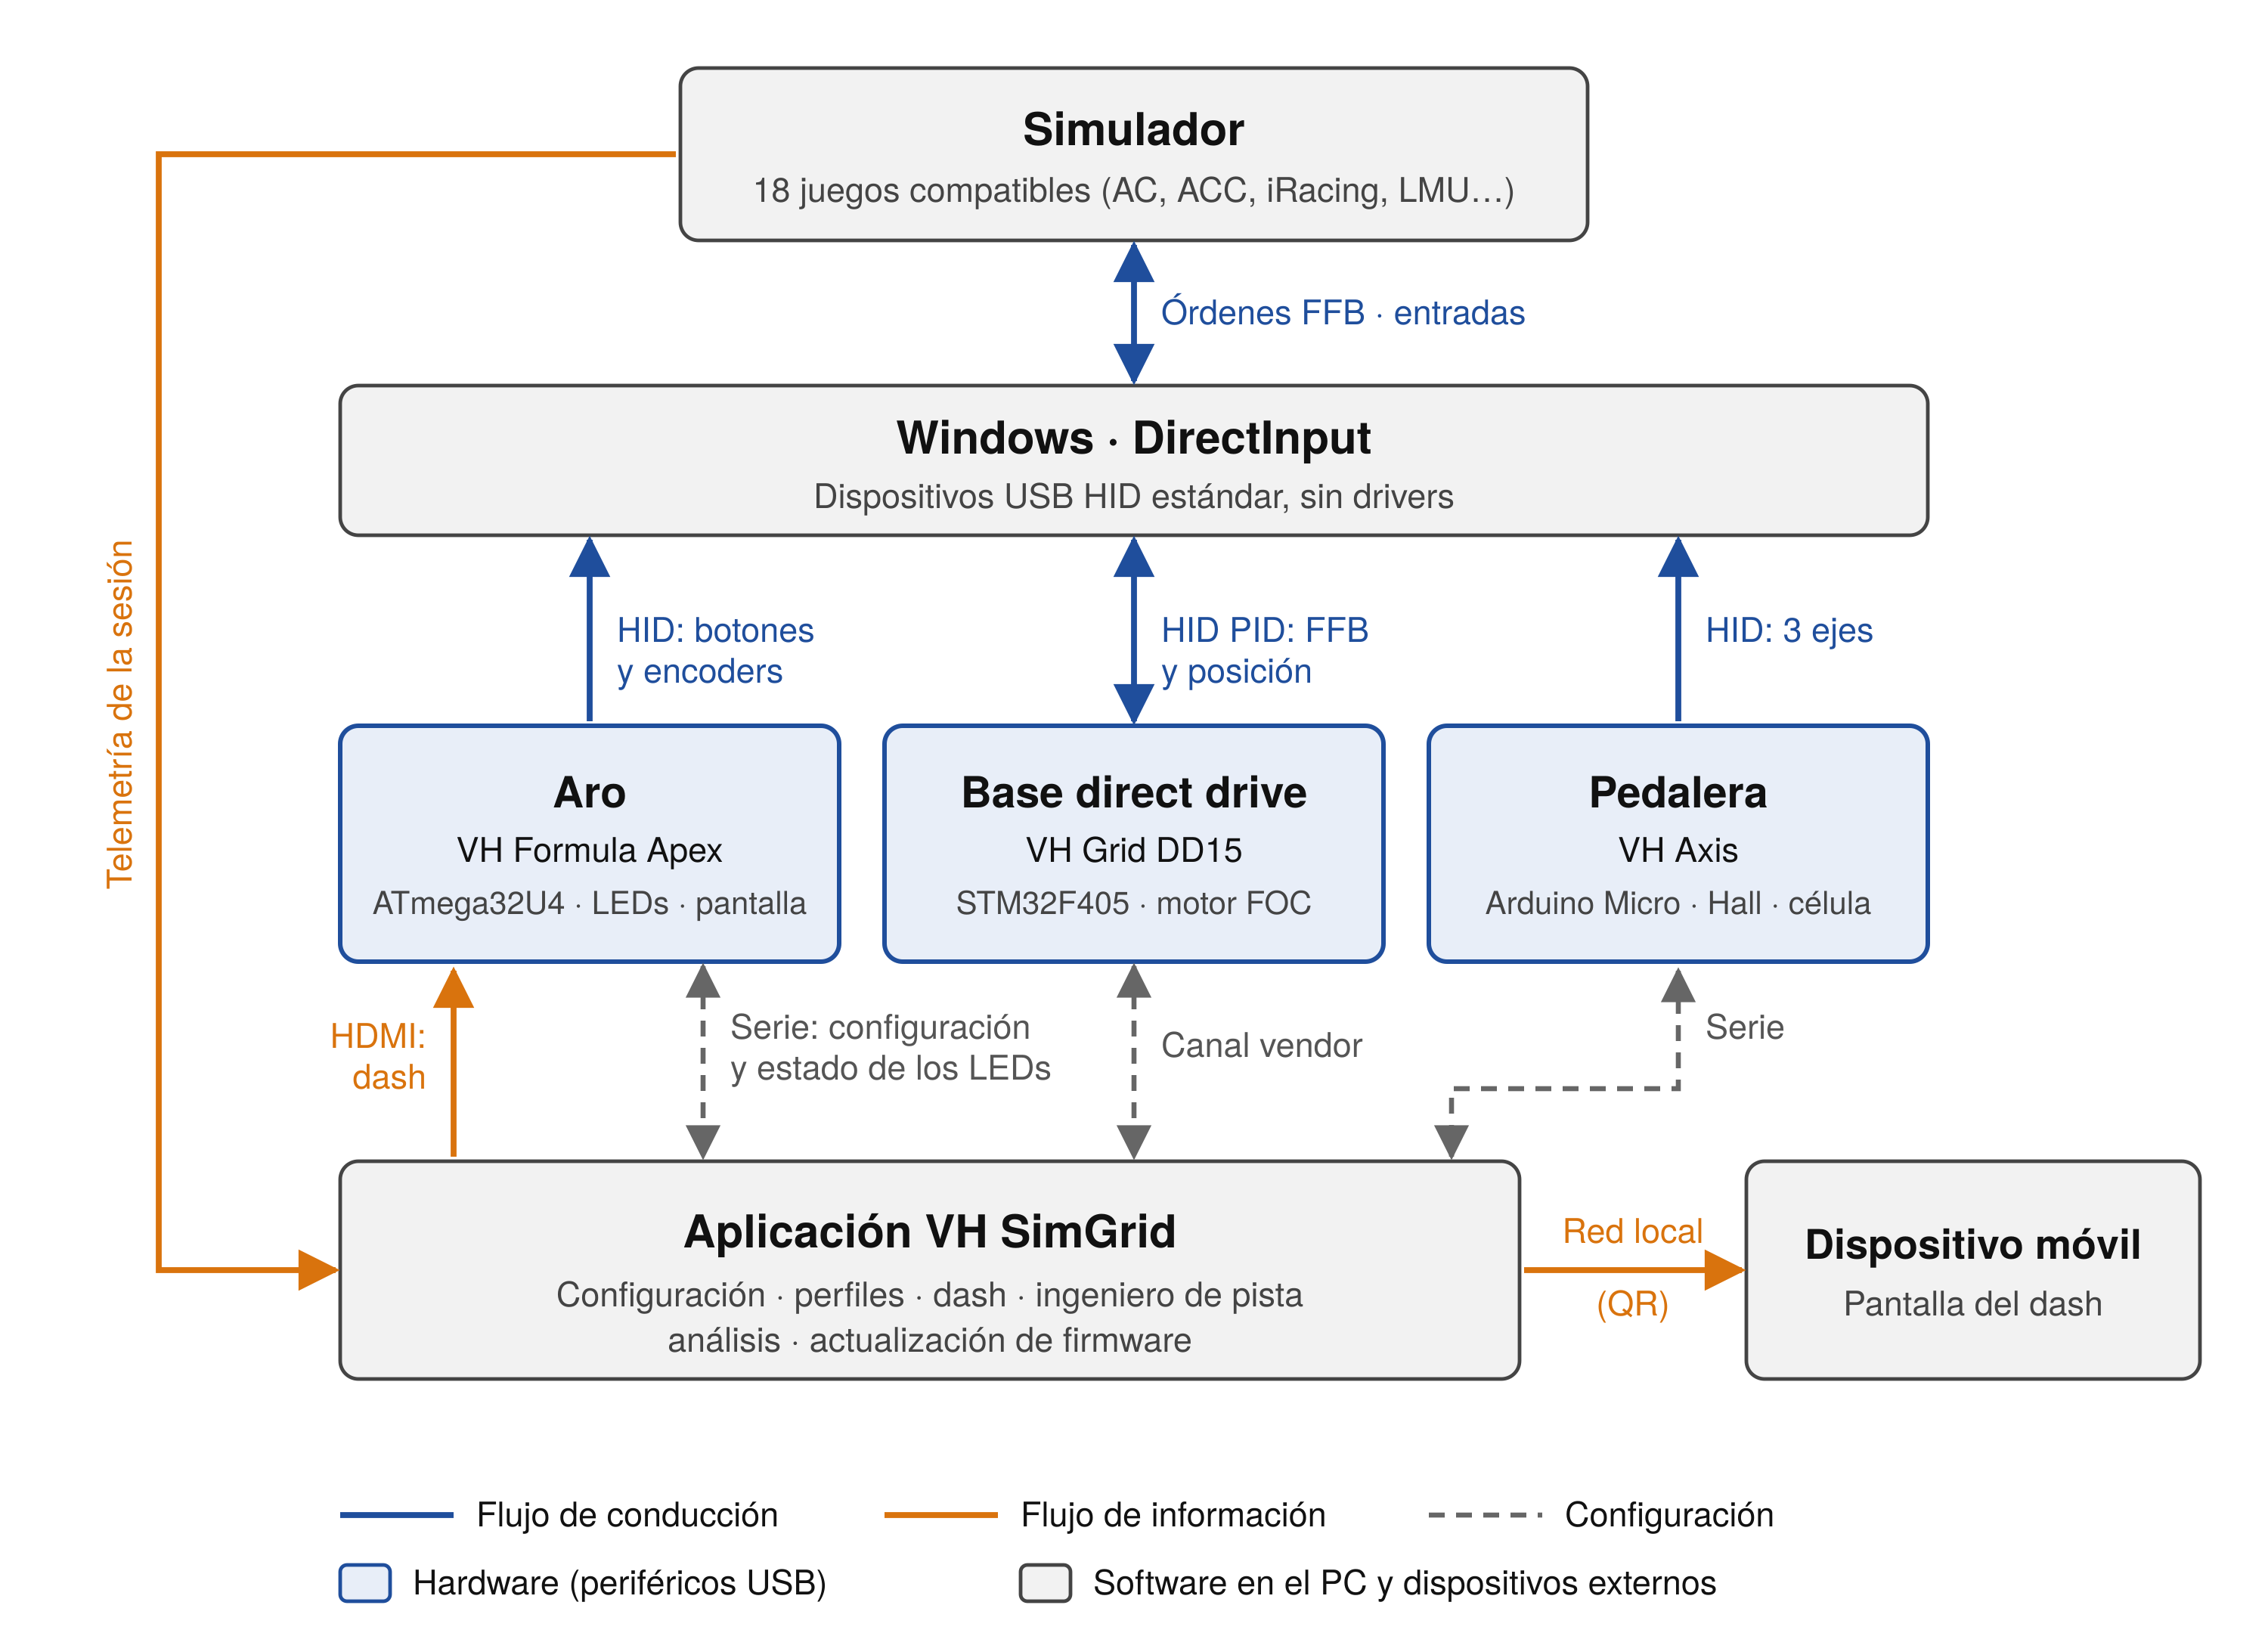
\includegraphics[width=0.84\textwidth,trim=141 39 87 87,clip]{img/diagrama-bloques.png}
	\caption{Diagrama de bloques del ecosistema VH SimGrid. (Fuente propia)}
	\label{fig:diagrama-bloques}
\end{figure}

El diseño separa dos flujos que en la práctica circulan a la vez. El \textbf{flujo de conducción} va del simulador a los periféricos y de los periféricos al simulador, a través de Windows: las órdenes de force feedback, los ejes de los pedales y los botones del aro. El \textbf{flujo de información} va del simulador a la aplicación y de ella al piloto: la telemetría, los LEDs, el dash en la pantalla del aro y en el dispositivo móvil, y la voz del ingeniero. El primero es crítico en tiempo y en seguridad; el segundo enriquece la experiencia. Esta separación es la base del reparto de responsabilidades que se describe a continuación. El detalle de cada canal se recoge en la sección~\ref{sec:protocolos}.

\subsection{Reparto de responsabilidades}
\label{subsec:reparto-responsabilidades}
El principio que guía el diseño es que \textbf{el hardware funciona sin la aplicación abierta}. Cada periférico es autónomo en todo lo necesario para conducir: guarda su propia configuración y se comunica directamente con el simulador a través de los mecanismos estándar de Windows. La aplicación no forma parte del flujo de conducción. Configura los periféricos y añade funciones sobre ellos, pero no es un intermediario por el que deban pasar los datos. Este principio responde directamente a los requisitos RNF19 y RNF20.

Esta decisión responde a tres motivos:

\begin{enumerate}
	\item \textbf{Latencia.} Las órdenes de force feedback viajan del simulador a la base sin pasar por la aplicación. Todo el procesado de la fuerza (curva, ecualizador, efectos base y rango de giro) se ejecuta en el propio firmware, en tiempo real.
	\item \textbf{Robustez y seguridad.} Un cierre inesperado de la aplicación no afecta a la conducción. Las protecciones de la base residen en su firmware y actúan siempre, con independencia del estado del ordenador.
	\item \textbf{Compatibilidad.} Al presentarse como dispositivos HID estándar, los periféricos funcionan en cualquier simulador compatible con DirectInput, incluidos los que la aplicación no admite para telemetría.
\end{enumerate}

En consecuencia, la aplicación se reserva tres tipos de funciones: las de \textbf{configuración} (ajustes en vivo, calibraciones, perfiles y actualización de firmware), las que \textbf{dependen de la telemetría} (los LEDs de revoluciones y eventos del aro, el dash en su pantalla, el ingeniero de pista y la grabación de sesiones) y las de \textbf{gestión} (perfiles automáticos por juego y por coche, y copias de seguridad). La tabla~\ref{tab:reparto-responsabilidades} detalla este reparto.

\begin{table}[H]
	\centering
	\caption{Reparto de responsabilidades entre los periféricos y la aplicación.}
	\label{tab:reparto-responsabilidades}
	\small
	\begin{tabularx}{\textwidth}{@{}>{\raggedright\arraybackslash}p{2.8cm}>{\raggedright\arraybackslash}X>{\raggedright\arraybackslash}X@{}}
		\toprule
		\textbf{Elemento} & \textbf{Funciona sin la aplicación} & \textbf{Requiere la aplicación} \\
		\midrule
		Base VH Grid DD15 &
		Force feedback nativo y efectos (constante, \emph{spring}, \emph{damper}, fricción e inercia); curva, ecualizador y rango de giro; anti-cogging; protecciones de seguridad; ajustes guardados en flash. &
		Modificar los ajustes; cambio automático de perfil; actualización de firmware. \\
		Pedalera VH Axis &
		Lectura de los tres pedales; calibración, curvas y zona muerta guardadas en EEPROM. &
		Calibración guiada; edición de curvas; traza en vivo; actualización de firmware. \\
		Aro VH Formula Apex &
		Botones y encoders como mando estándar; brillo guardado. &
		LEDs de revoluciones y eventos y dash en la pantalla HDMI, que dependen de la telemetría; configuración de luces; actualización de firmware. \\
		Aplicación VH SimGrid &
		--- &
		Telemetría, dash, ingeniero de pista, análisis de sesiones, perfiles y copias de seguridad. \\
		\bottomrule
	\end{tabularx}
\end{table}

Los únicos elementos del hardware que dependen por completo de la aplicación son la tira de LEDs y la pantalla del aro, ya que su contenido procede de la telemetría del simulador. Aun así, el aro sigue siendo plenamente funcional como mando aunque la aplicación no esté abierta.

\section{Diseño de componentes}
\label{sec:diseno-componentes}
Esta sección describe el diseño mecánico y electrónico de los tres periféricos. Para cada uno se recogen los requisitos que debe cumplir, los componentes electrónicos elegidos y el motivo de cada elección, el esquema de conexiones y el concepto mecánico. El proceso de fabricación y montaje de las piezas se detalla en el apartado~\ref{subsec:fabricacion}, y el firmware de cada periférico en la sección~\ref{sec:implementacion-componentes}.

\subsection{Criterios de diseño}
\label{subsec:criterios-diseno}
El diseño de los tres periféricos sigue unos mismos criterios, derivados de los requisitos y de las restricciones generales del capítulo~\ref{cap:requisitos}: un presupuesto propio, una sola persona y un taller doméstico.

\paragraph{Materiales baratos y fáciles de trabajar.}
La industria del automóvil no fabrica sus primeros prototipos con los materiales definitivos. Las formas de un coche nuevo se validan antes en maquetas de arcilla, espuma o madera, que se modelan y corrigen con rapidez y a bajo coste, y solo cuando la forma está decidida se pasa a los materiales y procesos de producción. Este trabajo adopta el mismo enfoque. Cada pieza se valida primero en materiales baratos y fáciles de trabajar, comenzando por poliestireno expandido de alta densidad, después madera y por último PLA impreso en 3D, que permiten comprobar dimensiones, ergonomía y ajustes con muy poca inversión. Solo cuando la pieza está validada se fabrica en su material final, el ABS, más resistente a los esfuerzos y a la temperatura, con un acabado superficial que imita la fibra de carbono. Además, las piezas de acabado liso se tratan con vapor de acetona para conseguir una superficie totalmente pulida.

\paragraph{Componentes comerciales al por menor.}
Toda la electrónica se compone de módulos y componentes que se pueden comprar en tiendas de electrónica o en línea, sin pedidos mínimos ni piezas a medida. Siempre que existe, se elige una plataforma abierta y documentada, como la controladora ODrive o los microcontroladores compatibles con Arduino, de modo que el firmware pueda adaptarse sin depender de un fabricante. Este criterio es el que permite cumplir los requisitos de coste RNF16 y RNF17.

\subsection{Aro VH Formula Apex}
\label{subsec:diseno-aro}
\paragraph{Requisitos.}
El aro debe reunir los mandos que el piloto usa durante la conducción (RF16 y RF17), una tira de LEDs para las revoluciones y los eventos de carrera (RF18 a RF21) y una pantalla en la que se reproduzca el \textit{dash} y desde la que se pueda configurar el equipo (RF22 a RF28). Todo ello debe caber en el espacio reducido de un volante de tipo Fórmula y con un peso contenido, porque toda la masa del aro la tiene que mover el motor de la base y empeora la respuesta del \textit{force feedback}.

La pantalla añade sus propias condiciones (RNF31 a RNF37): una diagonal de entre 4 y 7 pulgadas, integrada sin tapar la visión de la pista ni estorbar a las manos, los botones o las palancas; un peso inferior a 300~g junto con su soporte; una resolución mínima de $800\times480$ píxeles en un panel IPS o equivalente; alimentación por USB, sin fuente adicional; un cableado que soporte el giro completo del volante y el desmontaje rápido del aro; y resistencia a las vibraciones del \textit{force feedback}.

\paragraph{Electrónica.}
El aro se organiza alrededor de un microcontrolador ATmega32U4. Su principal ventaja es el USB integrado, que le permite presentarse a la vez como mando HID, para los botones, y como puerto serie, para la configuración y el estado de los LEDs. Un volante de tipo Fórmula necesita muchos mandos en poco espacio, y el microcontrolador no tiene pines suficientes para leerlos uno a uno. Por eso los pulsadores se leen en matriz, que reduce el número de pines necesarios a la suma de filas y columnas, y los \textit{encoders} se conectan a través de un expansor de entradas y salidas MCP23017 por el bus I2C. La tira de LEDs es de tipo WS2812, en la que cada LED integra su propio controlador y se gobierna individualmente con una única línea de datos.

La pantalla es la excepción: no se conecta al microcontrolador, sino directamente al ordenador por HDMI, como un monitor más que Windows reconoce sin controladores (RF22), y se alimenta por USB (RNF36). Generar el \textit{dash} en el microcontrolador obligaría a usar un procesador mucho más potente y limitaría lo que puede mostrarse. Usando la pantalla como un monitor, el \textit{dash} lo dibuja la aplicación con toda la potencia del ordenador, y el aro solo aporta el panel. La tabla~\ref{tab:componentes-aro} resume los componentes y la figura~\ref{fig:esquema-aro} muestra sus conexiones.

\begin{table}[H]
	\centering
	\caption{Componentes electrónicos del aro VH Formula Apex.}
	\label{tab:componentes-aro}
	\small
	\begin{tabularx}{\textwidth}{@{}>{\raggedright\arraybackslash}p{3.2cm}>{\raggedright\arraybackslash}p{3.6cm}X@{}}
		\toprule
		\textbf{Componente} & \textbf{Función} & \textbf{Motivo de la elección} \\
		\midrule
		Microcontrolador ATmega32U4 & Lee los mandos, gobierna los LEDs y se comunica con el PC & USB nativo, que permite ser mando HID y puerto serie a la vez sin hardware adicional. \\
		Matriz de pulsadores & Botones del aro & Lee muchos pulsadores con pocos pines. \\
		Expansor MCP23017 & Lectura de los \textit{encoders} & Añade entradas por I2C sin ocupar pines del microcontrolador. \\
		Tira de LEDs WS2812 & Barra de RPM y luces por eventos & Cada LED se controla por separado en color y brillo con una sola línea de datos. \\
		Palancas de embrague & Embrague manual desde el aro & Permiten las salidas con punto de mordida (RF17). \\
		Pantalla HDMI & Reproduce el \textit{dash} y el menú de configuración & Se conecta al PC como un monitor y se alimenta por USB; el \textit{dash} lo dibuja la aplicación. \\
		\bottomrule
	\end{tabularx}
\end{table}
\begin{figure}[H]
	\centering
	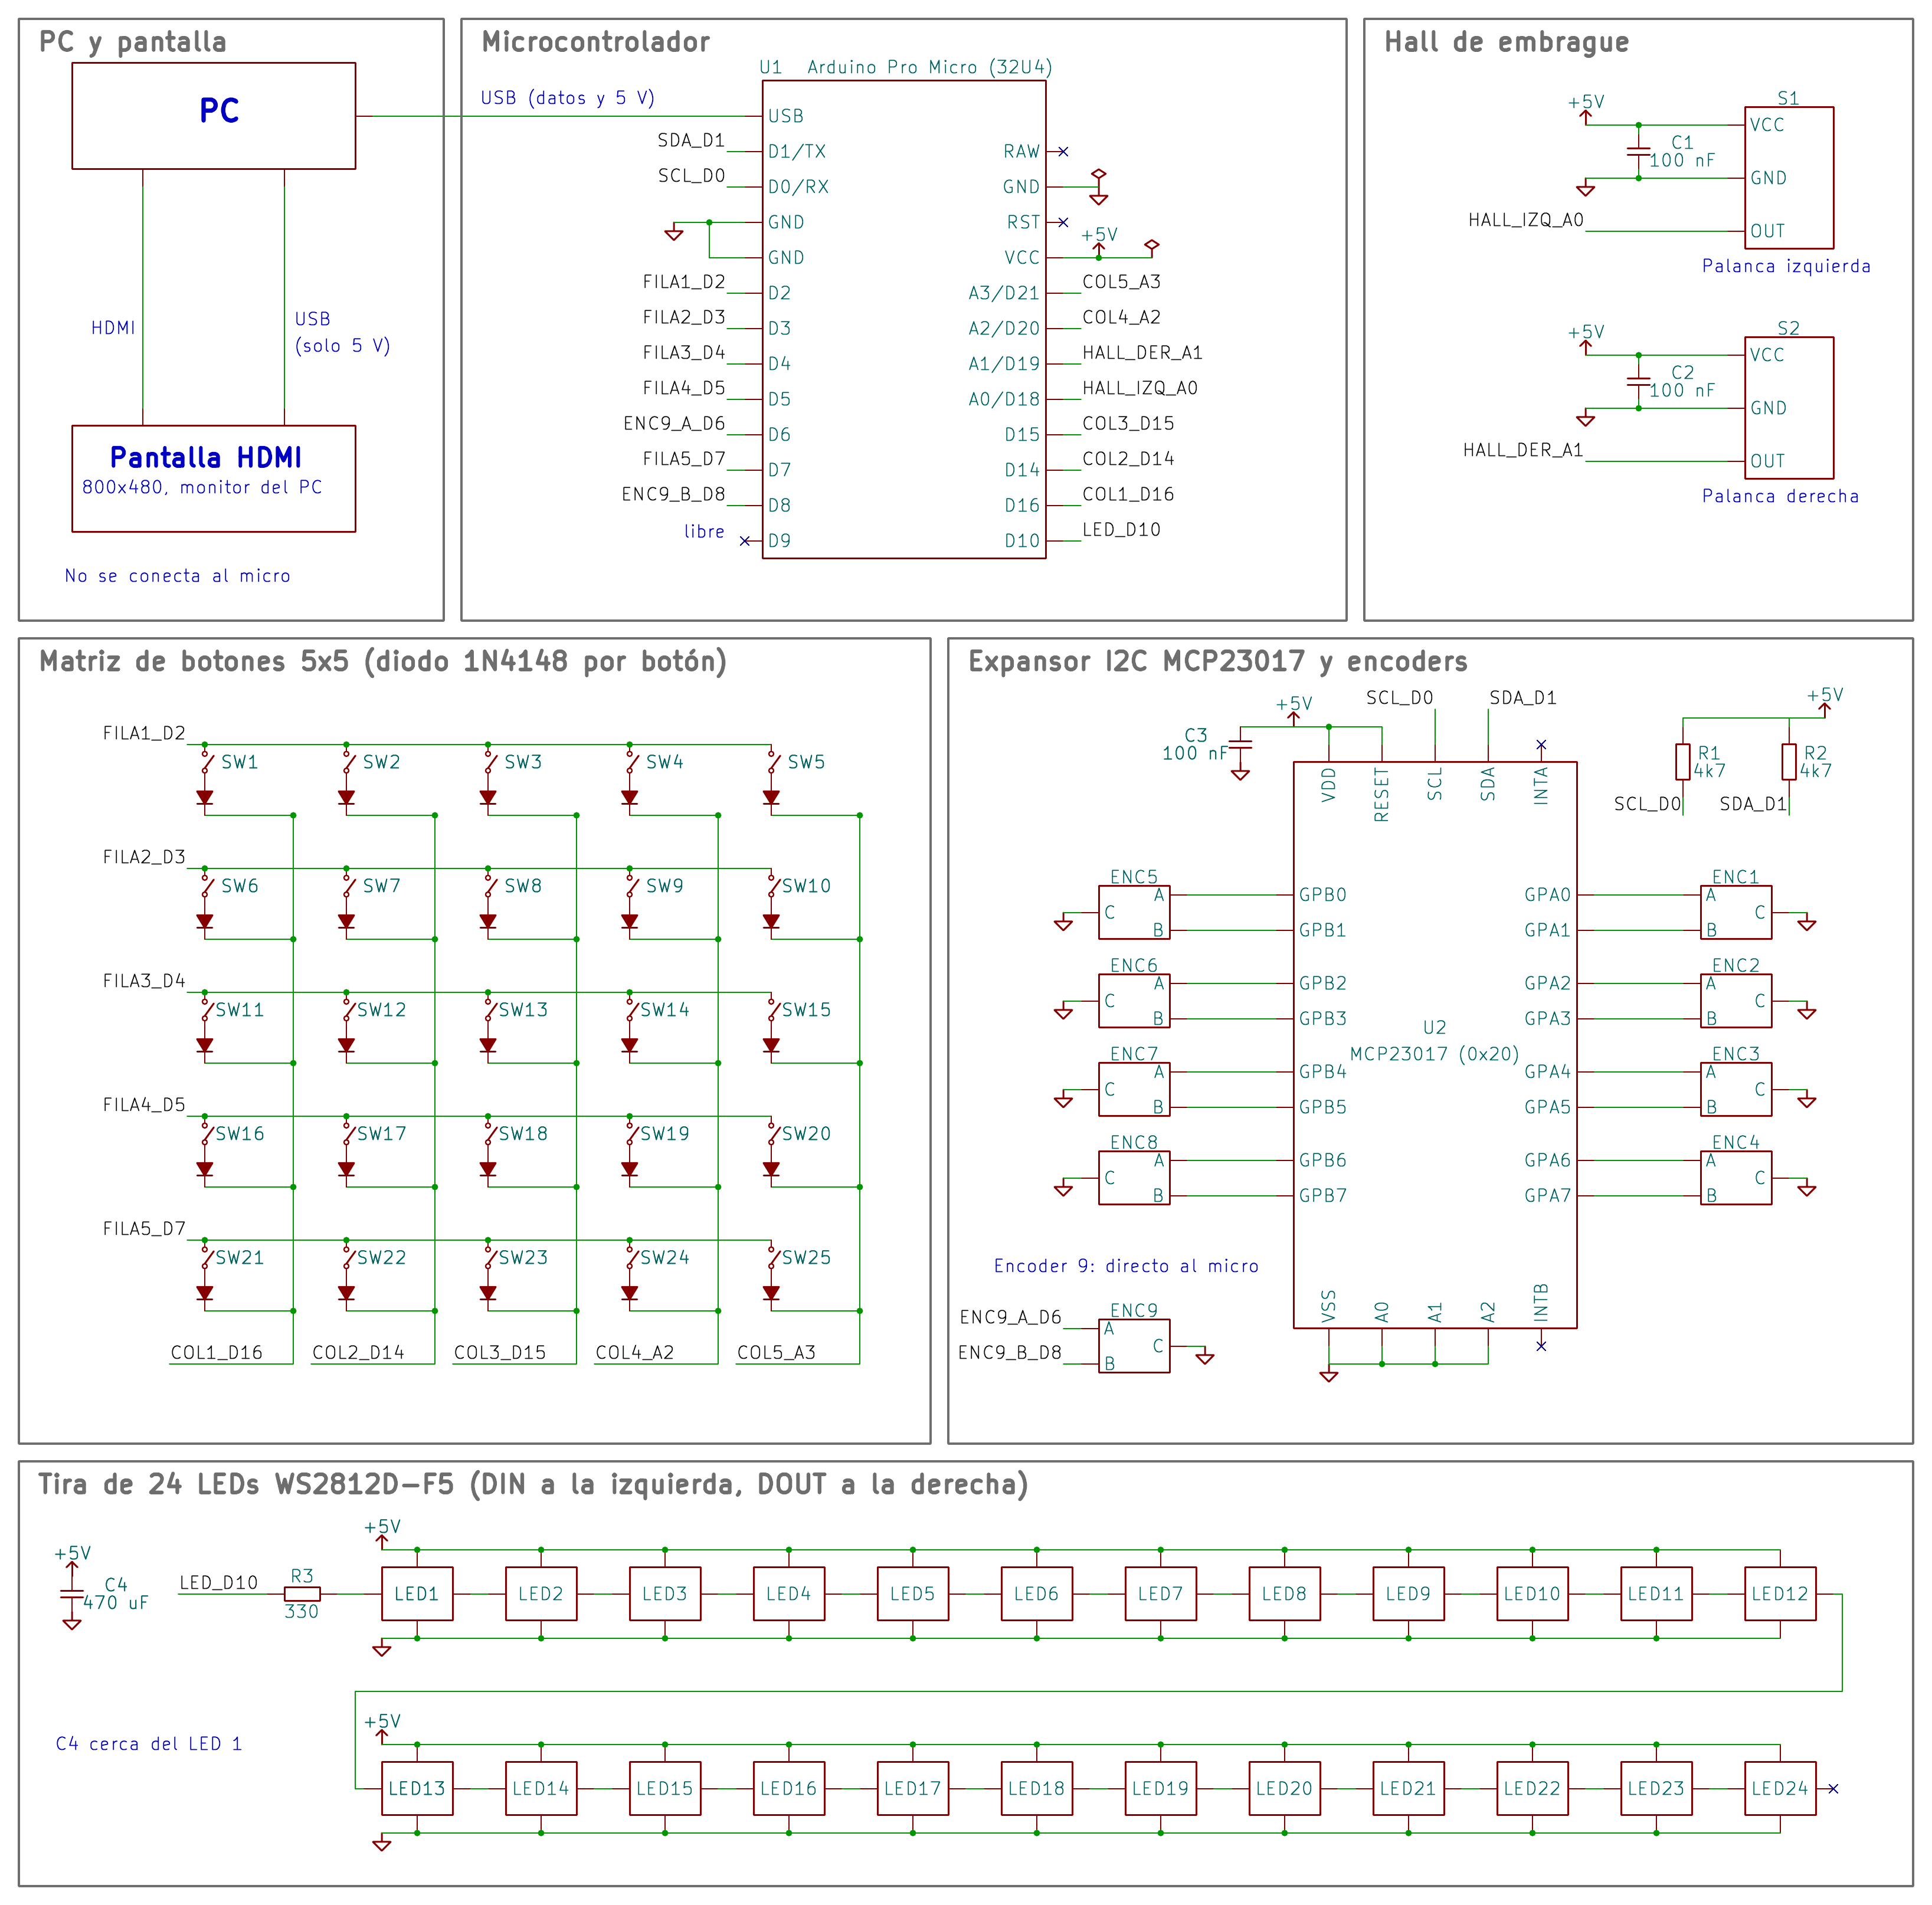
\includegraphics[width=\textwidth]{img/aro-esquema.png}
	\caption{Esquema de conexiones del aro VH Formula Apex. (Fuente propia)}
	\label{fig:esquema-aro}
\end{figure}

\paragraph{Concepto mecánico.}
El aro sigue la forma de los volantes de los monoplazas actuales, los cuales se caracterizan por su pequeño diámetro, con dos empuñaduras laterales y los mandos concentrados en el frontal, alrededor de la pantalla, para que el piloto los alcance con los pulgares sin soltar las manos. La pantalla ocupa el centro del frontal, a la altura de la vista pero por debajo de la línea de visión hacia la pista (RNF31), y su soporte forma parte del propio cuerpo del aro para resistir las vibraciones (RNF37). La tira de LEDs se sitúa en la parte superior, en la línea de visión del piloto hacia la pista. Las levas de cambio y las palancas de embrague van en la parte trasera, al alcance de los dedos. El cuerpo se divide en piezas que alojan la electrónica en su interior, y el aro se une a la base mediante un sistema de desmontaje rápido por el que pasan también los cables de USB y HDMI (RNF35). La figura~\ref{fig:render-aro} muestra el diseño.

\begin{figure}[H]
	\centering
	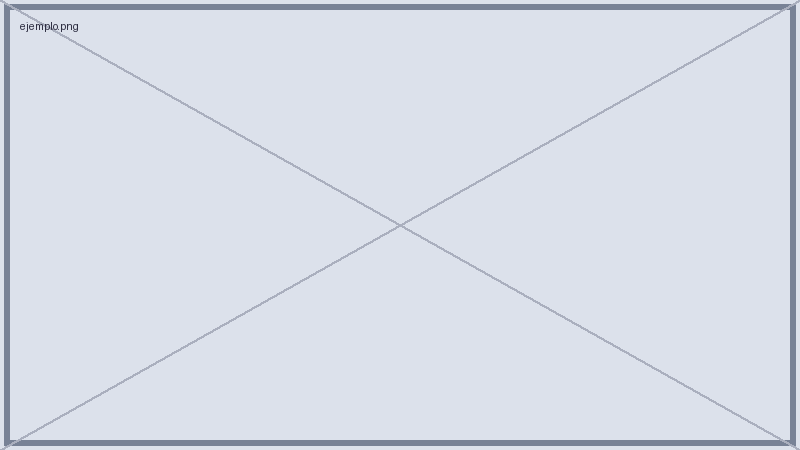
\includegraphics[width=0.8\textwidth]{img/ejemplo.png}
	\caption{Diseño del aro VH Formula Apex. (Fuente propia)}
	\label{fig:render-aro}
\end{figure}

\subsection{Pedalera VH Axis}
\label{subsec:diseno-pedalera}
\paragraph{Requisitos.}
La pedalera debe presentarse como un mando de tres ejes, con el acelerador y el embrague medidos por posición y el freno por fuerza (RF11), y guardar su configuración en su propia memoria (RF14 y RNF19). Debe leer los pedales a unos 1000~Hz sin un retardo perceptible (RNF3). Mecánicamente, el freno debe soportar de forma repetida la fuerza máxima de la célula de carga sin deformarse ni perder la calibración (RNF23).

\paragraph{Electrónica.}
La pedalera usa un Arduino Micro, que monta el mismo ATmega32U4 que el aro y comparte con él la ventaja del USB nativo, es mando HID de tres ejes y puerto serie de configuración a la vez. El acelerador y el embrague miden su recorrido con sensores de efecto Hall, que detectan la posición de un imán sin contacto y no se desgastan. Su salida es analógica y se lee directamente con el conversor del microcontrolador.

El freno mide la fuerza con una célula de carga de 200~kg. Su señal es del orden de milivoltios y necesita amplificarse antes de digitalizarla. La solución habitual en proyectos de este tipo es el módulo HX711, un conversor de alta resolución pensado para básculas, pero su frecuencia de muestreo máxima, de 80 muestras por segundo, es muy inferior a los 1000~Hz que exige el requisito RNF3. Por eso, y tras las pruebas realizadas, se ha decidido usar en su lugar un amplificador de instrumentación INA333, que amplifica la señal del puente de la célula de forma continua y la entrega al conversor del microcontrolador, que puede leerla a la misma frecuencia que los otros dos pedales. La resolución que se pierde frente al HX711 se compensa con el filtrado digital de la señal. La tabla~\ref{tab:componentes-pedalera} resume los componentes y la figura~\ref{fig:esquema-pedalera} muestra sus conexiones.

\begin{table}[H]
	\centering
	\caption{Componentes electrónicos de la pedalera VH Axis.}
	\label{tab:componentes-pedalera}
	\small
	\begin{tabularx}{\textwidth}{@{}>{\raggedright\arraybackslash}p{3.2cm}>{\raggedright\arraybackslash}p{3.6cm}X@{}}
		\toprule
		\textbf{Componente} & \textbf{Función} & \textbf{Motivo de la elección} \\
		\midrule
		Arduino Micro (ATmega32U4) & Lee los sensores y se comunica con el PC & USB nativo, que permite ser mando HID y puerto serie a la vez. \\
		Sensores de efecto Hall & Recorrido del acelerador y del embrague & Miden sin contacto, sin desgaste ni ruido mecánico. \\
		Célula de carga de 200~kg & Fuerza sobre el freno & Mide la magnitud que controla el piloto en una frenada real. \\
		Amplificador INA333 & Amplifica la señal de la célula & Permite leer el freno a unos 1000~Hz, frente a las 80 muestras por segundo del HX711. \\
		\bottomrule
	\end{tabularx}
\end{table}
\begin{figure}[H]
	\centering
	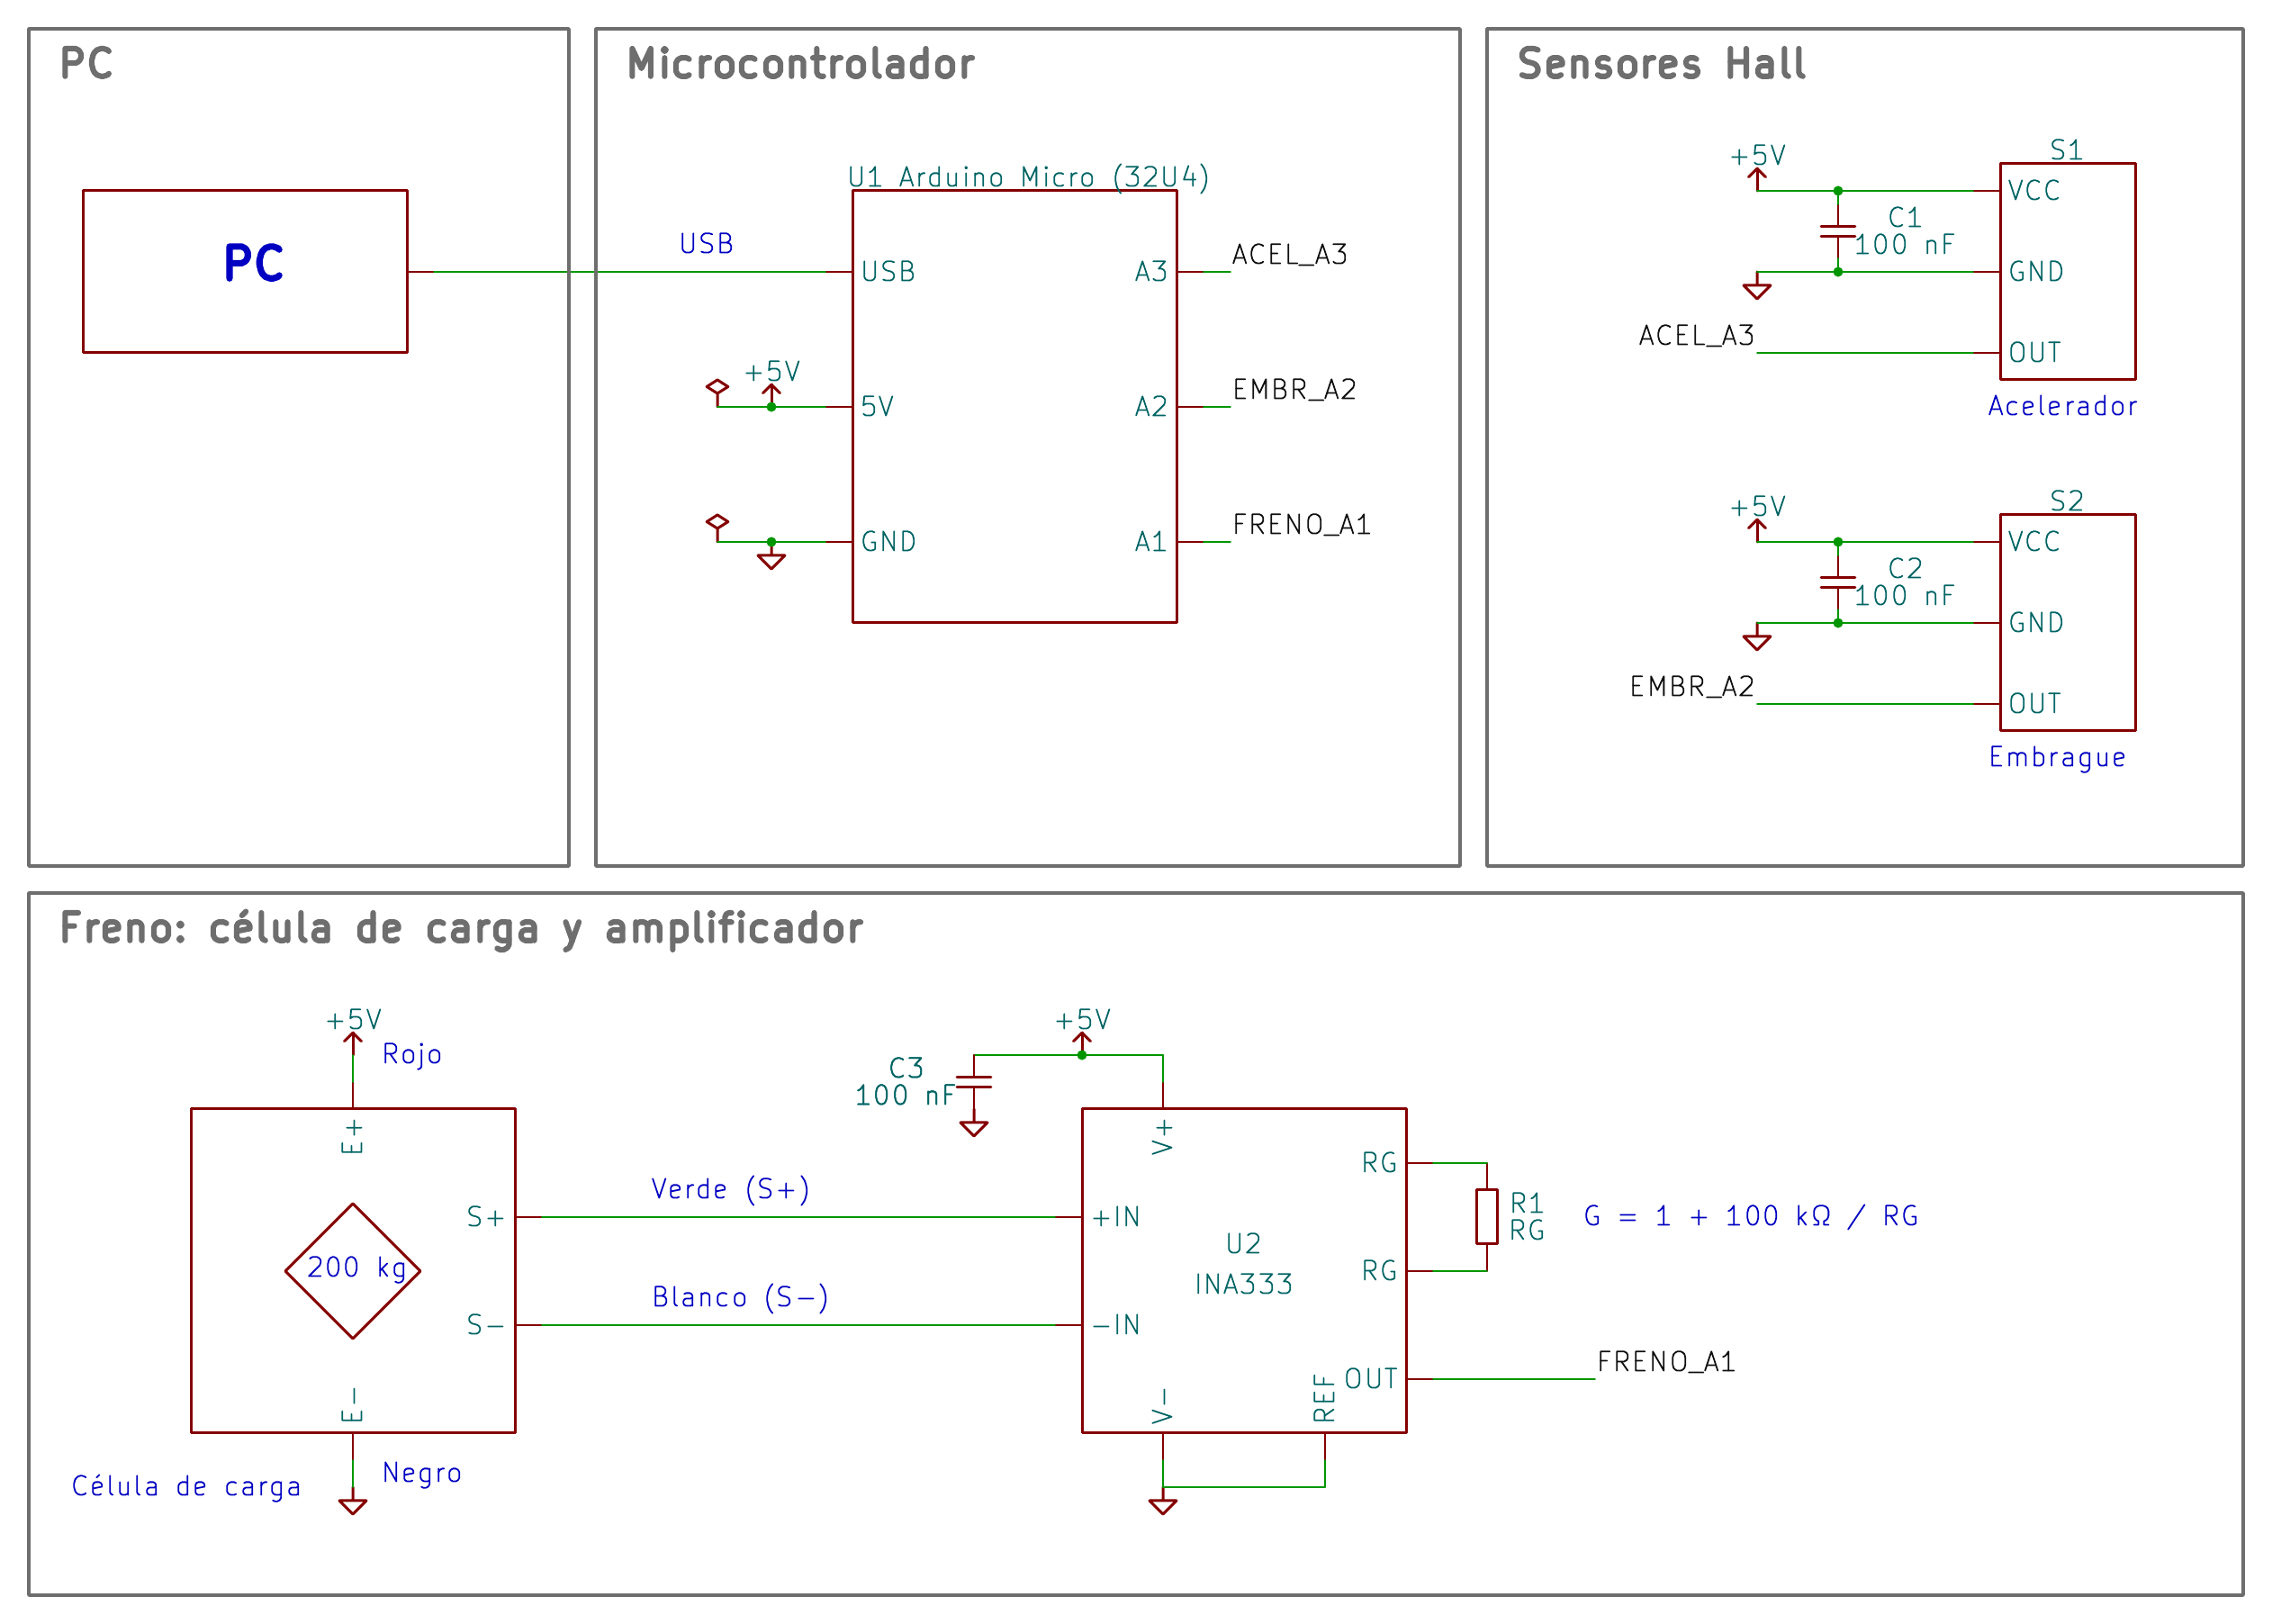
\includegraphics[width=\textwidth]{img/pedalera-esquema.png}
	\caption{Esquema de conexiones de la pedalera VH Axis. (Fuente propia)}
	\label{fig:esquema-pedalera}
\end{figure}

\paragraph{Concepto mecánico.}
Cada pedal es un brazo que gira sobre un eje fijado a la base de la pedalera, con su sensor en el propio pivote o en el recorrido del brazo. El acelerador y el embrague recuperan su posición con un muelle, porque lo que importa en ellos es el recorrido. En el freno, en cambio, el pedal apenas debe moverse: el brazo empuja contra la célula de carga a través de un elemento elástico que le da una resistencia progresiva, de modo que el pie sienta una dureza creciente parecida a la de un freno hidráulico. El brazo del freno y su apoyo sobre la célula se dimensionan para la fuerza máxima de esta, de modo que una frenada a fondo no deforme la estructura ni desplace la célula (RNF23). Los tres pedales se montan sobre una base común, con la separación y la inclinación de un pedalier de competición. La figura~\ref{fig:render-pedalera} muestra el diseño.

\begin{figure}[H]
	\centering
	% TODO: render CAD de la pedalera
	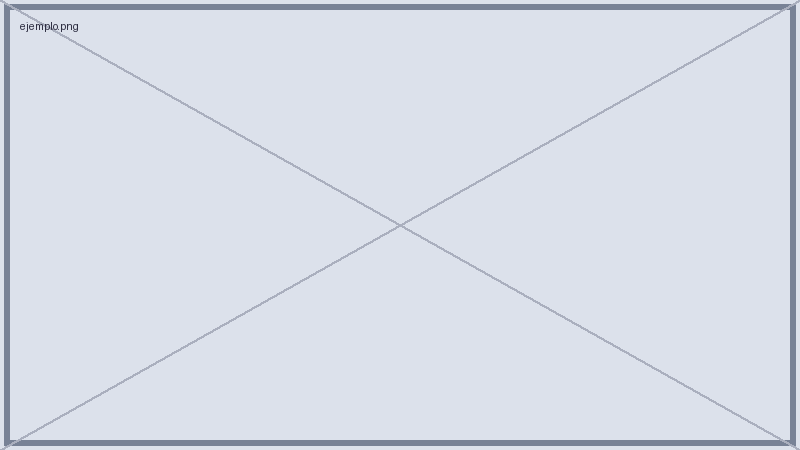
\includegraphics[width=0.8\textwidth]{img/ejemplo.png}
	\caption{Diseño de la pedalera VH Axis. (Fuente propia)}
	\label{fig:render-pedalera}
\end{figure}
% TODO: elemento elástico del freno (elastómero, muelles...) y material de la estructura y los brazos.

\subsection{Base VH Grid DD15}
\label{subsec:diseno-base}

\paragraph{Requisitos.}
La base debe ser reconocida como un volante con \textit{force feedback} nativo (RF1), reproducir los efectos de DirectInput (RF2) y ofrecer un rango de giro de hasta 1440° (RF3). Debe atender los informes de fuerza cada milisegundo y aplicar el par en menos de 2~ms desde que llegan (RNF1 y RNF2). Por encima de todo, debe ser segura: un motor capaz de mover el volante con fuerza puede lesionar al piloto si el control falla, por lo que la electrónica debe permitir vigilar en todo momento la velocidad, la corriente y la temperatura del motor y de la controladora, y cortar el par ante cualquier anomalía (RNF8 a RNF14).

\paragraph{Electrónica.}
La base usa una transmisión \textit{direct drive}, en la que el aro va unido directamente al motor, sin engranajes ni correas que filtren o retrasen la fuerza. Esto exige un motor que dé mucho par a baja velocidad. El motor de buje de un patinete eléctrico cumple ese requisito: es un motor sin escobillas pensado para mover la rueda directamente, con muchos polos y un par elevado a pocas revoluciones, y su precio es una fracción del de los motores de las bases comerciales. Su inconveniente es un rizado magnético (\textit{cogging}) apreciable, que se nota en las manos como pequeños escalones al girar. En lugar de buscar un motor más caro, se decide corregirlo por software con una calibración anti-cogging (RF8), que se describe en el apartado~\ref{subsec:fw-base}.

Para controlar el motor se usa una controladora MKS ODrive Mini, compatible con el proyecto de código abierto ODrive. Integra un microcontrolador STM32F405, con USB nativo y potencia de cálculo suficiente para ejecutar el control vectorial (FOC) del motor y, a la vez, el dispositivo HID PID y el motor de efectos, de modo que toda la base funciona con una sola placa. La posición del volante se mide con un encoder óptico de alta resolución, necesario para el control FOC y para que la fuerza se calcule con precisión incluso en movimientos muy pequeños. El motor no lleva sonda de temperatura: el firmware estima su calentamiento a partir de la corriente aplicada (modelo I$^2$t) y reduce el par de forma progresiva antes de que se sobrecaliente. La temperatura de los transistores de la controladora sí se mide, con el termistor NTC que integra la placa (RNF9). La fuente de alimentación se dimensiona para la corriente de pico de la controladora, y la energía que el motor devuelve al frenar se limita para no dañarla (RNF11). La tabla~\ref{tab:componentes-base} resume los componentes y la figura~\ref{fig:esquema-base} muestra sus conexiones.

\begin{table}[H]
	\centering
	\caption{Componentes electrónicos de la base VH Grid DD15.}
	\label{tab:componentes-base}
	\small
	\begin{tabularx}{\textwidth}{@{}>{\raggedright\arraybackslash}p{3.2cm}>{\raggedright\arraybackslash}p{3.6cm}X@{}}
		\toprule
		\textbf{Componente} & \textbf{Función} & \textbf{Motivo de la elección} \\
		\midrule
		Motor de buje de patinete eléctrico & Genera el par sobre el volante & Mucho par a baja velocidad y muy bajo coste; su \textit{cogging} se corrige por software. \\
		Controladora MKS ODrive Mini (STM32F405) & Control FOC del motor, HID PID y efectos & Plataforma abierta, USB nativo y potencia para todo el firmware en una sola placa. \\
		Encoder óptico & Posición del volante & Alta resolución, necesaria para el control FOC y la precisión de la fuerza. \\
		Termistor NTC (integrado en la controladora) & Temperatura de los transistores & Permite limitar la corriente si la placa se calienta (RNF9). \\
		Fuente de alimentación & Alimenta la controladora y el motor & Dimensionada para la corriente de pico de la controladora. \\
		\bottomrule
	\end{tabularx}
\end{table}

\begin{figure}[H]
	\centering
	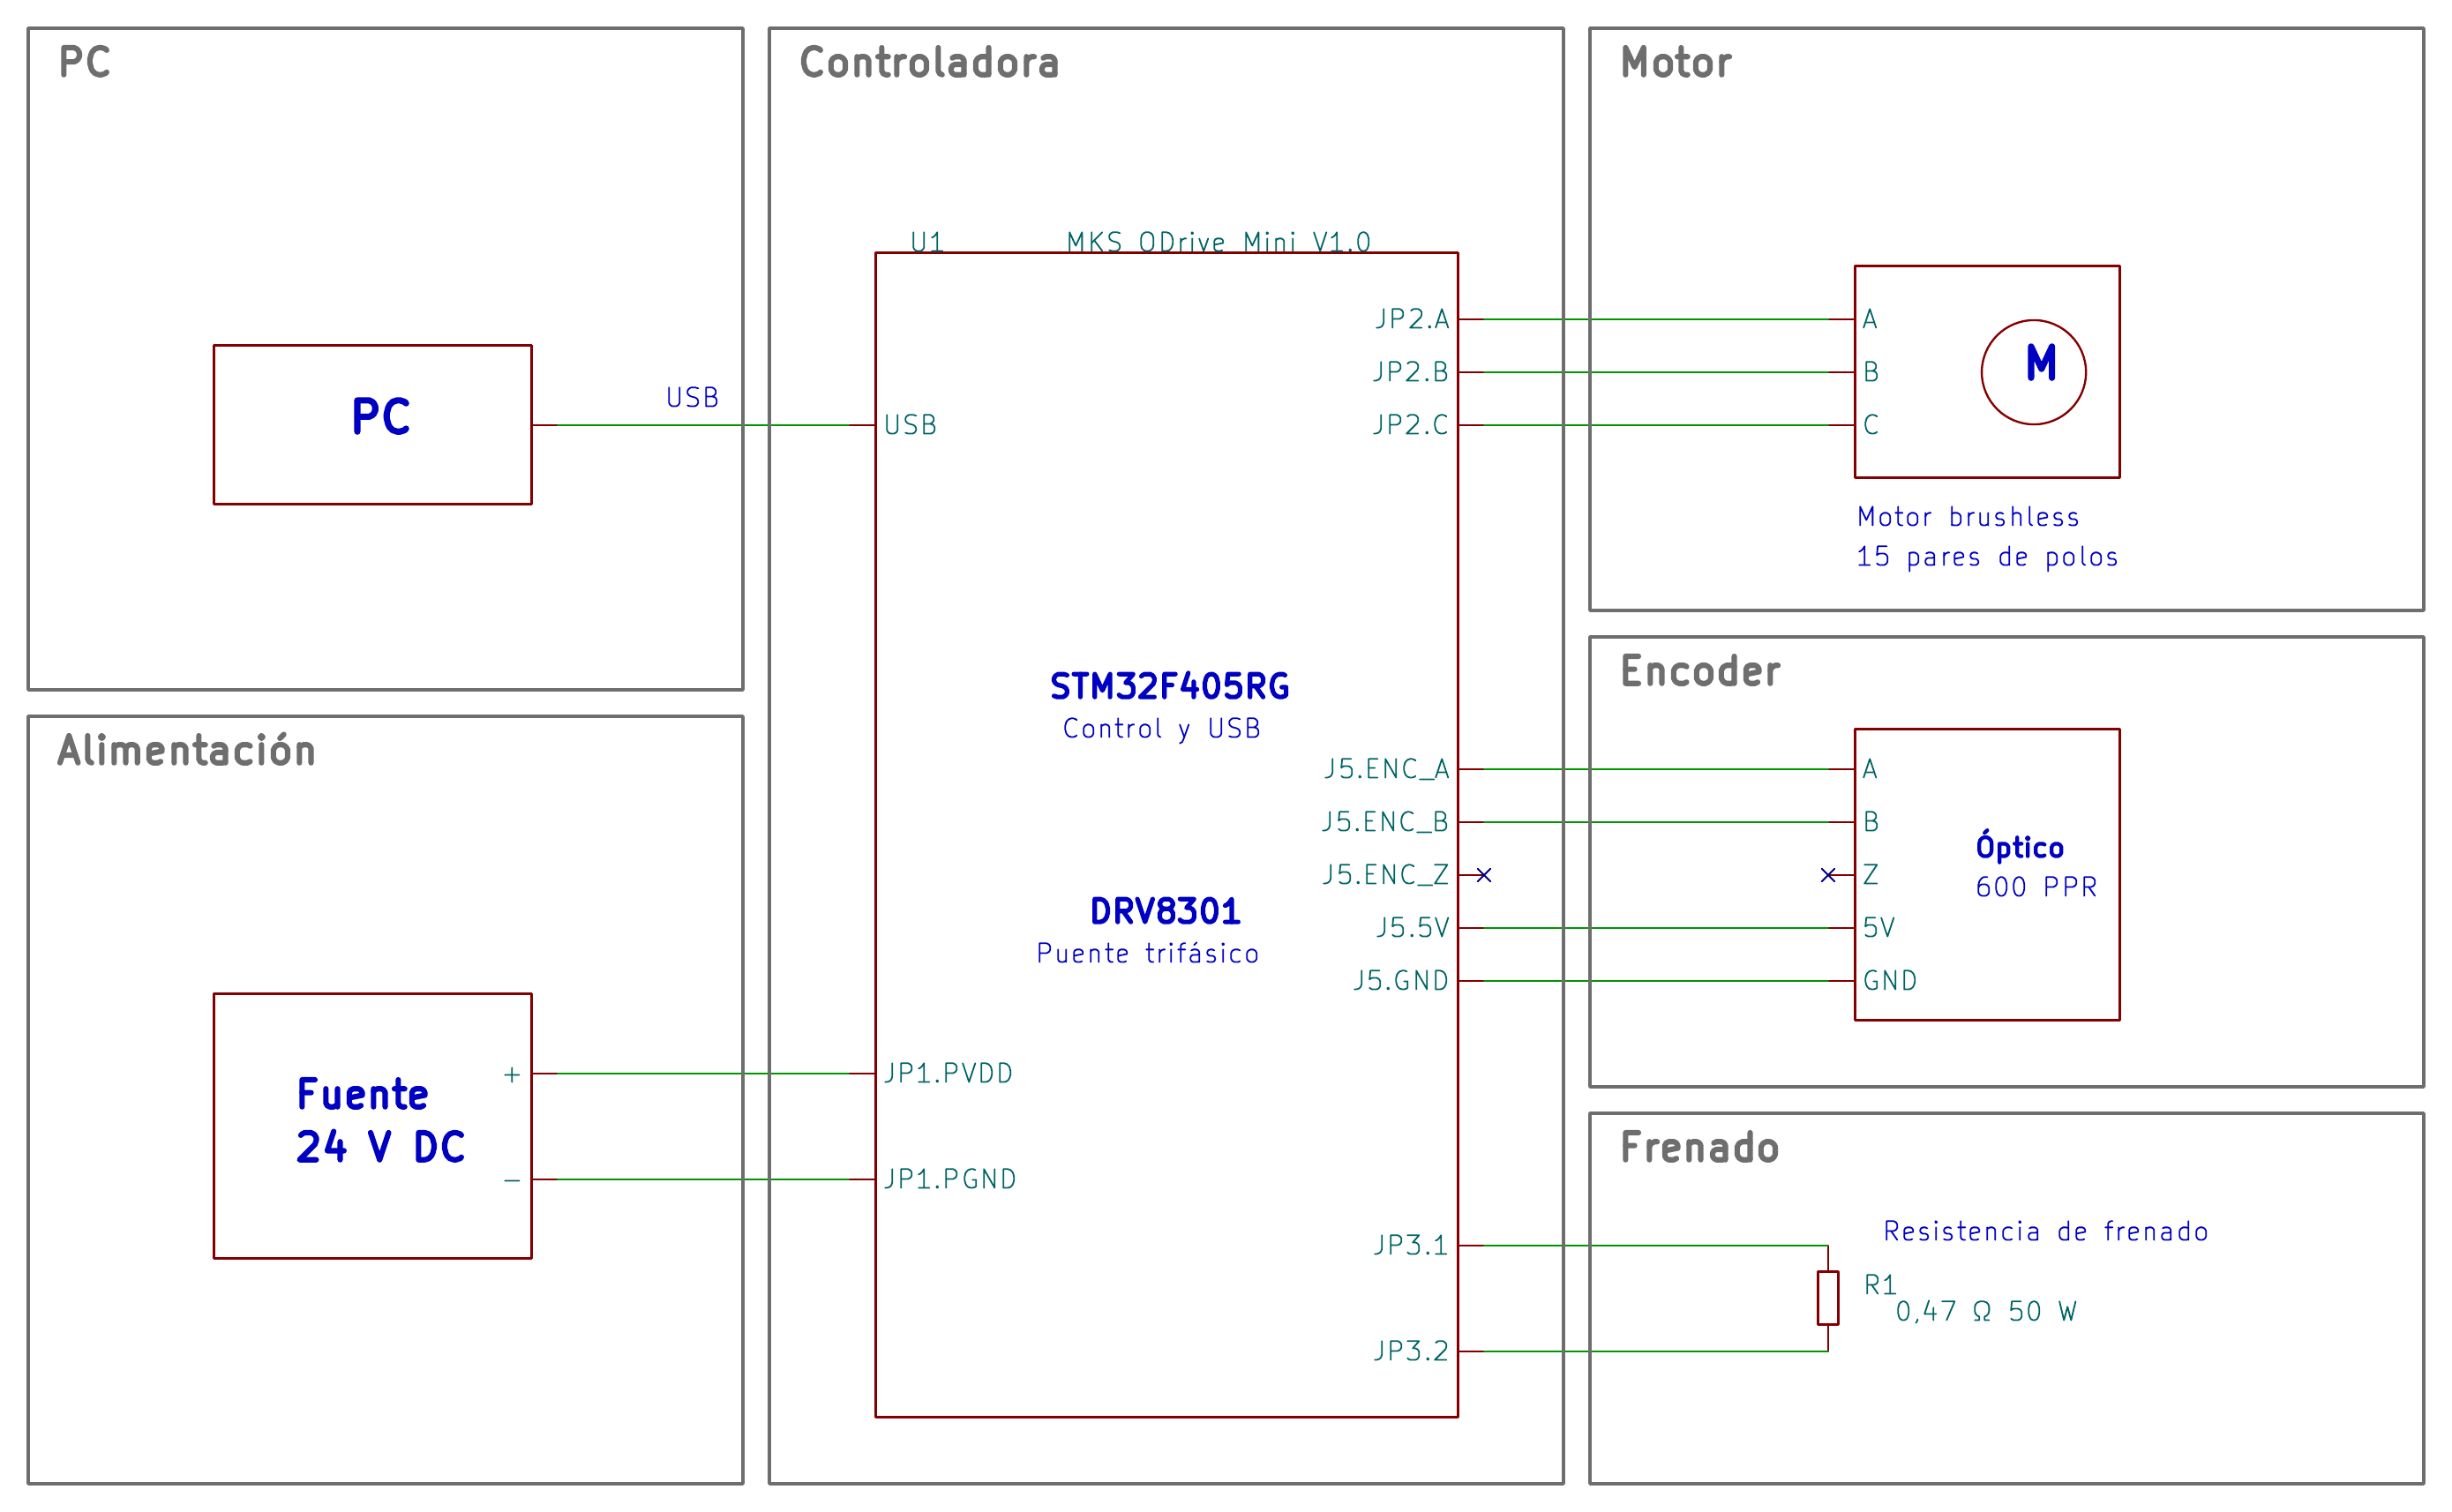
\includegraphics[width=\textwidth]{img/base-esquema.png}
	\caption{Esquema de conexiones de la base VH Grid DD15. (Fuente propia)}
	\label{fig:esquema-base}
\end{figure}

\paragraph{Concepto mecánico.}
En un motor de buje el eje es fijo y lo que gira es la carcasa exterior, que en el patinete es la propia rueda. El diseño aprovecha esta disposición: el eje del motor se fija a la estructura de la base y el aro se une a la carcasa giratoria mediante un adaptador con el sistema de desmontaje rápido, de modo que el par del motor llega al volante sin ningún elemento intermedio. La estructura aloja el motor, la controladora y el encoder, y se ancla con firmeza al puesto de conducción. La figura~\ref{fig:render-base} muestra el diseño.

\begin{figure}[H]
	\centering
	% TODO: render CAD de la base
	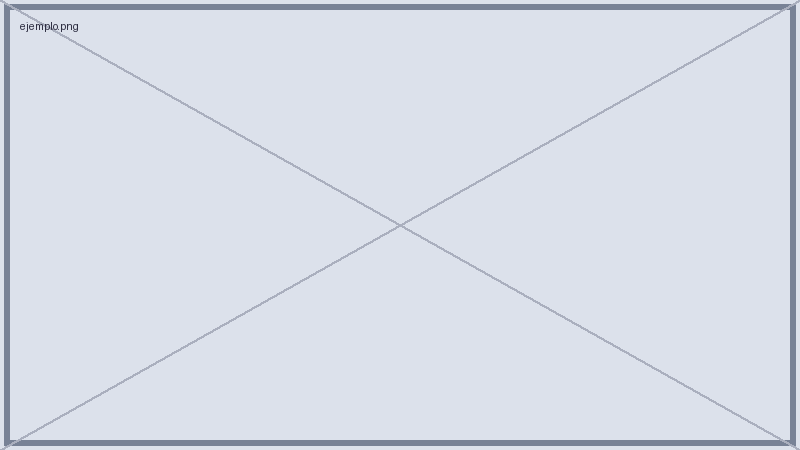
\includegraphics[width=0.8\textwidth]{img/ejemplo.png}
	\caption{Diseño de la base VH Grid DD15. (Fuente propia)}
	\label{fig:render-base}
\end{figure}

\section{Arquitectura tecnológica}
\label{sec:arquitectura-tecnologica}
El sistema tiene dos tipos de software: por un lado, el firmware que se ejecuta en cada periférico y, por otro, la aplicación de escritorio. Ambos se organizan en capas, de modo que cada capa solo depende de la que tiene debajo y ofrece sus servicios a la capa que tiene por encima. Esta separación permite cambiar una parte sin tocar el resto, por ejemplo sustituir un sensor afecta solo a la capa más baja del firmware, y añadir un simulador nuevo afecta solo al módulo de telemetría de la aplicación, como exige el requisito RNF43. Esta sección describe la organización de ambos.

\subsection{Firmware}
\label{subsec:arq-firmware}
Los tres periféricos comparten una misma estructura en capas, aunque cada uno la llena con funciones distintas según su papel. La figura~\ref{fig:capas-firmware} resume esta estructura y la tabla~\ref{tab:capas-firmware} describe la función de cada capa.

\begin{figure}[H]
	\centering
	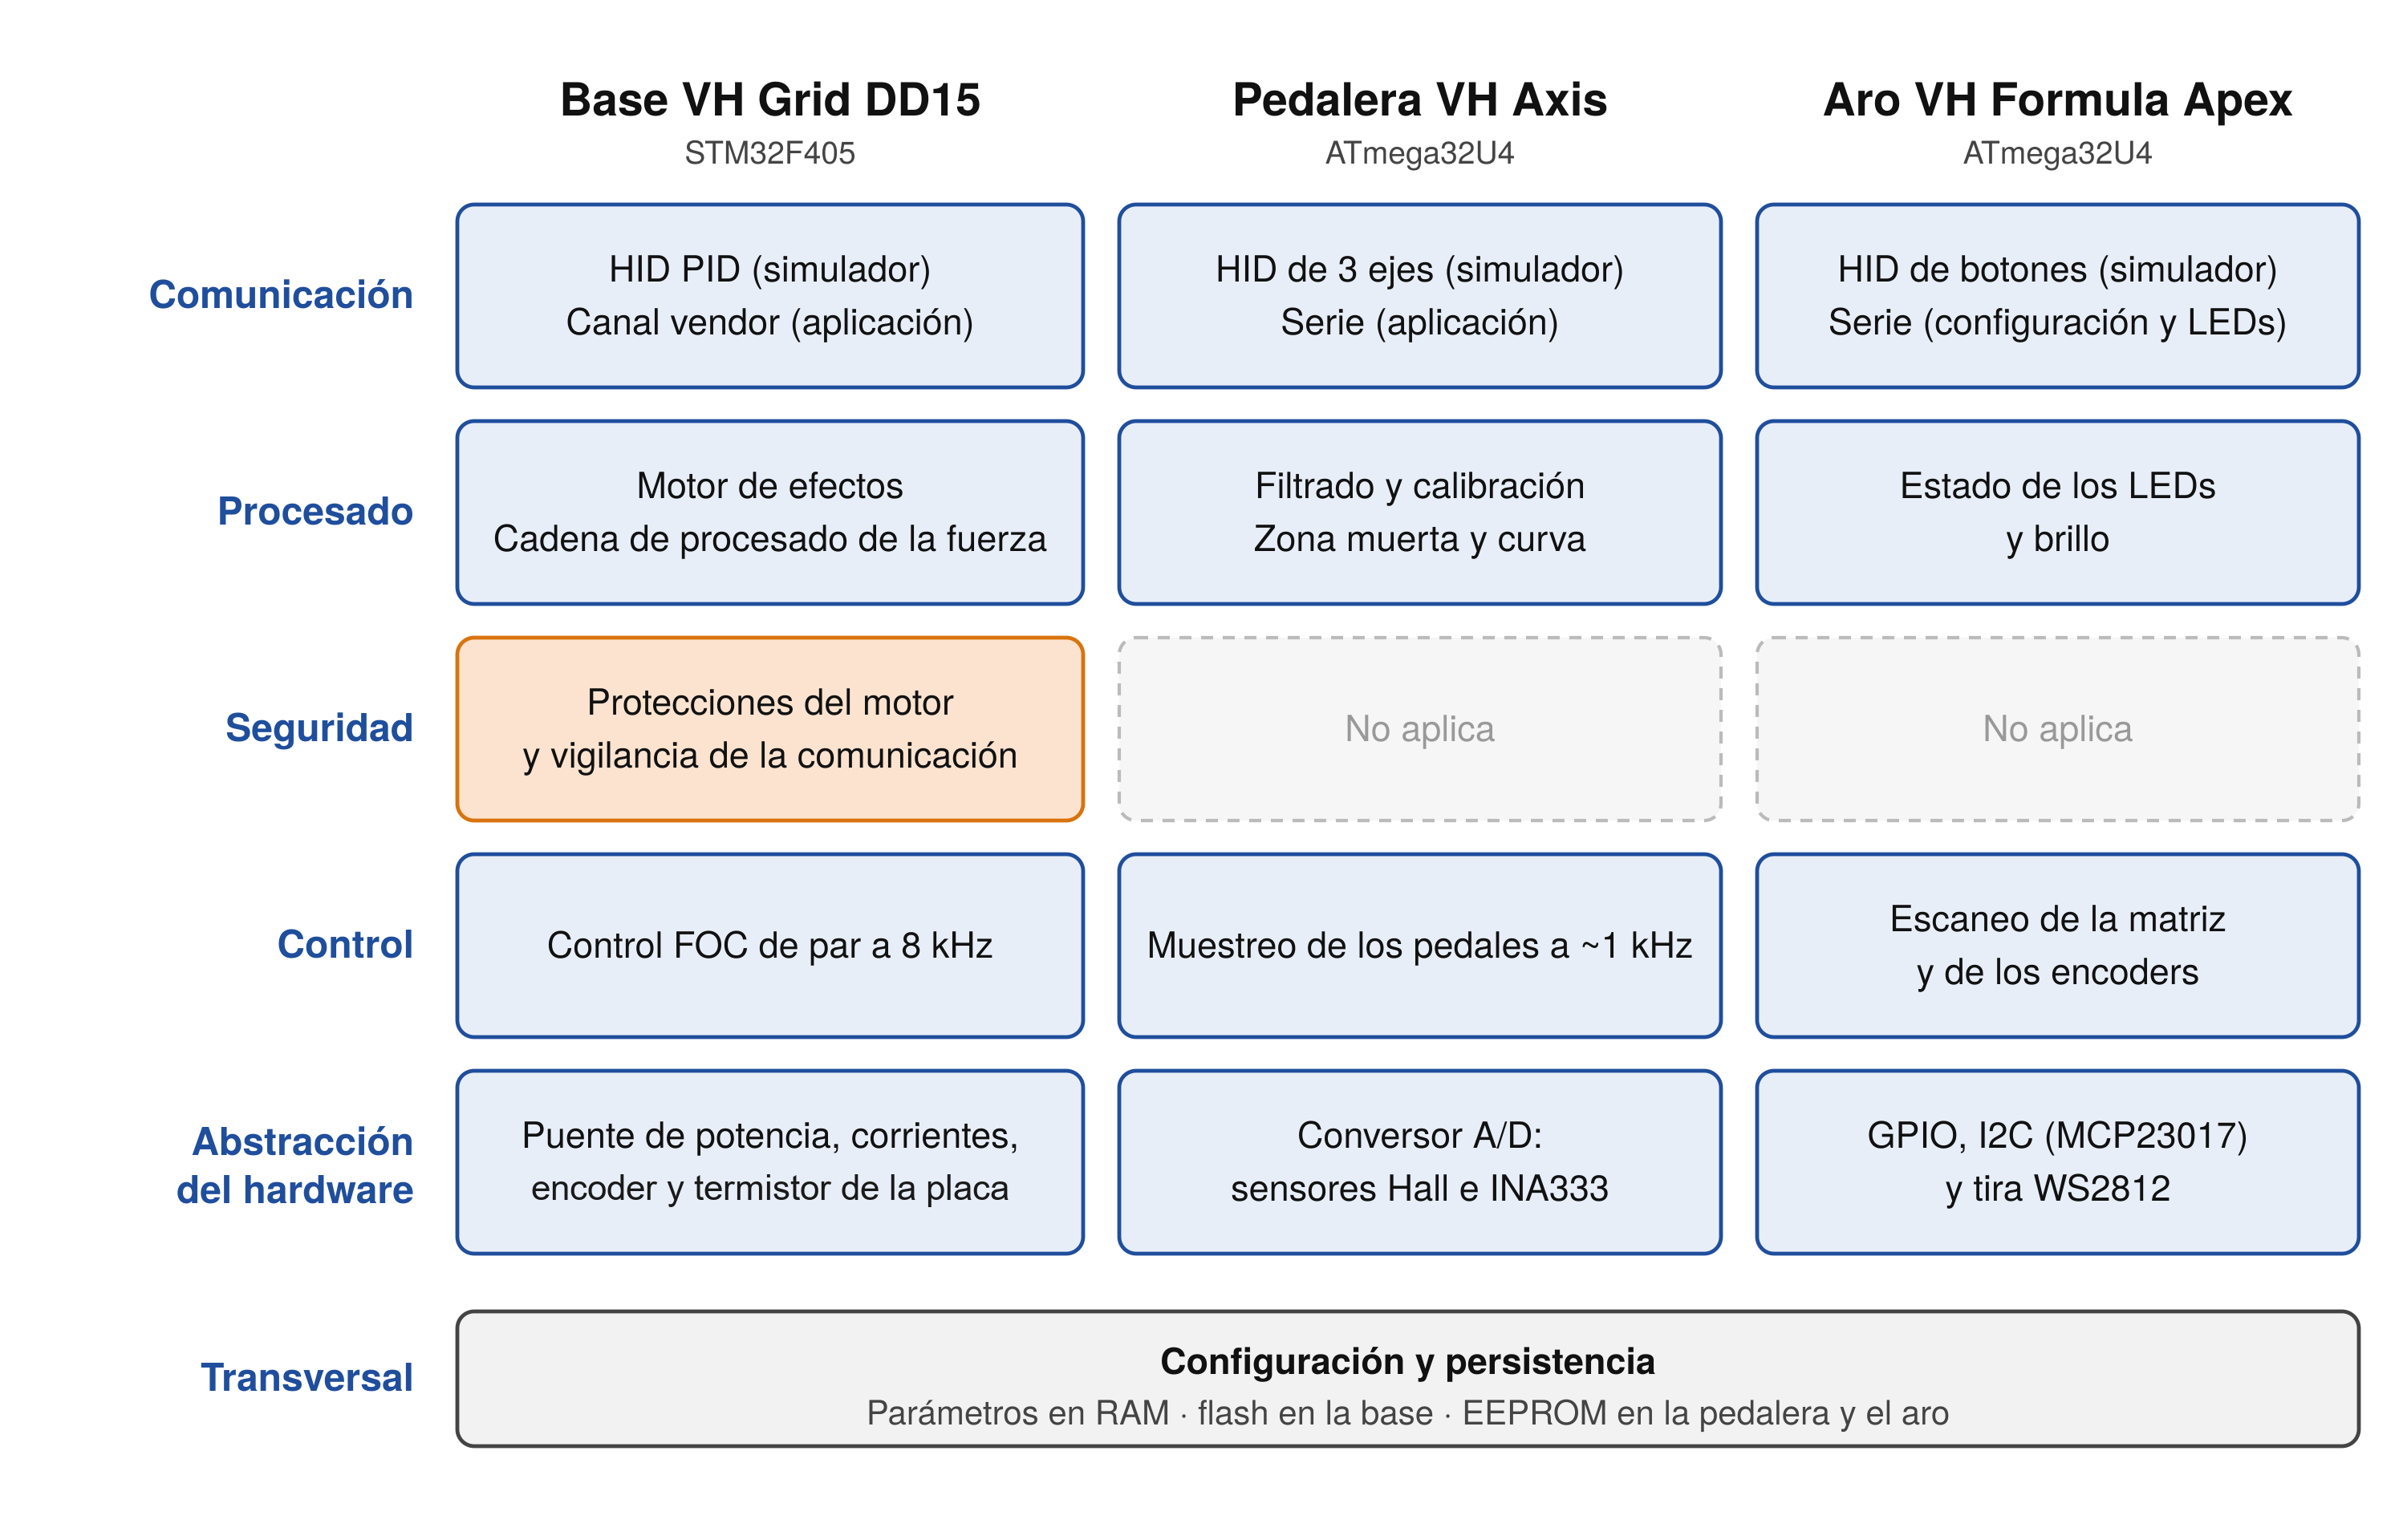
\includegraphics[width=\textwidth]{img/capas-firmware.png}
	\caption{Arquitectura en capas del firmware de los tres periféricos. (Fuente propia)}
	\label{fig:capas-firmware}
\end{figure}

\begin{table}[H]
	\centering
	\caption{Capas del firmware y su función.}
	\label{tab:capas-firmware}
	\small
	\begin{tabularx}{\textwidth}{@{}>{\raggedright\arraybackslash}p{3.2cm}X@{}}
		\toprule
		\textbf{Capa} & \textbf{Función} \\
		\midrule
		Comunicación & Presenta el periférico ante el ordenador con dos canales simultáneos: el HID, que usa el simulador, y el de configuración, que usa la aplicación. En la pedalera y el aro son dos interfaces de un dispositivo USB compuesto; en la base, informes distintos dentro de una sola interfaz HID. \\
		Procesado & Transforma las lecturas o las órdenes recibidas según los ajustes del usuario: el motor de efectos y la cadena de procesado de la fuerza en la base, el filtrado, la calibración y las curvas en la pedalera, y el estado y el brillo de los LEDs en el aro. \\
		Seguridad & Solo en la base. Vigila el estado del motor y de la comunicación, y limita o anula el par ante cualquier anomalía. \\
		Control & Ejecuta el lazo de tiempo real de cada periférico a una frecuencia fija: el control FOC del motor, el muestreo de los pedales o el escaneo de los mandos. \\
		Abstracción del hardware & Encapsula los periféricos del microcontrolador (conversor A/D, temporizadores, PWM, GPIO, I2C y USB) y los sensores y actuadores conectados a ellos. \\
		Configuración y persistencia & Capa transversal. Mantiene los parámetros activos en RAM, los expone a la capa de comunicación para su lectura y modificación en vivo y los guarda en memoria no volátil. \\
		\bottomrule
	\end{tabularx}
\end{table}

\paragraph{Separación entre el juego y la configuración.}
Cada periférico ofrece un canal HID estándar para el simulador y otro independiente para la aplicación. En la pedalera y el aro son dos interfaces de un dispositivo USB compuesto, HID y puerto serie. En la base, que tiene una sola interfaz HID, el canal de configuración es un informe \textit{vendor} propio, separado de los informes PID. Gracias a esta separación, la aplicación puede leer y cambiar ajustes mientras el juego está en marcha sin interferir con los informes de entrada ni con las órdenes de fuerza (RF30), y el periférico funciona como un mando normal aunque la interfaz de configuración no se use nunca (RNF20).

\paragraph{Parámetros en RAM y escritura bajo demanda.}
La capa transversal de configuración mantiene una única copia de los parámetros activos en RAM, que es la que leen las capas de procesado y control. Un cambio llegado desde la aplicación se aplica sobre esa copia y tiene efecto inmediato (RNF5). La escritura en memoria no volátil se hace aparte y solo cuando un valor ha cambiado, para no agotar los ciclos de escritura de la flash y la EEPROM (RNF22). Al arrancar, el periférico carga esa copia guardada, de modo que conserva su configuración aunque se conecte a otro ordenador (RNF19). El contenido exacto de lo que se guarda se describe en la sección~\ref{sec:persistencia}.

\paragraph{Base VH Grid DD15.}
La base es el periférico con la escritura más exigente porque debe atender a la vez tres tipos de trabajo con plazos muy distintos. El \textbf{lazo de control} se ejecuta a 8~kHz con la máxima prioridad: lee la corriente y la posición del motor y calcula la tensión de cada fase mediante el control FOC. Ninguna otra tarea puede retrasarlo, porque un retraso lo notaría el piloto y podría comprometer su seguridad. La \textbf{tarea de fuerza} se ejecuta cada milisegundo (RNF1): recoge los informes recibidos por USB, calcula la fuerza, aplica las protecciones y deja la corriente pedida a disposición del lazo de control. Por último, las \textbf{operaciones puntuales}, como ejecutar la calibración anti-cogging o guardar la configuración en flash, se resuelven dentro de esa misma tarea. Guardar pasa el motor a reposo durante un instante, porque la escritura en flash congela el procesador, y por eso la aplicación agrupa los cambios en lugar de guardar cada uno.

La fuerza que pide el simulador atraviesa una cadena de etapas antes de llegar al motor, representada en la figura~\ref{fig:cadena-fuerza}. El motor de efectos calcula la fuerza de cada efecto activo, e interpola y suaviza la fuerza constante para eliminar los escalones entre informes (RF2). Los efectos que dependen del movimiento (amortiguación, fricción e inercia) y la amortiguación base propia del volante (RF5) siguen un canal aparte, porque cualquier retardo en ellos puede provocar oscilaciones. El resto pasa por el ecualizador de seis bandas (RF6) y por la curva de respuesta de nueve puntos, con su exponente y su fuerza mínima (RF7), y se escala con la fuerza máxima elegida por el usuario (RF4). Por último se suman los dos canales y la fuerza del tope de giro, que tiene su propio límite para mantenerse firme con cualquier fuerza de juego (RF3). Todo este procesado se ejecuta en el propio firmware, lo que mantiene la latencia por debajo de los 2~ms que exige el requisito RNF2.

\begin{figure}[H]
	\centering
	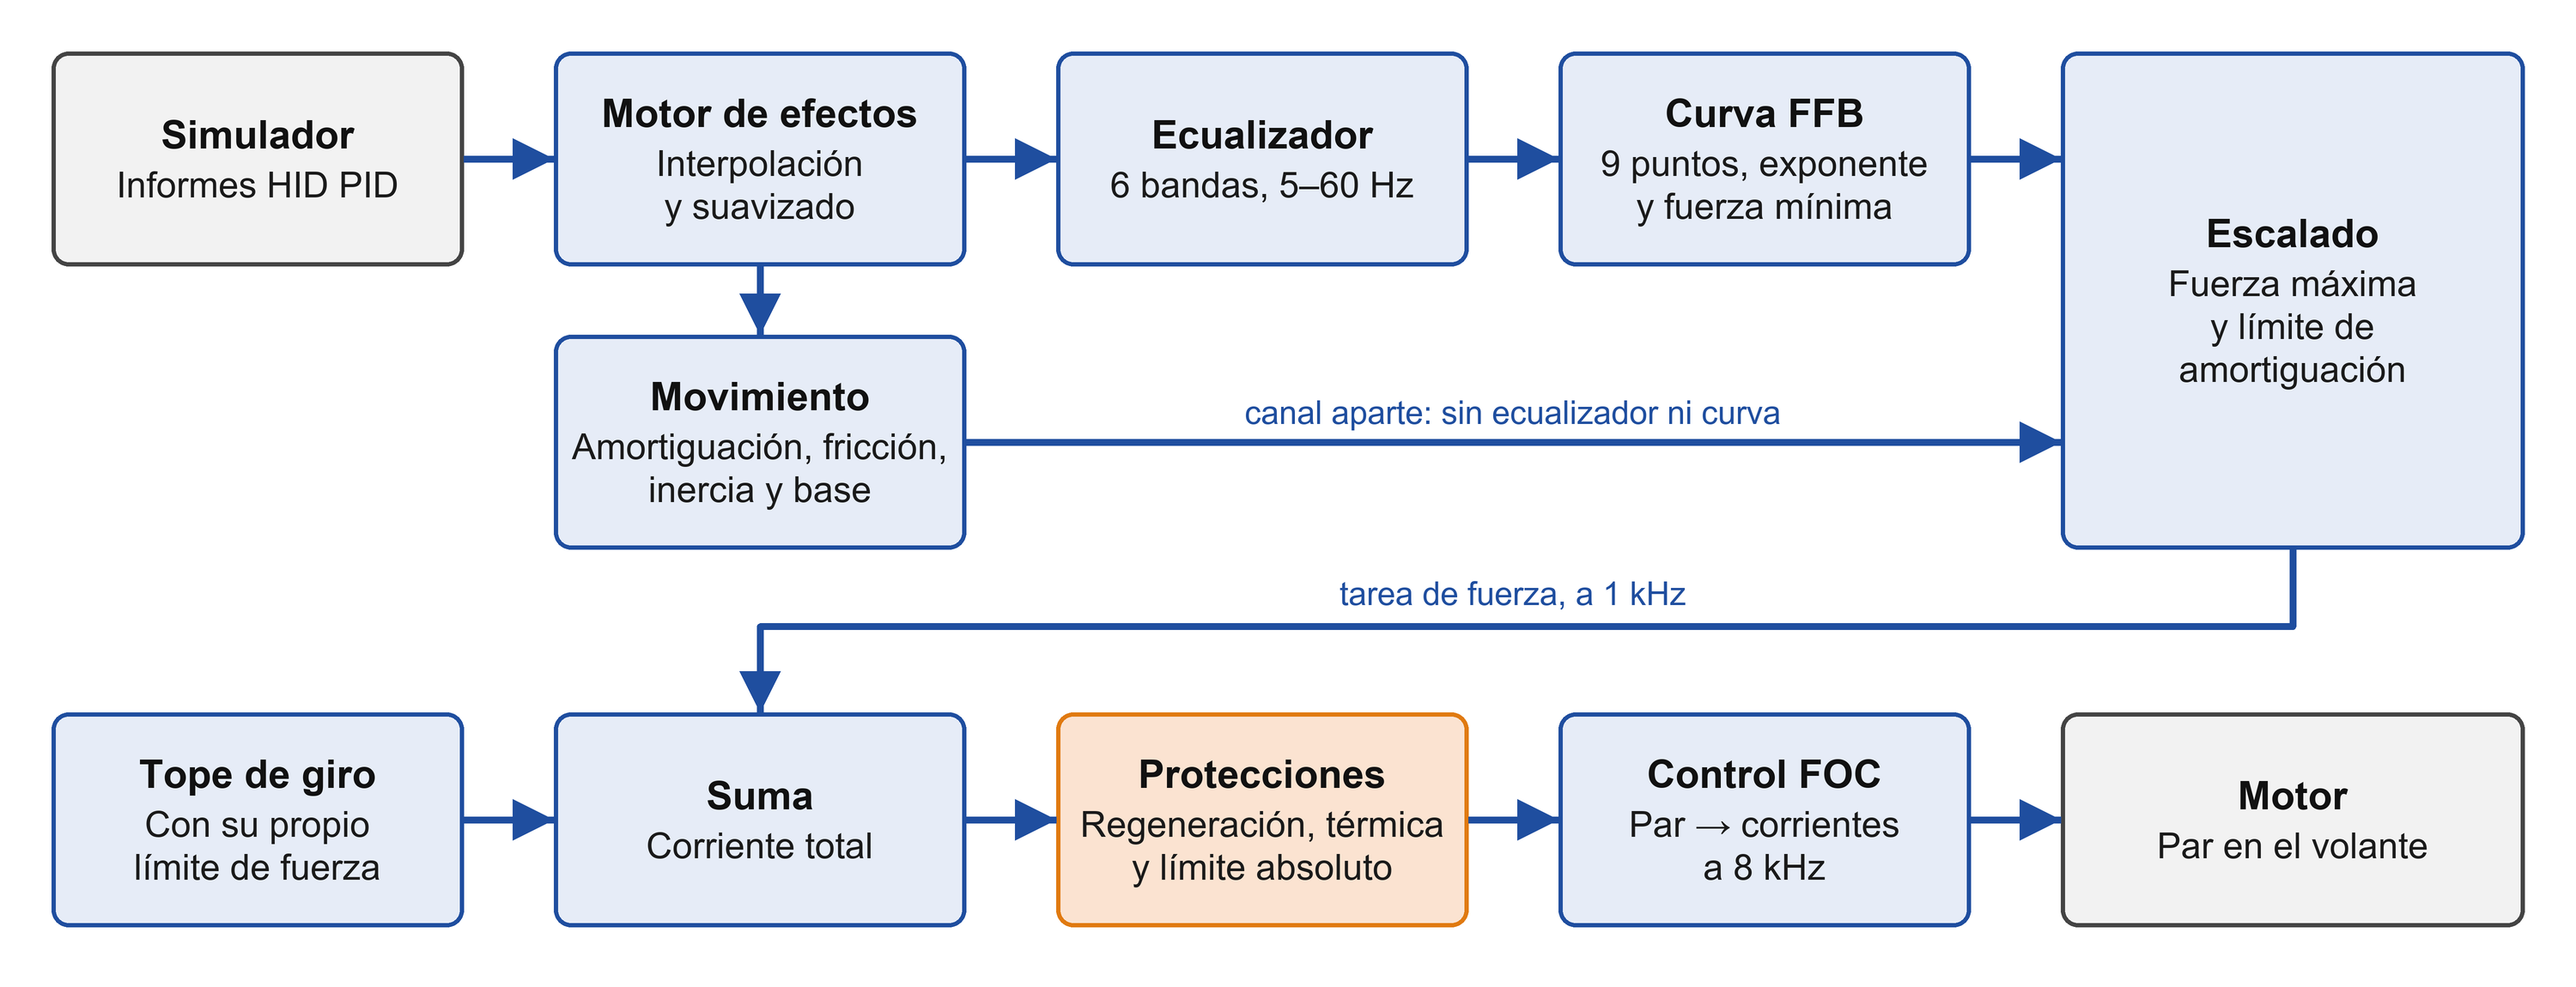
\includegraphics[width=\textwidth]{img/cadena-fuerza.png}
	\caption{Cadena de procesado de la fuerza en la base VH Grid DD15. (Fuente propia)}
	\label{fig:cadena-fuerza}
\end{figure}

Las protecciones que limitan la corriente (regeneración, térmica y límite absoluto) se sitúan al final de la cadena, justo antes del control del motor. Esta posición es una decisión deliberada: al aplicarse sobre la corriente total, sea cual sea el origen de la fuerza, ningún ajuste puede saltarse el sistema de seguridad. La vigilancia de la comunicación y el detector de oscilaciones actúan antes, sobre la fuerza que se está calculando, mientras que la sobrevelocidad y el arranque seguro gobiernan el estado del motor y cortan el par por completo. La tabla~\ref{tab:protecciones} relaciona cada protección con la magnitud que vigila y el requisito al que responde. Su funcionamiento se detalla en el apartado~\ref{subsec:fw-base}.

\begin{table}[H]
	\centering
	\caption{Protecciones de la base VH Grid DD15.}
	\label{tab:protecciones}
	\small
	\begin{tabularx}{\textwidth}{@{}>{\raggedright\arraybackslash}p{3.4cm}>{\raggedright\arraybackslash}X>{\raggedright\arraybackslash}p{1.8cm}@{}}
		\toprule
		\textbf{Protección} & \textbf{Magnitud vigilada y respuesta} & \textbf{Requisito} \\
		\midrule
		Sobrevelocidad & Velocidad del volante medida por el encoder. Limita o corta el par si supera el umbral, por ejemplo al soltar el volante con fuerza aplicada. & RNF8 \\
		Protección térmica & Calentamiento del motor, estimado a partir de la corriente acumulada (modelo I$^2$t), que reduce el par de forma progresiva. Temperatura de los transistores (termistor NTC), que reduce la corriente entre 100 y 120~\textdegree C hasta anularla. & RNF9 \\
		Tope de giro progresivo & Posición del volante respecto al rango configurado. Aplica una fuerza creciente que detiene el volante sin golpe. & RNF10 \\
		Limitador de regeneración & Tensión del bus de alimentación cuando el motor actúa como generador. Limita la energía devuelta a la fuente. & RNF11 \\
		Detector de oscilaciones & Patrón de la velocidad y la posición del volante. Amortigua o corta el par ante oscilaciones sostenidas. & RNF12 \\
		Vigilancia de la comunicación & Tiempo desde el último informe de fuerza. Lleva el par a cero si se pierde la comunicación o el juego deja de enviar fuerzas. & RNF13 \\
		Arranque seguro & Estado del motor y del encoder al encender. No aplica par hasta comprobarlos, y después lo aplica de forma gradual. & RNF14 \\
		\bottomrule
	\end{tabularx}
\end{table}

La base incorpora además una orden de mantenimiento, recibida por el canal \textit{vendor}, que la reinicia en modo de actualización. Esto permite grabar un firmware nuevo desde la aplicación sin manipular la placa (RF32), como se describe en el apartado~\ref{subsec:ux-firmware}.

\paragraph{Pedalera VH Axis y aro VH Formula Apex.}
La pedalera y el aro tienen tareas mucho más sencillas, que no justifican un sistema operativo. Su firmware se organiza como un bucle principal, con cada tarea temporizada a su propio periodo, que recorre las capas en orden, primero lee las entradas, las procesa, actualiza los informes HID y por último atiende los mensajes del puerto serie.

En la pedalera, cada vuelta del bucle lee los tres sensores a unos 1000~Hz (RNF3) y los somete a la misma secuencia que consiste en el filtrado del ruido, normalización entre los puntos de reposo y fondo de la calibración, zona muerta y curva de respuesta (RF12 y RF13). El sentido del pedal se deduce de cuál de sus dos puntos de calibración es mayor, de modo que la calibración guiada resuelve sola un sensor montado al revés, y la aplicación ofrece además una casilla que intercambia ambos puntos. El valor resultante se envía como eje del mando HID. Como toda la transformación se hace en el firmware, la pedalera entrega al simulador la respuesta configurada aunque la aplicación esté cerrada.

En el aro, el bucle escanea la matriz de pulsadores y lee los \textit{encoders} a través del expansor, y envía su estado como botones del mando HID (RF16). Los LEDs siguen un reparto de responsabilidades distinto: la decisión de qué debe mostrar cada LED depende de la telemetría y de los perfiles de luces, que solo conoce la aplicación, por lo que es esta quien calcula el estado de la tira y lo envía por el puerto serie. El aro se limita a aplicarlo con el brillo configurado, que guarda en su EEPROM para conservarlo aunque arranque sin el ordenador (RF21). Al conectarse, aro y aplicación intercambian un saludo (\textit{handshake}) que identifica al periférico y su versión de firmware antes de empezar a enviar datos.

\subsection{Aplicación}
\label{subsec:arq-aplicacion}
La aplicación VH SimGrid se desarrolla en Python para Windows 10 y 11 (RNF40). Las primeras versiones se construyeron con \textbf{Tkinter}, la biblioteca gráfica que se incluye de serie con Python. Es sencilla y no necesita instalar nada, por lo que resultó adecuada para los primeros prototipos, que solo leían y cambiaban los ajustes de los periféricos. Sin embargo, cuando la aplicación creció y pasó a incluir el \textit{dash}, las gráficas del análisis y una interfaz más cuidada, sus limitaciones en rendimiento gráfico, personalización visual y trabajo con varios hilos hicieron necesario cambiar de tecnología.

Se decidió migrar a \textbf{Qt}, un \textit{framework} de aplicaciones de escritorio mucho más completo. Frente a Tkinter, ofrece una escena gráfica que solo redibuja lo que cambia, para mantener el \textit{dash} a 30 imágenes por segundo sin sobrecargar el equipo (RNF6 y RNF7), hojas de estilo para los modos claro y oscuro, señales seguras entre hilos y soporte de varias pantallas para la pantalla del aro (RF22). La traducción de la interfaz (RNF27) se resuelve con un módulo propio, con un diccionario por idioma. A cambio, aumenta el tamaño del instalador y es más complejo de aprender, dos costes que se consideraron asumibles. La tabla~\ref{tab:tkinter-qt} resume la comparación.

\begin{table}[H]
	\centering
	\caption{Comparación entre Tkinter y Qt.}
	\label{tab:tkinter-qt}
	\small
	\begin{tabularx}{\textwidth}{@{}>{\raggedright\arraybackslash}p{3.4cm}>{\raggedright\arraybackslash}X>{\raggedright\arraybackslash}X@{}}
		\toprule
		\textbf{Criterio} & \textbf{Tkinter} & \textbf{Qt} \\
		\midrule
		Instalación y aprendizaje & Incluido en Python y muy sencillo. & Biblioteca externa y más compleja. \\
		Rendimiento gráfico & Lienzo básico. & Escena gráfica que solo redibuja lo que cambia. \\
		Personalización visual & Limitada. & Hojas de estilo para toda la aplicación. \\
		Trabajo con hilos & Sin mecanismo propio. & Señales y ranuras seguras entre hilos. \\
		Varias pantallas & Solución propia. & Soporte integrado. \\
		\bottomrule
	\end{tabularx}
\end{table}

La aplicación se organiza en tres capas: la \textbf{interfaz}, con la que interactúa el usuario; la \textbf{lógica}, que contiene toda la funcionalidad del sistema, y la \textbf{persistencia}, que guarda los datos en el disco. La figura~\ref{fig:arquitectura-app} muestra esta organización.

\begin{figure}[H]
	\centering
	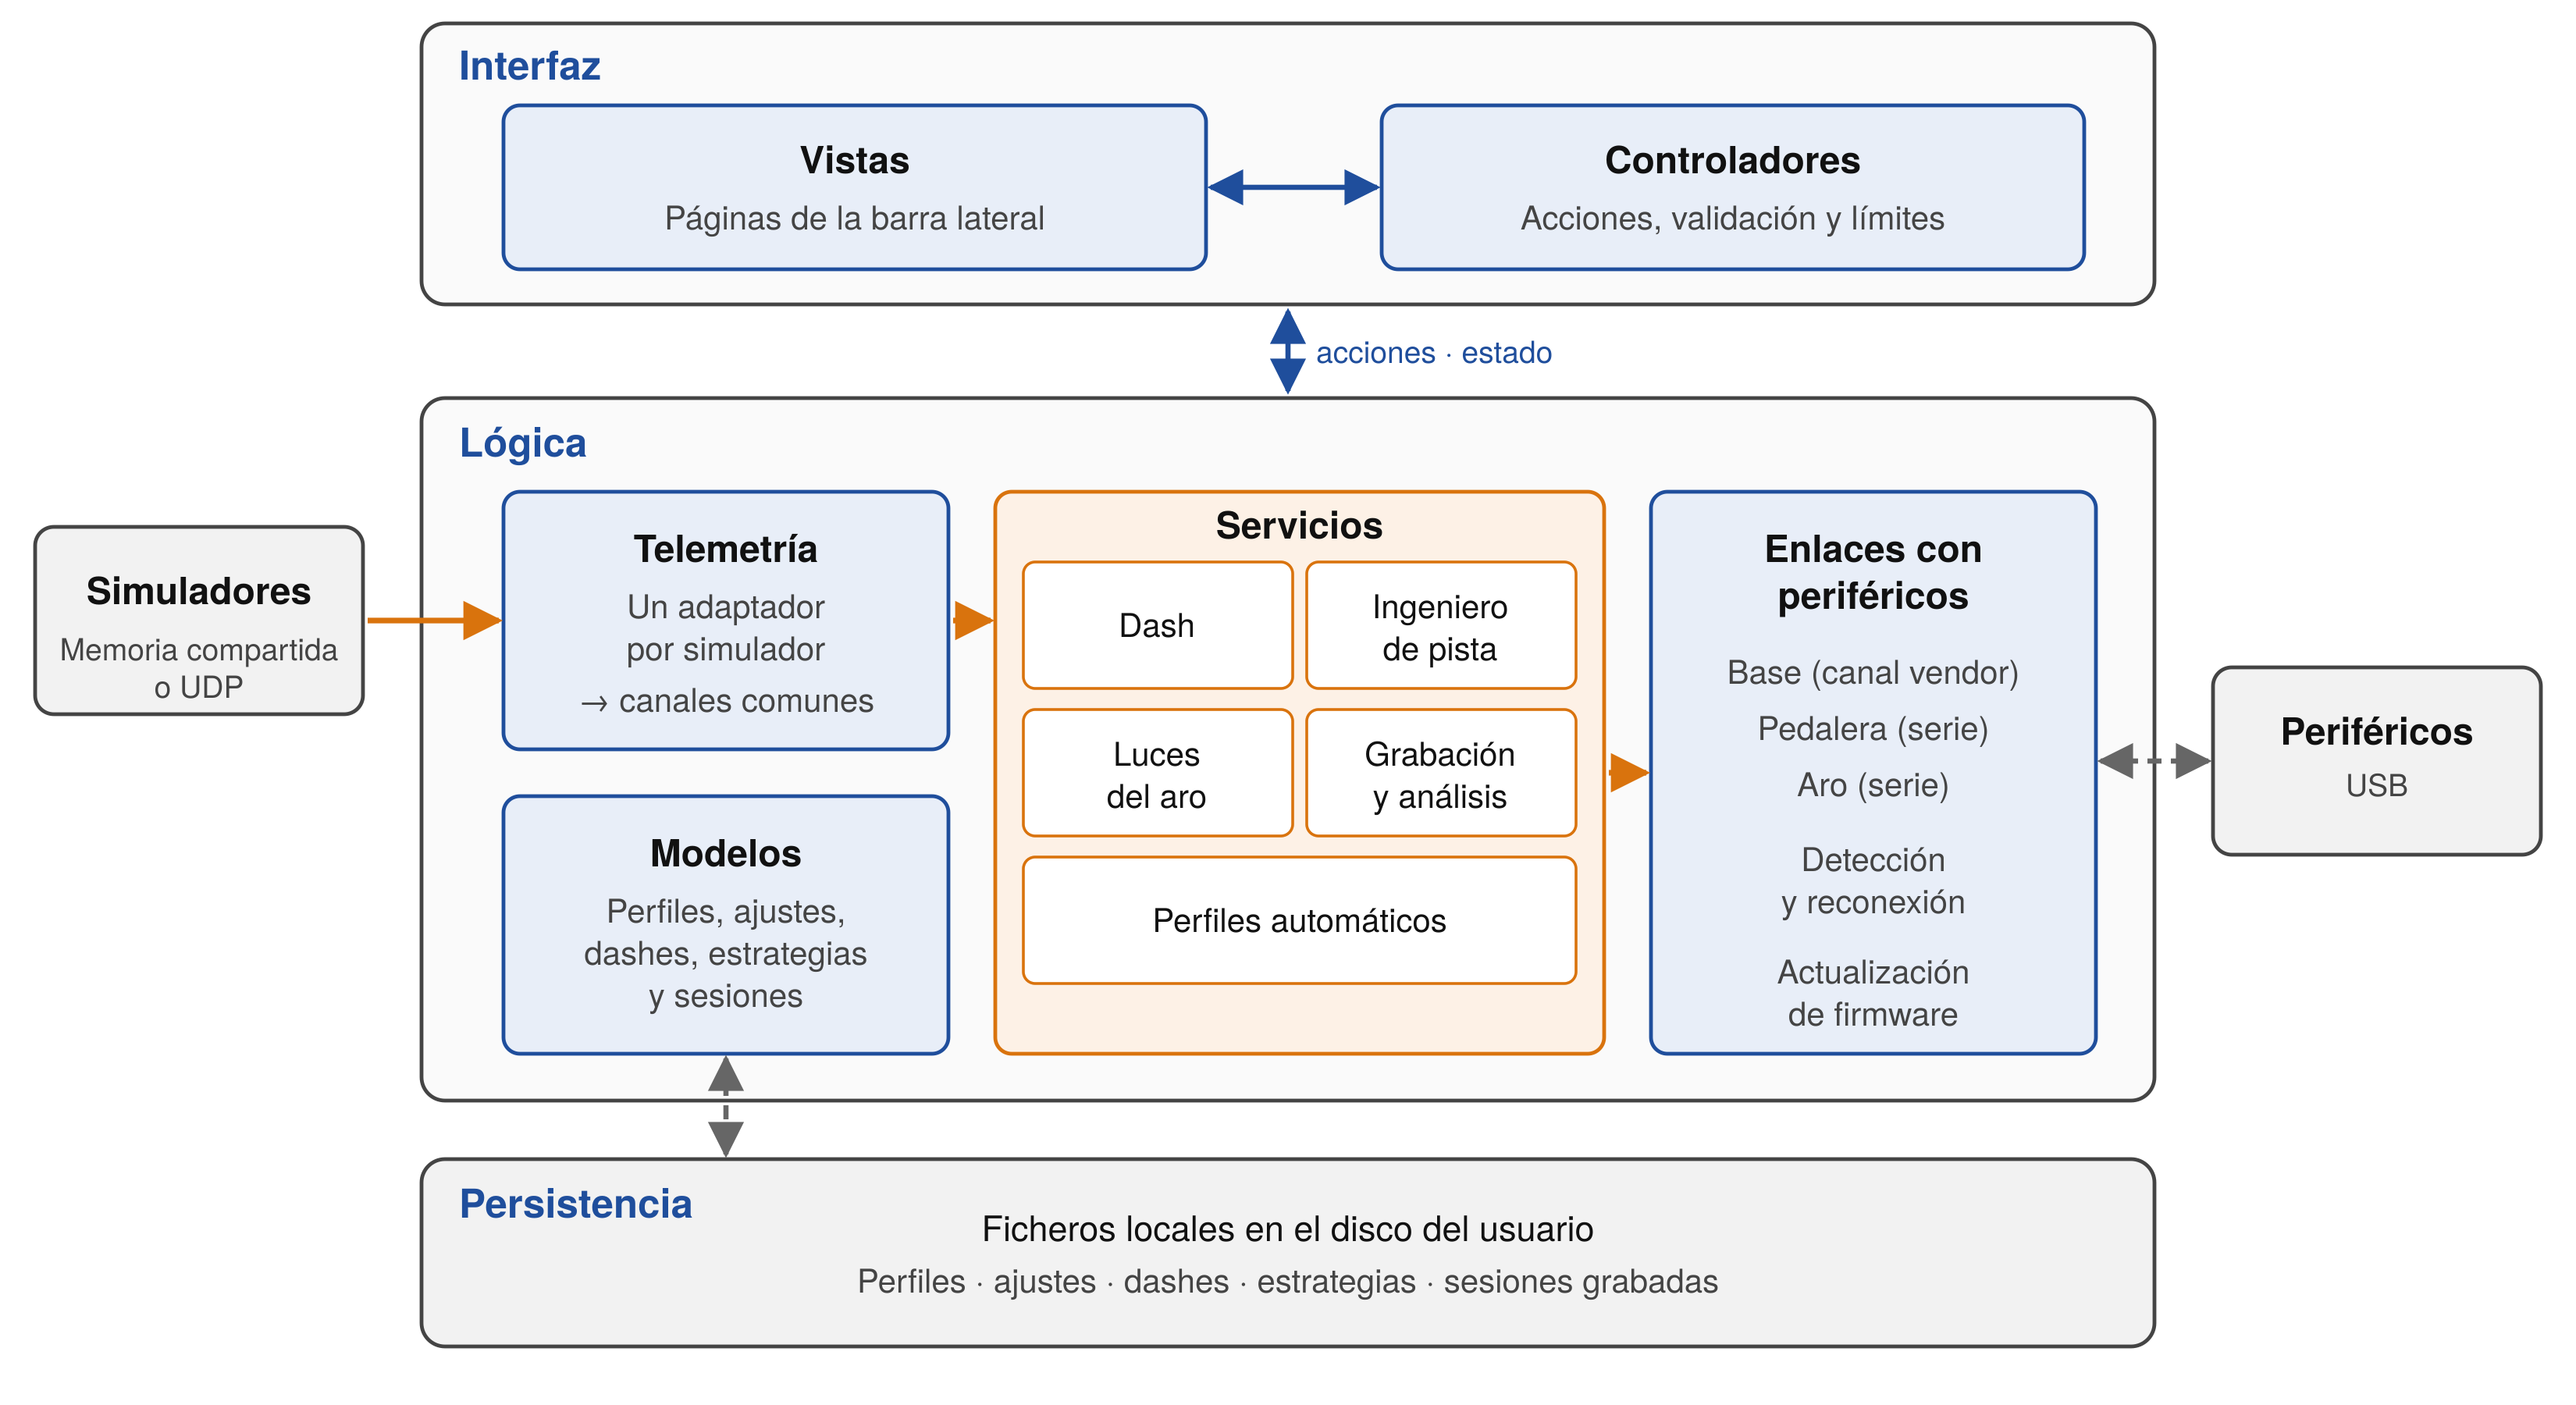
\includegraphics[width=\textwidth]{img/arquitectura-app.png}
	\caption{Arquitectura de la aplicación VH SimGrid. (Fuente propia)}
	\label{fig:arquitectura-app}
\end{figure}

\paragraph{Interfaz: vistas y controladores.}
La capa de interfaz separa lo que se muestra de lo que se hace. Las \textbf{vistas} son las páginas de la aplicación (Inicio, Volante, Aro, Pedalera, Dash, Ingeniero, Análisis y Ajustes) y solo se ocupan de presentar datos y recoger las acciones del usuario. Los \textbf{controladores} reciben esas acciones, comprueban que los valores están dentro de los límites permitidos (RNF39) y las trasladan a la capa de lógica. Las vistas nunca se comunican directamente con los periféricos ni con los simuladores, de modo que el aspecto de una página puede cambiar sin afectar al funcionamiento del sistema.

\paragraph{Lógica.}
La capa de lógica se divide en cuatro bloques:

\begin{itemize}
	\item \textbf{Modelos.} Representan en memoria los datos del sistema: los perfiles, los ajustes de cada periférico, los \textit{dashes}, las estrategias y las sesiones. Son independientes de cómo se muestran en la interfaz y de cómo se guardan en el disco.
	\item \textbf{Enlaces con periféricos.} Cada periférico tiene su propio enlace, que encapsula su protocolo: el canal \textit{vendor} de la base y el puerto serie de la pedalera y el aro. Los enlaces detectan los periféricos por su identidad USB al conectarlos y los reconectan si se pierde la conexión (RF29). Incluyen también el actualizador de firmware, que elige el fichero según el periférico conectado y comprueba la grabación al terminar (RF32 y RNF15).
	\item \textbf{Telemetría.} Cada simulador publica sus datos con su propio formato y por su propio medio, ya sea memoria compartida o paquetes UDP. Para aislar al resto de la aplicación de esta diversidad, cada simulador tiene su \textbf{adaptador}, que traduce sus datos a un conjunto común de canales (velocidad, marcha, revoluciones, posición en pista\ldots) y calcula los canales derivados que el juego no ofrece. Añadir un simulador consiste en escribir un adaptador nuevo, sin modificar nada más (RF38 y RNF43).
	\item \textbf{Servicios.} Son las funciones que consumen los canales comunes de telemetría: el \textit{dash}, que se dibuja en la pantalla del aro o en un monitor y se sirve a los móviles vinculados; el ingeniero de pista, con su motor de reglas, la síntesis de voz (Piper) y el reconocimiento de voz (Vosk); las luces del aro, que calculan el estado de la tira y lo envían por su enlace; la grabación y el análisis de sesiones, y los perfiles automáticos, que detectan el juego y el coche y aplican el perfil correspondiente. La voz y las grabaciones se procesan y guardan siempre en el propio equipo (RNF42).
\end{itemize}

Como todos los servicios trabajan sobre los mismos canales comunes, ninguno depende del simulador concreto. El mismo \textit{dash}, la misma lógica del ingeniero y las mismas hojas de análisis sirven para los 18 juegos compatibles.

\paragraph{Ejecución concurrente.}
La interfaz se ejecuta en el hilo principal, mientras que la recepción de la telemetría, los enlaces con los periféricos y el procesado de voz se ejecutan en hilos propios, que se comunican con el resto mediante colas y, en algunos casos, señales de Qt. Así, una operación lenta, como cargar una sesión grabada o reconocer una frase, nunca bloquea la interfaz, y las luces del aro se actualizan al ritmo de la telemetría con independencia de lo que se esté dibujando en pantalla (RNF4). Esta organización permite también mantener acotado el consumo de procesador mientras el simulador está en marcha (RNF7).

\paragraph{Ejemplo de funcionamiento.}
El recorrido de un cambio de ajuste muestra cómo colaboran las capas. Cuando el usuario mueve el control de la fuerza máxima en la página del volante, la vista notifica la acción a su controlador, que comprueba que el valor está dentro de los límites y actualiza el modelo del perfil activo. El enlace de la base envía el nuevo valor por el canal \textit{vendor}, y el firmware lo aplica en la copia de parámetros en RAM, con efecto inmediato. Cinco segundos después del último cambio, la aplicación le pide que lo guarde en flash. El perfil del disco solo cambia cuando el usuario lo guarda. Todo el recorrido, desde que el usuario suelta el control hasta que el motor aplica la nueva fuerza, debe completarse en menos de 200~ms (RNF5).

\section{Protocolos de comunicación}
\label{sec:protocolos}
Los protocolos de comunicación son el contrato entre las partes del sistema, es decir, fijan cómo se identifica el periférico, qué mensajes intercambia con el simulador y con la aplicación y, además, cómo se comunica la aplicación con un dispositivo móvil para reproducir el \textit{dash}.

Todos los periféricos siguen el mismo patrón, ya presentado en la sección~\ref{sec:arquitectura-tecnologica}, cada uno ofrece dos canales, uno HID estándar para el simulador y otro de configuración para la aplicación. La primera sigue especificaciones públicas y no se modifica; la segunda es propia del proyecto y es la que se describe con más detalle. Además, todas las comunicaciones de configuración siguen la misma secuencia al conectar un periférico, representada en la figura~\ref{fig:secuencia-conexion}:

\begin{enumerate}
	\item Al enchufarlo, el periférico se identifica ante Windows con su identidad USB y su nombre, y el sistema avisa a la aplicación.
	\item La aplicación le pide su modelo y su versión de firmware, y si hay una versión más reciente ofrece actualizarlo (RF32).
	\item La aplicación lee la configuración guardada en la base o en la pedalera, de modo que la interfaz muestra siempre los valores reales del dispositivo, y no una copia que podría estar desactualizada. El aro solo guarda el brillo, que le envía la aplicación.
	\item Mientras está conectado, la aplicación envía los cambios de ajuste y recibe el estado en vivo del periférico.
\end{enumerate}

\begin{figure}[H]
	\centering
	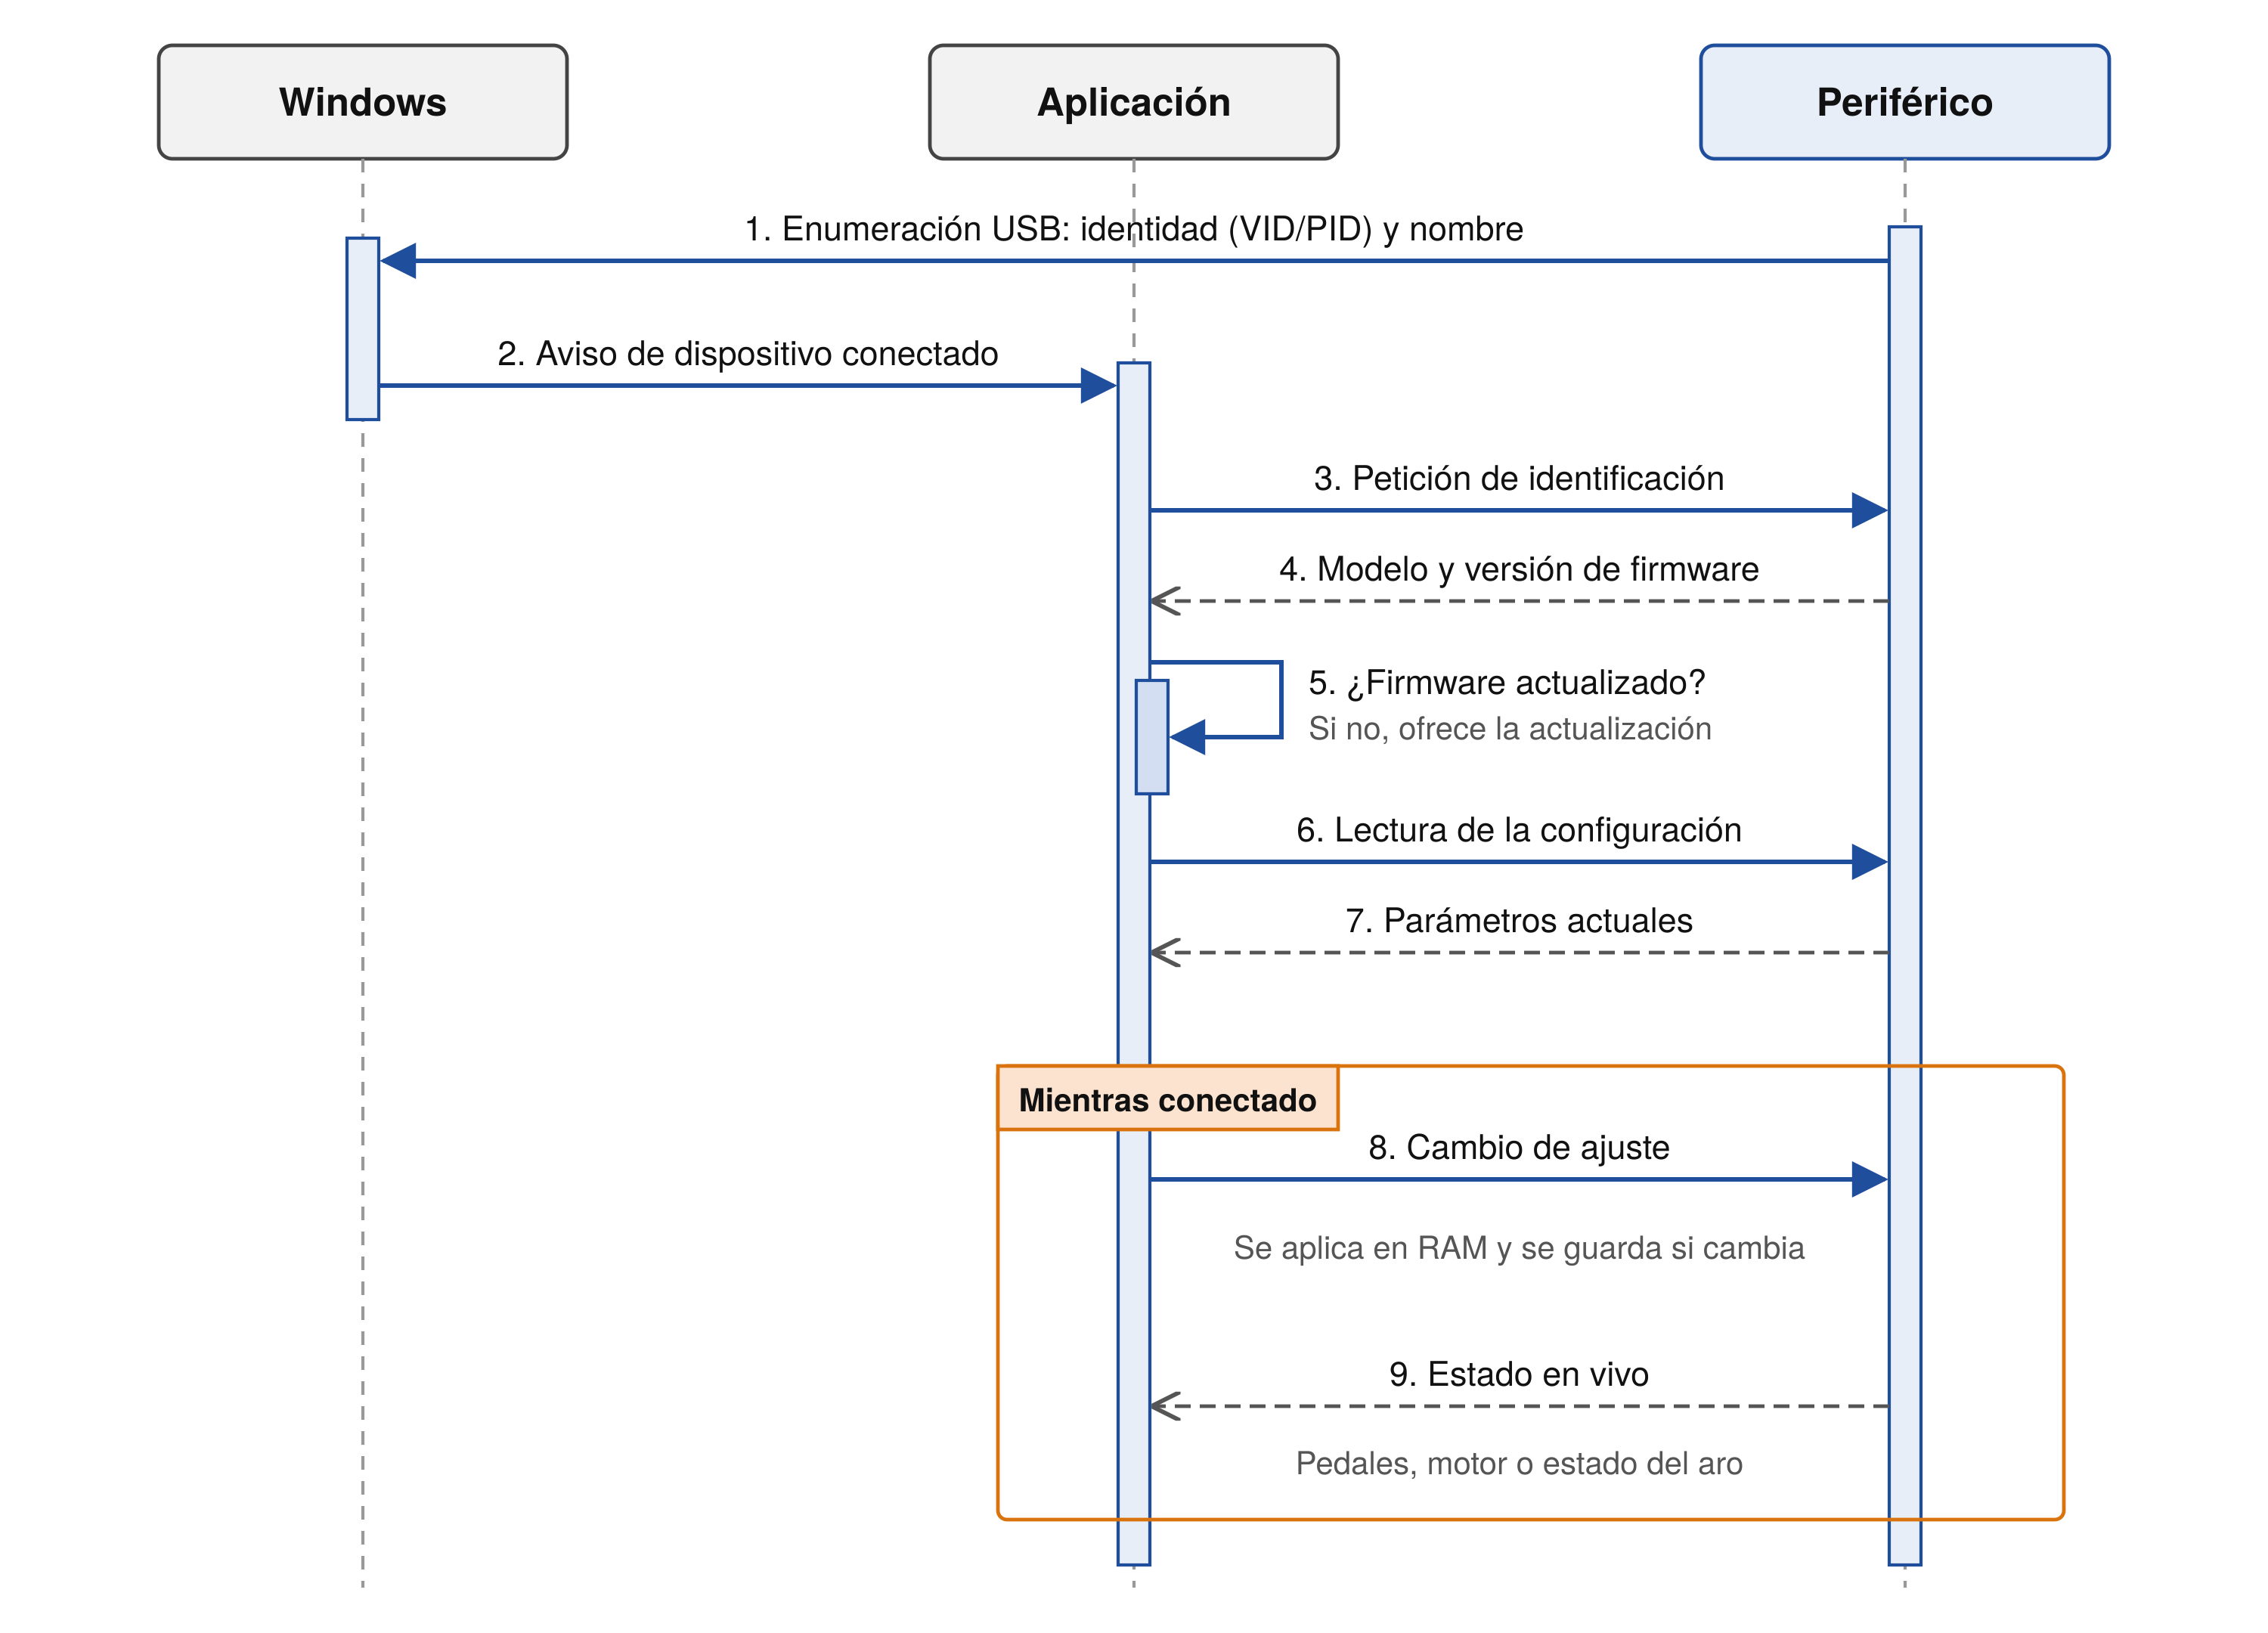
\includegraphics[width=0.9\textwidth]{img/secuencia-conexion.png}
	\caption{Secuencia de conexión entre la aplicación y un periférico. (Fuente propia)}
	\label{fig:secuencia-conexion}
\end{figure}

Leer la configuración del periférico, en lugar de imponerle la de la aplicación, es una decisión de diseño coherente con la filosofía de no depender de la aplicación para utilizar los periféricos. Solo si la base ha perdido sus ajustes, la aplicación se los devuelve a partir de la última copia que guardó.

\subsection{Identidad USB}
\label{subsec:identidad-usb}
Todo dispositivo USB se identifica con dos números de 16 bits: el identificador del fabricante (VID, \textit{Vendor ID}) y el del producto (PID, \textit{Product ID}). Junto a ellos, el dispositivo declara su nombre de producto, que es el que Windows muestra en su panel de dispositivos de juego y el que ven los simuladores al asignar los mandos.

Cada periférico tiene una identidad propia, recogida en la tabla~\ref{tab:identidad-usb}. Esta identidad cumple dos funciones. Para el usuario, los periféricos aparecen con su nombre en Windows y en los juegos, y no con un nombre genérico de la placa. Para la aplicación, es lo que permite la detección automática (RF29): al conectarse un dispositivo, la aplicación compara su VID y su PID con los de los tres periféricos y solo abre la comunicación con los que reconoce, sin confundirlos con otros mandos o placas conectados al mismo ordenador. La identidad permite además saber qué firmware corresponde a cada dispositivo antes de grabarlo (RNF15).

\begin{table}[H]
	\centering
	\caption{Identidad USB de los periféricos.}
	\label{tab:identidad-usb}
	\small
	\begin{tabularx}{\textwidth}{@{}>{\raggedright\arraybackslash}p{1.6cm}>{\raggedright\arraybackslash}p{2.8cm}>{\raggedright\arraybackslash}p{2.8cm}>{\raggedright\arraybackslash}X@{}}
		\toprule
		\textbf{Periférico} & \textbf{VID:PID} & \textbf{Nombre en Windows} & \textbf{Interfaces} \\
		\midrule
		Base & \texttt{0x1209:0xFFB1} & VH Grid DD15 & HID PID (volante con \textit{force feedback}) y canal \textit{vendor} de configuración. \\
		Pedalera & \texttt{0x2341:0x8037} & VH Axis & HID (mando de tres ejes) y puerto serie de configuración. \\
		Aro & \texttt{0x2341:0x8055} & VH Formula Apex & HID (mando de botones) y puerto serie de configuración y LEDs. \\
		\bottomrule
	\end{tabularx}
\end{table}

\subsection{Comunicación con la base}
\label{subsec:protocolo-base}
\paragraph{Interfaz HID PID.}
La comunicación con el simulador sigue la especificación HID PID (\textit{Physical Interface Device}) del USB-IF, la misma que usan los volantes comerciales, y que Windows traduce a la interfaz DirectInput de los juegos (RF1). La especificación define tres tipos de informe, que la base implementa según la tabla~\ref{tab:informes-pid}. El descriptor de la interfaz, que declara a Windows qué informes admite la base, se basa en el del proyecto abierto OpenFFBoard.

\begin{table}[H]
	\centering
	\caption{Tipos de informe HID PID que usa la base.}
	\label{tab:informes-pid}
	\small
	\begin{tabularx}{\textwidth}{@{}>{\raggedright\arraybackslash}p{2.4cm}>{\raggedright\arraybackslash}p{2.6cm}X@{}}
		\toprule
		\textbf{Tipo} & \textbf{Sentido} & \textbf{Contenido} \\
		\midrule
		Entrada & Base a simulador & Posición del volante, que el juego lee como el eje de dirección. \\
		Salida & Simulador a base & Definición y control de los efectos: crear un efecto y fijar sus parámetros (fuerza constante, muelle, amortiguación, fricción, inercia), iniciarlo o detenerlo, la ganancia global y las órdenes generales del dispositivo, como activar o desactivar los actuadores. \\
		Característica & Ambos & Reserva de memoria para un efecto nuevo y respuesta de la base indicando si lo ha podido crear. \\
		\bottomrule
	\end{tabularx}
\end{table}

La base atiende estos informes cada milisegundo (RNF1). Si dejan de llegar, porque se pierde la comunicación o el juego se cierra, la vigilancia de la comunicación lleva el par a cero (RNF13).

\paragraph{Canal \textit{vendor}.}
La configuración de la base viaja por un canal \textit{vendor}, es decir, un informe HID definido por el propio fabricante (identificador \texttt{0xA1}), dentro de la misma interfaz, que Windows no interpreta, de modo que no interfiere con los informes PID que usa el juego. El diseño del canal se basa en un modelo de \textbf{parámetros}, es decir, cada ajuste de la base (fuerza máxima, rango de giro, cada banda del ecualizador, cada punto de la curva\ldots) tiene un identificador numérico, y la aplicación los lee y escribe de uno en uno. Este modelo tiene dos ventajas, por un lado añadir un ajuste nuevo en el firmware solo requiere asignarle un identificador, sin cambiar el formato de los mensajes, y por otro lado, la aplicación puede aplicar cualquier cambio al instante, sin reenviar la configuración completa (RF30 y RNF5). La tabla~\ref{tab:canal-vendor} resume las operaciones del canal.

\begin{table}[H]
	\centering
	\caption{Operaciones del canal \textit{vendor} de la base.}
	\label{tab:canal-vendor}
	\small
	\begin{tabularx}{\textwidth}{@{}>{\raggedright\arraybackslash}p{2.8cm}>{\raggedright\arraybackslash}p{1cm}>{\raggedright\arraybackslash}p{1.6cm}X@{}}
		\toprule
		\textbf{Operación} & \textbf{Tipo} & \textbf{Código} & \textbf{Descripción} \\
		\midrule
		Identificación & \texttt{0x01} & 207 & Devuelve la versión del firmware. \\
		Leer parámetro & \texttt{0x01} & 1--35 & Devuelve el valor actual de un parámetro. \\
		Escribir parámetro & \texttt{0x02} & 1--35 & Cambia el valor de un parámetro en RAM, con efecto inmediato. El firmware ajusta a sus límites los valores que los superan y devuelve el valor aplicado (RNF39). \\
		Centrar & \texttt{0x03} & 100 & Fija la posición actual del volante como centro (RF3). \\
		Calibración anti-cogging & \texttt{0x03} & 106 & Inicia la medida del rizado magnético y guarda el resultado en flash (RF8). \\
		Estado en vivo & \texttt{0x01} & 200--206, 208--215 & Devuelve el estado y los errores del motor, la posición, la tensión de bus, la fuerza pedida, la carga térmica, la temperatura y los contadores de las protecciones, que alimentan la monitorización de la aplicación (RF9). \\
		Reinicio & \texttt{0x03} & 107 & Reinicia la base (RF10). \\
		Modo de actualización & \texttt{0x03} & 105 & Reinicia la base en el modo de grabación de firmware, sin necesidad del puente BOOT0 (RF32). \\
		\bottomrule
	\end{tabularx}
\end{table}

Todos los mensajes del canal tienen el mismo formato en los dos sentidos, recogido en la tabla~\ref{tab:formato-vendor}. Es un informe HID de 25 bytes, con los campos de varios bytes en orden \textit{little-endian}. La base responde a cada petición con el mismo mensaje, en el que marca el campo de tipo y rellena el valor. Si la petición no es válida, como ocurre con un código desconocido, lo indica en ese mismo campo.

\begin{table}[H]
	\centering
	\caption{Formato de los mensajes del canal \textit{vendor}.}
	\label{tab:formato-vendor}
	\small
	\begin{tabularx}{\textwidth}{@{}>{\raggedright\arraybackslash}p{2.8cm}>{\raggedright\arraybackslash}p{1.4cm}X@{}}
		\toprule
		\textbf{Campo} & \textbf{Bytes} & \textbf{Contenido} \\
		\midrule
		ID de informe & 1 & Siempre \texttt{0xA1}. \\
		Tipo & 1 & \texttt{0x01} leer, \texttt{0x02} escribir, \texttt{0x03} acción. La respuesta añade \texttt{0x80} y, si hay error, también \texttt{0x40}. \\
		Clase e instancia & 2 + 1 & Sin uso, a cero. Se conservan del descriptor de OpenFFBoard. \\
		Comando & 4 & Código de la operación o del parámetro. \\
		Valor & 8 & Valor leído o que se quiere escribir. \\
		Dirección & 8 & Sin uso, a cero. \\
		\bottomrule
	\end{tabularx}
\end{table}

\subsection{Comunicación con la pedalera y el aro}
\label{subsec:protocolo-pedalera-aro}
La pedalera y el aro se presentan ante el simulador como mandos HID estándar, la pedalera con tres ejes (RF11) y el aro con sus botones (RF16). Estos informes los define la propia especificación HID, sin ninguna extensión, por lo que cualquier juego los reconoce.

Para la configuración, ambos usan un \textbf{puerto serie virtual} sobre USB, que Windows reconoce como un puerto COM sin necesidad de controladores. Se eligió el puerto serie porque es la forma más sencilla de comunicarse con un ATmega32U4 y porque permite enviar mensajes en ambos sentidos en cualquier momento, lo que la pedalera necesita para la traza en vivo y el aro para recibir el estado de los LEDs. Los dos periféricos comparten el mismo esquema de mensajes, basado en órdenes de la aplicación y respuestas del periférico, y se diferencian en las operaciones que admiten, recogidas en la tabla~\ref{tab:comandos-serie}.

\begin{table}[H]
	\centering
	\caption{Operaciones del canal serie de la pedalera y el aro.}
	\label{tab:comandos-serie}
	\small
	\begin{tabularx}{\textwidth}{@{}>{\raggedright\arraybackslash}p{2.4cm}>{\raggedright\arraybackslash}p{1.5cm}>{\raggedright\arraybackslash}p{3.6cm}X@{}}
		\toprule
		\textbf{Operación} & \textbf{Periférico} & \textbf{Mensaje} & \textbf{Descripción} \\
		\midrule
		Identificación & Ambos & \texttt{VER} (pedalera), \texttt{PING} (aro) & Saludo inicial (\textit{handshake}): el periférico devuelve su modelo y su versión de firmware. \\
		Leer configuración & Pedalera & \texttt{GETCAL} & Devuelve los ajustes activos en una línea \texttt{CALDATA}. \\
		Escribir ajustes & Pedalera & \texttt{CAL,<30 valores>} & Cambia los 30 ajustes a la vez: reposo, fondo, zona muerta y 7 puntos de curva por pedal. Los aplica al momento, guarda en EEPROM solo lo que ha cambiado y responde \texttt{CALOK} o \texttt{CALERR} (RF14 y RNF22). \\
		Calibrar & Pedalera & \texttt{CAL,<30 valores>} & La aplicación toma de la traza la lectura de un pedal como su posición de reposo o de fondo, y la envía con este mensaje (RF12). \\
		Traza en vivo & Pedalera & \texttt{<a>,<e>,<f>} y \texttt{FINE,<a>,<e>,<f>} & Con el puerto abierto, envía cada 20~ms la lectura del acelerador, el embrague y el freno para la gráfica de la aplicación (RF15). \\
		Estado de los LEDs & Aro & \texttt{FRAME,<rrggbb...>} & Fija el color de cada LED de la tira, a partir de la telemetría que procesa la aplicación (RF18 y RF19). \\
		Brillo & Aro & \texttt{BRIGHT,<0-255>} & Fija el brillo de la tira y lo guarda para conservarlo sin el ordenador (RF21). \\
		Modo de actualización & Ambos & Sin mensaje: abrir el puerto a 1200 baudios & Reinicia el periférico en su cargador de arranque para grabar un firmware nuevo (RF32). \\
		\bottomrule
	\end{tabularx}
\end{table}

A diferencia del canal binario de la base, estos mensajes son líneas de texto ASCII terminadas en un salto de línea, con los campos separados por comas, de modo que se pueden leer y probar con cualquier monitor serie. La primera palabra indica la operación, salvo en la traza, que solo contiene números. En \texttt{FRAME}, cada LED ocupa seis caracteres hexadecimales.

El mensaje del estado de los LEDs es el único que se envía de forma continua durante la conducción. Para que la tira refleje un cambio de la telemetría en menos de 50~ms (RNF4), la aplicación lo envía cada 30~ms, y el aro lo aplica en cuanto lo recibe.

\subsection{Dash en dispositivos móviles}
\label{subsec:protocolo-movil}
El \textit{dash} puede mostrarse en un teléfono móvil conectado a la misma red local que el ordenador (RF41). Para no obligar al usuario a instalar nada en el móvil, la aplicación incluye un \textbf{servidor web local} y el \textit{dash} se abre en el navegador del teléfono. La vinculación se hace con un código QR, que evita tener que escribir a mano la dirección del ordenador en la red. La figura~\ref{fig:secuencia-movil} muestra el proceso:

\begin{enumerate}
	\item Cuando el piloto pide vincular un móvil, la aplicación pone en marcha el servidor y genera un código QR con su dirección en la red local y un código de invitación.
	\item El piloto escanea el código con la cámara del móvil, que abre esa dirección en el navegador.
	\item El móvil se da de alta con esa invitación y recibe su propio código de acceso, de modo que se le puede retirar el acceso sin afectar a los demás.
	\item Mientras el móvil está conectado, la aplicación dibuja el \textit{dash} elegido a la medida de su pantalla y le envía las imágenes en un flujo MJPEG, de hasta 20 imágenes por segundo, que el navegador muestra.
\end{enumerate}

\begin{figure}[H]
	\centering
	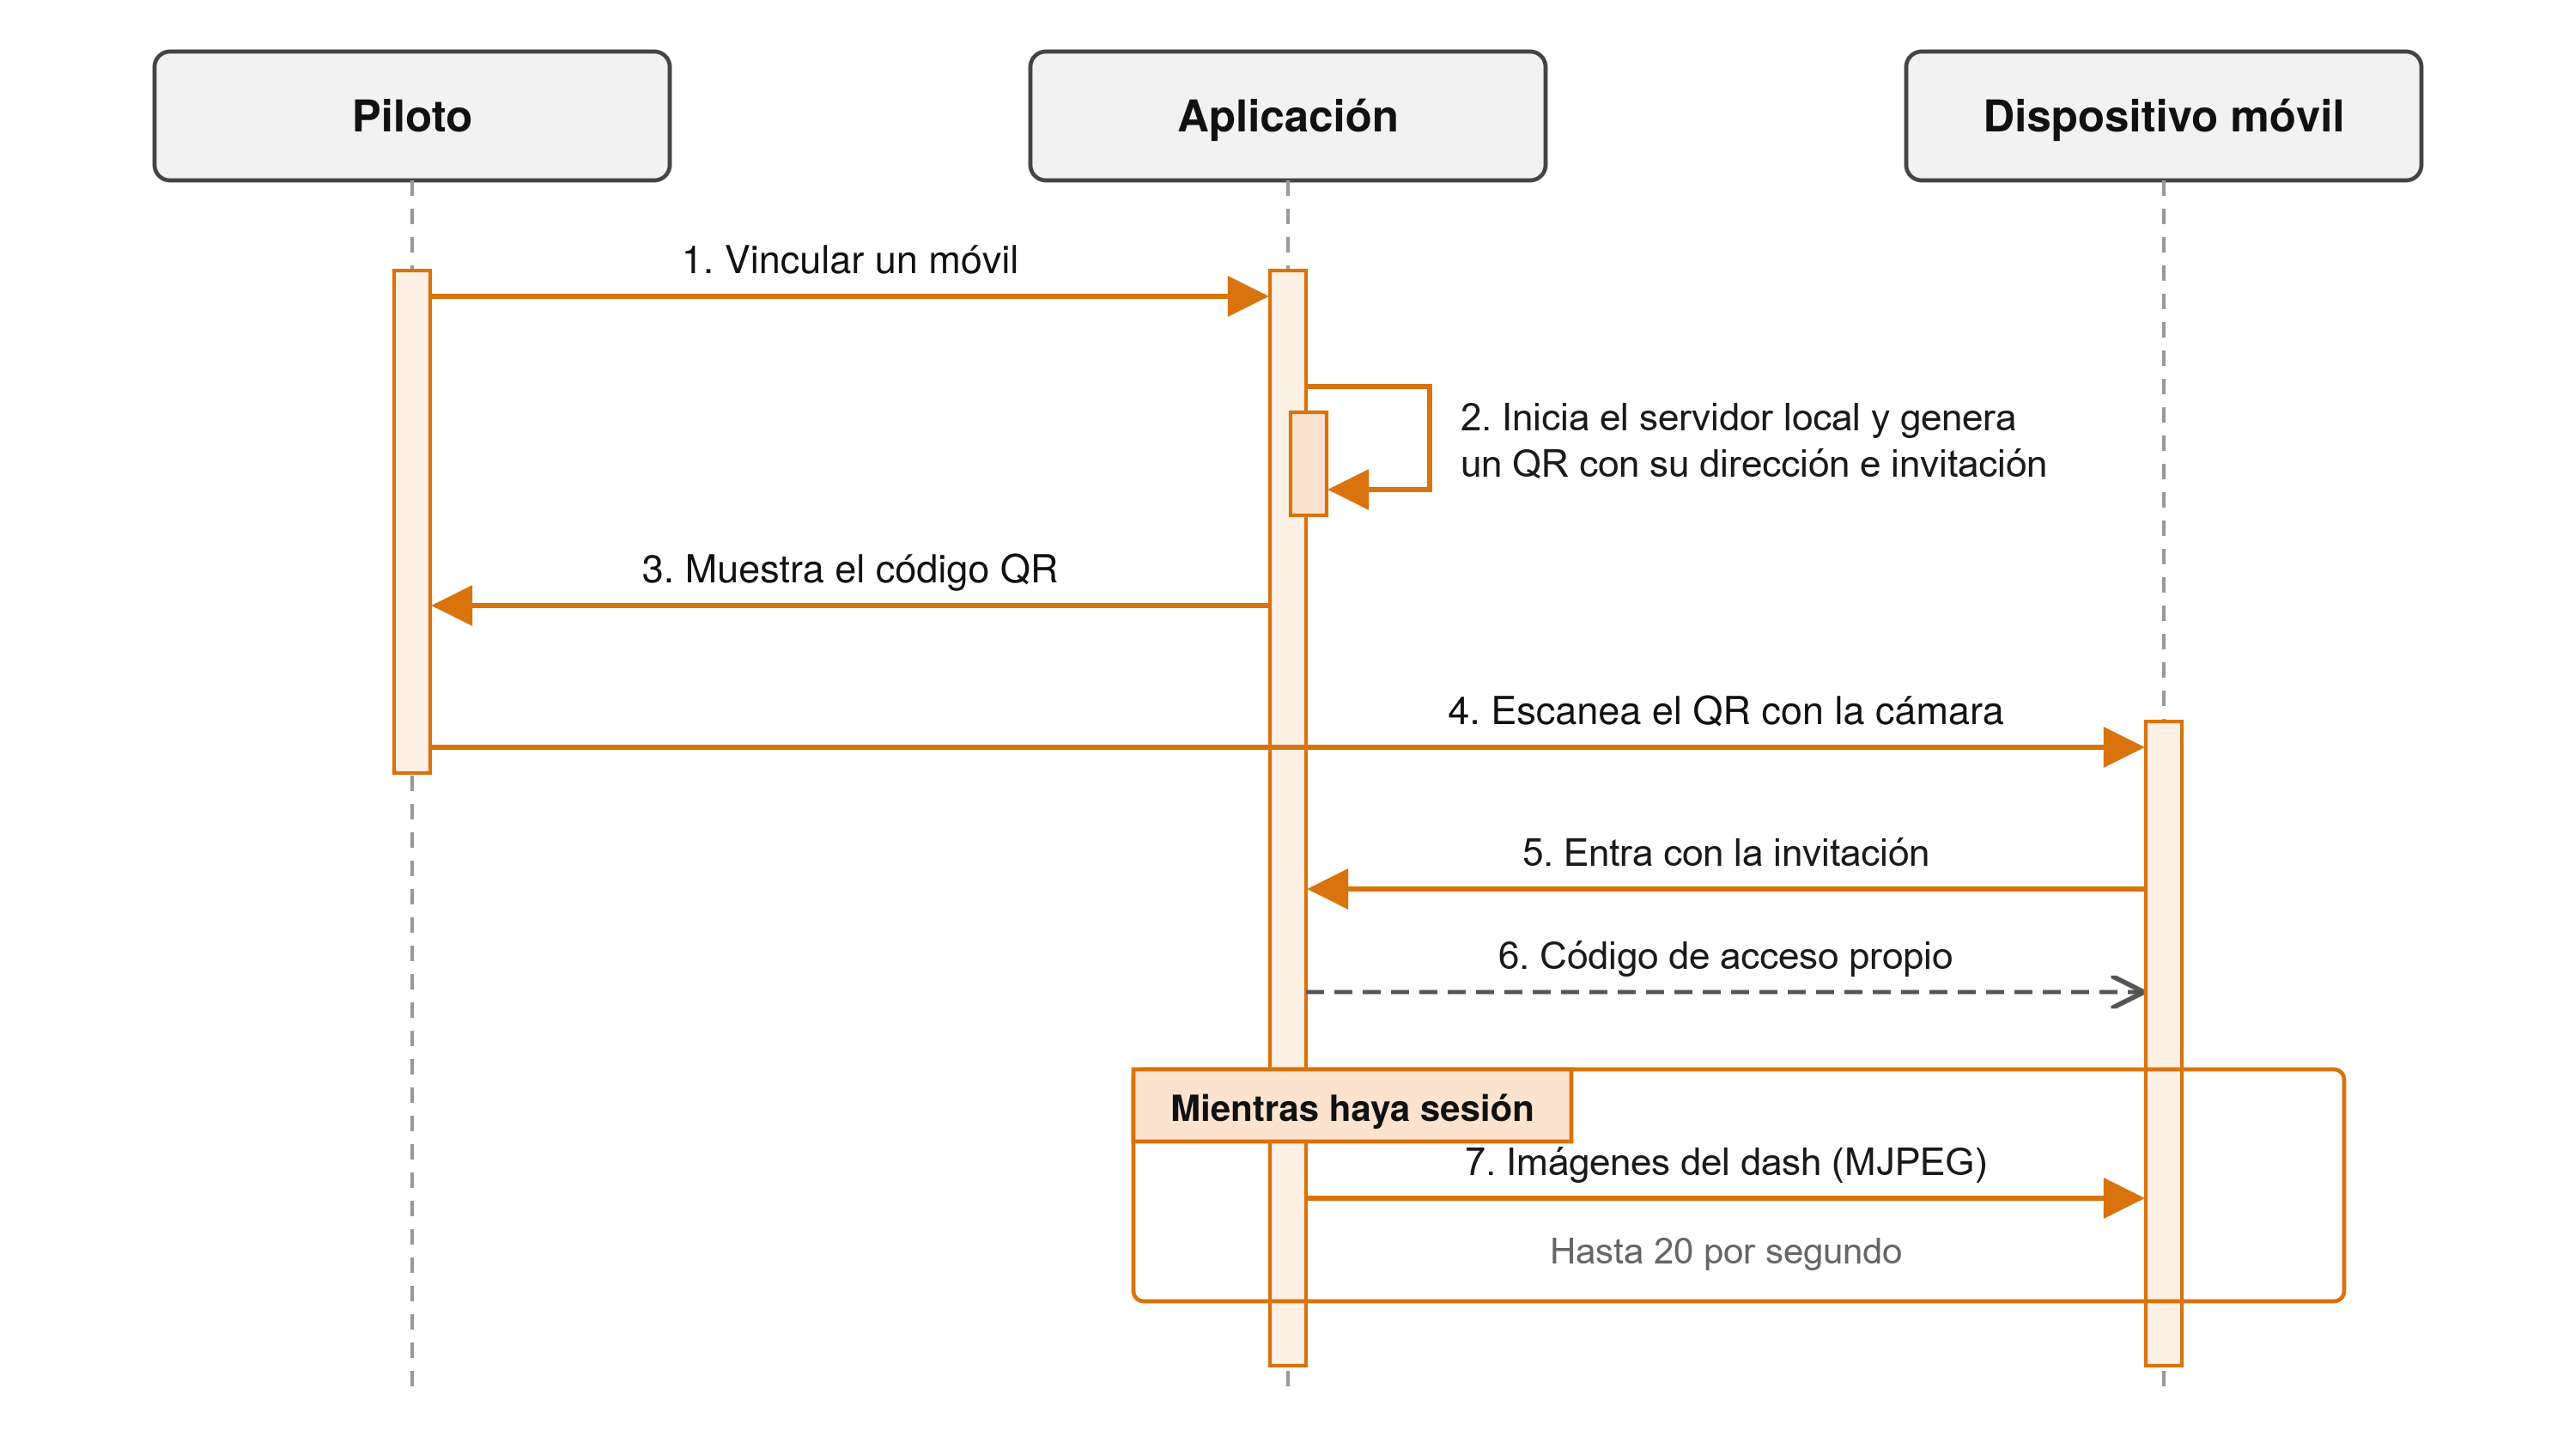
\includegraphics[width=0.9\textwidth]{img/secuencia-movil.png}
	\caption{Secuencia de vinculación y envío del \textit{dash} a un dispositivo móvil. (Fuente propia)}
	\label{fig:secuencia-movil}
\end{figure}

Dibujar el \textit{dash} en el ordenador y enviar las imágenes ya hechas evita tener que rehacer su motor de dibujo en el navegador: el móvil solo necesita una página mínima y muestra lo mismo que la pantalla del aro. A cambio, el tráfico es mayor que si se enviaran solo los valores, por lo que la aplicación ajusta las imágenes a un límite de ancho de banda y, si la red va lenta, descarta las que no llegan a tiempo en lugar de acumular retraso. Toda la comunicación se mantiene dentro de la red local, sin pasar por ningún servidor externo, de acuerdo con el requisito de privacidad RNF42.

\section{Diseño de la persistencia}
\label{sec:persistencia}
El sistema guarda sus datos en dos niveles. Cada \textbf{periférico} guarda en su propia memoria no volátil la configuración con la que funciona en ese momento, de modo que la conserva al desconectarlo y puede usarse sin la aplicación (RNF19 y RNF20). La \textbf{aplicación} guarda en el disco del ordenador todo lo demás: la biblioteca de perfiles entre los que el usuario puede elegir, sus propios ajustes, los \textit{dashes}, las estrategias y las sesiones grabadas.

La relación entre ambos niveles es sencilla: el periférico guarda una sola configuración, la activa, y la aplicación guarda todas las posibles. Cuando el usuario elige un perfil, o la aplicación lo aplica de forma automática al detectar el juego (RF31), la aplicación escribe sus valores en el periférico, que pasan a ser su nueva configuración activa. Esta sección describe qué se guarda en cada nivel, dónde y cuándo.

\subsection{Periféricos}
\label{subsec:persistencia-perifericos}
La base guarda sus datos en la memoria flash del STM32F405, y la pedalera y el aro, en la EEPROM de su ATmega32U4. La tabla~\ref{tab:persistencia-perifericos} recoge el contenido de cada una.

\begin{table}[H]
	\centering
	\caption{Datos guardados en la memoria de cada periférico.}
	\label{tab:persistencia-perifericos}
	\small
	\begin{tabularx}{\textwidth}{@{}>{\raggedright\arraybackslash}p{2.4cm}>{\raggedright\arraybackslash}p{1.8cm}X>{\raggedright\arraybackslash}p{3.2cm}@{}}
		\toprule
		\textbf{Periférico} & \textbf{Memoria} & \textbf{Datos} & \textbf{Cuándo se escribe} \\
		\midrule
		Base VH Grid DD15 & Flash & Ajustes del \textit{force feedback}: rango de giro, fuerza máxima, suavizado, tope, efectos base, ecualizador y curva. & Cinco segundos después del último cambio y al cerrar la aplicación. \\
		& & Configuración del motor y del encoder. & Junto con los ajustes. \\
		& & Tabla de compensación anti-cogging. & Al terminar la calibración. \\
		Pedalera VH Axis & EEPROM & Por cada pedal: reposo, fondo, zona muerta y los siete puntos de la curva de respuesta. & Al cambiar un ajuste o calibrar. \\
		Aro VH Formula Apex & EEPROM & Brillo de la tira. & Al cambiar el brillo. \\
		\bottomrule
	\end{tabularx}
\end{table}

La posición del centro del volante no se conserva entre sesiones, esto es debido a que el encoder es incremental, la base no conoce su posición absoluta al arrancar y toma como centro la posición en la que se enciende. En la pedalera, la inversión de un pedal no necesita un dato propio, porque se deduce de cuál de sus dos valores, reposo o fondo, es mayor.

En el aro no se guarda la asignación de luces por eventos ni los umbrales de revoluciones, porque solo tienen sentido con la telemetría y, por tanto, con la aplicación abierta. Tampoco el modo y el punto de mordida de las palancas de embrague. Todos ellos los guarda la aplicación (apartado~\ref{subsec:persistencia-aplicacion}).

El diseño de la persistencia en los periféricos responde a tres criterios:

\begin{itemize}
	\item \textbf{Proteger los ciclos de escritura.} Tanto la flash como la EEPROM admiten un número limitado de escrituras antes de degradarse, del orden de diez mil en la flash del STM32F405 y de cien mil en la EEPROM del ATmega32U4. Como un control deslizante de la aplicación puede enviar decenas de cambios en pocos segundos, cada cambio se aplica de inmediato en la copia de RAM, y la escritura en la memoria no volátil se limita de dos formas. En la EEPROM solo se escriben los bytes que realmente han cambiado (RNF22). En la flash, que se borra por sectores completos, la aplicación agrupa los cambios y pide guardar la configuración cinco segundos después del último. El bloque nuevo se añade a continuación del anterior, y un sector solo se borra cuando ya no queda sitio.
	\item \textbf{Separar los datos del programa.} En la base, la configuración y la tabla anti-cogging ocupan los dos últimos sectores de la flash, de 128~kB cada uno, reservados y distintos de los 768~kB del firmware. Así, al grabar una versión nueva solo se reescribe la zona del programa y se conserva la calibración, que de otro modo habría que repetir tras cada actualización (RNF24).
	\item \textbf{Arrancar siempre con datos válidos.} Los datos guardados llevan una marca que el firmware comprueba al arrancar, antes de usarlos. En la base es una suma de comprobación CRC-16 de toda la configuración, calculada junto con la versión de su formato, y en la pedalera y el aro, un valor fijo que identifica los datos. Si la comprobación falla, como en un periférico recién montado o, en la base, con datos dañados o de un formato incompatible, se cargan unos valores por defecto seguros en lugar de unos valores desconocidos, lo que en la base forma parte del arranque seguro (RNF14). Antes de recurrir a ellos, la base intenta leer los datos con el formato anterior, para que una actualización que cambie la estructura no pierda los ajustes ni la tabla anti-cogging.
\end{itemize}

\subsection{Aplicación}
\label{subsec:persistencia-aplicacion}
La aplicación guarda sus datos en ficheros junto al ejecutable, porque el programa se instala dentro de la carpeta de datos locales del usuario de Windows, en la ruta \texttt{\%LOCALAPPDATA\%\textbackslash\allowbreak{}VH~SimGrid\textbackslash\allowbreak{}ui\textbackslash\allowbreak{}configurador}. Esta ubicación tiene dos consecuencias. Por un lado, la aplicación se instala y escribe sus datos sin permisos de administrador (RNF25). Por otro, aunque programa y datos comparten carpeta, una actualización sustituye los ficheros del programa y el instalador no sobrescribe los perfiles y \textit{dashes} que ya existen ni toca los ajustes o las grabaciones, de modo que se conservan (RNF24). Todos los datos se quedan en el disco del usuario, sin enviarse a ningún servicio externo (RNF42). La tabla~\ref{tab:persistencia-aplicacion} resume lo que se guarda.

\begin{table}[H]
	\centering
	\caption{Datos guardados por la aplicación.}
	\label{tab:persistencia-aplicacion}
	\small
	\begin{tabularx}{\textwidth}{@{}>{\raggedright\arraybackslash}p{2.1cm}>{\raggedright\arraybackslash}p{4.4cm}X@{}}
		\toprule
		\textbf{Datos} & \textbf{Ubicación} & \textbf{Contenido} \\
		\midrule
		Ajustes de la aplicación & \texttt{ajustes.json} & Idioma, tema, arranque con Windows, segundo plano, reconexión automática, límite de grabaciones y configuración de voz y de avisos del ingeniero (RF36, RF45 y RF48). \\
		Perfiles & \texttt{perfiles/volante/}, \texttt{perfiles/pedales/}, \texttt{perfiles/aro/} & Un fichero por perfil y periférico. El del aro incluye la asignación de luces, el brillo y los ajustes de las palancas de embrague. En los ajustes se anota qué perfil de volante corresponde a cada juego y coche, y qué perfil de aro a cada juego (RF20 y RF31). \\
		\textit{Dashes} & \texttt{perfiles/dash/\allowbreak{}<nombre>/} & Diseño de cada \textit{dash} en \texttt{dash.json} (pantallas, elementos, propiedades y fórmulas), junto a sus imágenes y fuentes. Los 20 de serie se instalan en esta misma carpeta (RF40 y RF42). \\
		Estrategias & \texttt{perfiles/\allowbreak{}strategies/\allowbreak{}library.json} & Estrategias de carrera guardadas por juego, coche y circuito, con los datos de la carrera y las paradas (RF50 y RF52). \\
		Historial & \texttt{perfiles/sessions/}, \texttt{perfiles/references/}, \texttt{perfiles/mapas/} & Fichas por vuelta de cada sesión, vueltas de referencia y mapas de pista. \\
		Sesiones grabadas & \texttt{grabaciones/} & Telemetría cruda de cada sesión, con todos sus canales, y el índice de la lista de sesiones (RF53). \\
		\bottomrule
	\end{tabularx}
\end{table}

Se distinguen dos tipos de datos según su tamaño y su uso:

\begin{itemize}
	\item \textbf{Datos de configuración e historial}: todo salvo las grabaciones. Son pequeños y el usuario los modifica a menudo, por lo que se guardan en JSON, un formato de texto fácil de leer y de depurar. Se escriben primero en un fichero temporal, que después sustituye al definitivo de una sola vez, para que un corte de luz a mitad no deje un fichero dañado. Los \textit{dashes}, las estrategias y las fichas de sesión indican además la versión de su formato, y los perfiles combinados de versiones antiguas se convierten solos al arrancar.
	\item \textbf{Sesiones grabadas}: cada una contiene miles de muestras de cientos de canales, tomadas a 30~Hz, por lo que se guardan en texto JSON comprimido con gzip (\texttt{.jsonl.gz}). Cada línea es un instante y solo recoge los canales que han cambiado, lo que reduce mucho su tamaño. Para que el disco no se llene, la aplicación conserva un número máximo de grabaciones, 20 de fábrica y configurable por el usuario, además de un límite opcional de espacio, y borra las más antiguas al superarlo (RF53). La primera línea de cada grabación es una cabecera con el juego, el coche y el circuito, y el mejor tiempo se calcula una vez y se guarda en \texttt{indice.json}, lo que permite mostrar y filtrar la lista de sesiones sin abrir cada grabación (RF54).
\end{itemize}

Por último, la aplicación permite reunir sus datos en un solo fichero \texttt{.zip} de copia de seguridad, que el usuario puede guardar o llevar a otro ordenador y restaurar después (RF35). La copia incluye también las sesiones grabadas, porque son lo único que no se puede volver a generar, y deja fuera solo el certificado del dispositivo móvil, que lleva una clave privada y se crea de nuevo en cada equipo. Los \textit{dashes} pueden además exportarse e importarse de uno en uno en un fichero comprimido \texttt{.vhdash.zip}, para compartirlos con otros usuarios (RF43).

\section{Experiencia de usuario (UX)}
\label{sec:ux}
El usuario objetivo de VH SimGrid es un piloto aficionado, no un tecnico (tabla~\ref{tab:actores}). Debe poder utilizar, calibrar y poner en marcha el equipo sin necesidad de tener conocimientos de programación o electronica (RNF26). Por eso la experiencia de usuario no se limita al aspecto de las pantallas, que se trata en la sección~\ref{sec:ui}, sino que abarca cómo se desarrollan los pasos que tiene cada una, en qué orden, qué ve el piloto en cada momento y qué ocurre cuando algo sale mal.

El diseño de la interacción se apoya en las heurísticas de usabilidad de Nielsen~\cite{nielsen1994}, adaptadas al contexto del simracing. La tabla~\ref{tab:principios-ux} recoge los principios aplicados y cómo se reflejan en el sistema.

\begin{table}[H]
	\centering
	\caption{Principios de experiencia de usuario aplicados en VH SimGrid.}
	\label{tab:principios-ux}
	\small
	\begin{tabularx}{\textwidth}{@{}>{\raggedright\arraybackslash}p{3.6cm}X@{}}
		\toprule
		\textbf{Principio} & \textbf{Aplicación en el sistema} \\
		\midrule
		Funcionar al conectar & Los periféricos se detectan y se configuran solos, y la aplicación lee su estado real en lugar de pedírselo al usuario (RF29). \\
		Visibilidad del estado & Cada acción tiene una respuesta visible: la traza en vivo de los pedales, la vista previa de los LEDs, el estado de cada periférico o el perfil activo (RNF28). \\
		Guiar en lugar de configurar & Las tareas con varios pasos, como la puesta en marcha o la calibración, se resuelven con asistentes que piden una sola acción cada vez. \\
		Lenguaje del piloto & Los valores se expresan en las unidades que entiende el piloto, como los kilos en el freno o los grados de giro, y no en lecturas del sensor. \\
		Prevención de errores & Los valores fuera de rango se limitan, el firmware se comprueba antes de grabarlo y las lecturas dudosas se repiten (RNF15 y RNF39). \\
		Control del usuario & Toda tarea guiada puede posponerse o cerrarse y reanudarse después, y toda decisión automática puede cambiarse a mano. \\
		Sin soltar el volante & Lo que se necesita durante la conducción se maneja con los mandos del aro o por voz (RNF29). \\
		\bottomrule
	\end{tabularx}
\end{table}

Los apartados siguientes describen los cuatro flujos en los que estos principios tienen más peso. Cada uno se representa con un diagrama de flujo y se corresponde con un caso de uso del capítulo~\ref{cap:requisitos}.

\subsection{Primera configuración}
\label{subsec:ux-asistente}
La primera vez que se abre la aplicación, un asistente guía al piloto por la puesta en marcha completa del equipo (RF33), siguiendo el caso de uso CU1. Su flujo se muestra en la figura~\ref{fig:ux-asistente}.

\begin{figure}[H]
	\centering
	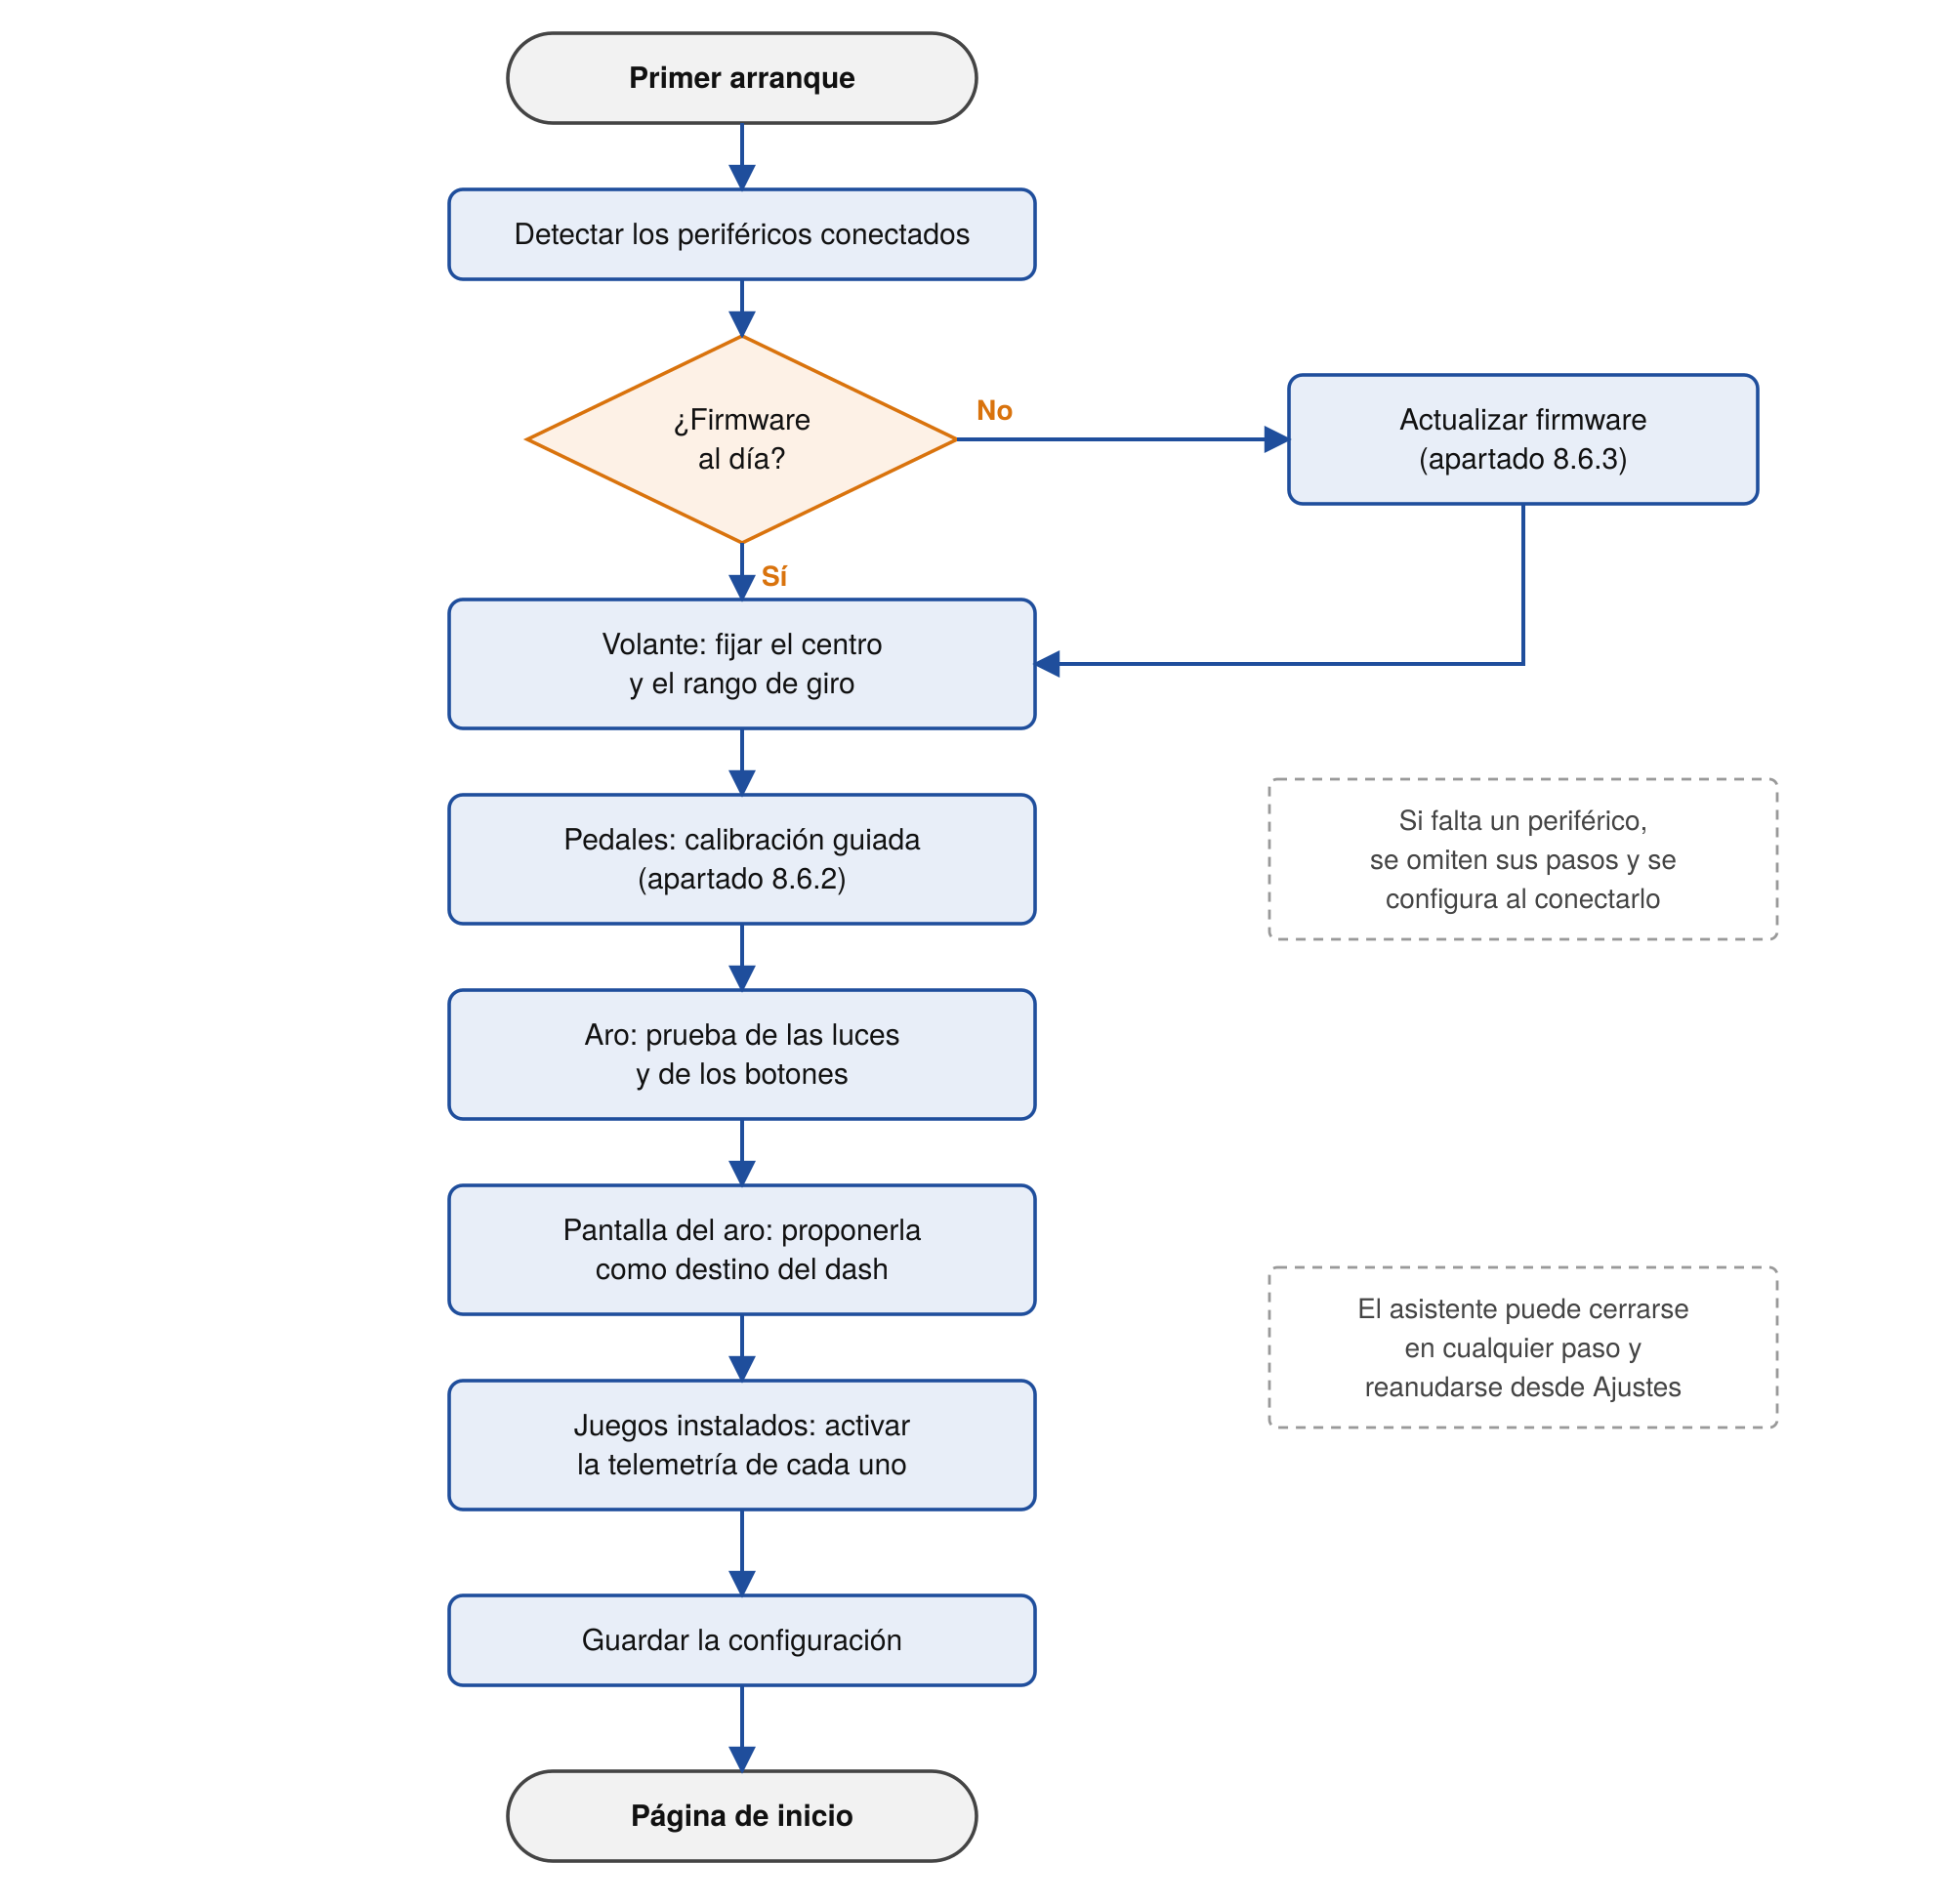
\includegraphics[width=0.8\textwidth]{img/ux-asistente.png}
	\caption{Flujo del asistente de primera configuración. (Fuente propia)}
	\label{fig:ux-asistente}
\end{figure}
El diseño del asistente responde a varias decisiones:

\begin{itemize}
	\item \textbf{Un paso por periférico, en orden de importancia.} El asistente empieza por el volante, sigue con los pedales y el aro, y termina con la pantalla del aro y los juegos. Cada paso pide una sola acción y muestra el resultado antes de pasar al siguiente, de modo que el piloto nunca tiene que recordar qué hizo antes.
	\item \textbf{El firmware primero.} Antes de configurar nada, el asistente comprueba que cada periférico tiene la última versión de firmware y, si no la tiene, ofrece actualizarlo. Así se evita calibrar un periférico con un firmware que va a cambiar justo después.
	\item \textbf{Adaptado a lo que hay conectado.} Si falta un periférico, el asistente omite sus pasos en lugar de detenerse, y lo configura cuando se conecte. Quien solo tiene la pedalera puede completar el asistente igual que quien tiene el equipo completo.
	\item \textbf{Las tareas fuera de la aplicación, explicadas.} Activar la telemetría depende de cada juego y no puede hacerlo la aplicación. Para ese paso, el asistente detecta los juegos instalados y explica, para cada uno, qué opción hay que activar.
	\item \textbf{Siempre se puede salir.} El asistente puede cerrarse en cualquier paso y reanudarse más tarde desde los ajustes de la aplicación.
\end{itemize}

\subsection{Calibración de los pedales}
\label{subsec:ux-calibracion}
La calibración indica a la pedalera dónde empieza y dónde acaba el recorrido de cada pedal y qué fuerza máxima se quiere aplicar en el freno (RF12). Sigue el caso de uso CU3 y su flujo se representa en la figura~\ref{fig:ux-calibracion}.

\begin{figure}[H]
	\centering
	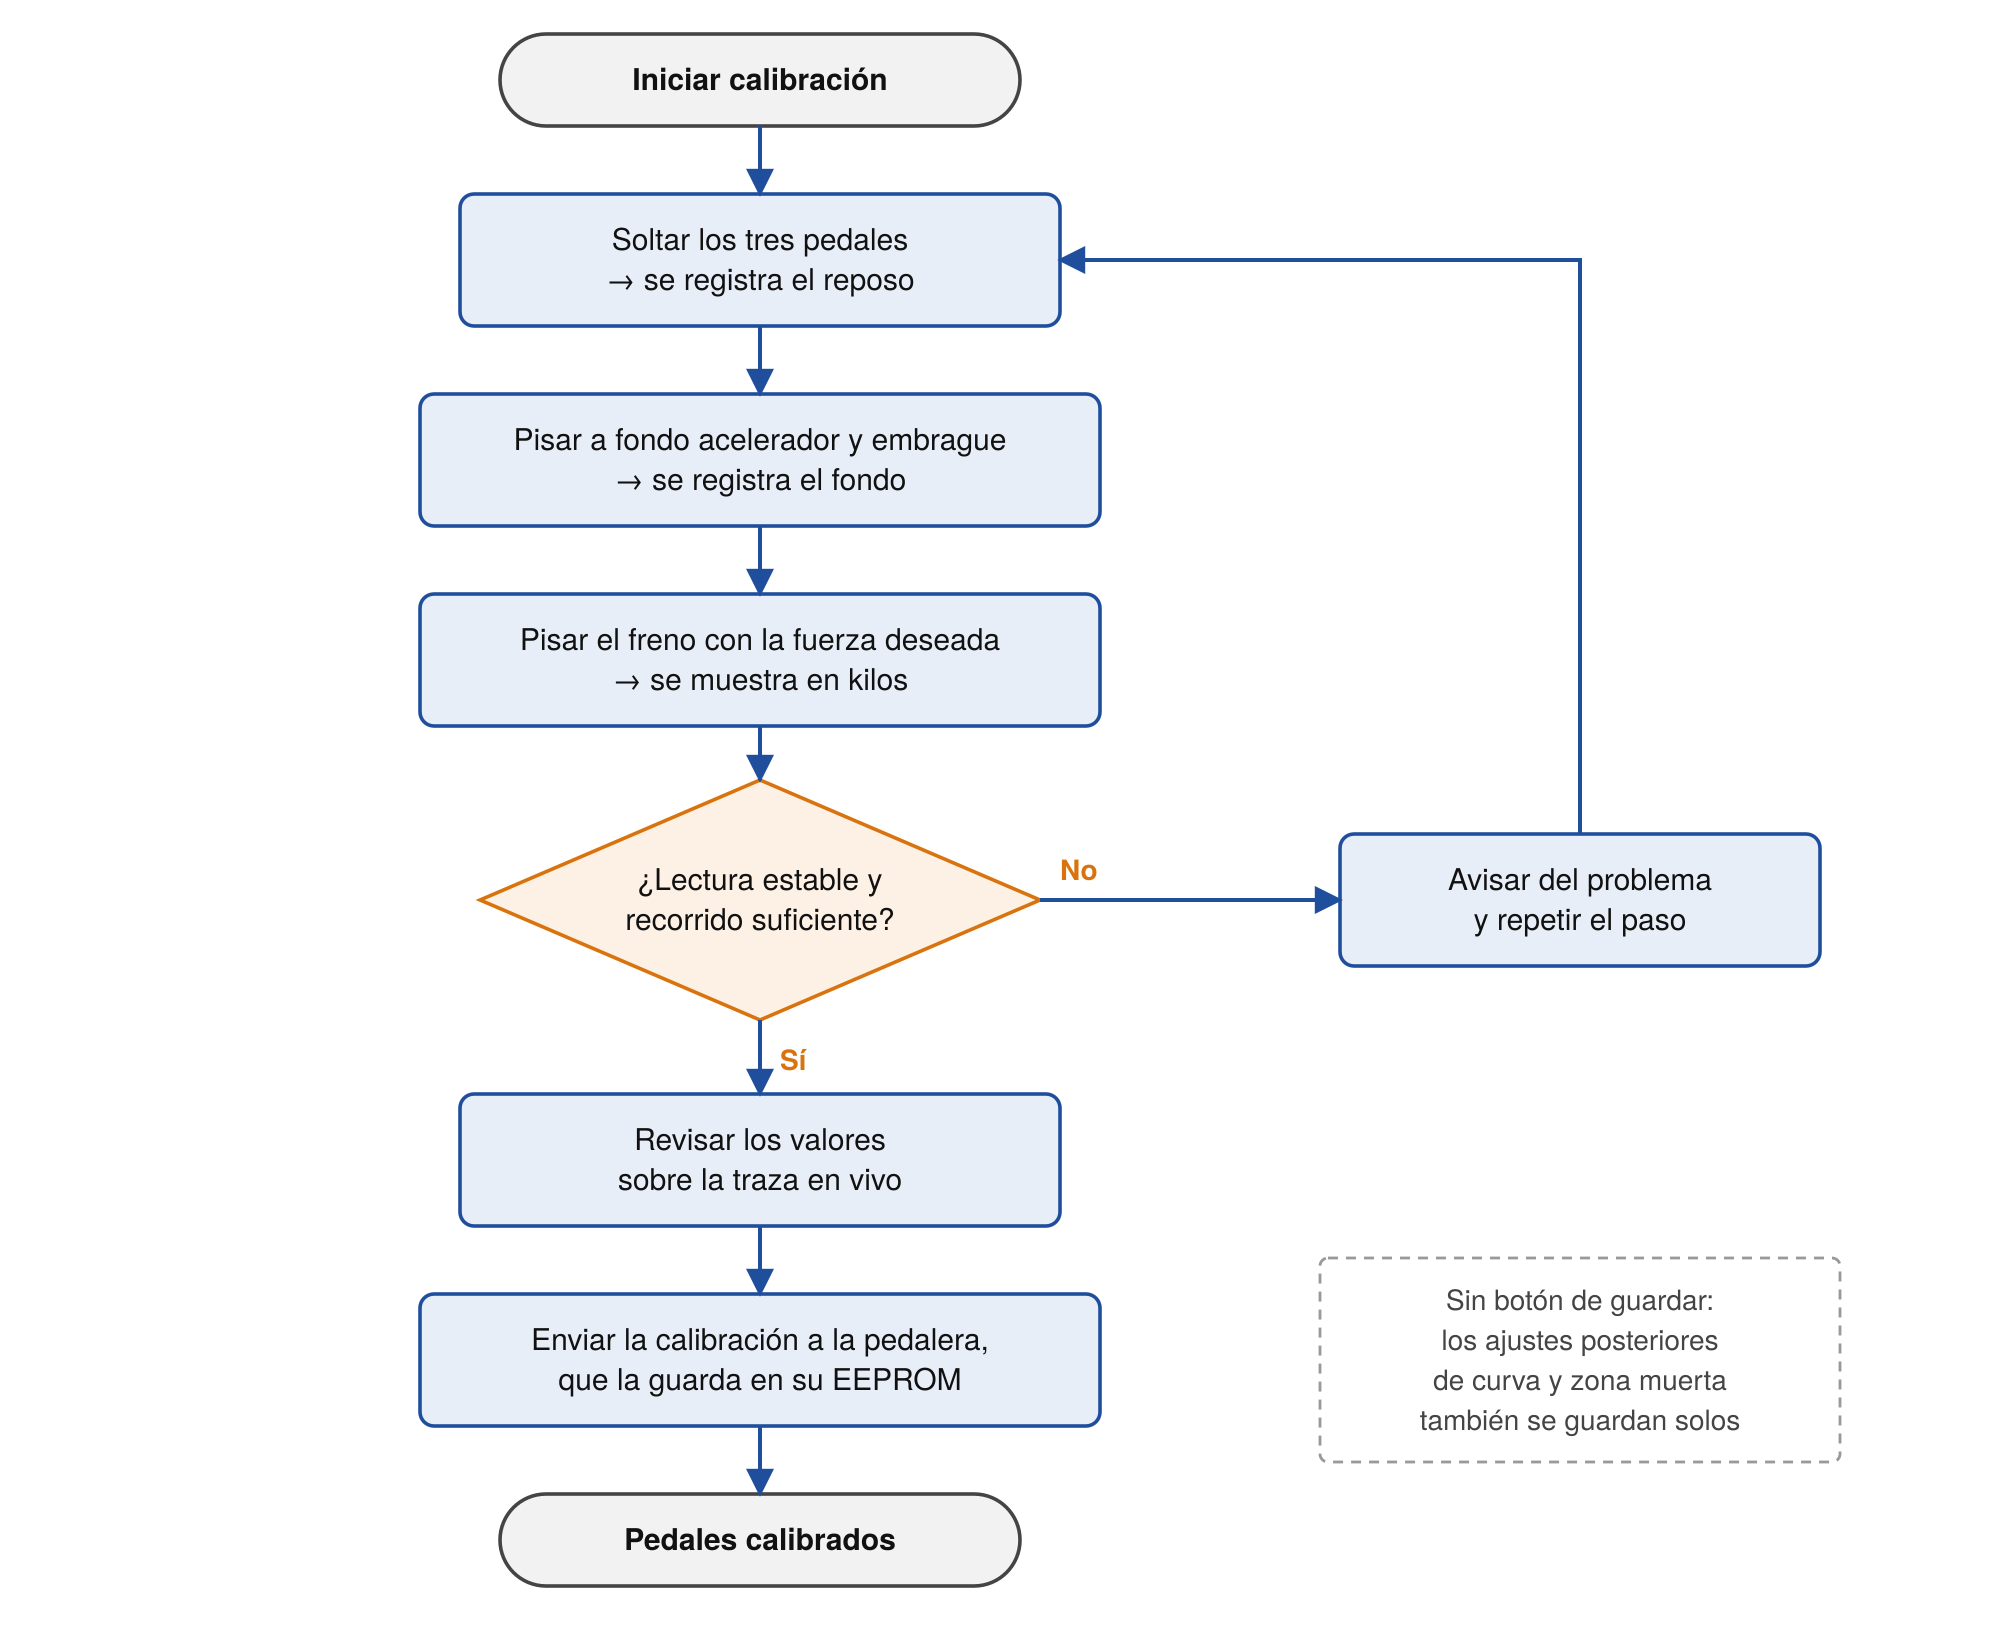
\includegraphics[width=0.8\textwidth]{img/ux-calibracion.png}
	\caption{Flujo de la calibración guiada de los pedales. (Fuente propia)}
	\label{fig:ux-calibracion}
\end{figure}

En una calibración tradicional, el usuario introduce a mano los valores mínimo y máximo de cada eje, unos números que no significan nada para un piloto. La calibración de VH SimGrid sustituye esos números por acciones físicas: soltar los pedales, pisarlos a fondo y frenar con la fuerza deseada. La aplicación toma cada lectura de la traza en vivo, de modo que el piloto ve en todo momento cómo responde el pedal mientras lo pisa, y después envía los valores a la pedalera con el mensaje de calibración (apartado~\ref{subsec:protocolo-pedalera-aro}).

El freno merece un tratamiento propio. Como mide la fuerza y no el recorrido, su fondo no es una posición física, sino la fuerza máxima con la que el piloto quiere frenar, que la aplicación muestra en kilos. Así el piloto decide la dureza del freno en una unidad que entiende, y puede reconocer de un vistazo si ha calibrado un freno blando o uno firme.

La aplicación comprueba además cada lectura antes de aceptarla. Si la señal es inestable, porque el pie aún se mueve, o el recorrido es demasiado corto para ser un pedal pisado a fondo, avisa del problema y repite el paso, en lugar de guardar una calibración que haría que el pedal no llegara nunca al 100~\%. Por último, la calibración y los ajustes que se hagan después, como la curva o la zona muerta, se guardan solos en la pedalera, sin un botón de guardar que el piloto pueda olvidar pulsar (RF14).

\subsection{Actualización de firmware}
\label{subsec:ux-firmware}
Actualizar el firmware de un microcontrolador suele exigir herramientas específicas, poner la placa en modo de grabación a mano y saber qué fichero corresponde a cada dispositivo. VH SimGrid reduce todo eso a una sola decisión del piloto: aceptar o no la actualización (RF32). El flujo, que sigue el caso de uso CU5, se muestra en la figura~\ref{fig:ux-firmware}.

\begin{figure}[H]
	\centering
	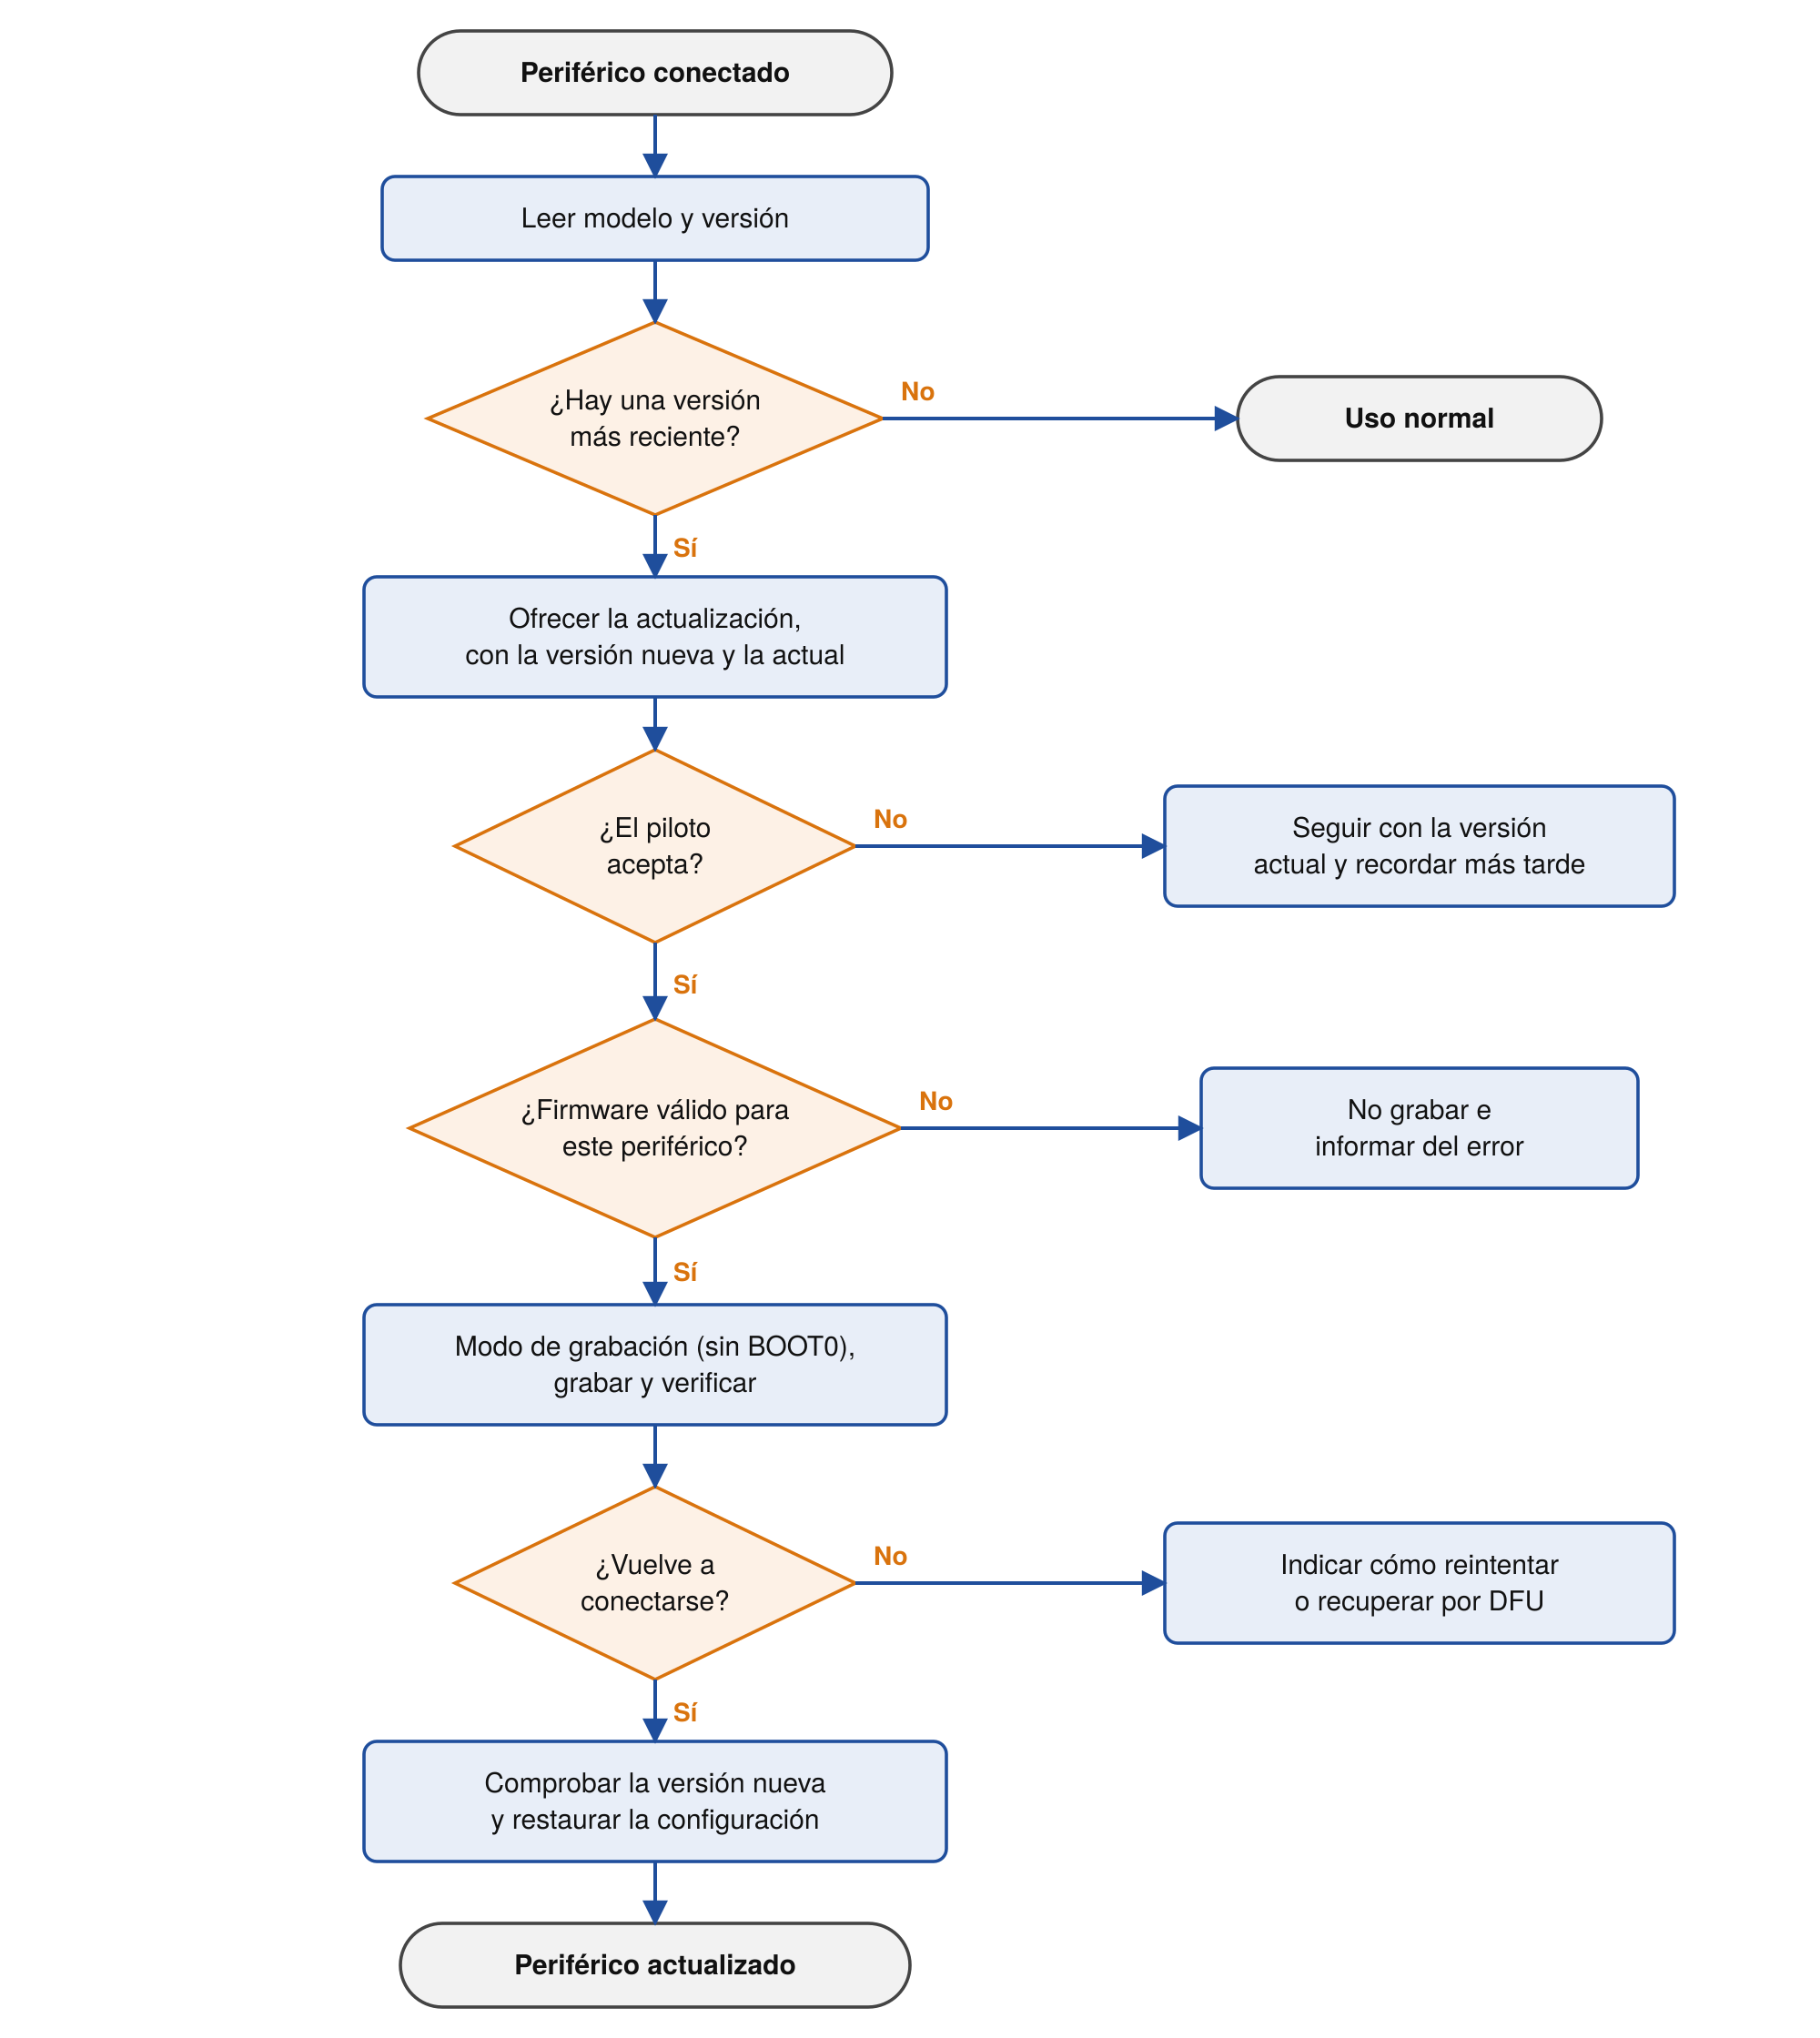
\includegraphics[width=0.75\textwidth]{img/ux-firmware.png}
	\caption{Flujo de la actualización de firmware de un periférico. (Fuente propia)}
	\label{fig:ux-firmware}
\end{figure}

Las decisiones de diseño más relevantes son las siguientes:

\begin{itemize}
	\item \textbf{Ofrecer, no imponer.} La aplicación compara la versión del periférico con la que incluye al conectarlo, y si hay una más reciente lo comunica y deja la decisión al piloto, mostrando ambas versiones. Si la pospone, el periférico sigue funcionando con su versión actual, y la aplicación lo recuerda más adelante. De este modo, una actualización nunca interrumpe una sesión.
	\item \textbf{Sin intervención física.} La aplicación pone ella misma el periférico en modo de grabación mediante una orden de su canal de configuración. En la base, esto evita abrir la carcasa para colocar el puente BOOT0, y en la pedalera y el aro, instalar herramientas externas.
	\item \textbf{Comprobar antes de grabar.} La aplicación elige el firmware según la identidad USB del periférico y comprueba que el fichero le corresponde y no está dañado. Si no supera la comprobación, no se graba, porque un firmware equivocado podría dejar el periférico inutilizable (RNF15).
	\item \textbf{Conservar la configuración.} Tras la grabación, la aplicación vuelve a conectar el periférico, comprueba la nueva versión y le restaura la configuración del usuario, de modo que el piloto no tiene que volver a calibrar nada (RNF24).
	\item \textbf{Un camino de recuperación.} Si el periférico no vuelve a conectarse, la aplicación indica cómo reintentar la grabación y, como último recurso, cómo recuperarlo por DFU, la única operación que requiere la intervención del constructor (CU6).
\end{itemize}

\subsection{Perfiles automáticos}
\label{subsec:ux-perfiles}
Cada juego, e incluso cada coche, se conduce mejor con unos ajustes distintos: un GT3 pide un \textit{force feedback} y un rango de giro diferentes a los de un monoplaza o un coche de rally. Los perfiles automáticos evitan que el piloto tenga que cambiar estos ajustes a mano cada vez que cambia de juego o de coche (RF31). Su funcionamiento se representa en la figura~\ref{fig:ux-perfiles}.

\begin{figure}[H]
	\centering
	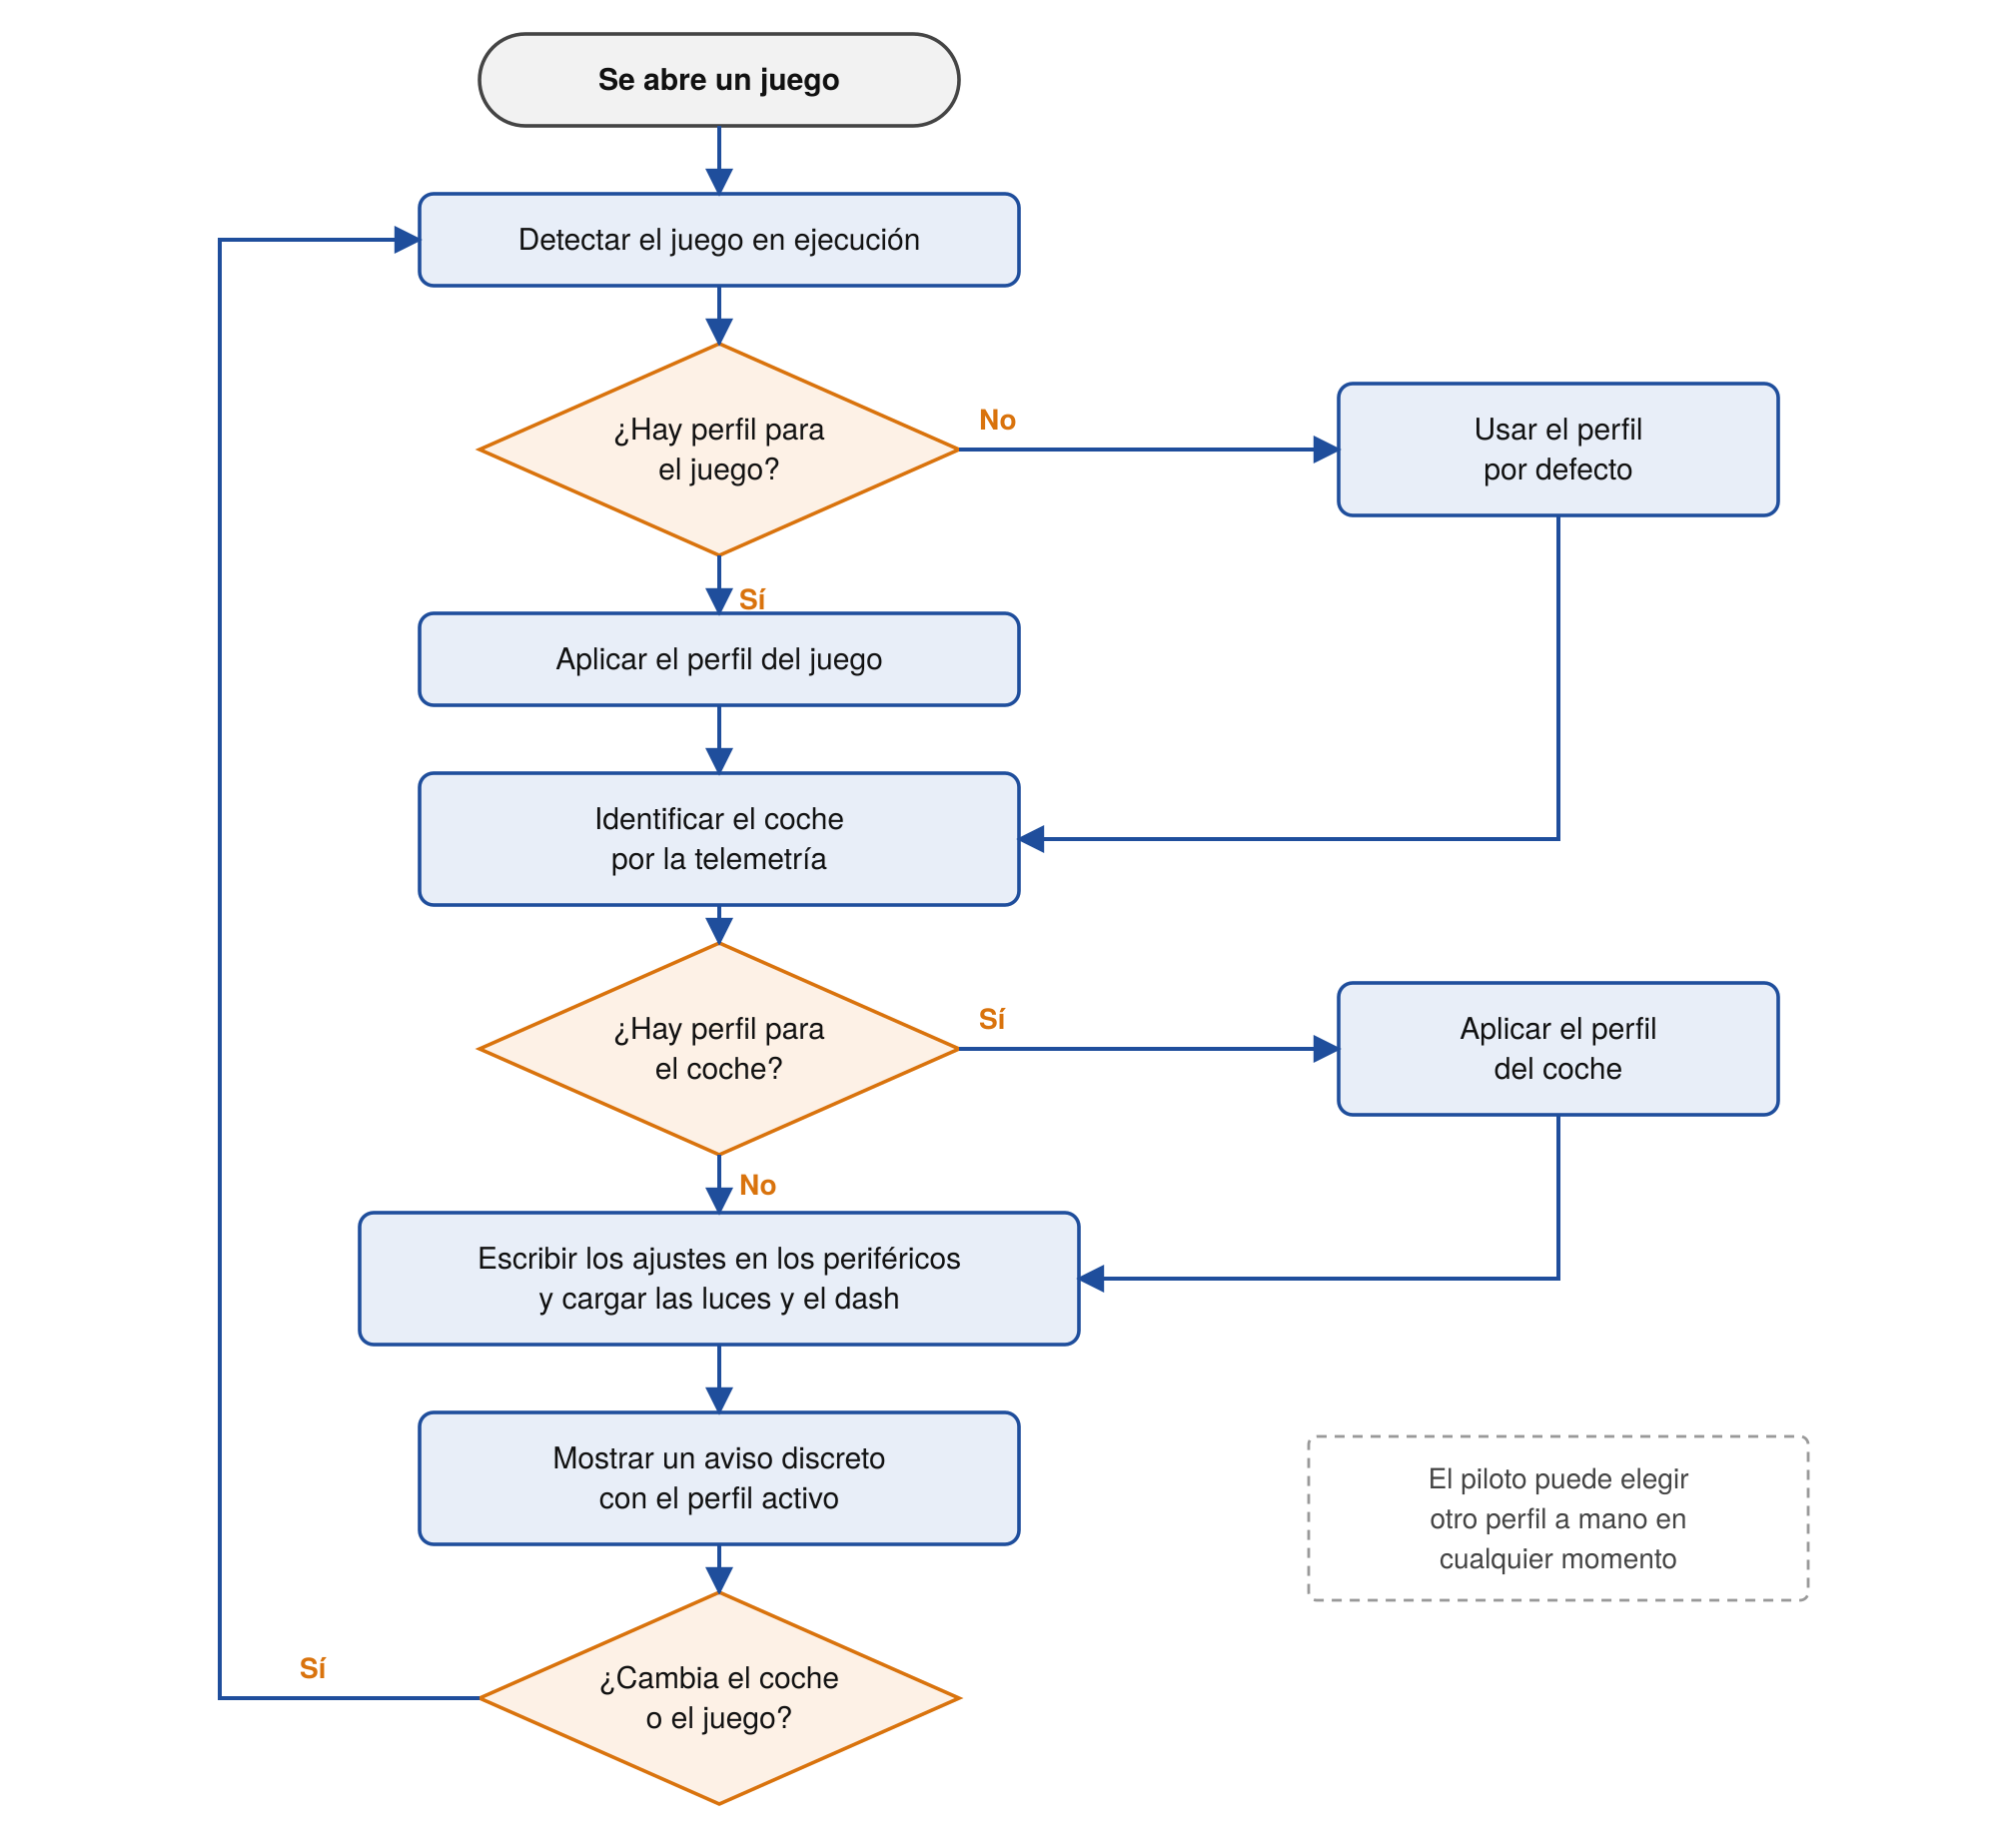
\includegraphics[width=0.8\textwidth]{img/ux-perfiles.png}
	\caption{Flujo de la aplicación automática de perfiles. (Fuente propia)}
	\label{fig:ux-perfiles}
\end{figure}

La selección del perfil se hace en dos niveles, del más general al más concreto. Cuando la aplicación detecta que se ha abierto un juego, aplica el perfil asociado a ese juego o, si no tiene ninguno, el perfil por defecto. Después, cuando la telemetría identifica el coche, comprueba si existe un perfil específico para él y, si existe, lo aplica en lugar del anterior. Este orden permite que el piloto configure solo lo que necesita: un perfil por juego cubre la mayoría de los casos, y los perfiles por coche quedan para las excepciones.

Aplicar un perfil no se limita a los ajustes de los periféricos. Con ellos se cargan también la asignación de luces del aro y el \textit{dash} asociado, que se abre en la pantalla del aro (RF20 y RF27), de modo que todo el equipo cambia a la vez. El proceso se repite cada vez que cambia el coche o el juego.

Como toda decisión automática, el cambio de perfil debe ser visible y reversible. La aplicación muestra un aviso discreto con el nombre del perfil aplicado, que informa al piloto sin interrumpirle, y el piloto puede elegir otro perfil a mano en cualquier momento, desde la aplicación o desde la pantalla del aro (RF25).


\section{Interfaces de usuario (UI)}
\subsection{Estructura general}
\subsection{Página de inicio}
\subsection{Página de configuración de la base}
\subsection{Página de configuración del aro}
\subsection{Página de configuración de la pedalera}
\subsection{Biblioteca de dash y editor}
\subsection{Ingeniero de pista}
\subsection{Análisis de la telemetría}
\subsection{Ajustes de la aplicación}

\section{Guía de estilos}
\subsection{Paleta de colores}
\subsection{Tipografía}
\subsection{Iconografía}
\subsection{Componentes reutilizables}

\section{Diseño de pruebas y validación}
	% !TeX root = ../main.tex
\chapter{Implementación}
Texto.

\section{Entorno y estructura del proyecto}
Texto.

\section{Implementación de los componentes}
\subsubsection{Componente 1}
Texto.

\section{Desafíos encontrados y soluciones adoptadas}
Texto.

	% !TeX root = ../main.tex
\chapter{Resultados y análisis}
Texto.

\section{Resultados de las pruebas y validación}
Texto.

\section{Análisis de los resultados}
Texto.

	% !TeX root = ../main.tex
\chapter{Conclusiones}
\label{cap:conclusiones}
Texto \citapendiente{}.

\section{Trabajo futuro}
Texto.


	% ---------- APÉNDICES ----------
	\appendix
	% !TeX root = ../main.tex
\chapter{Título del apéndice}
\label{ap:a}

Contenido del apéndice.


	% ---------- BIBLIOGRAFÍA ----------
	\setlength{\bibitemsep}{1em}
	\printbibliography[heading=bibintoc, title={Bibliografía}]

	% ---------- GLOSARIO ----------
	\printglossary[title=Glosario]

\end{document}
